\documentclass[12pt,a4paper]{article}
\usepackage[utf8]{inputenc}
\usepackage[italian]{babel}
\usepackage{amsmath}
\usepackage{amsfonts}
\usepackage{amssymb}
\usepackage{amsthm}
\usepackage[pagebackref=true]{hyperref}
\usepackage{graphicx}
\usepackage{epstopdf}
\usepackage{latexsym}
\usepackage{fullpage}
\usepackage{quoting}
\usepackage{booktabs}
\usepackage{slashed}
\usepackage{feynmp-auto}
\theoremstyle{definition}
\newtheorem{thm}{Teorema}
\newtheorem{dfn}{Definizione}[section]
\newtheorem{exm}{Esempio}
\newtheorem{lem}{Lemma}
\newcommand{\pdev}[3][]{\frac{\partial^{#1} #2}{\partial #3^{#1}}}
\newcommand{\dev}[3][]{\frac{\mathrm{d}^{#1} #2}{\mathrm{d} #3^{#1}}}
\newcommand{\ham}{\mathcal{H}}
\newcommand{\lag}{\mathcal{L}}
\newcommand{\Div}{\mathrm{div}}
\newcommand{\grad}{\mathrm{grad}}
\newcommand{\diff}[1][]{\mathrm{d}#1}
\newcommand{\bra}{\langle}
\newcommand{\ket}{\rangle}
\newcommand{\bnabla}{\boldsymbol{\nabla}}
\newcommand{\Sch}{Schrödinger}
\newcommand{\adj}[1]{#1^{\dagger}}
\newcommand{\tr}{\mathrm{tr}}
\newcommand{\conn}[3]{\Gamma^{#1}_{#2 #3}}
\newcommand{\zpart}{\mathcal{Z}}
\quotingsetup{font=small}
\numberwithin{equation}{section}

\begin{document}
\begin{titlepage}
\centering
{\Huge \scshape{Cromodinamica Quantistica}}\\
\vspace*{0.5cm}
{\small Appunti (non rivisti) delle lezioni del professor Meggiolaro}
\vspace*{\stretch{0.5}} \\

\includegraphics[width=250pt,keepaspectratio=true]{Addons/eigenLibrichiaro}
\begin{center}
un progetto di
\end{center}

\includegraphics[width=250pt,keepaspectratio=true]{Addons/eigenlabinvertito2.png} \\
\url{www.eigenlab.org}
\vspace*{\stretch{1}} \\
{\small a cura di}\\
\vspace*{0.5cm}
{\normalsize Francesco Cicciarella\par}
\end{titlepage}
\pagebreak
\pagenumbering{roman}

\section*{Note legali}
\begin{center}
\begin{figure}[htbp]
\centering

\includegraphics[scale=1]{Addons/88x31.png}
\end{figure}
\vspace{0.5cm}
Copyright \copyright \; 2013-2014 di Francesco Cicciarella \\
\textit{Appunti di Cromodinamica Quantistica} \\	
è rilasciato sotto i termini della licenza \\
Creative Commons Attribuzione - Non commerciale - Condividi allo stesso modo 3.0 Italia. \\
Per visionare una copia completa della licenza, visita \\
\url{http://creativecommons.org/licenses/by-nc-sa/3.0/it/legalcode}
\end{center}
\section*{Liberatoria, mantenimento e segnalazione errori}
Questo documento viene pubblicato, in formato elettronico, senza alcuna garanzia di correttezza del suo contenuto. Il testo, nella sua interezza, è opera di \\

\vspace{0.3cm}
\begin{flushleft}
\texttt{Francesco Cicciarella}\\
\texttt{<f[DOT]cicciarella[AT]inventati[DOT]org>}
\end{flushleft}
\vspace{0.3cm}
e viene mantenuto dallo stesso, a cui possono essere inviate eventuali segnalazioni di errori.
\vspace{1cm}
\begin{flushright}
Pisa, 12 Febbraio 2014
\end{flushright}
\pagebreak


\tableofcontents
\pagebreak
\pagenumbering{arabic}
\section{$SU(N)$}
\begin{dfn}
$SU(N)$ è definito come il gruppo delle matrici $U$ $N\times N$ unitarie, cioè tali che $\adj{U}U=U\adj{U}=\mathbb{I}$ (da cui segue che $\adj{U}=U^{-1}$), aventi $\det U=+1$.
\end{dfn}

È sempre possibile scrivere un elemento $U\in SU(N)$ come $U=e^A$, con $A$ matrice $N\times N$. La condizione $\adj{U}=U^{-1}$ impone una condizione su $A$:
$$
\adj{U}=e^{\adj{A}}=e^{-A}=U^{-1}\qquad \Longrightarrow \qquad \adj{A}=-A\;,
$$
ossia $A$ è una matrice \emph{antihermitiana}. Inoltre la condizione sul determinante di $U$ impone che:
$$
\det U=e^{\tr A}=1\qquad \Longrightarrow\qquad \tr\, A=0\;.
$$
Riassumendo, $A$ deve essere una matrice antihermitiana a traccia nulla. È molto più conveniente (in virtù del significato fisico) scrivere $A=iH$, con $H$ matrice hermitiana; in definitiva, un generico elemento $U\in SU(N)$ può essere scritto come $U=e^{iH}$ con $H$ matrice $N\times N$ hermitiana a traccia nulla. Le matrici hermitiane $N\times N$ a traccia nulla sono identificate da $N^2-1$ parametri reali, ossia è uno spazio di dimensione $N^2-1$:
\begin{equation}
H=\sum_{a=1}^{N^2-1}\epsilon_a F_a\;,
\end{equation}
dove $\epsilon_a\in\mathbb{R}$ e $\{F_a, a=1,\ldots,N\}$ sono i \emph{generatori del gruppo}. L'elemento $U$ del gruppo a questo punto è identificato dagli $\epsilon_a$:
\begin{equation}
U=\exp\left(i\sum_{a=1}^{N^2-1}\epsilon_aF_a\right)\;.
\end{equation}
$SU(N)$ è un gruppo di Lie; in quanto gruppo, è chiuso rispetto al prodotto di elementi, cioè se $U_1,U_2\in SU(N)$, allora $U_3\equiv U_1U_2\in SU(N)$. La chiusura rispetto al prodotto degli elementi implica che i generatori del gruppo soddisfino l'\emph{algebra di Lie}:
\begin{equation}
[F_a,F_b]=iC^c_{ab}F_c\;.
\end{equation}
$C_{ab}^c$ sono costanti reali, dette \emph{costanti di struttura del gruppo}. Dalle proprietà di antisimmetria del commutatore, segue che $C_{ab}^c=-C^c_{ba}$ (sulle altre coppie di indici non possiamo dire nulla per adesso). I generatori $F_a$ e i parametri associati $\epsilon_a$, ossia la rappresentazione, non sono univocamente determinati. Si può scegliere quindi una rappresentazione più congeniale a seconda della situazione. L'esistenza di una rappresentazione "comoda" ci è garantita dal seguente:
\begin{thm} Se esiste una rappresentazione hermitiana dei generatori $F_a$, allora esiste una rappresentazione dei generatori $\hat{F}_a=\lag_{ab}F_b$, dove $\lag$ è una matrice reale, tale che:
\begin{itemize}
\item $\hat{F}_a$ sia hermitiana e a traccia nulla per ogni $a$;
\item $\hat{C}^c_{ab}$ siano antisimmetrici in tutti e tre gli indici;
\item la forma quadratica $g_{ab}\equiv\tr[\hat{F}_a\hat{F}_b]$ risulti essere definita positiva. In altre parole esiste un $\lambda>0$ dipendente dalla normalizzazione tale che:
\begin{equation}
g_{ab}=\tr[\hat{F}_a\hat{F}_b]=\lambda\delta_{ab}\;.
\end{equation}
\end{itemize}
\end{thm}
Alla luce di questo teorema possiamo dare la seguente:
\begin{dfn}[Rappresentazione definente di $SU(N)$]
\begin{align}
&[F_a,F_b]=if_{abc}F_c &f_{abc}\;\mbox{completamente antisimmetrico}\;, \notag \\
&\tr[F_aF_b]=\frac{1}{2}\delta_{ab} &\mbox{normalizzazione}\;.
\end{align}
\end{dfn}
Diamo altre tre definizioni importanti:
\begin{dfn}[Sottoalgebra di Cartan]
La sottoalgebra di Cartan di un gruppo di Lie è la sottoalgebra generata dai generatori del gruppo che commutano fra di loro.
\end{dfn}
\begin{dfn}[Rango di un gruppo]
Il rango di un gruppo di Lie è la dimensione della relativa sottoalgebra di Cartan. Per $SU(N)$ il rango vale $N-1$.
\end{dfn}
\begin{dfn}[Operatore di Casimir]
Un operatore di Casimir è un operatore costruito a partire dai generatori del gruppo che commuta con tutti i generatori e quindi con tutti gli elementi del gruppo.
\end{dfn}
Si dimostra che il rango coincide anche con il numero di operatori di Casimir linearmente indipendenti. \\
Un esempio di operatore di Casimir è il \emph{Casimir quadratico}, dato da:
\begin{equation}
F^{(2)}\equiv\sum_{a=1}^{N^2-1}F_a^2\;.
\end{equation}
Questo operatore è un Casimir, infatti:
\begin{align*}
[F^{(2)},F_b] &= \sum_{a=1}^{N^2-1}[F_a^2,F_b]=\sum_{a=1}^{N^2-1}\left(F_a[F_a,F_b]+[F_a,F_b]F_a\right) \\
&= \sum_{a=1}^{N^2-1}if_{abc}(F_aF_c+F_cF_a)=0\;,
\end{align*}
in quanto abbiamo contratto $f_{abc}$, completamente antisimmetrico negli indici $a,c$, con la quantità simmetrica $F_aF_c+F_cF_a$.
\subsection{Rappresentazione aggiunta di $SU(N)$}
Nella rappresentazione fondamentale (indice $f$) di $SU(N)$, si ha $[F_a^{(f)},F_b^{(f)}]=if_{abc}F_c^{(f)}$ (questa condizione vale per qualsiasi rappresentazione) e $\tr[F_a^{(f)}F_b^{(f)}]=\dfrac{1}{2}\delta_{ab}$. In una rappresentazione generica (indice $r$), la forma quadratica $g^{(r)}_{ab}\tr[F_a^{(r)}F_b^{(r)}]$ sarà ancora diagonale se e solo se la sua rappresentazione aggiunta è irriducibile. In tal caso, $g^{(r)}_{ab}=T_R^{(r)}\delta_{ab}$, dove $T_R^{(r)}$ prende il nome di \emph{indice di Dynkin} e dipende dalla rappresentazione. \\
Per definire la rappresentazione aggiunta, partiamo dall'identità di Jacobi:
\begin{equation}
\left[F_a,[F_b,F_c]\right]+\left[F_c,[F_a,F_b]\right]+\left[F_b,[F_c,F_a]\right]=0\;.
\end{equation}
Usando l'algebra di Lie, questa identità può essere scritta come:
\begin{equation}
-(f_{aed}f_{bce}+f_{bed}f_{cae}+f_{ced}f_{abe})F_d=0\;.
\end{equation}
Dato che gli $F_d$ sono linearmente indipendenti, l'equazione è soddisfatta se e solo se:
\begin{equation}
f_{aed}f_{bce}+f_{bed}f_{cae}+f_{ced}f_{abe}=0\;.
\end{equation}
Questa relazione prende il nome di \emph{identità di Jacobi per le costanti di struttura del gruppo}. Definiamo a questo punto:
\begin{equation}
\left(F^{(\mathrm{agg})}_a\right)_{bc}\equiv -if_{abc}\;,
\end{equation}
che sono $N^2-1$ matrici hermitiane $N^2-1\times N^2-1$ a traccia nulla. Verifichiamo che queste siano in effetti una rappresentazione di $SU(N)$. Dobbiamo far vedere che queste matrici obbediscano all'algebra di Lie. Per far ciò, riscriviamo l'identità di Jacobi sfruttando l'antisimmetria delle costanti di struttura:
$$
-f_{ace}f_{bed}+f_{bce}f_{aed}=f_{abe}f_{ecd}=if_{abe}\cdot(-if_{ecd})=if_{abe}\left(F^{(\mathrm{agg})}_e\right)_{cd}\;,
$$
mentre il primo membro sarà proprio uguale a $[F^{(\mathrm{agg})}_a,F^{(\mathrm{agg})}_b]_{cd}$. Concludiamo che le $F_a^{(\mathrm{agg})}$ verificano l'algebra di Lie e pertanto costituiscono una rappresentazione di $SU(N)$.
\begin{exm}
Fissiamo $N=2$. Per $SU(2)$ l'algebra prende la forma $[F_a,F_b]=i\epsilon_{abc}F_c$, dove $\epsilon_{abc}$ è il tensore completamente antisimmetrico di Levi-Civita. Nella rappresentazione fondamentale, $F_a^{(f)}=\sigma_a/2$, dove $\sigma_a$ sono le matrici di Pauli:
$$
\sigma_1=\left(\begin{matrix}
0 & 1 \\
1 & 0
\end{matrix}\right),\quad \sigma_2=\left(\begin{matrix}
0 & -i \\
i & 0
\end{matrix}\right),\quad \sigma_3=\left(\begin{matrix}
1 & 0 \\
0 & -1
\end{matrix}\right)\;,
$$
con $\tr[\sigma_a\sigma_b]=2\delta_{ab}$, che implica $\tr[F_a^{(f)}F_b^{(f)}]=\dfrac{1}{2}\delta_{ab}$. In $SU(2)$ la sottoalgebra di Cartan è triviale ed esiste un solo operatore di Casimir, quello quadratico. \\
Per $N=3$, invece, i generatori nella rappresentazione fondamentale sono otto matrici $3\times 3$, $F_a^{(f)}=\lambda_a/2$, dove $\lambda_a$ sono le matrici di Gell-Mann:
\begin{align*}
&\lambda_1=\begin{pmatrix}
0 & 1 & 0 \\
1 & 0 & 0 \\
0 & 0 & 0
\end{pmatrix}\;, &\lambda_2=\left(\begin{matrix}
0 & -i & 0 \\
i & 0 & 0 \\
0 & 0 & 0 
\end{matrix}\right)\;, \\
&\lambda_3=\left(\begin{matrix}
1 & 0 & 0 \\
0 & -1 & 0 \\
0 & 0 & 0
\end{matrix}\right)\;, &\lambda_4=\left(\begin{matrix}
0 & 0 & 1 \\
0 & 0 & 0 \\
1 & 0 & 0
\end{matrix}\right)\;, \\
&\lambda_5=\left(\begin{matrix}
0 & 0 & -i \\
0 & 0 & 0 \\
i & 0 & 0
\end{matrix}\right)\;, &\lambda_6=\left(\begin{matrix}
0 & 0 & 0 \\
0 & 0 & 1 \\
0 & 1 & 0
\end{matrix}\right)\;, \\
&\lambda_7=\left(\begin{matrix}
0 & 0 & 0 \\
0 & 0 & -i \\
0 & i & 0
\end{matrix}\right)\;, &\lambda_8=\frac{1}{\sqrt{3}}\left(\begin{matrix}
1 & 0 & 0 \\
0 & 1 & 0 \\
0 & 0 & -2
\end{matrix}\right)\;,
\end{align*}
con $\tr[\lambda_a\lambda_b]=2\delta_{ab}$ e quindi $\tr[F_a^{(f)}F_b^{(f)}]=\dfrac{1}{2}\delta_{ab}$. Le costanti di struttura non nulle sono:
\begin{align*}
&f_{123}=1\;, \\
&f_{147}=f_{246}=f_{257}=f_{345}=\frac{1}{2}\;, \\
&f_{156}=f_{367}=-\frac{1}{2}\;, \\
&f_{458}=f_{678}=\frac{\sqrt{3}}{2}\;,
\end{align*}
e le varie permutazioni di queste. Notiamo che $F_3^{(f)}$ e $F_8^{(f)}$ sono già diagonali e automaticamente commutano tra di loro. Questo ci dice che esse generano la sottoalgebra di Cartan (che in questo caso ha dimensione $2$). In $SU(3)$ vi saranno pertanto due operatori di Casimir linearmente indipendenti: uno è quello quadratico. Vogliamo trovare il secondo.
\end{exm}
\subsection{Secondo operatore di Casimir per $SU(3)$}
Diamo innanzitutto una definizione preliminare: in $SU(N)$ consideriamo l'anticommutatore $\{F_a^{(f)},F_b^{(f)}\}=F_a^{(f)}F_b^{(f)}+F_b^{(f)}F_a^{(f)}$. Questa è ancora una matrice hermitiana (a traccia non nulla stavolta) che possiamo scrivere come:
\begin{equation}
\{F_a^{(f)},F_b^{(f)}\}=C_{ab}\mathbb{I}+d_{abc}F_c^{(f)}\;. \label{ch1_anticommutatore}
\end{equation}
Il valore di $C_{ab}$ possiamo ottenerlo prendendo la traccia di entrambi i membri:
$$
\tr\left[\{F_a^{(f)},F_b^{(f)}\}\right]=2\tr[F_a^{(f)}F_b^{(f)}]=\delta_{ab}=C_{ab}\tr\,\mathbb{I}=C_{ab}N\;,
$$
quindi $C_{ab}=\delta_{ab}/N$ e la relazione \eqref{ch1_anticommutatore} può essere riscritta come:
\begin{equation}
\{F_a^{(f)},F_b^{(f)}\}=\frac{1}{N}\delta_{ab}\mathbb{I}+d_{abc}F_c^{(f)}\;, \label{ch1_anticommutatote2}
\end{equation}
in cui $d_{abc}$ è un tensore reale completamente simmetrico. La simmetria nei primi due indici è un'immediata conseguenza della definizione, infatti l'anticommutatore è simmetrico negli indici. Per vedere la simmetria anche sul terzo indice, "proiettiamo" la \eqref{ch1_anticommutatote2} su $F_c^{(f)}$, usando come prodotto scalare $(F_a^{(f)},F_b^{(f)})=\tr[F_a^{(f)}F_b^{(f)}]$, ottenendo:
\begin{align*}
d_{abc}&= 2\tr\left[\left\{F_a^{(f)},F_b^{(f)}\right\}F_c^{(f)}\right]=2\tr\left[F_a^{(f)}F_b^{(f)}F_c^{(f)}+F_b^{(f)}F_a^{(f)}F_c^{(f)}\right] \\
&= 2\tr\left[\left\{F_a^{(f)},F_c^{(f)}\right\}F_b^{(f)}\right] \\
&=2 \tr\left[\left\{F_b^{(f)},F_c^{(f)}\right\}F_a^{(f)}\right]\;,
\end{align*}
dove negli ultimi due passaggi è stata usata la ciclicità della traccia negli indici. Concludiamo dunque che $d_{abc}=d_{bac}=d_{acb}=d_{cab}=d_{cba}$, cioè il tensore è completamente simmetrico nei tre indici. Inoltre, esso è reale (si vede dalla precedente equazione che $d_{abc}^*=d_{abc}$, sfruttando il fatto che i generatori $F_a^{(f)}$ sono hermitiani). \\
Usiamo quindi la seconda identità di Jacobi, valida in ogni rappresentazione:
\begin{equation}
\left[F_a,\{F_b,F_c\}\right]+\left[F_c,\{F_a,F_b\}\right]+\left[F_b,\{F_c,F_a\}\right]=0\;,
\end{equation}
insieme alla definizione \eqref{ch1_anticommutatote2} (valida nella rappresentazione fondamentale), per trovare l'identità:
\begin{equation}
f_{ade}d_{bce}+f_{bed}d_{cae}+f_{ced}d_{abe}=0\;. \label{ch1_identity}
\end{equation}
Introduciamo l'operatore $D_a\equiv\dfrac{2}{3}d_{abc}F_bF_c$. In virtù dell'identità \eqref{ch1_identity}, si dimostra che vale la seguente regola di commutazione:
\begin{equation}
[D_a,F_b]=if_{abc}D_c\;.
\end{equation}
Alla luce di questa regola di commutazione, si deduce che l'operatore $G^{(3)}\equiv F_aD_a=\dfrac{2}{3}d_{abc}F_aF_bF_c$ è un operatore di Casimir (\emph{Casimir cubico}), cioè $[G^{(3)},F_a]=0$ per ogni $a=1,\ldots,N^2-1$. \\
\textbf{N.B.} In $SU(2)$ i $d_{abc}$ sono tutti nulli, in quanto $\{\sigma_i,\sigma_j\}=2\delta_{ij}\mathbb{I}$, quindi, come ci aspettavamo, $G^{(3)}\equiv0$ per $SU(2)$, e l'unico Casimir indipendente è quello quadratico.
\subsection{Indice di Dynkin}
L'indice di Dynkin $T_R^{(r)}$ è definito dalla relazione, valida in ogni rappresentazione:
\begin{equation}
\tr[F_a^{(r)}F_b^{(r)}]=T_R^{(r)}\delta_{ab}\;,
\end{equation}
e dipende dalla particolare scelta della rappresentazione. Sia "$r$" una rappresentazione irriducibile. In questa rappresentazione, per il lemma di Schur, gli operatori di Casimir sono tutti multipli dell'identità, in particolare, per il quadratico, si ha:
\begin{equation}
F^{(2)}\{r\}=C_F^{(r)}\mathbb{I}_{d(r)\times d(r)}\;,
\end{equation}
e si può trovare una relazione tra $T_R^{(r)}$ e $C_F^{(r)}$:
\begin{equation}
T_R^{(r)}=\frac{1}{N^2-1}d(r)C_F^{(r)}\;.
\end{equation}
\begin{exm} 
\begin{enumerate} 
\item Nella rappresentazione fondamentale, $T_R^{(f)}=\dfrac{1}{2}$, $d(f)=N$, da cui segue che $C_F^{(f)}=\dfrac{N^2-1}{2N}$;
\item nella rappresentazione aggiunta, $d(\mathrm{agg})=N^2-1$, che implica $T_R^{(\mathrm{agg})}=C_F^{(\mathrm{agg})}=N$. Per ricavare il valore è necessario usare la \emph{relazione di completezza per gli} $F_a^{(f)}$:
\begin{equation}
\sum_{a=1}^{N^2-1}\left(F_a^{(f)}\right)_{ij}\left(F_a^{(f)}\right)_{kl}=\frac{1}{2}\left(\delta_{il}\delta_{jk}-\frac{1}{N}\delta_{ij}\delta_{kl}\right)\;,
\end{equation}
da cui si ottengono le seguenti relazioni:
\begin{align}
&\sum_{a=1}^{N^2-1}\left(F_a^{(f)}F_a^{(f)}\right)_{ij}=\frac{N^2-1}{2N}\delta_{ij}\;, \\
&\sum_{a=1}^{N^2-1}\left(F_a^{(f)}F_b^{(f)}F_a^{(f)}\right)_{ij}=-\frac{1}{2N}\left(F_b^{(f)}\right)_{ij}\;.
\end{align}
Queste, unitamente all'algebra, servono per dimostrare che:
\begin{equation}
f_{acd}f_{bcd}=N\delta_{ab}\;.
\end{equation}
Questa relazione può essere letta in due modi: il primo membro può essere visto come la traccia del prodotto di due generatori nella rappresentazione aggiunta, che implica $T_R^{(\mathrm{agg})}=N$, oppure può essere visto come il valore del Casimir quadratico in rappresentazione aggiunta, cioè $C_F^{(\mathrm{agg})}=N$.
\end{enumerate}
\end{exm}
\cleardoublepage
\section{Rappresentazioni irriducibili di $SU(3)$}
\subsection{Richiamo: rappresentazioni irriducibili di $SU(2)$}
Siano $T_1,T_2,T_3$ i generatori di $SU(2)$. L'algebra di $SU(2)$ è data da:
\begin{equation}
[T_a,T_b]=i\epsilon_{abc}T_c\;.
\end{equation}
In $SU(2)$ abbiamo un solo Casimir, il quadratico:
$$
T^{(2)}\equiv \sum_{a=1}^{N^2-1}T_a^2\;.
$$
Scegliamo come osservabili compatibili $T_3,T^{(2)}$ e definiamo gli operatori di salita e di disceda $T_{\pm}=T_1\pm iT_2$, tali che:
\begin{align*}
[T_3,T_{\pm}]&= \pm T_{\pm}\;, \\
[T_+,T_-]&= 2T_3\;,
\end{align*}
e fissiamo un autostato simultaneo di $T^{(2)}$ e $T_3$, $|j,t_3\ket$:
\begin{align*}
& T^{(2)}|j,t_3\ket=j(j+1)|j,t_3\ket\;, \\
& T_3|j,t_3\ket=t_3|j,t_3\ket\;,
\end{align*}
con $j\in \{0,1/2,1,3/2,\ldots\}$ e $t_3\in \{-j,-j+1,\ldots,j-1,j\}$. Fissato $j$, abbiamo una rappresentazione irriducibile di $SU(2)$ per spin $j$, che ha dimensione $2j+1$ (il numero dei possibili valori di $t_3$). Sugli autostati $|j,t_3\ket$ si ha:
$$
T_{\pm}|j,t_3\ket=\sqrt{j(j+1)-t_3(t_3\pm 1)}|j,t_3\pm 1\ket\;.
$$
Possiamo infine introdurre il \emph{diagramma "peso"} di $SU(2)$, in cui vengono riportati su un grafico i possibili valori di $t_3$:
\begin{figure}[h]
\centering
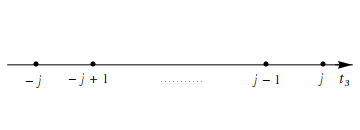
\includegraphics[width=200pt,keepaspectratio=true]{Addons/pesosu2}
\end{figure}
\pagebreak

Passiamo quindi a $SU(3)$. Dobbiamo innanzitutto trovare un insieme completo di operatori che commutano. Abbiamo immediatamente i due Casimir $F^{(2)}$ e $G^{(3)}$. Come lo completiamo? Siano $F_a$ i generatori di $SU(3)$ e definiamo:
\begin{align}
&F_{1,2,3}=T_{1,2,3} \notag\;, \\
&T_{\pm}=T_1\pm iT_2 \notag\;, \\
&V_{\pm}=F_4\pm iF_5 \notag\;, \\
&U_{\pm}=F_6\pm iF_7 \notag\;, \\
&Y=\frac{2}{\sqrt{3}}F_8\;.
\end{align}
Notiamo subito che $\{T_1,T_2,T_3\}$ generano un sottogruppo $SU(2)$ detto \emph{sottogruppo di T-spin}. Riscriviamo quindi l'algebra di $SU(3)$ in termini di questi nuovi operatori:
\begin{subequations}
\begin{equation}
[T_3,T_{\pm}]=\pm T_{\pm}\qquad [T_3,U_{\pm}]=\mp\frac{1}{2}U_{\pm}\qquad [T_3,V_{\pm}]=\pm\frac{1}{2}V_{\pm}\;,
\end{equation}
\begin{equation}
[Y,T_{\pm}]=0\qquad [Y,U_{\pm}]=\pm U_{\pm}\qquad [Y,V_{\pm}]=\pm V_{\pm}\;,
\end{equation}
\begin{equation}
[T_+,V_+]=0 \qquad [T_+,U_-]=0\qquad [U_+,V_+]=0\;,
\end{equation}
\begin{equation}
[T_+,V_-]=-U_-\qquad [T_+,U_+]=V_+\qquad [U_+,V_-]=T_-\qquad [T_3,Y]=0\;.
\end{equation}
\end{subequations}
Inoltre:
\begin{subequations}
\begin{align}
&[T_+,T_-]=2T_3\;, \\
&[U_+,U_-]=\frac{3}{2}Y-T_3\equiv 2U_3\;, \\
&[V_+,V_-]=\frac{3}{2}Y+T_3\equiv 2V_3\;,
\end{align}
\end{subequations}
Concludiamo perciò che esistono altri due sottogruppi $SU(2)$ generati da $\{V_1=F_4,V_2=F_5,V_3\}$ e $\{U_1=F_6,U_2=F_7,U_3\}$, detti rispettivamente \emph{sottogruppo di V-spin} e \emph{sottogruppo di U-spin}. \\
Possiamo adesso completare l'insieme completo di operatori prendendo $\{F^{(2)},G^{(3)},T^{(2)},T_3,Y\}$, dove $T^{(2)}$ è il Casimir quadratico del sottogruppo di $T$-spin. Allora le rappresentazioni irriducibili di $SU(3)$ saranno classificate da due indici, corrispondenti ai valori dei due Casimir di $SU(3)$. \\
Il diagramma peso di $SU(3)$ sarà dato quindi dal grafico bidimensionale in cui vengono riportati i valori degli operatori $T_3$ in ascissa e $Y$ in ordinata (v. figura):
\begin{figure}[h]
\centering
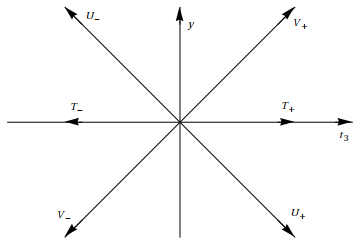
\includegraphics[width=200pt,keepaspectratio=true]{Addons/pesosu3}
\end{figure}

Gli effetti dei vari operatori definiti su un autostato simultaneo degli operatori di base sono i seguenti
\begin{itemize}
\item $T_+$ aumenta di $1/2$ il valore di $T_3$, mentre $T_-$ lo diminuisce di $1/2$;
\item $V_+$ aumenta di $1/2$ il valore di $T_3$ e di $1$ il valore di $Y$, mentre $V_-$ diminuisce di $1/2$ il valore di $T_3$ e di $1$ il valore di $Y$;
\item $U_+$ diminuisce di $1/2$ il valore di $T_3$ e aumenta di $1$ il valore di $Y$, mentre $U_-$ aumenta di $1/2$ il valore di $T_3$ e diminuisce di $1$ il valore di $Y$.
\end{itemize}
Data una rappresentazione $(p,q)$ irriducibile di $SU(3)$, il suo diagramma peso avrà struttura esagonale, con lati di lunghezza $p$ e $q$. In generale:
\begin{equation}
d(p,q)=\frac{1}{2}(p+1)(q+1)(p+q+2)\;.
\end{equation}
In analogia con $SU(2)$, definiamo uno stato di "peso massimo" $|\psi_{\mathrm{max}}\ket$ come lo stato avente $t_3$ massimo, che per una rappresentazione $(p,q)$ vale $t_3^{\mathrm{max}}=(p+q)/2$:
\begin{equation}
T_3|\psi_{\mathrm{max}}\ket=\frac{p+q}{2}|\psi_{\mathrm{max}}\ket\;.
\end{equation}
Inoltre si osserva che $|\psi_{\mathrm{max}}\ket$ appartiene a un multipletto di $U$-spin (con valore di $U_3$ minimo) e a un multipletto di $V$-spin (con valore di $V_3$ massimo):
\begin{subequations}
\begin{equation}
U_3|\psi_{\mathrm{max}}\ket=-\frac{q}{2}|\psi_{\mathrm{max}}\ket\;,
\end{equation}
\begin{equation}
V_3|\psi_{\mathrm{max}}\ket=\frac{p}{2}|\psi_{\mathrm{max}}\ket\;,
\end{equation}
\end{subequations}
con:
$$
T_+|\psi_{\mathrm{max}}\ket=V_+|\psi_{\mathrm{max}}\ket=U_-|\psi_{\mathrm{max}}\ket=0\;.
$$
Sommando le definizioni di $U_3,V_3$ otteniamo $Y=\dfrac{2}{3}(U_3+V_3)$. Da questa relazione possiamo trovare il valore di $Y$ su $|\psi_{\mathrm{max}}\ket$:
\begin{equation}
Y|\psi_{\mathrm{max}}\ket=\frac{2}{3}(U_3+V_3)|\psi_{\mathrm{max}}\ket=\frac{1}{3}(p-q)|\psi_{\mathrm{max}}\ket\;.
\end{equation}
Vogliamo infine valutare il Casimir quadratico su una rappresentazione irriducibile $(p,q)$:
$$
F^{(2)}_{(p,q)}=C_F^{(p,q)}\mathbb{I}_{d(p,q)\times d(p,q)}\;,
$$
cioè vogliamo determinare $C_F^{(p,q)}$. Per farlo, è sufficiente calcolare l'operatore sullo stato $|\psi_{\mathrm{max}}\ket$, scrivendolo come:
\begin{equation}
F^{(2)}_{(p,q)}=\frac{1}{2}\{T_+,T_-\}+\frac{1}{2}\{U_+,U_-\}+\frac{1}{2}\{V_+,V_-\}+T_3^2+\frac{3}{4}Y^2\;,
\end{equation}
e usando le relazioni trovare in precedenza. Il risultato è dato da:
\begin{equation}
C_F^{(p,q)}=\frac{1}{3}(p^2+pq+q^2)+(p+q)\;.
\end{equation}
Scriviamo adesso le rappresentazioni irriducibili di $SU(3)$ più semplici e i relativi diagrammi peso:
\begin{itemize}
\item $(p,q)=(0,0)$. Questa è la rappresentazione triviale, di dimensione $d(0,0)=1$ e diagramma peso:
\begin{figure}[h]
\centering
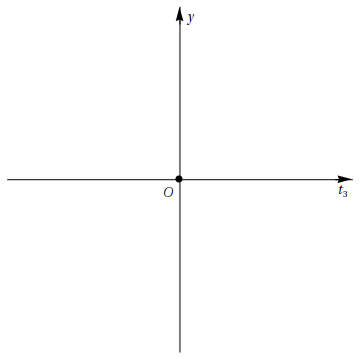
\includegraphics[width=150pt,keepaspectratio=true]{Addons/00}
\end{figure}
\pagebreak
\item $(p,q)=(1,0)$. Questa è la rappresentazione fondamentale di $SU(3)$, con dimensione $d(1,0)=3$. Il suo diagramma peso è:
\begin{figure}[h]
\centering
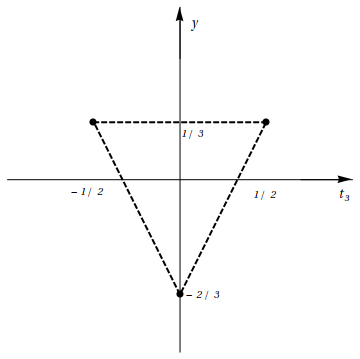
\includegraphics[width=200pt,keepaspectratio=true]{Addons/10}
\end{figure}

\item $(p,q)=(0,1)$. Questa è la rappresentazione complessa coniugata della fondamentale, e la sua dimensione è indicata con $d(0,1)=3^*$. Il suo diagramma peso si ottiene da quello della $(1,0)$ scambiando i segni in ordinata:
\begin{figure}[h]
\centering
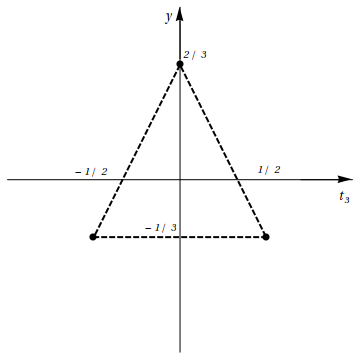
\includegraphics[width=200pt,keepaspectratio=true]{Addons/01}
\end{figure}

\item $(p,q)=(2,0)$. Questa rappresentazione ha dimensione $d(2,0)=6$. Il suo diagramma peso è:
\begin{figure}[h]
\centering
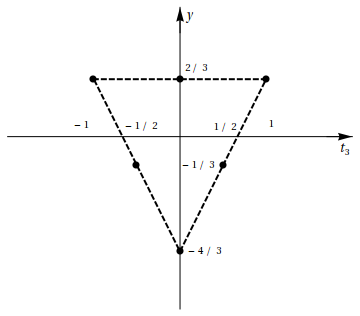
\includegraphics[width=200pt,keepaspectratio=true]{Addons/20}

\end{figure}
\pagebreak
\item $(p,q)=(0,2)$. Rappresentazione complessa coniugata di $(2,0)$, $d(0,2)=6^*$. Diagramma peso:
\begin{figure}[h]
\centering
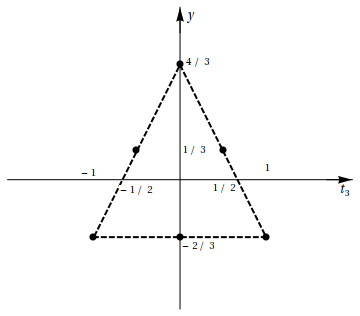
\includegraphics[width=200pt,keepaspectratio=true]{Addons/02}

\end{figure}
\cleardoublepage
\item $(p,q)=(1,1)$. Questa è la rappresentazione aggiunta, $d(1,1)=8$. Diagramma peso:
\begin{figure}[h]
\centering
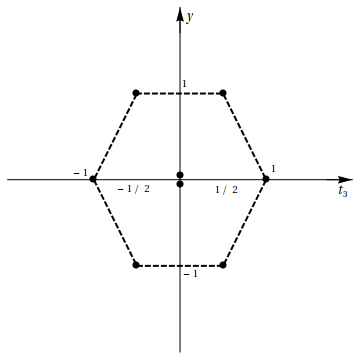
\includegraphics[width=200pt,keepaspectratio=true]{Addons/11}
\end{figure}
	
Lo stato con $(t_3,y)=(0,0)$ è doppiamente degenere. In un generico diagramma peso vale la seguente regola: lo strato più esterno è non degenere, quello immediatamente più interno è due volte degenere e così via. L'aumento della degenerazione si interrompe quando lo strato a cui si arriva ha una struttura triangolare.

\item $(p,q)=(3,0)$
\begin{figure}[h]
\centering
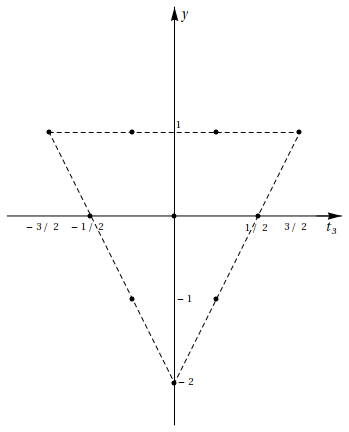
\includegraphics[width=200pt,keepaspectratio=true]{Addons/30}

\end{figure}
\pagebreak
\item $(p,q)=(2,1)$
\begin{figure}[h]
\centering
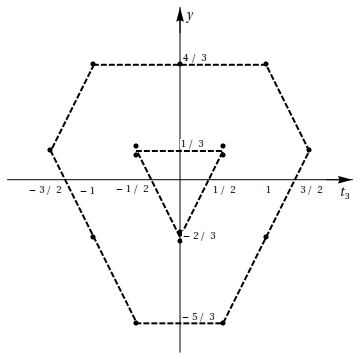
\includegraphics[width=200pt,keepaspectratio=true]{Addons/21}

\end{figure}

\end{itemize}
\subsection{Multipletti di spin isotopico}
Negli anni '60 le particelle conosciute, gli \emph{adroni}, si dividevano in due famiglie: i \emph{mesoni} (di spin intero) e i \emph{barioni} (di spin semi-intero). Era stato osservato che nelle interazioni forti il numero barionico $B$ si conservasse (ogni barione coinvolto nel processo da un $+1$, ogni antibarione un $-1$ e i mesoni $0$). All'epoca era nota una simmetria $SU(2)$ (spin isotopico) per le interazioni forti. I multipletti noti erano:
\begin{itemize}
\item $t=0$: 
\begin{align*}
&\eta,\eta',\omega,\phi &Q=t_3=0,B=0 \\
&\Lambda^0 &Q=t_3=0,B=1
\end{align*}
\item $t=1/2$:
\begin{align*}
&n,p & Q=t_3+\frac{1}{2},B=1 \\
& K^0,K^+ & Q=t_3+\frac{1}{2},B=0 \\
& K^-,\overline{K}^0 &Q=t_3-\frac{1}{2},B=0\\
& \Xi^-,\Xi^0 & Q=t_3-\frac{1}{2},B=1
\end{align*}
\item $t=1$:
\begin{align*}
&\pi^-,\pi^0,\pi^+ &Q=t_3,B=0 \\
&\rho^-,\rho^0,\rho^+ &Q=t_3,B=0 \\
&\Sigma^-,\Sigma^0,\Sigma^+ &Q=t_3,B=1
\end{align*}
\item $t=3/2$:
\begin{align*}
&\Delta^-,\Delta^0,\Delta^+,\Delta^{++} &Q=t_3+\frac{1}{2}
\end{align*}
\end{itemize}
Fu osservato che per molti multipletti di isospin vale la relazione $Q=t_3+B/2$. Quelli che non rispettavano questa regola vennero chiamati \emph{strani}. La relazione venne quindi corretta da Gell-Mann e Nishijima (1953):
\begin{equation}
\boxed{
Q=t_3+\frac{Y}{2}
},\qquad Y=B+S\;,
\end{equation}
dove $Y$ è l'\emph{ipercarica forte}, $B$ il numero barionico e $S$ la \emph{stranezza}. Questi numeri quantici si conservano nei processi forti. \\
I multipletti di isospin possono quindi essere "graficamente impilati", ottenendo alcune rappresentazioni irriducibili di $SU(3)$. Questa osservazione fece pensare che la simmetria $SU(2)$ di isospin poteva essere generalizzata ad una simmetria approssimata $SU(3)$ di \emph{sapore} (\emph{flavor}). Questa è una simmetria peggiore, in quanto le differenze di massa all'interno dei multipletti di flavor sono più consistenti rispetto a quelle tipiche dell'isospin. Questa impilazione aiutò a predirre l'esistenza di un barione con $J^P=\frac{3}{2}^+,Y=-2,S=-3$ che andava a completare il diagramma peso del decupletto barionico, ossia l'$\Omega^-$ (che all'epoca non era ancora noto). Fu inoltre osservato che tutte le componenti di un multipletto di $U$-spin hanno la stessa carica.
\subsection{Rappresentazione complessa coniugata in $SU(N)$}
Data una certa rappresentazione di $SU(N)$, $U=\exp(i\epsilon_aF_a)$, con $[F_a,F_b]=if_{abc}F_c$, prendiamone il complesso coniugato (l'operazione preserva la struttura di gruppo):
$$
U^*=e^{-i\epsilon_aF_a^*}=e^{i\epsilon_a\hat{F}_a}\;,
$$
dove $\hat{F}_a\equiv -F_a^*$ soddisfano l'algebra di Lie: $[\hat{F}_a,\hat{F}_b]=if_{abc}\hat{F}_c$.
\begin{dfn}
$U$ e $U^*$ si dicono \emph{equivalenti} se esiste una matrice $S$ invertibile tale che $SUS^{-1}=U^*$ per ogni $U\in SU(N)$. In termini dei generatori:
$$
SUS^{-1}=Se^{i\epsilon_aF_a}S^{-1}=e^{i\epsilon_aSF_aS^{-1}}=U^*=e^{i\epsilon_a\hat{F}_a}\qquad \forall \epsilon_a\;,
$$
da cui la condizione di equivalenza sui generatori si legge come $SF_aS^{-1}=\hat{F}_a=-F_a^*$.
\end{dfn}
\begin{exm}
Consideriamo la rappresentazione fondamentale di $SU(2)$, $F_a=\sigma_a/2$. Si ha $\sigma_2\sigma_a\sigma_2=-\sigma_a^*$ (cioè $S=\sigma_2$), quindi la rappresentazione fondamentale e la sua complessa coniugata sono equivalenti. Per $SU(3)$ invece questo non è vero.
\end{exm}
\begin{thm} 
Se una data rappresentazione hermitiana è reale (cioè è equivalente alla sua complessa coniugata), allora i generatori hanno autovalori in coppie di segno opposto.

\end{thm}
\begin{exm} 
Consideriamo la rappresentazione fondamentale di $SU(3)$ e il generatore $\lambda_8$, dato da:
\begin{equation*}
\lambda_8=\frac{1}{\sqrt{3}}\left(\begin{matrix}
1 & 0 & 0 \\
0 & 1 & 0 \\
0 & 0 & -2
\end{matrix}\right)\;.
\end{equation*}
Questo non rispetta la condizione sugli autovalori, e quindi la rappresentazione non è reale.
\end{exm}
\begin{exm}
La rappresentazone aggiunta di $SU(N)$ è reale, infatti $\hat{F}_a^{(\mathrm{agg})}=-(F^{(\mathrm{agg})}_a)^*=F_a$.
\end{exm}
\proof 
Per ipotesi $SF_aS^{-1}=-F_a^*$ per ipotesi. Sia $|\lambda\ket$ un autostato di $F_a$, i.e. $F_a|\lambda\ket=\lambda|\lambda\ket$, con $\lambda\in\mathbb{R}$ perché $F_a$ è hermitiano. Allora:
$$
F_a^*S|\lambda\ket=-(SF_aS^{-1})S|\lambda\ket=-SF_a|\lambda\ket=-\lambda S|\lambda\ket\;.
$$
Coniugando questa relazione si ottiene:
$$
F_a(S|\lambda\ket)^*=-\lambda(S|\lambda\ket)^*
$$
cioè $(S|\lambda\ket)^*$ è autostato di $F_a$ per $-\lambda$.
\endproof

Le particelle note all'epoca di Gell-Mann non si disponevano nella rappresentazione fondamentale di $SU(3)$. Questa peculiarità fece sorgere il dubbio che dovessero esistere particelle fondamentali che occupavano la rappresentazione $(1,0)$, i \emph{quarks}, i cui stati legati costituivano le particelle adroniche osservate.
\cleardoublepage
\section{Prodotto diretto di rappresentazioni irriducibili di $SU(3)$}
\begin{exm}
In $SU(2)$ consideriamo due particelle di spin $J_1,J_2$: lo stato complessivo trasforma sotto rotazioni come il prodotto diretto delle due rappresentazioni, i.e.:
$$
\mathcal{D}^{(J_1)}_{M_1 M_1'}(R)\mathcal{D}^{(J_2)}_{M_2 M_2'}(R)\;.
$$
Per $SU(2)$ il prodotto diretto si può scrivere in termini della \emph{serie di Clebsch-Gordan}:
\begin{equation}
\mathcal{D}^{(J_1)}_{M_1 M_1'}(R)\mathcal{D}^{(J_2)}_{M_2 M_2'}(R)=\sum_{J=|J_1-J_2|}^{J_1+J_2}\sum_M\sum_{M'}C_{M_1M_2M}^{J_1J_2J}C_{M_1'M_2'M}^{J_1J_2J}\mathcal{D}^{(J)}_{MM'}(R)\;.
\end{equation}
Se non si è interessati ai particolari coefficienti, il risultato si può ottenere con il metodo grafico, sfruttando l'additività di $J_z$.
\end{exm}

Il metodo grafico può essere esteso a $SU(3)$, in cui stavolta sfruttiamo l'additività di $y$ e $t_3$\footnote{Non sarà riportato qui perché i grafici sono difficili da gestire.}.
\subsection{Metodo tensoriale}
\begin{dfn} 
\begin{enumerate}
\item Un vettore \emph{controvariante} $q^i$ è un oggetto che trasforma sotto $SU(N)$ come:
\begin{equation}
q^i\longrightarrow q'^i=U_{ij}q^j\equiv U^i_jq^j\;,
\end{equation}
con $U$ in rappresentazione fondamentale di $SU(N)$;
\item un vettore \emph{covariante} $\overline{q}_i$ è un oggetto che trasforma sotto $SU(N)$ come:
\begin{equation}
\overline{q}_i\longrightarrow \overline{q}'_i=U^*_{ij}\overline{q}_j=(\adj{U})_{ij}\overline{q}_j\equiv (\adj{U})^j_i\overline{q}_j\;,
\end{equation}
con $U^*$ in rappresentazione complessa coniugata della fondamentale di $SU(N)$;
\item un \emph{tensore (misto) di rango} $(p,q)$ $T^{i_1\cdots i_p}_{j_1\cdots j_q}$ trasforma sotto $SU(N)$ come:
\begin{equation}
T^{i_1\cdots i_p}_{j_1\cdots j_q}\longrightarrow T'^{i_1\cdots i_p}_{j_1\cdots j_q}=U^{i_1}_{\alpha_1}\cdots U^{i_p}_{\alpha_p}(\adj{U})^{\beta_1}_{j_1}\cdots (\adj{U})^{\beta_q}_{j_q}T^{\alpha_1\cdots \alpha_p}_{\beta_1\cdots\beta_q}\;,
\end{equation}
cioè trasforma come il prodotto di $p$ rappresentazioni fondamentali e $q$ rappresentazioni antifondamentali;
\item la \emph{delta di Kroenecker} è un tensore invariante per $SU(N)$:
\begin{equation}
\delta^i_j=\begin{cases}
1\qquad i=j \\
0\qquad i\ne j
\end{cases}\;;
\end{equation}
infatti $\delta^i_j\longrightarrow\delta'^i_j=U^i_{\alpha}(\adj{U})^{\beta}_j\delta^{\alpha}_{\beta}=(U\adj{U})^i_j=\delta^i_j$. Anche il \emph{tensore completamente antisimmetrico}:
\begin{equation}
\epsilon^{i_1\cdots i_N}=\epsilon_{i_1\cdots i_N}=\begin{cases}
+1\quad \mbox{se}\; (i_1,\ldots,i_N)\;\mbox{è una permutazione pari di}\; (1,\ldots,N) \\
-1\quad \mbox{se}\; (i_1,\ldots,i_N)\;\mbox{è una permutazione dispari di}\; (1,\ldots,N) \\
0\quad \mbox{altrimenti (almeno due indici uguali)}
\end{cases}\;,
\end{equation}
è invariante sotto $SU(N)$:
\begin{equation}
\epsilon'^{i_1\cdots i_N}=U^{i_1}_{\alpha_1}\cdots U^{i_N}_{\alpha_N}\epsilon^{\alpha_1\cdots\alpha_N}=\det U\epsilon^{i_1\cdots i_N}=\epsilon^{i_1\cdots i_N}\;,
\end{equation}
in quanto $\det U=1$;
\item la \emph{traccia} di un tensore su una coppia di indici è data da:
\begin{equation}
T^{\alpha i_2\cdots i_p}_{\alpha j_2\cdots j_q}=T^{i_1\cdots i_p}_{j_1\cdots j_p}\delta^{j_1}_{i_1}\;.
\end{equation}
\end{enumerate}
\end{dfn}
Abbandoniamo adesso il caso generale e focalizziamoci su $SU(3)$. Un tensore $T^{i_1\cdots i_p}_{j_1\cdots j_q}$ di rango $(p,q)$ avrà in generale $3^{p+q}$ componenti.
\subsection{Riduzione di un tensore di rango $(p,q)$}
Definiamo tre operazioni di riduzione di un tensore.
\begin{enumerate}
\item Contrazione di un indice controvariante e uno covariante tramite la delta di Kroenecker:
$$
T^{i_1\cdots i_p}_{j_1\cdots j_q}\delta^{j_a}_{i_b}\;.
$$
Il tensore risultante avrà rango $(p-1,q-1)$.
\item Contrazione su due indici covarianti tramite il tensore completamente antisimmetrico:
$$
T^{i_1\cdots i_p}_{j_1\cdots j_q}\epsilon^{j_aj_bi_{p+1}}\;.
$$
Il tensore risultante avrà rango $(p+1,q-2)$.
\item Contrazione su due indici controvarianti tramite il tensore completamente antisimmetrico:
$$
T^{i_1\cdots i_p}_{j_1\cdots j_q}\epsilon_{i_ai_bj_{q+1}}\;.
$$
Il tensore risultante avrà rango $(p-2,q+1)$.
\end{enumerate}
\begin{dfn}
Un tensore $T$ di rango $(p,q)$ si dice \emph{irriducibile} se, tramite le operazioni di riduzione (1),(2),(3), si ottiene sempre il tensore identicamente nullo. Altrimenti, il tensore è detto \emph{riducibile}.
\end{dfn}
\begin{thm}
Sia $T$ un tensore di rango $(p,q)$ e siano $\phi_1,\ldots,\phi_d$ le componenti linearmente indipendenti di $T$. Se le incolonniamo in un vettore e trasformiamo sotto $SU(N)$ $T$ in $T'$, avremo una trasformazione indotta:
\begin{equation}
\left(\begin{matrix}
\phi_1 \\
\vdots \\
\phi_d
\end{matrix}\right)\longrightarrow\left(\begin{matrix}
\phi_1'\\
\vdots \\
\phi_d'
\end{matrix}\right)=V_{d\times d}\left(\begin{matrix}
\phi_1 \\
\vdots \\
\phi_d
\end{matrix}\right)\;,
\end{equation}
con $V_{d\times d}$ rappresentazione di $SU(3)$ di dimensione $d$. Allora $V_{d\times d}$ è irriducibile se $T$ è irriducibile.
\end{thm}
I tensori $c\delta^i_j$, $c\epsilon^{ijk}$, $c\epsilon_{ijk}$ ($c$ costante) sono invarianti, e quindi irriducibili. Corrispondono alla rappresentazione irriducibile $(0,0)=\mathbf{1}$. Un generico tensore di rango $(p,q)$ sarà irriducibile se e solo se è simmetrico sugli indici controvarianti e sugli indici covarianti, così che le contrazioni con il tensore completamente antisimmetrico siano nulle, ed è a traccia nulla, così che la contrazione con la delta sia nulla. \\
Il numero di componenti linearmente indipendenti di un tensore irriducibile di rango $(p,q)$ e $d(p,q)=\frac{1}{2}(p+1)(q+1)(p+q+2)$. Quindi le componenti indipendenti di un tensore irriducibile di rango $(p,q)$ trasformano sotto $SU(3)$ come la rappresentazione irriducibile $(p,q)$.
\begin{table}[h]
\centering
\begin{tabular}{c|c|l}
\toprule
$(p,q)$ & $d(p,q)$ & tensore irriducibile \\
\midrule
$(0,0)$ & $\mathbf{1}$ & $\mathbb{I}$ \\
$(1,0)$ & $\mathbf{3}$ & $q^i$ \\
$(0,1)$ & $\mathbf{3}^*$ & $\overline{q}_i$ \\
$(2,0)$ & $\mathbf{6}$ & $S^{ij}$ (simmetrico) \\
$(0,2)$ & $\mathbf{6}^*$ & $S_{ij}$ (simmetrico) \\
$(1,1)$ & $\mathbf{8}$ &  $T^i_j$ (traceless) \\
$(3,0)$ & $\mathbf{10}$ & $S^{ijk}$ (completamente simmetrico) \\
$(0,3)$ & $\mathbf{10}^*$ & $S_{ijk}$ (completamente simmetrico) \\
$(2,1)$ & $\mathbf{15}$ & $S^{ij}_k$ (simmetrico negli indici in altro e traceless) \\
\bottomrule
\end{tabular}
\end{table}
\subsection{Decomposizione del prodotto diretto con il metodo tensoriale}
\begin{exm}
Prendiamo un tensore riducibile di rango $(2,0)$ $T^{ij}$. Possiamo decomporlo in somma di tensore irriducibili:
\begin{equation}
T^{ij}=\frac{1}{2}(T^{ij}+T^{ji})+\frac{1}{2}(T^{ij}-T^{ij})\equiv S^{ij}+A^{ij}\;,
\end{equation}
con  $S^{ij}=S^{ji}$, quindi $S^{ij}\in \mathbf{6}$ ed è irriducibile. Quello che resta è una $\mathbf{3}$ oppure una  $\mathbf{3}^*$? Eseguiamo la riduzione:
$$
\overline{q}_k\equiv \epsilon_{ijk}T^{ij}=\epsilon_{ijk}(S^{ij}+A^{ij})=\epsilon_{ijk}A^{ij}\;,
$$
con $\overline{q}_k\in\mathbf{3}^*$. Calcoliamo adesso:
$$
\epsilon^{ijk}\overline{q}_k=\epsilon^{ijk}\epsilon_{abk}T^{ab}=(\delta^i_a\delta^j_b-\delta^i_b\delta^j_a)T^{ab}=T^{ij}-T^{ji}=2A^{ij}\;,
$$
cioè:
$$
A^{ij}=\frac{1}{2}\epsilon^{ijk}\overline{q}_k\;,
$$
da cui:
\begin{equation}
T^{ij}=S^{ij}+\frac{1}{2}\epsilon^{ijk}\overline{q}_k\;,
\end{equation}
cioè $\mathbf{3}\otimes\mathbf{3}=\mathbf{6}\oplus \mathbf{3}^*$. Notiamo che la decomposizione in parte simmetrica e antisimmetrica è invariante sotto $SU(3)$.
\end{exm}
\begin{exm} 
Sia $T^i_j\in \mathbf{3}\otimes \mathbf{3}^*$. In generale avremo 9 componenti. Per avere un tensore irriducibile manca la condizione di traccia nulla. Allora possiamo decomporre come:
\begin{equation}
T^i_j=\left(T^i_j-\frac{1}{3}T^k_k\delta^i_j\right)+\frac{1}{3}T^k_k\delta^i_j\equiv\hat{T}^i_j+\frac{1}{3}T^k_k\delta^i_j\;,
\end{equation}
adesso $\hat{T}^i_j$ è a traccia nulla, e quindi irriducibile, cioè $\hat{T}^i_j\in \mathbf{8}$. Il resto è proporzionale al tensore invariante $\delta^i_j$, quindi concludiamo che $\mathbf{3}\otimes\mathbf{3}^*=\mathbf{8}\oplus\mathbf{1}$.
\end{exm}
Vale inoltre la seguente relazione: se $T^{i_1\cdots i_p}_{j_1\cdots j_q}$ è un tensore irriducibile di rango $(p,q)$ e $S^{i_1\cdots i_q}_{j_1\cdots j_p}$ è un tensore irriducibile di rango $(q,p)$, allora le componenti di $T$ trasformano come le componenti di $S^*$, cioè $(p,q)=(q,p)^*$.
\cleardoublepage
\section{Modello a quarks}
Proposto nel 1964 da Gell-Mann e Zweig, il modello introduce delle particelle fondamentali dette quarks che popolano la rappresentazione fondamentale di $SU(3)$. I quarks si presentano in tre \emph{flavors}: $u$ (\emph{up}), $d$ (\emph{down}), $s$ (\emph{strange}). Le corrispondenti antiparticelle popolano la rappresentazione complessa coniugata della fondamentale. I numeri quantici di questi tra quarks sono riassunti nella seguente tabella:
\begin{table}[h]
\centering
\begin{tabular}{c|c|c|c|c|c|c}
\toprule
flavor & $t$ & $t_3$ & $y$ & $Q=t_3+y/2$ & $B$ & $S$ \\
\midrule
$u$ & $1/2$ & $1/2$ & $1/3$ & $2/3$ & $1/3$ & 0 \\
$d$ & $1/2$ & $-1/2$ & $1/3$ & $-1/3$ & $1/3$ & 0 \\
$s$ & $0$ & $0$ & $-2/3$ & $-1/3$ & $1/3$ & $-1$\\
\midrule
\end{tabular}
\end{table}

I mesoni e i barioni sono quindi stati legati di questi quarks: i mesoni, aventi spin intero, saranno formati da una coppia quark-antiquark, mentre i barioni, di spin semi-intero saranno formati da tre quark. La simmetria $SU(2)$ di isospin coinvolge solo i quarks $u,d$. \\

\textbf{Paradossi del modello a quarks} \\
\begin{enumerate}
\item Non sono mai stati osservati i quarks, né stati legati $qq$ oppure $qq\overline{q}$,$qqqq$, etc...
\item Problemi con la statistica di Fermi-Dirac: lo stato $|\Delta^{++},J=3/2\ket=|u_{(1)}^{\uparrow}u_{(2)}^{\uparrow}u_{(3)}^{\uparrow}\ket_{\ell=0}$ è completamente simmetrico (spin, orbitale e flavor), quando in realtà dovrebbe essere completamente antisimmetrico (in quanto stato legato di tre fermioni identici).
\end{enumerate}
Entrambi i paradossi furono risolti con la cosiddetta \textbf{proposta del colore}: per rendere antisimmetrico lo stato di cui sopra fu proposto un numero quantico aggiuntivo detto appunto \emph{colore}. Per ogni flavor, si hanno tre colori:
\begin{align*}
&u^i=(u^1,u^2,u^3)\;, \\
&d^i=(d^1,d^2,d^3)\;, \\
&s^i=(s^1,s^2,s^3)\;.
\end{align*}
Usando il colore, possiamo facilmente antisimmetrizzare $|\Delta^{++}\ket$:
\begin{equation}
|\Delta^{++},J=3/2\ket=\frac{1}{\sqrt{3!}}\epsilon_{ijk}|u^i_{(1)}\uparrow,u^j_{(2)}\uparrow,u^k_{(3)}\uparrow\ket_{\ell=0}\;.
\end{equation}
L'introduzione del numero quantico di colore mette in luce una nuova simmetria: \\
\textbf{Simmetria $SU(3)$ di colore}
$$
u^i\longrightarrow u'^i=U^i_ju^j\;,
$$
con $U^i_j\in SU(3)_C$ (mescola le componenti di colore). Applicando una trasformazione $SU(3)_C$ allo stato $|\Delta^{++}\ket$ si ottiene:
$$
\epsilon_{ijk}u'^iu'^ju'^k=\epsilon_{ijk}U^i_aU^j_bU^k_cu^au^bu^c=\det U\epsilon_{abc}u^au^bu^c=\epsilon_{abc}u^au^bu^c\;.
$$
Quindi lo stato $|\Delta^{++}\ket$ è invariante per trasformazioni $SU(3)_C$, in particolare, è un \emph{singoletto} di colore. Il discorso viene esteso a tutti gli stati adronici tramite il \\
\textbf{Postulato del confinamento:} tutti gli stati adronici (e le corrispondenti osservabili fisiche) sono \emph{singoletti di colore}. \\
Per i mesoni, si postula che gli stati $|q_i\overline{q}_j\ket$ (a priori 9 stati di colore) siano singoletti di colore dati dalla contrazione tra gli indici $i,j$:
$$
|q^i\overline{q}_j\ket\longrightarrow\frac{1}{\sqrt{3}}\sum_{i=1}^3|q^i\overline{q}_i\ket\;.
$$
Notiamo che i $q^i$ trasformano secondo la rappresentazione $\mathbf{3}_C$, mentre i $\overline{q}_i$ secondo la $\mathbf{3}^*_C$, cioè:
\begin{align}
&q^i\longrightarrow q'^i=U^i_jq^j \notag\;, \\
&\overline{q}_i\longrightarrow \overline{q}'_i=(\adj{U})^j_i\overline{q}_j\;.
\end{align}
Estendendo quello che abbiamo ricavato sui prodotti diretti si hanno le seguenti relazioni:
\begin{align}
&\mathbf{3}_C\otimes\mathbf{3}^*_C=\mathbf{1}_C\oplus\mathbf{8}_C\;, \notag \\
&\mathbf{3}_C\otimes\mathbf{3}_C\otimes\mathbf{3}_C=\mathbf{1}_C\oplus\mathbf{8}_C\oplus\mathbf{8}_C\oplus\mathbf{10}_C\;.
\end{align}
Per il postulato del confinamento, in natura si realizza solo la rappresentazione $\mathbf{1}_C$.
\subsection{Evidenze sperimentali (indirette) del numero quantico di colore}
\begin{enumerate}
\item Decadimento $\pi^0\to \gamma\gamma$. Si può mostrare che la larghezza di decadimento del processo è:
\begin{equation}
\Gamma(\pi^o\to\gamma\gamma)=N_C^2(Q_u^2-Q_d^2)\frac{\alpha^2m_{\pi}^3}{64\pi^3F_{\pi}^2}=\left(\frac{N_C}{3}\right)^2\frac{\alpha^2m_{\pi}^3}{64\pi^3F_{\pi}^2}\approx N_C^2\times 0.84\;\mathrm{eV}\;,
\end{equation}
dove $N_C$ è il numero di colori, $Q_u$ e $Q_d$ sono rispettivamente la carica del quark up e del down, $\alpha\approx 1/137$ è la costante di struttura fine, $m_{\pi}\approx 135$ MeV, $F_{\pi}\approx 92$ MeV è la costante di decadimento del $\pi^0$. Confrontando con il valore sperimentale della larghezza $\Gamma_{\mathrm{exp}}\approx 7.48$ eV, si ha perfetto accordo per $N_C=3$.
\item Annichilazione $e^-e^+\to$ adroni. Si suppone che alla base di questo processo vi sia un processo fondamentale $e^-e^+\to q\overline{q}\to$ (adronizzazione) $\to$ adroni. Ad \emph{alte energie} si osserva che:
\begin{equation}
\sigma(e^-e^+\to\mbox{adroni})\approx \sum_{f,i}\sigma(e^-e^+\to \overline{q}_f^i\overline{q}_{f,i})\;,
\end{equation}
con $f=1,\ldots, N_f(s)$ numero di flavors che possono contribuire al processo ($\sqrt{s}$ è l'energia nel sistema del centro di massa), cioè i flavors tali che $2m_f<\sqrt{s}$, e $i=1,\ldots,N_c$ è il numero di colori. \\
\textbf{N.B.} La carica dei quark dipende dal flavor e non dal colore:
$$
\lag_{I}^{\mathrm{e.m.}}=-\sum_{i=1}^{N_f}Q_f|e|\sum_{i=1}^{N_c}\overline{\psi}_i\gamma^{\mu}\psi_iA_{\mu}\;.
$$
Quindi la corrente elettromagnetica è invariante per $SU(N_c)$, in particolare è un singoletto di colore (in accordo con il postulato del confinamento). Allora la corrente e.m. avrà una simmetria $U(1)_{\mathrm{e.m.}}\times SU(N_c)_c$. \\

Nel limite $s\gg m_f^2,m_e^2$ la sezione d'urto differenziale, mediata sulle polarizzazioni iniziali e sommata su quelle finali sarà data da:
\begin{equation}
\dev{\sigma}{\Omega}(e^+e^-\to q_f^i\overline{q}_{f,i})\simeq \frac{\alpha^2}{4s}Q_f^2(1+\cos^2\theta)\;,
\end{equation}
da cui:
\begin{equation}
\sigma(e^+e^-\to q_f^i\overline{q}_{f,i})\simeq \frac{4\pi\alpha^2}{3s}Q_f^2\;.
\end{equation}
Si definisce quindi il \emph{rapporto R} (o rapporto di Drell) come:
\begin{equation}
R=\frac{\sigma(e^+e^-\to\mbox{adroni})}{\sigma(e^+e^-\to\mu^+\mu^-)}\simeq N_c\sum_{f=1}^{N_f(s)}Q_f^2\;.
\end{equation}
Sperimentalmente, si osserva che la dipendenza di $R$ da $\sqrt{s}$ è costante e vale circa $2$ fino a energie di 3 GeV. Tra 3 e 4 GeV si hanno delle risonanze, dopodiché il valore di $R$ rimane costante fino a 9 GeV e vale $10/3=2+4/3$. Tra 9 e 10 GeV si hanno altre risonanze, e poi di nuovo costanza a $11/3=2+4/3+1/3$. Le risonanze furono spiegate con l'attivazione dei canali per dei nuovi quarks che contribuiscono alla sezione d'urto. Tra 3 e 4 GeV si apre il canale del quark \emph{charm} ($c$). Il 4/3 di differenza rappresenta la carica al quadrato del $c$ moltiplicata per il suo $N_c$. Si ottiene quindi $Q_c=2/3,N_c=3, m_c\approx 1.5$ GeV. Tra 9 e 10 GeV si apre il canale del quark \emph{bottom} ($b$). Con gli stessi ragionamenti si ottiene $Q_b=-1/3, m_b\approx 4.5$ GeV. L'accordo tra esperimento e teoria si ha, ad alte energie, per $N_c=3$.
\end{enumerate}
\cleardoublepage
\section{Teoria di campo quantistica per i quarks (QCD)}
\begin{exm}[QED]
Fermioni di spin $1/2$ e carica $q=Q|e|$. La Lagrangiana è:
\begin{equation}
\lag=\overline{\psi}(i\slashed{D}-m)\psi-\frac{1}{4}F_{\mu\nu}F^{\mu\nu}=\lag_F+\lag_G\;,
\end{equation}
con $\slashed{D}=\gamma^{\mu}D_{\mu}$ e $D_{\mu}=\partial_{\mu}+iQ|e|A_{\mu}$. Concentriamoci inizialmente sulla parte fermionica:
$$
\lag_F=\overline{\psi}(i\slashed{D}-m)\psi=\overline{\psi}(i\slashed{\partial}-m)\psi-Q|e|\overline{\psi}\slashed{A}\psi\equiv \lag_0+\lag_I\;.
$$
$\lag_0,\lag_I,\lag_F,\lag_G$ sono invarianti per \emph{trasformazioni di gauge $U(1)$ globali}:
\begin{align}
&\psi(x)\to \psi'(x)=e^{iQ\theta}\psi(x)\qquad (\theta=\mbox{cost.}) \notag\;, \\
& A_{\mu}(x)\to A_{\mu}(x)\;,
\end{align}
mentre $\lag_F,\lag_G$ sono invarianti anche per \emph{trasformazioni di gauge $U(1)$ locali}:
\begin{align}
&\psi(x)\to \psi'(x)=e^{iQ\theta(x)}\psi(x) \notag\;, \\
&A_{\mu}(x)\to A_{\mu}'(x)=A_{\mu}(x)-\frac{1}{|e|}\partial_{\mu}\theta(x)\;.
\end{align}
$D_{\mu}$ è detta \emph{derivata covariante} perché trasforma come $\psi$ sotto trasformazioni locali:
\begin{align*}
D_{\mu}\psi(x)\to D_{\mu}'\psi'(x) &=(\partial_{\mu}+i|e|QA_{\mu}'(x))\psi(x)=e^{iQ\theta}(\partial_{\mu}\psi+iQ(\partial_{\mu}\theta)\psi+iQ|e|A_{\mu}\psi-iQ(\partial_{\mu}\theta)\psi) \notag \\
&= e^{iQ\theta(x)}(\partial_{\mu}+iQ|e|A_{\mu})\psi=e^{iQ\theta(x)}D_{\mu}\psi\;,
\end{align*}
da cui $D_{\mu}'\psi'=e^{iQ\theta(x)}D_{\mu}\psi=e^{iQ\theta(x)}D_{\mu}e^{-iQ\theta(x)}\psi'$, cioè l'operatore $D_{\mu}$ trasforma come:
\begin{equation}
D_{\mu}\to D_{\mu}'=e^{iQ\theta(x)}D_{\mu}e^{-iQ\theta(x)}\;.
\end{equation}
\textbf{Tensore intensità di campo.} \\
Consideriamo la quantità $[D_{\mu},D_{\nu}]\psi=[(\partial_{\mu}+iQ|e|A_{\mu}),(\partial_{\nu}+iQ|e|A_{\nu})]\psi$. Nel caso abeliano della QED, rimangono solo i termini misti perché $A_{\mu}$ commuta con se stesso, quindi:
\begin{align*}
[D_{\mu},D_{\nu}]\psi &= iQ|e|\left([\partial_{\mu},A_{\nu}]+[A_{\mu},\partial_{\nu}]\right)\psi \\
&= iQ|e|(\partial_{\mu}(A_{\nu}\psi)-A_{\nu}\partial_{\mu}\psi+A_{\mu}\partial_{\nu}\psi-\partial_{\nu}(A_{\mu}\psi)) \\
&= iQ|e|\left((\partial_{\mu}A_{\nu})\psi+A_{\nu}\partial_{\mu}\psi-A_{\nu}\partial_{\mu}\psi+A_{\mu}\partial_{\nu}\psi-(\partial_{\nu}A_{\mu})\psi-A_{\mu}\partial_{\nu}\psi\right) \\
&= iQ|e|(\partial_{\mu}A_{\nu}-\partial_{\nu}A_{\mu})\psi\equiv iQ|e|F_{\mu\nu}\psi\;,
\end{align*}
cioè $F_{\mu\nu}\equiv [D_{\mu},D_{\nu}]$.
\end{exm} $ \\ $
Passiamo adesso al caso non abeliano di $SU(N_c)$. Abbiamo:
\begin{equation}
\lag_0=\sum_{i=1}^{N_c}\overline{\psi}_i(i\slashed{\partial}-m)\psi_i\;,
\end{equation}
con $m$ uguale per tutti i colori. Definiamo:
\begin{equation}
\psi=\left(\begin{matrix}
\psi_1 \\
\vdots \\
\psi_{N_c}
\end{matrix}\right)\;.
\end{equation}
Allora la Lagrangiana libera sarà:
\begin{equation}
\lag_0=\overline{\psi}(i\slashed{\partial}-m)\psi\;.
\end{equation}
Abbiamo una simmetria globale $SU(N_c)$:
\begin{align}
&\psi\to \psi'=U\psi \notag\;, \\
&\overline{\psi}\to\overline{\psi}'=\overline{\psi}\adj{U}\;,
\end{align}
con $U\in SU(N_c)$. Le $\psi$ trasformano come la rappresentazione fondamentale di $SU(N_c)$ (perché hanno proprio $N_c$ componenti), quindi (indichiamo con $T_a$ i generatori nella rappresentazione fondamentale):
\begin{align}
&U=\exp\left(i\sum_{a=1}^{N_c^2-1}\theta_aT_a\right) \notag\;, \\
&[T_a,T_b]=if_{abc}T_c \notag\;, \\
&\tr[T_aT_b]=\frac{1}{2}\delta_{ab}\;.
\end{align}
Vogliamo quindi passare al caso locale: $\lag_0$ non sarà più invariante a causa del termine cinetico. Per generalizzare la simmetria dobbiamo allora aggiungere a $\lag_0$ un termine di interazione di tipo accoppiamento minimale (come nel caso della QED): $\lag_0\to \lag_0+\lag_I\equiv\lag_F$.
\subsection{Trasporto parallelo}
\begin{dfn}
Sia $\psi\in V_x$ un vettore. Definiamo il \emph{trasporto parallelo} lungo una curva $C_{y\leftarrow x}$ come una trasformazione $W(C_{y\leftarrow x}):V_x\to V_y$, $W(C_{y\leftarrow x})\in SU(N_c)$, con le seguenti proprietà:
\begin{enumerate}
\item $W(0)=\mathbb{I}$ (dove $0$ indica una curva di lunghezza nulla);
\item $W(C_2\circ C_1)=W(C_2)W(C_1)$;
\item $W(-C)=W(C)^{-1}$;
\item sotto una trasformazione di gauge locale:
\begin{align*}
&\psi(x)\to\psi'(x)=U(x)\psi(x)\;, \\
&\psi(y)\to\psi'(y)=U(y)\psi(y)\;,
\end{align*}
si abbia $W(C_{y\leftarrow x})\to W'(C_{y\leftarrow x})=U(y)W(C_{y\leftarrow x})\adj{U}(x)$. In questo modo, se $\stackrel{\sim}{\psi}(y)\equiv W(C_{y\leftarrow x})\psi(x)$ allora:
$$
\stackrel{\sim}{\psi'}(y)=W'(C_{y\leftarrow x})\psi'(x)=U(y)W(C_{y\leftarrow x})\adj{U}(x)U(x)\psi(x)=U(y)\stackrel{\sim}{\psi}(y)\;.
$$
\end{enumerate}
\end{dfn}
\subsection{Campi di gauge}
Consideriamo il trasporto parallelo infinitesimo da $x$ a $x+\diff{x}$:
\begin{equation}
W(C_{x+\diff{x}\leftarrow x})\equiv \exp(-igA_{\mu}(x)\diff{x}^{\mu})\simeq 1-igA_{\mu}(x)\diff{x}^{\mu}\;,
\end{equation}
con $A_{\mu}(x)\in su(N_c)$ (algebra di $SU(N_c)$), cioè tale che $\adj{A}_{\mu}=A_{\mu}$ e $\tr A_{\mu}=0$, quindi scrivibile in termini dei generatori:
\begin{equation}
A_{\mu}(x)=\sum_{a=1}^{N_c^2-1}A_{\mu}^aT_a\;.
\end{equation}
Gli $A_{\mu}^a$ sono detti \emph{campi di gauge}. Vediamo come trasformano gli $A_{\mu}(x)$ sotto trasformazione di gauge:
\begin{align*}
W'(C_{x+\diff{x}\leftarrow x})=1-igA_{\mu}'(x)\diff{x}^{\mu} &= U(x+\diff{x})W(C_{x+\diff{x}\leftarrow x})\adj{U}(x) \\
&= U(x+\diff{x})(1-igA_{\mu}(x)\diff{x}^{\mu})\adj{U}(x) \\
&=U(x+\diff{x})\adj{U}(x)-igU(x+\diff{x})A_{\mu}(x)\adj{U}(x)\diff{x}^{\mu}\;.
\end{align*}
Sviluppando $U(x+\diff{x})$ e ritenendo solo il primo ordine in $\diff{x}$ otteniamo:
\begin{align}
1-igA'_{\mu}(x)\diff{x}^{\mu}&=[U(x)+\partial_{\mu}U(x)\diff{x}^{\mu}]\adj{U}(x)-igU(x)A_{\mu}(x)\adj{U}(x)\diff{x}^{\mu} \notag \\
&= 1-ig\left[U(x)A_{\mu}(x)\adj{U}(x)+\frac{i}{g}(\partial_{\mu}U(x))\adj{U}(x)\right]\diff{x}^{\mu}\;.
\end{align}
Dal confronto otteniamo infine:
\begin{equation}
A_{\mu}'(x)=U(x)A_{\mu}(x)\adj{U}(x)+\frac{i}{g}(\partial_{\mu}U(x))\adj{U}(x)\;.
\end{equation}
\begin{dfn}
Il \emph{differenziale covariante} $D\psi$ è definito come:
\begin{equation}
D\psi(x)\equiv W(C_{x\leftarrow x+\diff{x}})\psi(x+\diff{x})-\psi(x)=W(C_{x+\diff{x}\leftarrow x})^{-1}\psi(x+\diff{x})-\psi(x)\;.
\end{equation}
Espandendo al prim'ordine:
\begin{align*}
D\psi(x)&=(1+igA_{\mu}(x)\diff{x}^{\mu})\psi(x+\diff{x})-\psi(x) = \psi(x+\diff{x})-\psi(x)+igA_{\mu}(x)\diff{x}^{\mu} \\
&\simeq [\partial_{\mu}\psi(x)+igA_{\mu}(x)\psi(x)]\diff{x}^{\mu}\;.
\end{align*}
Definiamo quindi la \emph{derivata covariante}:
\begin{equation}
D_{\mu}\equiv \partial_{\mu}+igA_{\mu}\;.
\end{equation}
In questo modo, in analogia al caso elettromagnetico:
\begin{align*}
&D'\psi'=U(x)\psi\;, \\
&D_{\mu}'\psi'=U(x)D_{\mu}\psi(x)=UD_{\mu}\adj{U}\psi'\;, \\
&D_{\mu}'=UD_{\mu}\adj{U}\;.
\end{align*}

\end{dfn}
Possiamo adesso scrivere la Lagrangiana fermionica tramite l'\emph{accoppiamento minimale}:
\begin{equation}
\lag_0=\overline{\psi}(i\slashed{\partial}-m)\psi \quad \longrightarrow \quad \lag_F=\overline{\psi}(i\slashed{D}-m)\psi\;.
\end{equation}
$\lag_F$ adesso è invariante per trasformazioni $SU(N_c)$ locali. $\lag_F$ può essere scritta come $\lag_0+\lag_I$, dove:
\begin{equation}
\lag_I=-g\overline{\psi}\slashed{A}\psi\;.
\end{equation}
Nella nostra descrizione manca solamente il termine di pura gauge (l'analogo a $F_{\mu\nu}F^{\mu\nu}$ in QED). Partiamo dall'introduzione di un tensore di campo per la QCD definito allo stesso modo che in QED:
\begin{align*}
[D_{\mu},D_{\nu}]\psi &= [(\partial_{\mu}+igA_{\mu}),(\partial_{\nu}+igA_{\nu})]\psi \\
&= ig\left([\partial_{\mu},A_{\nu}]\psi+[A_{\nu},\partial_{\nu}]\psi+ig[A_{\mu},A_{\nu}]\psi\right) \\
&=ig\left(\partial_{\mu}A_{\nu}-\partial_{\nu}A_{\mu}+ig[A_{\mu},A_{\nu}]\right)\psi\equiv igF_{\mu\nu}\psi\;,
\end{align*}
cioè:
\begin{equation}
F_{\mu\nu}=\partial_{\mu}A_{\nu}-\partial_{\nu}A_{\mu}+ig[A_{\mu},A_{\nu}]\;. \label{ch5_qcdfmunu}
\end{equation}
$F_{\mu\nu}\in su(N_c)$, quindi $F_{\mu\nu}=\sum_{a=1}^{N_c^2-1}F_{\mu\nu}^aT_a$. Allora la \eqref{ch5_qcdfmunu} diventa, in componenti:
\begin{align}
F_{\mu\nu}&=F_{\mu\nu}^aT_a=(\partial_{\mu}A_{\nu}^a-\partial_{\nu}A_{\mu}^a)T_a+ig[T_b,T_c]A_{\mu}^bA_{\nu}^c \notag \\
&=(\partial_{\mu}A_{\nu}^a-\partial_{\nu}A_{\mu}^a)T_a+igif_{bca}T^aA_{\mu}^bA_{\nu}^c \notag \\
&=(\partial_{\mu}A_{\nu}^a-\partial_{\nu}A_{\mu}^a-gf_{abc}A_{\mu}^bA_{\nu}^c)T_a\;,
\end{align}
cioè:
\begin{equation}
F_{\mu\nu}^a=\partial_{\mu}A_{\nu}^a-\partial_{\nu}A_{\mu}^a-gf_{abc}A_{\mu}^bA_{\nu}^c\;.
\end{equation}
Vediamo come trasforma $F_{\mu\nu}$. Usando la definizione, si ha che:
\begin{equation}
F_{\mu\nu}'=\frac{1}{ig}[D_{\mu}',D_{\nu}']=U\left(\frac{1}{ig}[D_{\mu},D_{\nu}]\right)\adj{U}=UF_{\mu\nu}\adj{U}\;.
\end{equation}
Concludiamo che, nel caso non abeliano, il tensore dei campi non è un invariante di gauge (trasforma in particolare come la rappresentazione aggiunta di $SU(N_c)$). \\
Consideriamo adesso un percorso chiuso infinitesimo dato dal parallelogramma avente per vertici i punti $x$,$x+\diff{x}$,$x+\diff{x}+\diff{y}$,$x+\diff{y}$. Il trasporto parallelo sul percorso chiuso è dato da:
$$
W(C_{x\leftarrow x})=W(C_{x\leftarrow x+\diff{y}})W(C_{x+\diff{y}\leftarrow x+\diff{x}+\diff{y}})W(C_{x+\diff{x}+\diff{y}\leftarrow x+\diff{x}})W(C_{x+\diff{x}\leftarrow x})\;.
$$
Usando la formula di Baker-Campbell-Haussdorf:
\begin{equation}
e^{\lambda A}e^{\lambda B}=e^{\lambda(A+B)+\frac{\lambda^2}{2}[A,B]+\mathcal{O}(\lambda^3)}\;,
\end{equation}
si ottiene:
\begin{equation}
W(C_{x\leftarrow x})=\exp[-igF_{\mu\nu}(x)\diff{x}^{\mu}\diff{y}^{\nu}]\;.
\end{equation}
\textbf{Operatore di Wilson} (trasporto parallelo su percorsi finiti). \\
Consideriamo due punti $x,y$ e una curva che li connette $z^{\mu}(\tau)$, $\tau\in[0,1]$, con $z^{\mu}(0)=x,z^{\mu}(1)=y$. Consideriamo un punto intermedio $s\in [0,\tau]$ a cui è associato un cammino $C_{\tau}$, e un punto infinitesimamente vicino, a cui è associato un cammino $C_{\tau+\diff{\tau}}$. Allora:
$$
C_{\tau+\diff{\tau}}=W\left(C_{z^{\mu}+\dev{z^{\mu}}{\tau}\diff{\tau}\leftarrow z^{\mu}}\right)W(C_{\tau})\simeq \left(1-igA_{\mu}(z(\tau))\dev{z^{\mu}}{\tau}\diff{\tau}\right)W(C_{\tau})\;,
$$
da cui:
$$
W(C_{\tau+\diff{\tau}})-W(C_{\tau})\simeq -igA_{\mu}(z(\tau))\dev{z^{\mu}}{\tau}\diff{\tau}W(C_{\tau})\;,
$$
dividendo per $\diff{\tau}$ si ottiene l'equazione:
\begin{align}
\dev{W(C_{\tau})}{\tau} &=-igA_{\mu}(z(\tau))\dev{z^{\mu}}{\tau}W(C_{\tau})\;, \\
W(C_{\tau=0}) &=1\;. \notag
\end{align}
Riconosciamo la forma dell'equazione che descrive l'operatore di evoluzione temporale. La soluzione è data dalla \emph{formula di Dyson}:
\begin{equation}
W(C_{\tau})=\mathcal{P}_{(\tau)}\exp\left\{-ig\int_0^{\tau}A_{\mu}(z(s))\dev{z^{\mu}(s)}{s}\diff{s}\right\}\;,
\end{equation}
dove $\mathcal{P}_{(\tau)}$ indica il \emph{path-ordering}, cioè l'ordinamento dei parametri $s$ in modo tale da avere gli $s$ più piccoli a destra. \\

Il termine invariante di gauge e di Lorentz e quadratico in $F_{\mu\nu}$ che completa la Lagrangiana è dato da $\tr[F_{\mu\nu}F^{\mu\nu}]$. In componenti:
$$
\tr[F_{\mu\nu}F^{\mu\nu}]=F_{\mu\nu}^aF^{\mu\nu}_b\tr[T_aT_b]=\frac{1}{2}F_{\mu\nu}^aF^{\mu\nu}_a\;.
$$
La Lagrangiana di gauge $\lag_G$ è dunque proporzionale a questo termine. Se avessimo assorbito la costante $g$ nel campo $A_{\mu}(x)$, avremmo avuto $W(C_{x+\diff{x}\leftarrow x})=\exp[-i\stackrel{\sim}{A_{\mu}}(x)\diff{x}^{\mu}]$, $\stackrel{\sim}{A}_{\mu}(x)=gA_{\mu}(x)$. La derivata covariante sarebbe stata $D_{\mu}=\partial_{\mu}+i\stackrel{\sim}{A}_{\mu}$ e il tensore dei campi $\stackrel{\sim}{F}_{\mu\nu}=\partial_{\mu}\stackrel{\sim}{A}_{\nu}-\partial_{\nu}\stackrel{\sim}{A}_{\mu}+i[\stackrel{\sim}{A}_{\mu},\stackrel{\sim}{A}_{\nu}]$ e dunque:
$$
\lag_G=-\frac{\kappa}{2}\tr[\stackrel{\sim}{F}_{\mu\nu}\stackrel{\sim}{F}^{\mu\nu}]=-\frac{\kappa}{4}\stackrel{\sim}{F}_{\mu\nu}^a\stackrel{\sim}{F}^{\mu\nu}_a\;.
$$
Imponiamo che la normalizzazione sia uguale a quella della QED riscalando i campi, $A_{\mu}^a\equiv \sqrt{\kappa}\stackrel{\sim}{A}_{\mu}^a$ e definiamo $g\equiv \kappa^{-1/2}$. Allora:
$$
\lag_G=-\frac{1}{2g^2}\tr[\stackrel{\sim}{F}_{\mu\nu}\stackrel{\sim}{F}^{\mu\nu}]=-\frac{1}{4g^2}\stackrel{\sim}{F}_{\mu\nu}^a\stackrel{\sim}{F}^{\mu\nu}_a=-\frac{1}{2}\tr[F_{\mu\nu}F^{\mu\nu}]\;.
$$
Otteniamo quella che prende il nome di \emph{Lagrangiana di Yang-Mills}:
\begin{equation}
\lag_G=-\frac{1}{4}F_{\mu\nu}^aF^{\mu\nu}_a\;.
\end{equation}
\subsection{Lagrangiana della Cromodinamica}
Mettendo insieme i vari pezzi, la Lagrangiana che troviamo è:
\begin{equation}
\boxed{
\lag=-\frac{1}{4}F_{\mu\nu}^aF^{\mu\nu}_a+\sum_{f=1}^{N_f}\overline{\psi}_f(i\gamma^{\mu}D_{\mu}-m_f)\psi_f
}\;.
\end{equation}
Oppure, esplicitando anche la somma sui colori:
\begin{equation}
\boxed{
\lag=-\frac{1}{4}F_{\mu\nu}^aF^{\mu\nu}_a+\sum_{f=1}^{N_f}\sum_{i=1}^{N_c}\overline{\psi}_{f,i}(i\gamma^{\mu}(D_{\mu})_{ij}-m_f\delta_{ij})\psi_{f,j}
}\;,
\end{equation}
con $(D_{\mu})_{ij}=\partial_{\mu}\delta_{ij}+ig(A_{\mu})_{ij}=\partial_{\mu}\delta_{ij}+igA_{\mu}^a(T_a)_{ij}$. Nel caso fisico $N_c=3$, abbiamo otto campi di gauge $A_{\mu}^a$ che nel formalismo quantistico prendono il nome di \emph{gluoni} (l'analogo dei fotoni per la QED). Nel caso della Cromodinamica, la Lagrangiana di pura gauge contiene termini cubici e quartici in $A_{\mu}$ che danno origine ad equazioni del moto non lineari. Notiamo che un altro termine di gauge possibile poteva essere $\epsilon_{\mu\nu\rho\sigma}\tr[F^{\mu\nu}F^{\rho\sigma}]$, ma è stato scartato in quanto non conserva la parità. \\

\textbf{Equazioni del moto}. \\
Le equazioni di Eulero-Lagrange assumono la forma:
\begin{align}
&(i\gamma^{\mu}D_{\mu}-m_f)\psi_f=0 \; \label{ch5_eqmotfermi}\\
&(D_{\mu}^{(\mathrm{agg})}F^{\mu\nu})_a=gJ^{\nu}_a\;, \label{ch5_eqmotgluon}
\end{align}
dove le $J^{\nu}_a$ sono le \emph{correnti di colore} dei quarks, date da:
\begin{equation}
J^{\nu}_a=\sum_{f=1}^{N_f}\overline{\psi}_f\gamma^{\nu}T_a\psi_f\;,
\end{equation}
e $D_{\mu}^{(\mathrm{agg})}$ denota la \emph{derivata covariante in rappresentazione aggiunta}, ossia:
\begin{equation}
(D_{\mu}^{(\mathrm{agg})})_{ac}=\partial_{\mu}\delta_{ac}+igA_{\mu}^b(T_b^{(\mathrm{agg})})_{ac}=\partial_{\mu}\delta_{ac}-gf_{abc}A_{\mu}^b\;.
\end{equation}
Definendo $J^{\nu}\equiv J^{\nu}_aT_a$ e $D_{\mu}^{(\mathrm{agg})}F^{\mu\nu}\equiv(D_{\mu}^{(\mathrm{agg})}F^{\mu\nu})_aT_a$, l'equazione \eqref{ch5_eqmotgluon} diventa:
\begin{equation}
D_{\mu}^{(\mathrm{agg})}F^{\mu\nu}=\partial_{\mu}F^{\mu\nu}+ig[A_{\mu},F^{\mu\nu}]=[D_{\mu},F^{\mu\nu}]=gJ^{\nu}\;.
\end{equation}
Le correnti $J^{\nu}_a$ non sono conservate in quanto le derivate covarianti non commutano. Riscriviamo allora l'equazione come:
\begin{equation}
\partial_{\mu}F^{\mu\nu}_a=g(J^{\nu}_a+f_{abc}A^b_{\mu}F^{\mu\nu}_c)\equiv g\overline{J}^{\nu}_a\;.
\end{equation}
Adesso $\partial_{\mu}\partial_{\nu}F^{\mu\nu}_a=0$ e di conseguenza $\partial_{\nu}\overline{J}^{\nu}_a=0$. Le $\overline{J}^{\nu}_a$ rappresentano le correnti di colore conservate. Il termine aggiuntivo è dovuto al fatto che i mediatori non sono neutri in colore e pertanto interagiscono a loro volta. Si può arrivare alla stessa conclusione notando che la Lagrangiana fermionica:
$$
\lag_F=\overline{\psi}(i\slashed{D}-m)\psi\;,
$$
non è invariante per trasformazioni di gauge globali $\psi\to U\psi$, $\overline{\psi}\to \overline{\psi}\adj{U}$ e pertanto le correnti conservate non possono essere le $J^{\nu}_a$. Per avere invarianza, bisogna cambiare anche il campo di gauge, $A_{\mu}\to UA_{\mu}\adj{U}$ e questo porta un contributo al calcolo della corrente di Noether, che appunto restituisce come correnti conservate le $\overline{J}^{\nu}_a$. \\

\textbf{Identità di Bianchi}. \\
Dall'identità di Jacobi per le derivate covarianti:
\begin{equation}
[D_{\mu},[D_{\nu},D_{\rho}]]+[D_{\nu},[D_{\rho},D_{\mu}]]+[D_{\rho},[D_{\mu},D_{\nu}]]=0\;,
\end{equation}
unitamente alla definizione del tensore intensità di campo, $[D_{\mu},D_{\nu}]= ig F_{\mu\nu}$ si ottiene l'identità di Bianchi:
\begin{equation}
\epsilon^{\mu\nu\rho\sigma}[D_{\nu},F_{\rho\sigma}]=0\;,
\end{equation}
che rappresenta l'analogo delle equazioni di Maxwell omogenee in elettromagnetismo.
\cleardoublepage
\section{Feynman path integral}
Consideriamo un sistema con "coordinate" $\hat{Q}_a$e impulsi coniugati $\hat{P}_a$ che soddisfano $[\hat{Q}_a,\hat{P}_b]=i\delta_{ab},[\hat{Q}_a,\hat{Q}_b]=[\hat{P}_a,\hat{P}_b]=0$. Per una teoria di campo $\hat{Q}_a\to Q_m(\mathbf{x})$ e $[Q_n(\mathbf{x}),P_m(\mathbf{x}')]=\delta_{nm}\delta^{(3)}(\mathbf{x}-\mathbf{x}')$. Indicheremo con l'indice $a$ indistintamente l'insieme degli indici discreti e continui. Gli operatori avranno i loro autostati ed autovalori:
\begin{align}
&\hat{Q}_a|q\ket=q_a|q\ket\;, &\hat{P}_a|p\ket=p_a|p\ket\;,
\end{align}
e valgono le relazioni di ortonormalità:
\begin{align}
&\bra q'|q\ket=\prod_a\delta(q_a'-q_a)\equiv \delta(q'-q)\;, \\
&\bra p'|p\ket=\prod_a\delta(p_a'-p_a)\equiv \delta(p'-p)\;,
\end{align}
e di completezza:
\begin{equation}
1=\int\prod_a\diff{q}_a|q\ket\bra q|=\int\prod_a\diff{p}_a|p\ket\bra p|\;.
\end{equation}
Inoltre:
\begin{equation}
\bra q|p\ket=\prod_a\frac{1}{\sqrt{2\pi}}e^{iq_ap_a}\;.
\end{equation}
Introduciamo gli operatori in rappresentazione di Heisenberg:
\begin{align}
&\hat{Q}_a(t)=e^{i\hat{H}t}\hat{Q}_ae^{-i\hat{H}t}\;, \\
&\hat{P}_a(t)=e^{i\hat{H}t}\hat{P}_ae^{-i\hat{H}t}\;,
\end{align}
con $\hat{H}$ Hamiltoniana del sistema (indipendente dal tempo). Notiamo che se $|q\ket$ è autostato di $\hat{Q}_a$ con autovalore $q_a$, allora lo stato $|q;t\ket=e^{i\hat{H}t}|q\ket$ è autostato di $\hat{Q}_a(t)$ con lo stesso autovalore (stessa cosa per $\hat{P}_a$), infatti:
$$
\hat{Q}_a(t)|q;t\ket=e^{i\hat{H}t}\hat{Q}_ae^{-i\hat{H}t}e^{i\hat{H}t}|q\ket=e^{i\hat{H}t}q_a|q\ket=q_a|q;t\ket\;.
$$
A istante fissato valgono sempre la relazione di ortonormalità e completezza:
\begin{align*}
&\bra q';t|q;t\ket=\delta(q'-q)\;, \\
&\bra p';t|p;t\ket=\delta(p'-p)\;, \\
&1=\int\prod_a\diff{q_a}|q;t\ket\bra q;t|=\int\prod_a\diff{p_a}|p;t\ket\bra p;t|\;, \\
&\bra q;t|p;t\ket=\prod_a\frac{1}{\sqrt{2\pi}}e^{iq_ap_a}\;.
\end{align*}
Siamo interessati a calcolare l'ampiezza di transizione da uno stato $|q\ket$ al tempo $t$ ad uno stato $|q'\ket$ al tempo $t'$, cioè:
$$
\bra q'|e^{-i\hat{H}(t'-t)}|q\ket=\bra q';t'|q;t\ket\;.
$$
Possiamo scrivere inoltre $|q';t'\ket=e^{i\hat{H}t'}|q'\ket=e^{i\hat{H}(t'-t)}e^{i\hat{H}t}|q'\ket=e^{i\hat{H}(t'-t)}|q';t\ket$, dunque:
\begin{equation}
\bra q'|e^{i\hat{H}(t'-t)}|q\ket=\bra q';t|e^{-i\hat{H}(t'-t)}|q;t\ket\;.  \label{ch6_prop}
\end{equation}
Consideriamo una transizione infinitesima, $t\to \tau,t'\to\tau+\diff{\tau}$, allora la \eqref{ch6_prop} diventa:
$$
\bra q';\tau|e^{-i\hat{H}\diff{\tau}}|q;\tau\ket\;,
$$
con $\hat{H}\equiv\hat{H}(\hat{Q},\hat{P})=e^{i\hat{H}\tau}\hat{H}(\hat{Q},\hat{P})e^{-i\hat{H}\tau}=\hat{H}(\hat{Q}(\tau),\hat{P}(\tau)$, Hamiltoniana in funzione degli operatori di Heisenberg. Fissiamo come ordinamento standard quello in cui i $\hat{Q}$ sono a sinistra dei $\hat{P}$ (sostituendo altrimenti usando i commutatori). Una volta che i $\hat{Q}$ sono ordinati a sinistra di $\hat{P}$, insieriamo prima del ket un set completo di autostati di $\hat{P}$:
\begin{align}
\bra q';\tau|e^{i\hat{H}\diff{\tau}}|q;\tau\ket &= \int\prod_a\diff{p_a}\bra q';\tau|e^{-i\hat{H}(\hat{Q}(\tau),\hat{P}(\tau))\diff{\tau}}|p;\tau\ket\bra p;\tau|q;\tau\ket \notag \\
&= \int \prod_a\diff{p_a}e^{-iH(q',p')\diff{\tau}}\bra q';\tau|p;\tau\ket\bra p;\tau|q;\tau\ket \notag \\
&= \int\prod_a \left(\frac{\diff{p_a}}{2\pi}\right)\exp\left[-iH(q',p')\diff{\tau}+i\sum_a(q'_a-q_a)p_a\right]\;.
\end{align}
L'espressione per una transizione finita si ottiene componendo transizioni infinitesime. Sia $[t,t']$ l'intervallo finito di interesse, che dividiamo in $N+1$ intervalli infinitesimi di ampiezza $\diff{t}=(t'-t)/(N+~1)$ ed estremi $\tau_0=t,\tau_1=\tau_0+\diff{t},\ldots,\tau_N,\tau_{N+1}=t'$. Allora:
\begin{align*}
\bra q';t'|q;t\ket &=\int\prod_a\diff{q}_{1,a}\cdots\prod_a\diff{q}_{N,a}\bra q';t'|q_N,\tau_N\ket\bra q_N;\tau_N|q_{N-1};\tau_{N-1}\ket\ldots\bra q_2;\tau_2|q_1;\tau_1\ket\bra q_1;\tau_1|q;t\ket \\
&=\int\prod_{k=1}^N\prod_a\diff{q}_{k,a}\prod_{k=0}^N\prod_a\left(\frac{\diff{p}_{k,a}}{2\pi}\right)\exp\left\{i\sum_{k=1}^{N+1}\left[\sum_a(q_{k,a}-q_{k-1,a})p_{k-1,a}-H(q_k,p_{k-1})\diff{\tau}\right]\right\}\;,
\end{align*}
con $q_0=q,q_{N+1}=q'$. Possiamo riscrivere tutto in termini di una funzione di $\tau$ che interpola tutti gli $N+1$ intervalli. Per $N\to\infty$, gli integrali in $\diff{q}_{k,a}$ rappresentano l'integrale su tutti i possibili cammini da $q$ a $q'$ con $q,q'$ che rimangono fissati. Introduciamo quindi le \emph{funzioni interpolanti} $q_a(\tau_k)\equiv q_{k,a}$ e $p_a(\tau_k)\equiv p_{k-1,a}$. L'esponente dell'espressione precedente diventa, al primo ordine in $\diff{\tau}$,
$$
\sum_{k=1}^{N+1}\left[\sum_a(q_{k,a}-q_{k-1,a})p_{k-1,a}-H(q_k,p_k)\diff{\tau}\right]=\sum_{k=1}^{N+1}\left[\sum_a\dot{q}_a(\tau_k)p_a(\tau_k)-H(q(\tau_k),p(\tau_k))\right]\diff{\tau}\;.
$$
Quindi, nei limiti $N\to\infty$ e $\diff{\tau}\to 0$:
\begin{equation}
\bra q';t'|q;t\ket=\int_{q_a(t)=q_a}^{q_a(t')=q_a'}\prod_{\tau,a}\diff{q_a(\tau)}\prod_{\tau,b}\frac{\diff{p}_b(\tau)}{2\pi}\exp\left\{i\int_t^{t'}\diff{\tau}\left[\sum_a\dot{q}_a(\tau)p_a(\tau)-H(q(\tau),p(\tau))\right]\right\}\;.
\end{equation}
Questa formula può essere generalizzata al caso in cui prendiamo l'elemento di matrice del prodotto di un certo numero di operatori di campo, i.e.:
$$
\bra q';t'|\hat{Q}_a(t_a)\hat{Q}_B(t_B)\cdots|q;t\ket\;.
$$
L'elemento di matrice può essere riscritto in termini di un integrale funzionale se e solo se $t'>t_A>t_B>\cdots >t$. Iterando il ragionamento appena svolto, si ottiene:
\begin{equation}
=\int_{q_a(t)=q_a}^{q_a(t')=q_a'}\prod_{\tau,a}\diff{q}_a(\tau)\prod_{\tau,b}\frac{\diff{p}_b(\tau)}{2\pi}q_A(t_A)q_B(t_B)\cdots\exp\left\{i\int_t^{t'}\diff{\tau}\left[\sum_a\dot{q}_a(\tau)p(\tau)-H(q(\tau),p(\tau))\right]\right\}\;,
\end{equation}
dove $q_A(t_A),q_B(t_B),\ldots$ sono gli autovalori degli operatori $\hat{Q}_A(t_A),\hat{Q}_B(t_B),\ldots$. La relazione può essere letta pure all'inverso: in questo caso, i valori dei $t_A,t_B,\ldots$ ci dicono di quale prodotto di operatori $\hat{Q}(t)$ è l'elemento di matrice. In generale, possiamo pertanto scrivere:
\begin{align}
&\int_{q_a(t)=q_a}^{q_a(t')=q_a'}\prod_{\tau_a}\diff{q}_a(\tau)\prod_{\tau,b}\frac{\diff{p}_b(\tau)}{2\pi}\left(q_A(t_A)q_B(t_B)\cdots\right)\exp\left\{i\int_t^{t'}\diff{\tau}\left[\sum_a\dot{q}_a(\tau)p(\tau)-H(q(\tau),p(\tau))\right]\right\}  \notag \\
&=\bra q';t'|T[\hat{Q}_A(t_A)\hat{Q}_B(t_B)\cdots]|q;t\ket\;, \label{ch6_tordinatobosonico}
\end{align}
dove $T$ è il \emph{prodotto T-ordinato bosonico}. Vogliamo capire adesso in quali casi possiamo passare dal formalismo Hamiltoniano a quello Lagrangiano (che è covariante). In generale, le $\dot{q}$ e le $p$ che compaiono non sono legate dalle equazioni canoniche e di conseguenza l'esponente non è la Lagrangiana. \\
\\
\textbf{Integrali multipli Gaussiani.} \\
Consideriamo l'integrale
\begin{equation}
I=\int\prod_r\diff{\alpha}_re^{-Q(\alpha)}\equiv\int [\diff{\alpha}]e^{-Q(\alpha)}\;,
\end{equation}
con $Q(\alpha)=\frac{1}{2}{}^t\alpha A\alpha+{}^tB\alpha+C$ forma quadratica e $A$ reale, simmetrica, invertibile e definita positiva. Per calcolare $I$, vogliamo ridurlo al prodotto di integrali della funzione $e^{-x^2}$. Innanzitutto, effettuiamo la traslazione:
$$
\alpha=\beta-A^{-1}B\qquad \Longrightarrow\qquad Q(\beta)=\frac{1}{2}{}^t\beta A\beta-\frac{1}{2}{}^tBA^{-1}B+C\;,
$$
e successivamente diagonalizziamo $A$ tramite un opportuna matrice ortogonale, ottenendo:
$$
I=e^{\frac{1}{2}({}^tBA^{-1}B-C)}\int_{-\infty}^{+\infty}[\diff{\beta}]e^{-\frac{1}{2}{}^t\beta A\beta}=\frac{e^{\frac{1}{2}({}^tBA^{-1}B-C)}}{\sqrt{\det\left(\frac{A}{2\pi}\right)}}\;.
$$
Il risultato si può scrivere come:
$$
I=\frac{1}{\sqrt{\det\left(\frac{A}{2\pi}\right)}}e^{-Q(\overline{\alpha})}\;,
$$
dove $\overline{\alpha}=-A^{-1}B$ è il punto stazionario di $Q(\alpha)$, i.e.:
$$
\left.\pdev{Q(\alpha)}{\alpha}\right|_{\alpha=\overline{\alpha}}=0\;.
$$
Nell'ipotesi che $H$ sia \emph{quadratica negli impulsi}, gli integrali in $p_b$ dell'equazione \eqref{ch6_tordinatobosonico} sono di tipo Gaussiano. Applichiamo quanto appena trovato: il punto stazionario della forma quadratica è:
$$
\frac{\partial}{\partial p_a}[\dot{q}_a(\tau)p_a(\tau)-H(q(\tau),p(\tau))]=0\;,
$$
cioè:
\begin{equation}
\dot{q}_a(\tau)=\left.\pdev{H(q(\tau),p(\tau))}{p_a(\tau)}\right|_{p_a=\overline{p}_a}\;.
\end{equation}
Adesso le $\dot{q}_a$ e le $\overline{p}_a$ sono legate dalle equazioni canoniche. Ne segue che:
\begin{equation}
\sum_a[\dot{q}_a(\tau)p_a(\tau)-H(q(\tau),p(\tau))]=L(q(\tau),\dot{q}(\tau))\;.
\end{equation}
Otteniamo in definitiva l'espressione fondamentale dell'integrale funzionale nel formalismo lagrangiano:
\begin{align}
&\bra q';t'|T[\hat{Q}_A(t_A)\hat{Q}_B(t_B)\cdots]|q;t\ket = \int_{q_a(t)=q_a}^{q_a(t')=q_a'}\prod_{\tau,a}\diff{q}_a(\tau)\frac{q_A(t_A)q_B(t_B)\cdots}{\sqrt{\det(2\pi A[q])}}\exp\left\{i\int_t^{t'}\diff{\tau}L(q(\tau),\dot{q}(\tau))\right\}\;.
\end{align}
\subsection{Path integral in QFT (teoria bosonica)}
Supponendo che l'Hamiltoniana sia quadratica nelle variabili coniugate $p_a$:
\begin{align*}
&\bra q';t'|T\{\hat{Q}_A(x_A)\hat{Q}_B(x_B)\cdots\}|q;t\ket\\
&= \int_{q_m(\mathbf{x},t)q_m(\mathbf{x})}^{q_m(\mathbf{x},t')=q_m'(\mathbf{x})}\prod_{\tau,\mathbf{x},m}\diff{q}_m(\mathbf{x},\tau)q_A(x_A)q_B(x_B)\cdots\frac{1}{\sqrt{\det(2\pi A[q])}}\exp\left\{i\int_t^{t'}L[q(\tau),\dot{q}(\tau)]\diff{\tau}\right\}\;,
\end{align*}
dove con $x_i$ abbiamo indicato le coordinate spazio-temporali. Se $A$ non dipende da $q$ (come nel caso fisico), il determinante esce dall'integrale sotto forma di costante di normalizzazione $\mathcal{N}$:
$$
=\mathcal{N}\int_{q_m(\mathbf{x},t)=q_m(\mathbf{x})}^{q_m(\mathbf{x},t')=q_m'(\mathbf{x})}\prod_{\tau,\mathbf{x},m}\diff{q}_m(\mathbf{x},\tau)q_A(x_A)q_B(x_B)\cdots \exp\left\{i\int_t^{t'}\diff{\tau}L[q(\tau),\dot{q}(\tau)]\right\}\;.
$$
Da questa espressione vogliamo quindi estrarre la \emph{funzione di Green}, ossia il valor medio del prodotto T-ordinato sullo stato di vuoto. Per far questo, consideriamo la variabile temporale come complessa: l'integrale sull'asse reale andrà da $-T$ a $T$ (con $T$ che andrà a infinito). Ruotiamo quindi l'asse reale di $\epsilon\to 0^+$ in senso orario. Allora:
\begin{align*}
&t\equiv -T\to -Te^{-i\epsilon}\simeq -T(1-i\epsilon)\;, \\
&t'\equiv T\to Te^{-i\epsilon}\simeq T(1-i\epsilon)\;, \\
&|q;t\ket=e^{i\hat{H}t}|q\ket\to |q,-Te^{-i\epsilon}\ket=e^{-i\hat{H}T(1-i\epsilon)}|q\ket\;, \\
&\bra q';t'|=\bra q'|e^{-i\hat{H}t'}\to \bra q';Te^{-i\epsilon}|=\bra q'|e^{-i\hat{H}T(1-i\epsilon)}\;.
\end{align*}
Sia quindi $\{|n\ket\}$ un insieme completo di autostati di $\hat{H}$ e $\hat{P}$, allora:
\begin{align}
&|q,-Te^{-i\epsilon}\ket=\sum_n|n\ket\bra n|e^{-i\hat{H}T(1-i\epsilon)}|q\ket=\sum_n|n\ket e^{-iE_nT(1-i\epsilon)}\bra n|q\ket\;, \\
&\bra q';Te^{-i\epsilon}|=\sum_n\bra q'|e^{-i\hat{H}T(1-i\epsilon)}|n\ket\bra n|=\sum_n\bra q'|n\ket e^{-iE_nT(1-i\epsilon)}\bra n|\;.
\end{align}
Per $T\to\infty$, l'esponenziale ha una parte reale descrescente: il termine dominante risulta essere quello ad energia più bassa, cioè lo stato di vuoto $|\Omega\ket$:
\begin{align*}
&|q;-Te^{-i\epsilon}\ket\to |\Omega\ket e^{-iE_{\Omega}T(1-i\epsilon)}\bra\Omega|q\ket\;, \\
&\bra q';Te^{-i\epsilon}|\to \bra q'|\Omega\ket e^{-iE_{\Omega}T(1-i\epsilon)}\bra\Omega|\;,
\end{align*}
(questo discorso vale solo nel caso in cui il livello energetico del vuoto è separato nettamente dal livello successivo) \\
Sostituendo nell'espressione dell'integrale funzionale vediamo che compare la funzione di Green:
\begin{equation}
\bra q';Te^{-i\epsilon}|T\{\hat{Q}_A(x_A)\cdots\}|q;-Te^{-i\epsilon}\ket \to e^{-2iTE_{\Omega}e^{-i\epsilon}}\bra q'|\Omega\ket\bra\Omega|q\ket\underbrace{\bra\Omega|T\{\hat{Q}_A(x_A)\cdots\}|\Omega\ket}_{\mbox{funzione di Green}}\;.
\end{equation}
Osserviamo inoltre che (assumendo $\bra \Omega|\Omega\ket=1$):
\begin{align}
&\bra q';Te^{-i\epsilon}|q;-Te^{-i\epsilon}\ket\to e^{-2iTE_{\Omega}e^{-i\epsilon}}\bra q'|\Omega\ket\bra \Omega|q\ket &\mbox{Formula di Feynman-Kac}\;.
\end{align}
Facendo il rapporto tra le ultime due equazioni, i fattori moltiplicativi si elidono. La funzione di Green sarà pertanto data da:
\begin{align}
\bra\Omega|T\{\hat{Q}_A(x_A)\cdots \}|\Omega\ket &= \lim_{\epsilon\to 0^+} \lim_{T\to\infty} \frac{\bra q';Te^{-i\epsilon}|T\{\hat{Q}_A(x_A)\cdots\}|q;-Te^{-i\epsilon}\ket}{\bra q';Te^{-i\epsilon}|q;-Te^{-i\epsilon}\ket} \notag \\
&=\frac{\int\prod_{\tau,m,\mathbf{x}}\diff{q}_m(\mathbf{x},\tau)q_A(x_A)q_B(x_B)\cdots\exp\left\{i\int_{-\infty e^{-i\epsilon}}^{\infty e^{-i\epsilon}}\diff{\tau}L[q(\tau),\dot{q}(\tau)]\right\}}{\int\prod_{\tau,m,\mathbf{x}}\diff{q}_m(\mathbf{x},\tau)\exp\left\{i\int_{-\infty e^{-i\epsilon}}^{\infty e^{-i\epsilon}}\diff{\tau}L[q(\tau),\dot{q}(\tau)]\right\}}\;,
\end{align}
con condizioni al contorno $q_m(\mathbf{x},t)=q_m(\mathbf{x}),q_m(\mathbf{x},t')=q_m'(\mathbf{x})$. Queste sono del tutto arbitrarie (purché $\bra q'|\Omega\ket,\bra\Omega|q\ket\ne 0$). È conveniente fissare condizioni al contorno periodiche, i.e. $q'=q$ e integrare su tutte le $q$. In tal caso otterremo:
$$
\int\prod_{m,\mathbf{x}}\diff{q}_m(\mathbf{x})\bra \Omega|q\ket\bra q|\Omega\ket=\bra\Omega|\Omega\ket=1\;.
$$
Con questa scelta, la funzione di Green diventa:
$$
\bra\Omega|T\{\hat{Q}_A(x_A)\hat{Q}_B(x_B)\cdots \}|\Omega\ket=\frac{\int[\diff{q}]q_A(x_A)\cdots\exp\left\{i\int_{-\infty e^{-i\epsilon}}^{\infty e^{-i\epsilon}}\diff{\tau}L[q(\tau),\dot{q}(\tau)]\right\}}{\int[\diff{q}]\exp\left\{i\int_{-\infty e^{-i\epsilon}}^{\infty e^{-i\epsilon}}\diff{\tau}L[q(\tau),\dot{q}(\tau)]\right\}}\;,
$$
con $[\diff{q}]=\prod_{\mathbf{x},m,\tau}\diff{q}_m(\mathbf{x},\tau)$ e condizioni al contorno $q_m(\mathbf{x},t=-\infty)=q_m(\mathbf{x},t=\infty)$. Inoltre:
\begin{equation}
L[q(\tau),\dot{q}(\tau)]=\int\diff^3{x}\;\lag(q(\mathbf{x},\tau),\partial q(\mathbf{x},\tau))\;,
\end{equation}
dove $\lag$ è la densità di Lagrangiana. In notazione compatta si ha, in conclusione:
\begin{equation}
\boxed{
\bra\Omega|T\{\hat{Q}_A(x_A)\cdots\}|\Omega\ket=\frac{\int[\diff{q}](q_A(x_A)\cdots)\exp\left\{i\int\diff^4{x}\;\lag(x)\right\}}{\int[\diff{q}]\exp\left\{i\int\diff^4{x}\;\lag(x)\right\}}
}\;.
\end{equation}
Il denominatore si usa indicarlo con $Z$ ("funzione di partizione").
$ \\ $
Consideriamo per semplicità un campo scalare neutro $\varphi$ con una perturbazione $V(\varphi)$ alla Lagrangiana libera:
\begin{equation}
\lag=\frac{1}{2}\partial_{\mu}\varphi\partial^{\mu}\varphi-\frac{1}{2}m^2\varphi^2-V(\varphi)\equiv \lag_0+V(\varphi)\;.
\end{equation}
\begin{dfn} $ \\ $
Definiamo il \emph{funzionale generatore} di una teoria di campo come:
\begin{equation}
Z[J]=\int[\diff{\varphi}]\exp\left\{i\int\diff^4{x}(\lag(x)+\varphi(x)J(x))\right\}\;,
\end{equation}
e la \emph{derivata funzionale} di un generico funzionale $Z[J]$ rispetto alla funzione $J(x)$ (detta \emph{sorgente esterna}) come:
\begin{equation}
\frac{\delta Z[J]}{\delta J(y)}=\lim_{\epsilon\to 0}\frac{Z[J(x)+\epsilon\delta^{(4)}(x-y)]-Z[J(x)]}{\epsilon}\;.
\end{equation}
\end{dfn}
Indichiamo quindi la funzione di Green a $n$ punti con $G_n(x_1,\ldots,x_n)\equiv\bra\Omega|T\{\hat{\varphi}(x_1)\cdots\hat{\varphi}(x_n)\}|\Omega\ket$. Si ha allora:
\begin{equation}
G_n(x_1,\ldots,x_n)=\left.\frac{(-i)^n}{Z[J]}\frac{\delta^nZ[J]}{\delta J(x_1)\cdots\delta J(x_n)}\right|_{J=0}\;.
\end{equation}
\textbf{Sviluppo perturbativo di $Z[J]$.} \\
\begin{align}
Z[J]&=\int[\diff{\varphi}]\exp\left\{i\int\diff^4{x}[\lag_0(x)-V(\varphi(x))+\varphi(x)J(x)]\right\} \notag \\
&=\int[\diff{\varphi}]\exp\left\{-i\int\diff^4{x}V(\varphi)\right\}\exp\left\{i\int\diff^4{x}(\lag_0(x)+\varphi(x)J(x))\right\} \notag \\
&=\int[\diff{\varphi}]\exp\left\{-i\int\diff^4{x}V\left(-i\frac{\delta}{\delta J(x)}\right)\right\}\exp\left\{i\int\diff^4{x}(\lag_0(x)+\varphi(x)J(x))\right\} \notag \\
&= \exp\left\{-i\int\diff^4{x}V\left(-i\frac{\delta}{\delta J(x)}\right)\right\}\int[\diff{\varphi}]\exp\left\{i\int\diff^4{x}(\lag_0(x)+\varphi(x)J(x))\right\} \notag \\
&= \exp\left\{-i\int\diff^4{x}\;V\left(-i\frac{\delta}{\delta J(x)}\right)\right\} Z_0[J] \notag \\
&= \sum_{N=0}^{\infty}\frac{(-i)^N}{N!}\left\{\int\diff^4{x}\; V\left(-i\frac{\delta}{\delta J(x)}\right)\right\}^N Z_0[J]\;,
\end{align}
da questa relazione ricaviamo la $Z[J]$ a qualunque ordine $k$ e, di conseguenza, la funzione di Green all'ordine $k$. Il calcolo di $Z_0[J]$ si riesce a fare analiticamente in quanto la teoria libera è quadratica nel campo. \\
\\
\textbf{Calcolo di $Z_0[J]$.} \\
Integriamo l'esponente in $Z_0[J]$ per parti ed introduciamo una variabile $y$ tramite una delta:
\begin{align}
Z_0[J]&=\int[\diff{\varphi}]\exp\left\{i\int\diff^4{x}\left[\frac{1}{2}\partial_{\mu}\varphi\partial^{\mu}\varphi-\frac{1}{2}m^2\varphi^2(x)+\varphi(x)J(x)\right]\right\} \notag \\
&= \int[\diff{\varphi}]\exp\left\{-\frac{i}{2}\int\diff^4{x}\int\diff^4{y}\varphi(x)\delta^{(4)}(x-y)(\square_y+m^2)\varphi(y)+i\int\diff^4{x}\;\varphi(x)J(x)\right\}\;.
\end{align}
Usando gli integrali gaussiani sulla forma quadratica $K(x,y)=\delta^{(4)}(x-y)(\square_y+m^2)$ troviamo:
\begin{equation}
=Z_0[0]\exp\left\{\frac{i}{2}\int\diff^4{x}\int\diff^4{y}\;J(x)K^{-1}(x,y)J(y)\right\}\;.
\end{equation}
\textbf{Calcolo di $K^{-1}(x,y)$.} \\
Nel continuo, l'inversa è definita da:
\begin{equation}
\int\diff^4{z}\;K(x,z)K^{-1}(z,y)=\delta^{(4)}(x-y)\;,
\end{equation}
cioè nel nostro caso:
\begin{equation}
\int\diff^4{z}\;\delta^{(4)}(x-z)(\square_z+m^2)K^{-1}(z,y)=\delta^{(4)}(x-y)\;.
\end{equation}
Integrando in $z$ troviamo l'equazione:
\begin{equation}
(\square_x+m^2)K^{-1}(x,y)=\delta^{(4)}(x-y)\;,
\end{equation}
che possiamo risolvere in trasformata di Fourier usando le relazioni:
\begin{align}
&\delta^{(4)}(x-y)=\int\frac{\diff^4{k}}{(2\pi)^4}e^{-ik(x-y)}\;, \\
&K^{-1}(x-y)=\int\frac{\diff^4{k}}{(2\pi)^4}\hat{K}^{-1}(k)e^{-ik(x-y)}\;,
\end{align}
da cui otteniamo:
\begin{equation}
(-k^2+m^2)\hat{K}^{-1}(k)=1\qquad \Longrightarrow\qquad \hat{K}^{-1}(k)=\frac{1}{-k^2+m^2}\;.
\end{equation}
Ricordando però adesso che l'asse temporale è ancora ruotato nel piano complesso, abbiamo la cosiddetta \emph{prescrizione "$i\epsilon$"}: $x^0\to x'^0=e^{-i\epsilon}x^0$, valida per le componenti temporali di tutti i quadrivettori. $x\equiv (x^0,\mathbf{x})\longrightarrow x'=(x'^0,\mathbf{m})=(e^{-i\epsilon}x^0,\mathbf{x})$. Ritornando indietro, dobbiamo scrivere tutto in termini delle quantità primate:
\begin{equation}
\int\diff^4{z'}\;K(x',z')K^{-1}(z',y')=\delta^{(4)}(x'-y')\;.
\end{equation}
Essendo $\delta(x'^0-y'^0)=e^{i\epsilon}\delta(x^0-y^0)$, si ha $\delta^{(4)}(x'-y')=e^{i\epsilon}\delta^{(4)}(x-y)$. Passando in trasformata:
$$
\delta(x'^0-y'^0)=e^{i\epsilon}\int\frac{\diff{k}^0}{2\pi}e^{-ik^0(x^0-y^0)}\equiv\int_{-\infty e^{i\epsilon}}^{\infty e^{i\epsilon}}\frac{\diff{k'}^0}{2\pi}e^{-ik'^0(x'^0-y'^0)}\;,
$$
dove abbiamo posto $k'^0=e^{i\epsilon}k^0$, e:
$$
\delta^{(4)}(x-y)=\int\frac{\diff^{(4)}{k'}}{(2\pi)^4}e^{-ik'(x'-y')}\;.
$$
Rifacendo i conti otteniamo:
$$
\hat{K}^{-1}(k')=\frac{1}{-k'^2+m^2}\;,
$$
ma $k'^2=(k'^0)^2-\mathbf{k}^2=e^{2i\epsilon}(k^0)^2-\mathbf{k}^2\simeq k^2+i\epsilon$ (avendo inglobato $2(k^0)^2\epsilon\to\epsilon$). In conclusione, si ha:
\begin{equation}
\boxed{
\hat{K}^{-1}(k)=\frac{1}{-k^2+m^2+i\epsilon}
}\;,
\end{equation}
da cui:
\begin{equation}
K^{-1}(x,y)=\int\frac{\diff^4{k}}{(2\pi)^4}\frac{1}{-k^2+m^2+i\epsilon}e^{-ik(x-y)}\;.
\end{equation}
Adesso abbiamo l'espressione di $Z_0[J]$ e, eseguendo le derivate funzionali, possiamo calcolare la funzione di Green a due punti:
\begin{align*}
&\frac{\delta Z_0[J]}{\delta J(x_1)}=Z_0[J]\left\{\frac{i}{2}\int\diff^4{y}\;K^{-1}(x_1,y)J(y)+\frac{i}{2}\int\diff^4{x}\;J(x)K^{-1}(x,x_1)\right\}\;, \\
&\left.\frac{\delta^2 Z_0[J]}{\delta J(x_1)\delta J(x_2)}\right|_{J=0}=Z_0[0]\left\{\frac{i}{2}K^{-1}(x_1,x_2)+\frac{i}{2}K^{-1}(x_2,x_1)\right\}\;.
\end{align*}
Usando la simmetria di $K^{-1}$ nei suoi argomenti si ottiene infine:
\begin{equation}
\boxed{
G_2(x_1,x_2)=-iK^{-1}(x_1-x_2)=\int\frac{\diff^4{k}}{(2\pi)^4}\frac{i}{k^2-m^2+i\epsilon}e^{-ik(x_1-x_2)}
}\;.
\end{equation}
Notiamo che la prescrizione $i\epsilon$ può essere letta anche come la sostituzione $m^2\to m^2-i\epsilon$. Cosa implica questa situazione? Ricordando che l'integrale da calcolare è dato da:
$$
\int[\diff{\varphi}]\exp\left\{i\int\diff^4{x}\left[\frac{1}{2}\partial_{\mu}\varphi\partial^{\mu}\varphi-\frac{1}{2}m^2\varphi^2\right]\right\}\;,
$$
si ha che l'esponente è puramente immaginario, quindi l'esponenziale è oscillante e di conseguenza non converge. Con la sostituzione $m^2\to m^2-i\epsilon$ spunta fuori un fattore esponenziale \emph{reale} decrescente, che migliora la convergenza dell'integrale. \\
\begin{exm}[Funzione di Green a quattro punti] $ \\ $
\begin{align*}
G_4(x_1,x_2,x_3,x_4)&\equiv \left.\frac{(-i)^4}{Z_0[J]}\frac{\delta^4 Z_0[J]}{\delta J(x_1)\delta J(x_2)\delta J(x_3)\delta J(x_4)}\right|_{J=0} \\
&=G_2(x_1,x_2)G_2(x_3,x_4)+G(x_1,x_3)G_2(x_2,x_4)+G(x_1,x_4)G(x_2,x_3)\;.
\end{align*}
\end{exm}
\subsection{Path integral in QFT (teoria fermionica)}
Per estendere il formalismo dell'integrale funzionale ai campi fermionici, useremo una formulazione \emph{ad hoc}, sostituendo l'integrazione su c-numeri commutanti (nel caso bosonico) con l'integrazione su \emph{variabili di Grassmann}, cioè c-numeri che anticommutano. \\
Consideriamo un certo numero di variabili di Grassmann $\eta_1,\ldots,\eta_N$, con $\{\eta_i,\eta_j\}=0$ $\forall i,j$. In particolare, seguirà che $\eta_i^2=0$ $\forall i$. Prendiamo adesso una funzione di queste variabili $f(\eta)$. Se la sviluppiamo in serie, il numero di termini rimane finito in quanto $\eta_i^2=0$:
\begin{equation}
f(\eta)=f_0+\sum_i f_i\eta_i+\sum_{i\ne j}f_{ij}\eta_i\eta_j+\cdots+f_{12\cdots N}\eta_N\cdots\eta_2\eta_1\;, \label{ch6_sviluppoberezin}
\end{equation}
avremo quindi in generale $2^N$ termini. \\

\textbf{Integrazione di Berezin.}\\
Siamo interessati a calcolare integrali sulle variabili di Grassmann del tipo:
$$
\int\prod_{i=1}^N\diff{\eta}_if(\eta)\;.
$$
L'integrazione di Berezin si fonda su due semplici regole:
\begin{enumerate}
\item $\int\diff{\eta}_i\; 1=0$;
\item $\int\diff{\eta}_i\;\eta_i=1$.
\end{enumerate}
Inserendo lo sviluppo \eqref{ch6_sviluppoberezin} nell'integrale, in virtù delle due regole, l'unico termine che non si annulla è l'ultimo, che contiene appunto tutti le $\eta_i$:
\begin{equation}
\int\prod_{i=1}^N\diff{\eta_i}\; f(\eta)=f_{12\cdots N}\;.
\end{equation}
\textbf{Nota.}\\
Sia $\alpha\equiv(\alpha_1,\ldots,\alpha_N)$ un set di variabili di Grassman "costanti" (i.e. su cui non integriamo), allora:
\begin{align}
&\int\prod_{i=1}^N\diff{\eta}_i\;f(\eta+\alpha)=\int\prod_{i=1}^N\diff{\eta}_i\;f(\eta) &(\mbox{invarianza per traslazioni della variabile di Grassmann}) \notag\;. \\
\end{align}
Consideriamo adesso $2N$ variabili di Grassmann $\psi_1,\ldots,\psi_N,\overline{\psi}_1,\ldots,\overline{\psi}_N$ e calcoliamo:
\begin{equation}
I[A]\equiv \int\prod_{\ell=1}^N\diff{\overline{\psi}}_{\ell}\diff{\psi}_{\ell}\;\exp\left\{-\sum_{i,j=1}^N\overline{\psi}_iA_{ij}\psi_j\right\}\;.
\end{equation}
Sviluppiamo l'esponenziale: possiamo trasformare l'esponenziale della somma nel prodotto degli esponenziali in quanto il prodotto di due variabili anticommutanti è di tipo commutante e commuta con tutte le altre. Nello sviluppo, i termini di ordine successivo al secondo sono tutti nulli. Si ha pertanto:
\begin{align}
\exp\left\{-\sum_{i,j=1}^N\overline{\psi}_iA_{ij}\psi_j\right\}&=\prod_{i=1}^N\exp\left\{-\overline{\psi}_i\sum_jA_{ij}\psi_j\right\}=\prod_{i=1}^N\left(1-\overline{\psi}_i\sum_jA_{ij}\psi_j\right) \notag \\
&=\left(1-\overline{\psi}_1\sum_{j_1}A_{1j_1}\psi_{j_1}\right)\cdots\left(1-\overline{\psi}_N\sum_{j_N}A_{Nj_N}\psi_{j_N}\right)\;.
\end{align}
Notiamo che integrando sulle variabili di Grassmann, l'unico termine che sopravvive è quello dato dal prodotto dei secondi addendi in ogni parentesi (in quanto contiene tutte le variabili di Grassmann una sola volta).
$$
\exp\left\{-\sum_{i,j=1}^N\overline{\psi}_iA_{ij}\psi_j\right\}=\sum_{j_1,\ldots,j_N}\psi_{j_1}\overline{\psi}_1\psi_{j_2}\overline{\psi}_2\cdots\psi_{j_N}\overline{\psi}_NA_{1j_1}A_{2j_2}\cdots A_{Nj_N}\;.
$$
Nella somma però non vanno considerati tutti i $j_i$, ma solo le combinazioni in cui tutti i $j_i$ sono diversi. La somma è quindi ristretta a $\{j_1,\ldots,j_N\}$ appartenenti alle permutazioni di $\{1,\ldots,N\}$. Inoltre il prodotto delle $\psi_i,\overline{\psi}_j$ è antisimmetrico per scambio di qualunque coppia di variabili. In conclusione abbiamo:
\begin{align*}
\exp\left\{-\sum_{i,j=1}^N\overline{\psi}_iA_{ij}\psi_j\right\}&=\sum_{j_1,\ldots,j_N}\psi_1\overline{\psi}_1\psi_2\overline{\psi}_2\cdots\psi_N\overline{\psi}_N\epsilon_{j_1\cdots j_N}A_{1j_1}\cdots A_{Nj_N} \\
&=(\psi_1\overline{\psi}_1\cdots\psi_N\overline{\psi}_N)\sum_{j_1\cdots j_N}\epsilon_{j_1\cdots j_N}A_{1j_1}\cdots A_{Nj_N} \\
&=(\psi_N\overline{\psi}_N\cdots\psi_1\overline{\psi}_1)\det A\;,
\end{align*}
e di conseguenza:
\begin{equation}
I[A]=\int\prod_{\ell=1}^N\diff{\overline{\psi}}_{\ell}\diff{\psi}_{\ell}\;\exp\left\{-\sum_{i,j=1}^N\overline{\psi}_iA_{ij}\psi_j\right\}=\det A\;.
\end{equation}
\textbf{Funzionale generatore per i fermioni.} \\
Abbiamo per i fermioni due tipi di sorgenti che indicheremo con $\rho,\overline{\rho}$ (anch'esse variabili di Grassmann):
\begin{equation}
Z[\rho,\overline{\rho}]=\int[\diff{\overline{\psi}}\diff{\psi}]\exp\left\{-\sum_{i,j=1}^N\overline{\psi}_iA_{ij}\psi_j+\sum_i(\overline{\psi}_i\rho_i+\overline{\rho}_i\psi_i)\right\}\;.
\end{equation}
Possiamo ricondurci al caso precedente effettuando la traslazione:
\begin{align}
&\psi_i=\psi_i'+\sum_k(A^{-1})_{ik}\rho_k \notag\;, \\
&\overline{\psi}_i=\overline{\psi}_i'+\sum_k\overline{\rho}_k(A^{-1})_{ki}\;,
\end{align}
cioè $\psi=\psi'+A^{-1}\rho$ e $\overline{\psi}=\overline{\psi}'+{}^t\overline{\rho}A^{-1}$, ottenendo:
\begin{equation}
Z[\rho,\overline{\rho}]=\det A\exp\left\{\sum_{i,j}\overline{\rho}_i(A^{-1})_{ij}\rho_j\right\}\;.
\end{equation}
Dobbiamo adesso introdurre, al fine di ricavare la funzione di Green, il concetto di \\

\textbf{Derivata rispetto a variabili di Grassmann.} \\
\begin{enumerate}
\item \emph{Derivata sinistra}.
\begin{equation}
\frac{\partial}{\partial \eta_i}(...)=
\begin{cases}
0\qquad \mbox{se}\; (...)\;\mbox{non contiene}\; \eta_i\;, \\
\dfrac{\partial}{\partial\eta_i}(\eta_iR)=R\qquad \mbox{dopo aver spostato}\; \eta_i\;\mbox{a sinistra con le regole di anticommutazione}\;.
\end{cases}
\end{equation}
\item \emph{Derivata destra}.
\begin{equation}
(...)\frac{\stackrel{\leftarrow}{\partial}}{\partial\eta_i}=\begin{cases}
0\qquad\mbox{se}\; (...)\;\mbox{non contiene}\;\eta_i\;, \\
(L\eta_i)\dfrac{\stackrel{\leftarrow}{\partial}}{\partial\eta_i}=L\quad\mbox{dopo aver spostato}\; \eta_i\;\mbox{a destra con le regole di anticommutazione}\;.
\end{cases}
\end{equation}
\end{enumerate}
\begin{exm}
\begin{align*}
\frac{\partial}{\partial\overline{\rho}_i}\exp\left(\sum_j\overline{\rho}_j\psi_j\right)&=
\frac{\partial}{\partial\overline{\rho}_i}\prod_j(1+\overline{\rho}_j\psi_j)=
\frac{\partial}{\partial\overline{\rho}_i}(1+\overline{\rho}_i\psi_i)\prod_{j\ne i}(1+\overline{\rho}_j\psi_j) \\
&=\psi_i\prod_{j\ne i}(1+\overline{\rho}_j\psi_j)=\psi(1+\overline{\rho}_i\psi_i)\prod_{j\ne i}(1+\overline{\rho}_j\psi_j) \\
&=\psi_i\exp\left(\sum_j\overline{\rho}_j\psi_j\right)\;.
\end{align*}
Allo stesso modo:
$$
\exp\left(\sum_j\overline{\psi}_j\rho_j\right)\frac{\stackrel{\leftarrow}{\partial}}{\partial\rho_i}=\overline{\psi}_i\exp\left(\sum_j\overline{\psi}_j\rho_j\right)\;.
$$
\end{exm}
\begin{dfn}
Definiamo la \emph{funzione di correlazione} di $2\ell$ variabili di Grassmann come:
\begin{equation}
\bra \psi_{i_1}\cdots\psi_{i_{\ell}}\overline{\psi}_{j_1}\cdots\overline{\psi}_{j_{\ell}}\ket =
\frac{\int[\diff{\overline{\psi}}\diff{\psi}]\psi_{i_1}\cdots\psi_{i_{\ell}}\overline{\psi}_{j_1}\cdots\overline{\psi}_{j_{\ell}}\exp\left(-\sum_{i,j}\overline{\psi}_iA_{ij}\psi_j\right)}{\int[\diff{\overline{\psi}}\diff{\psi}]\exp\left(-\sum_{i,j}\overline{\psi}_iA_{ij}\psi_j\right)}\;.
\end{equation}
\end{dfn}
La funzione di correlazione può essere scritta in termini del funzionale generatore come:
\begin{equation}
\bra\psi_{i_1}\cdots\psi_{i_{\ell}}\overline{\psi}_{j_1}\cdots\overline{\psi}_{j_{\ell}}\ket=
\left.\frac{i}{Z[\rho,\overline{\rho}]}\left(\frac{\partial}{\partial\overline{\rho}_{i_1}}\cdots\frac{\partial}{\partial\overline{\rho}_{i_{\ell}}}\right)Z[\rho,\overline{\rho}]\left(
\frac{\stackrel{\leftarrow}{\partial}}{\partial\rho_{j_1}}\cdots\frac{\stackrel{\leftarrow}{\partial}}{\partial\rho_{j_{\ell}}}\right)\right|_{\rho=\overline{\rho}=0}\;.
\end{equation}
\begin{exm}[Funzione di correlazione a due punti] $ \\ $
Calcoliamo:
$$
\bra \psi_i\overline{\psi}_j\ket=\frac{\int[\diff{\psi}\diff{\overline{\psi}}]\psi_i\overline{\psi}_j\exp\left(-\sum_{k,l}\overline{\psi}_kA_{kl}\psi_l\right)}{\int[\diff{\psi}\diff{\overline{\psi}]\exp\left(-\sum_{k,l}\overline{\psi}_kA_{kl}\psi_l\right)}}=
\left.\frac{1}{Z[\rho,\overline{\rho}]}\frac{\partial}{\partial\overline{\rho}_i}Z[\rho,\overline{\rho}]\frac{\stackrel{\leftarrow}{\partial}}{\partial\rho_j}\right|_{\rho=\overline{\rho}}\;,
$$
con:
$$
Z[\rho,\overline{\rho}]=\det A\exp\left(\sum_{k,l}\overline{\rho}_k(A^{-1})_{kl}\rho_l\right)\;.
$$
Sviluppando al solito modo l'esponenziale si trova:
$$
\frac{\partial}{\partial\overline{\rho}_i}Z[\rho,\overline{\rho}]=\det A\sum_l(A^{-1})_{il}\rho_l\prod_{k\ne i}\left(1+\overline{\rho}_k\sum_l(A^{-1})_{kl}\rho_l\right)\;,
$$
e:
$$
\left.\frac{\partial}{\partial\overline{\rho}_i}Z[\rho,\overline{\rho}]\frac{\stackrel{\leftarrow}{\partial}}{\partial\rho_j}\right|_{\rho=\overline{\rho}=0}=\det A(A^{-1})_{ij}\;.
$$
Quindi $\bra \psi_i\overline{\psi}_j\ket=(A^{-1})_{ij}$.
\end{exm}
Colleghiamo adesso la funzione di correlazione alla Fisica. Definiamo:
\begin{equation}
Z=\int[\diff{\overline{\psi}}\diff{\psi}]\exp\left\{i\int\diff^4{x}\;\overline{\psi}_{\alpha}(x)(i\gamma^{\mu}\partial_{\mu}-m)_{\alpha\beta}\psi_{\beta}(x)\right\}\equiv\int[\diff{\overline{\psi}}\diff{\psi}]\exp\left\{i\int\diff^4{x}\;\lag_0^F(x)\right\}\;.
\end{equation}
$\lag_0^F$ è la Lagrangiana di Dirac libera. Notiamo che:
\begin{align}
\int\diff^4{x}\;\lag_0^F(x) &= \int\diff^4{x}\int\diff^4{y}\;\overline{\psi}_{\alpha}(x)\delta^{(4)}(x-y)(i\gamma^{\mu}\partial_{\mu}-m)_{\alpha\beta}\psi_{\beta}(y) \notag \\
&\equiv \int\diff^4{x}\int\diff^4{y}\;\overline{\psi}_{\alpha}(x)K_{\alpha\beta}(x,y)\psi_{\beta}(y)\;.
\end{align}
Dunque possiamo indentificare $A=iK$. Allora per il calcolo della funzione di correlazione ci serve $K^{-1}$. \\

\textbf{Calcolo di $K^{-1}$.} \\
$K^{-1}$ è definita da:
\begin{equation}
\int\diff^4{z}\;K_{\alpha\beta}(x,z)K^{-1}_{\beta\rho}(z,y)=\delta_{\alpha\rho}\delta^{(4)}(x-y)\;,
\end{equation}
cioè:
\begin{equation}
\int\diff^4{z}\;\delta^{(4)}(x-z)(i\gamma^{\mu}\partial_{\mu}^z-m)_{\alpha\beta}K^{-1}_{\beta\rho}(z,y)=(i\gamma^{\mu}\partial_{\mu}^x-m)_{\alpha\beta}K^{-1}_{\beta\rho}(x,y)=\delta_{\alpha\rho}\delta^{(4)}(x-y)\;.
\end{equation}
Passando in trasformata:
$$
K^{-1}_{\beta\rho}(x,y)=\int\frac{\diff^4{p}}{(2\pi)^4}\hat{K}^{-1}_{\beta\rho}(p)e^{-ip(x-y)}\;,
$$
otteniamo:
$$
(\gamma^{\mu}p_{\mu}-m)_{\alpha\beta}=\delta_{\alpha\rho}\;,
$$
e quindi:
\begin{equation}
\hat{K}^{-1}_{\beta\rho}(p)=\left(\frac{1}{\slashed{p}-m}\right)_{\beta\rho}=\left(\frac{\slashed{p}+m}{p^2-m^2}\right)_{\beta\rho}\;.
\end{equation}
Usando la prescrizione $i\epsilon$:
\begin{equation}
\boxed{
\hat{K}^{-1}_{\beta\rho}(p)=\left(\frac{\slashed{p}+m}{p^2-m^2+i\epsilon}\right)_{\beta\rho}
}\;,
\end{equation}
da cui:
\begin{equation}
\bra\psi_{\alpha}(x)\overline{\psi}_{\beta}(y)\ket=\int\frac{\diff^4{p}}{(2\pi)^4}\left(\frac{i}{\slashed{p}-m+i\epsilon}\right)_{\alpha\beta}e^{-ip(x-y)}\equiv\bra \Omega|T\{\hat{\psi}_{\alpha}(x)\hat{\overline{\psi}}(y)\}|\Omega\ket\;.
\end{equation}
Questo ragionamento vale per qualsiasi Lagrangiana quadratica nei campi fermionici.
\subsection{Quantizzazione di una teoria di gauge}
Nel quantizzare una teoria di gauge sorgono alcuni problemi nella definizione del propagatore. Prendiamo ad esempio la QED e concentriamoci sul termine di pura gauge:
$$
\lag_G=-\frac{1}{4}F_{\mu\nu}F^{\mu\nu}\;.
$$
\begin{enumerate}
\item Problema con la quantizzazione canonica. Se identifichiamo $\hat{Q}\to A_{\mu}$, allora:
$$
\hat{P}\to\Pi_{\mu}\equiv\pdev{\lag_G}{\dot{A}_{\mu}}=-F_{0\mu}\;,
$$
e dovrebbero valere le regole di commutazione canonica:
$$
[A^{\mu}(\mathbf{x},t),\Pi_{\nu}(\mathbf{y},t)]=i\delta^{\mu}_{\nu}\delta^{(3)}(x-y)\;.
$$
Ma $\Pi_0=-F_{00}=0$ e quindi le regole non possono essere soddisfatte. Questo segue dal fatto che questo sistema ha dei "vincoli", occorre fissare quindi la gauge.
\item Problemi nel definire il propagatore fotonico. Scriviamo l'azione di gauge:
\begin{align*}
S_G[A]&=\int\diff^4{x}\;\lag_G[A]=-\frac{1}{4}\int\diff^4{x}\;F_{\mu\nu}F^{\mu\nu} \\
&=-\frac{1}{2}\int\diff^4{x}[\partial_{\nu}A_{\mu}\partial^{\nu}A^{\mu}-\partial_{\nu}A_{\mu}\partial^{\mu}A^{\nu}] \\
&=\frac{1}{2}\int\diff^4{x}\;A_{\mu}(x)[g^{\mu\nu}\square-\partial^{\mu}\partial^{\nu}]A_{\nu}(x)\;.
\end{align*}
Adesso l'operatore $g^{\mu\nu}\square-\partial^{\mu}\partial^{\nu}$ è singolare, quindi non può essere invertito per ricavare il propagatore. La non invertibilità emerge dall'esistenza dei cosiddetti \emph{modi zero}: infatti l'operatore applicato ad un quadrigradiente fa zero:
$$
(g^{\mu\nu}\square-\partial^{\mu}\partial^{\nu})\partial_{\mu}\theta=0\;.
$$
L'esistenza di un kernel non banale si interpreta come la presenza di una ridondanza nella nostra descrizione mediante l'integrale funzionale, che si risolve con il \emph{metodo di Faddeev-Popov}.
\end{enumerate}
\subsection{Metodo di Faddeev-Popov}
L'idea che sta alla base del cosiddetto \emph{metodo di Faddeev-Popov} è che nell'integrale:
$$
Z=\int[\diff{A}]\;e^{iS_G[A]}\qquad\qquad S_G[A]=\int\diff^4{x}\;\left(-\frac{1}{4}F_{\mu\nu}F^{\mu\nu}\right)\;,
$$
l'integrazione è estesa anche a tutte le trasformate di gauge di $A_{\mu}$, che dal punto di vista fisico sono equivalenti, e quindi fattivamente abbiamo una ridondanza. Nel caso non abeliano, una generica trasformazione di gauge è data da:
\begin{equation}
A_{\mu}\longrightarrow A_{\mu}^{(U)}\equiv UA_{\mu}\adj{U}+\frac{i}{g}(\partial_{\mu}U)\adj{U}\;.
\end{equation}
Al variare di $U$, questa relazione definisce un'\emph{orbita di gauge}. Per ovviare alla ridondanza, è sufficiente integrare considerando un solo rappresentante per ogni orbita di gauge (ossia per ogni classe di equivalenza), cioè \emph{fissare la gauge}. Il \emph{gauge fixing} si esprime mediante la relazione $G^{\mu}A_{\mu}^a=B^a$, dove i $B^a$ sono quantità arbitrarie e $G^{\mu}$ è un operatore. Ad esempio, $G^{\mu}=\partial^{\mu}$ (gauge di Lorenz), $G^{\mu}=(0,-\nabla)$ (gauge di Coulomb), $G^{\mu}=n^{\mu}$ (gauge assiale), $G^{\mu}=(1,\mathbf{0})$ (gauge temporale). \\
\\
\textbf{Primo "trucco" di Faddeev-Popov.} \\
Definiamo:
\begin{equation}
\Delta_G[A]\equiv \frac{1}{\int[\diff{U}]\delta\left(G^{\mu}A_{\mu}^{(U)}-B\right)}\;,
\end{equation}
dove:
\begin{equation}
\delta\left(G^{\mu}A_{\mu}-B\right)\equiv\prod_{a,x}\delta\left(G^{\mu}A_{\mu}^{(U),a}(x)-B^a(x)\right)\;,
\end{equation}
e:
\begin{equation}
[\diff{U}]\equiv \prod_x\diff{U}(x)\;,
\end{equation}
è detta \emph{misura invariante} (o di \emph{Haar}).
\begin{dfn}[Misura invariante]
Per un generico gruppo si hanno due misure invarianti: la misura invariante destra, con la proprietà:
$$
\int\diff{U}\;f(UU_0)=\int\diff{U}\;f(U)\qquad \Longleftrightarrow\qquad \diff{U}=\diff{UU_0}\;,
$$
e la misura invariante sinistra:
$$
\int\diff{U}\;f(U_0U)=\int\diff{U}\;f(U)\qquad \Longleftrightarrow \qquad \diff{U}=\diff{U_0U}\;,
$$
con $U,U_0$ elementi del gruppo.
\end{dfn}
In generale, le due misure non coincidono. Per $SU(N)$, tuttavia, le due misure coincidono (a meno di normalizzazione), i.e. $\diff{UU_0}=\diff{U_0U}=\diff{U}$ per ogni $U_0\in SU(N)$. In rappresentazione fondamentale, $U=\exp(i\theta_aT_a)$ e si ha:
\begin{equation}
\diff{U}=J(\theta)\prod_{a=1}^{N^2-1}\diff{\theta_a}\;,
\end{equation}
con $J(\theta\to 0)=\mathrm{cost}\ne 0$.
\begin{exm}
Nel caso di $SU(2)$ si ha:
$$
\diff{U}=K\frac{\sin^2(|\boldsymbol{\theta}|/2)}{|\boldsymbol{\theta}|^2}\diff{\theta}^1\diff{\theta}^2\diff{\theta}^3\;,
$$
con $\boldsymbol{\theta}\equiv=(\theta^1,\theta^2,\theta^3)$.
\end{exm}
Il primo trucco di Faddeev-Popov consiste nell'inserire nella funzione di partizione $1$ scritto come:
$$
1=\Delta_G[A]\int[\diff{U}]\delta\left(G^{\mu}A_{\mu}^{(U)}-B\right)\;,
$$
quindi:
\begin{equation}
Z=\int[\diff{A}]\int[\diff{U}]\delta\left(G^{\mu}A_{\mu}^{(U)}-B\right)\Delta_G[A]e^{iS_G[A]}\;.
\end{equation}
Se adesso eseguiamo una trasformazione di gauge, sicuramente l'azione sarà invariante (lo è per costruzione), $S_G[A^{(U)}]=S_G[A]$. Facciamo vedere che $\Delta_G[A^{(U)}]=\Delta_G[A]$. Si ha:
$$
\Delta_G[A^{(U)}]=\frac{1}{\int[\diff{U}']\delta\left(G^{\mu}(A_{\mu}^{(U)})^{(U')}-B\right)}\;.
$$
Osserviamo quindi che:
\begin{align*}
A_{\mu}\longrightarrow A_{\mu}^{(U)}&=UA_{\mu}\adj{U}+\frac{i}{g}(\partial_{\mu}U)\adj{U}\;, \\
A_{\mu}^{(U)}\longrightarrow \left(A_{\mu}^{(U)}\right)^{(U')}&=U'A_{\mu}^{(U)}\adj{U'}+\frac{i}{g}(\partial_{\mu}U')\adj{U'} \\
&= U'UA_{\mu}\adj{U}\adj{U'}+\frac{i}{g}(\partial_{\mu}(U'U))\adj{U'}\adj{U}\\
&=A_{\mu}^{(U'U)}\;,
\end{align*}
da cui:
$$
\Delta_G[A]=\frac{1}{\int[\diff{U'}]\delta\left(G^{\mu}A_{\mu}^{(U'U)}-B\right)}=\frac{1}{\int[\diff{U'U}]\delta\left(G^{\mu}A_{\mu}^{(U'U)}-B\right)}=\Delta_G[A]\;,
$$
dove abbiamo sfruttato le proprietà della misura invariante. Infine si ha anche $[\diff{A}]=[\diff{A}^{(U)}]$, in quanto la trasformazione di gauge può essere scritta come:
$$
A_{\mu}^{(U),a}(x)=\mathcal{D}_{ab}^{(\mathrm{agg})}(U)A_{\mu}^b(x)+\mathrm{cost}\;.
$$
La "costante" (costante in $A_{\mu}$) è una traslazione del campo di gauge, e quindi ai fini della misura non contribuisce. La matrice $\mathcal{D}$ è una rotazione dei campi, quindi una matrice unitaria con Jacobiano unitario che non cambia la misura. Concludiamo quindi che la misura $[\diff{A}]$ è invariante di gauge. \\
Adesso scriviamo:
\begin{equation}
Z=\int[\diff{U}]\int[\diff{A}]\Delta_G[A]\delta\left(G^{\mu}A_{\mu}^{(U)}-B\right)e^{iS_G[A]}\;,
\end{equation}
in cui abbiamo invertito l'ordine di integrazione, e cambiamo variabile, $A_{\mu}\to A_{\mu}^{(U')}$:
\begin{align*}
Z&= \int[\diff{U}]\int[\diff{A}^{(U')}]\Delta_G[A^{(U')}]\delta\left(G^{\mu}\left(A_{\mu}^{(U')}\right)^{(U)}-B\right)e^{iS_G[A^{(U')}]} \\
&= \int[\diff{U}]\int[\diff{A}]\Delta_G[A]\delta\left(G^{\mu}A_{\mu}^{(UU')}-B\right)e^{iS_G[A]}\;,
\end{align*}
in cui abbiamo usato l'invarianza di gauge. Questa espressione vale per $U'$ arbitraria. Scegliamo in particolare $U'=\adj{U}$, ottenendo:
\begin{equation}
Z=\int[\diff{U}]\int[\diff{A}]\Delta_G[A]\delta\left(G^{\mu}A_{\mu}-B\right)e^{iS_G[A]}\;.
\end{equation}
L'integrale interno adesso non dipende più da $U$. Definiamo:
\begin{equation}
\mathcal{Z}\equiv \int[\diff{A}]\Delta_G[A]\delta\left(G^{\mu}A_{\mu}-B\right)e^{iS_G[A]}\;,
\end{equation}
e calcoliamo esplicitamente $\Delta_G[A]$. Usando la proprietà della delta di Dirac:
$$
\int\diff{x}\;J(x)\delta(f(x)-B)=\frac{J(\overline{x})}{\left|\dfrac{\diff{f}}{\diff{x}}\right|_{x=\overline{x}}}\;,
$$
dove $\overline{x}$ è \emph{l'unico} $x$ tale che $f(\overline{x})=B$, troviamo:
\begin{align}
\Delta_G[A]&=\frac{1}{\int[\diff{U}]\delta\left(G^{\mu}A_{\mu}^{(U)}-B\right)}=\frac{1}{\int\left[J(\theta)\prod_a\diff{\theta}^a\right]\delta\left(G^{\mu}A_{\mu}^{(U(\theta))}-B\right)} \notag \\
&= \frac{\det\mathcal{M}_G}{\prod_xJ(\overline{\theta}(x))}\equiv\frac{\det\mathcal{M}_G}{J[\overline{\theta}]}\;,
\end{align}
con:
\begin{equation}
(\mathcal{M}_G(x,y))_{ab}=\left.\frac{\delta\left(G^{\mu}A_{\mu}^{(U(\theta)),a}(x)\right)}{\delta\theta^b(y)}\right|_{G^{\mu}A_{\mu}^{(U(\overline{\theta}(x)))}=B(x)}\;.
\end{equation}
A questo punto:
$$
\mathcal{Z}=\int[\diff{A}]\frac{1}{J[\overline{\theta}]}\det\left(\frac{\delta\left(G^{\mu}A_{\mu}^{(U(\theta)),a}(x)\right)}{\delta\theta^b(y)}\right)_{G^{\mu}A_{\mu}^{(U(\overline{\theta}))}=B}\delta\left(G^{\mu}A_{\mu}-B\right)e^{iS_G[A]}\;.
$$
La presenza della delta di Dirac ci consente di fare la semplificazione $G^{\mu}A_{\mu}^{U(\overline{\theta})}=B=G^{\mu}A_{\mu}$, da cui segue $\overline{\theta}=0$. Di conseguenza, ponendo la costante $J[\overline{\theta}=0]$ uguale a uno, troviamo:
\begin{align}
\mathcal{Z}&=\int[\diff{A}]\det\left(\frac{\delta\left(G^{\mu}A_{\mu}^{(U(\theta)),a}(x)\right)}{\delta\theta^b(y)}\right)|_{\theta=0}\delta\left(G^{\mu}A_{\mu}-B\right)e^{iS_G[A]}\notag \\
&=\int[\diff{A}]\det M_G\delta\left(G^{\mu}A_{\mu}-B\right)e^{iS_G[A]}\;, \label{ch6_zfadpop}
\end{align}
dove:
\begin{equation}
(M_G(x,y))_{ab}=\left(\frac{\delta\left(G^{\mu}A_{\mu}^{(U(\theta)),a}(x)\right)}{\delta\theta^b(y)}\right)_{\theta=0}\;,
\end{equation}
prende il nome di \emph{matrice di Faddeev-Popov}. \\
Nella gauge di Lorenz, ad esempio, si trova:
$$
(M_G(x,y))_{ab}=-\frac{1}{g}\left(\delta^{ab}\square_x+gf_{abc}\partial^{\mu}_xA_{\mu}^c(x)\right)\delta^{(4)}(x-y)\;.
$$
L'espressione \eqref{ch6_zfadpop} per $\mathcal{Z}$ è indipendente da $B$, quindi abbiamo due scelte: o porre direttamente $B=0$, oppure scrivere:
\begin{align}
\mathcal{Z}&=\frac{1}{\mathcal{N}}\int[\diff{B}]\exp\left(-\frac{i}{2\alpha}\int\diff^4{x}(B^a(x))^2\right)\mathcal{Z} \notag \\
&=\frac{1}{\mathcal{N}}\int[\diff{A}]\det M_G\;\exp\left(iS_G[A]-\frac{i}{2\alpha}\int\diff^4{x}\;(G^{\mu}A_{\mu}(x))^2\right) \notag \\
&= \frac{1}{\mathcal{N}}\int[\diff{A}]\det M_G\;\exp\left[i\int\diff^4{x}\left(\lag_G+\lag_{GF}\right)\right]\;,
\end{align}
interpretando quindi il termine $\lag_{GF}=-\frac{1}{2\alpha}(G^{\mu}A_{\mu}(x))^2$ come un termine lagrangiano aggiuntivo, detto termine di \emph{gauge fixing}. Il parametro $\alpha$ è reale, e le quantità gauge-invarianti non vi dipendono. \\
Nelle gauge più comunemente usate, la matrice di Faddeev-Popov è data da:
\begin{align*}
&G^{\mu}=(0,-\nabla)\quad\mbox{(Coulomb)} & -\frac{1}{g}(-\delta_{ab}\nabla^2_x+gf_{abc}\bnabla_x\cdot \mathbf{A}^c(x))\delta^{(4)}(x-y)\;, \\
&G^{\mu}=\partial^{\mu} \quad\mbox{(Lorenz)} &-\frac{1}{g}(\delta_{ab}\square_x+gf_{abc}\partial^{\mu}_xA^c_{\mu}(x))\delta^{(4)}(x-y)\;, \\
&G^{\mu}=n^{\mu}, n^2<0\quad\mbox{(assiale)} &-\frac{1}{g}(\delta_{ab}n\cdot\partial_x+gf_{abc}n\cdot A^c(c))\delta^{(4)}(x-y)\;, \\
&G^{\mu}=(1,\mathbf{0})\quad \mbox{(temporale)} & -\frac{1}{g}(\delta_{ab}\partial^0_x+gf_{abc}A_0^c(x))\delta^{(4)}(x-y)\;.
\end{align*}
Nel caso abeliano i termini in $f_{abc}$ sono nulli, quindi risulta che $\det M_G$ è una costante dal punto di vista dell'integrale funzionale (i.e. non dipende dal campo di gauge $A_{\mu}$) e quindi diventa semplicemente una costante moltiplicativa. \\
Notiamo inoltre che in gauge assiale e temporale, la presenza nell'integrale di $\delta(G^{\mu}A_{\mu})$ fa sì che siano nulli rispettivamente $n\cdot A^c(x)$ oppure $A_0^c(x)$ e pertanto anche in questi due casi non abeliani il determinante non dipende dal campo di gauge. \\
\\
\textbf{Secondo trucco di Faddeev-Popov} \\
Consiste nel trasformare $\det M_G$ in un ulteriore termine lagrangiano che si aggiunge a $\lag_G$ e $\lag_{GF}$. Mettiamoci in gauge di Lorenz e scriviamo
\begin{align}
(M_G(x,y))_{ab} &= -\frac{1}{g}(\delta_{ab}\square_x+gf_{abc}\partial^{\mu}_xA_{\mu}^c(x))\delta^{(4)}(x-y) \notag \\
&= -\frac{1}{g}\partial^{\mu}_x(\delta_{ab}\partial_{\mu}^x+gf_{abc}A^c_{\mu}(x))\delta^{(4)}(x-y) \notag \\
&\equiv -\frac{1}{g}\partial^{\mu}_x\left(D_{\mu}^{\mathrm{(agg)}}\right)_{ab}\delta^{(4)}(x-y)\;.
\end{align}
Sfruttiamo adesso la proprietà dell'integrazione di Berezin su variabili di Grassmann:
$$
\int[\diff{\overline{\eta}}\diff{\eta}]\exp\left({}^t\overline{\eta}A\eta\right)=\det A\;,
$$
scegliendo come variabili di Grassmann dei campi $c_a(x),\overline{c}_a(x)$, $a=1,\ldots,N^2-1$. Allora:
\begin{equation}
\int[\diff{\overline{c}}\diff{c}]\exp\left\{-\int\diff^4{x}\int\diff^4{y}\overline{c}_a(x)(-ig)(M_G(x,y))_{ab}c_b(y)\right\}=\det(-igM_G)\;,
\end{equation}
cioè:
\begin{equation}
\mathrm{cost}\times\det M_G=\int[\diff{\overline{c}}\diff{c}]\exp\left\{i\int\diff^4{x}\overline{c}_a(x)(-\partial^{\mu})\left(D_{\mu}^{(\mathrm{agg})}\right)_{ab}c_b(x)\right\}=\int[\diff{\overline{c}}\diff{c}]\exp\left\{i\lag_{FP}\right\}\;,
\end{equation}
dove:
\begin{equation}
\boxed{
\lag_{FP}=\overline{c}_a(x)(-\partial^{\mu})\left(D_{\mu}^{(\mathrm{agg})}\right)_{ab}c_b(x)
}\;,
\end{equation}
è la \emph{Lagrangiana di Faddeev-Popov}. Questa è equivalente, una volta integrata per parti nell'azione, alla Lagrangiana:
\begin{equation}
\lag'_{FP}=\partial^{\mu}\overline{c}_a(x)\left(D_{\mu}^{(\mathrm{agg})}\right)_{ab}c_b(x)\;.
\end{equation}
Le quantità $c_a,\overline{c}_a$ sono variabili di Grassmann che però descrivono campi scalari, cioè dal punto di vista del gruppo di Lorentz hanno spin zero. Se corrispondessero a particelle reali, queste costituirebbero una violazione del teorema spin-statistica, in quanto avremmo fermioni di spin intero. In realtà i campi $c_a,\overline{c}_a$ non corrispondono a particelle reali e pertanto sono chiamati \emph{campi ghost}.\\
A questo punto possiamo costruire l'ansatz di Faddeev-Popov per la funzione di partizione della QCD:
\begin{equation}
\boxed{
Z_{\mathrm{QCD}}^{(FP)}=\int[\diff{A}][\diff{\overline{\psi}}\diff{\psi}][\diff{\overline{c}}\diff{c}]\exp\left(i\int\diff^4{x}\lag_{\mathrm{QCD}}^{(FP)}\right)
}\;,
\end{equation}
con:
\begin{equation}
\lag_{\mathrm{QCD}}^{(FP)}=\lag_G+\lag_F+\lag_{GF}+\lag_{FP}\;.
\end{equation}
\cleardoublepage
\section{Regole di Feynmann per la QCD}
\subsection{Propagatori}
La Lagrangiana totale della QCD può essere naturalmente separata in una parte quadratica (corrispondente alla teoria libera) e una di interazione, $\lag_{\mathrm{QCD}}^{(FP)}=\lag_0+\lag_1$. Concentriamoci in un primo momento sulla parte quadratica $\lag_0$, data da
\begin{align}
&\lag_0=\lag_0^G+\lag_0^F+\lag_0^{FP}\;, \notag \\
&\lag_0^G=-\frac{1}{4}(\partial_{\mu}A_{\nu}^a-\partial_{\nu}A_{\mu}^a)(\partial^{\mu}A^{\nu}_a-\partial^{\nu}A^{\mu}_a)-\frac{1}{2\alpha}(\partial^{\mu}A_{\mu}^a)^2\;, \\
&\lag_0^F=\sum_{i=1}^{N_f}\overline{\psi}_f(i\slashed{\partial}-m_f)\psi_f=\sum_{f=1}^{N_f}\sum_{i=1}^{N_c}\overline{\psi}_{f,i}(i\slashed{\partial}-m_f)\psi_{f,i}\;, \\
&\lag_0^{FP}=\overline{c}_a(-\square)c_a \qquad \Longleftrightarrow\qquad \lag_0'^{FP}=\partial^{\mu}\overline{c}_a\partial_{\mu}c_a\;.
\end{align}
Dalle parti quadratiche ricaviamo i propagatori.
\begin{enumerate}
\item \textbf{Propagatore del gluone.} $ \\ $

\begin{figure}[h]
\begin{center}
\begin{fmffile}{propgluo}
\begin{fmfgraph*}(100,100)
\fmfleft{i1}
\fmfright{o1}
\fmf{gluon,label=$k$}{o1,i1}

\end{fmfgraph*}
\end{fmffile}
\end{center}

\end{figure}
\begin{equation}
\boxed{
\frac{-i\delta_{ab}\left[g_{\mu\nu}-(1-\alpha)\dfrac{k_{\mu}k_{\nu}}{k^2+i\epsilon}\right]}{k^2+i\epsilon}
}\;,
\end{equation}
dove gli indici latini si riferiscono al colore e quelli greci sono indici di Lorentz.
\item \textbf{Propagatore dei quarks.} $ \\ $

\begin{figure}[h]
\begin{center}
\begin{fmffile}{propquark}
\begin{fmfgraph*}(100,100)
\fmfleft{i1}
\fmfright{o1}
\fmf{fermion,label=$p$}{o1,i1}
\end{fmfgraph*}
\end{fmffile}
\end{center}

\end{figure}
\begin{equation}
\boxed{
\delta_{ij}\left(\frac{i}{\slashed{p}-m_f+i\epsilon}\right)_{\alpha\beta}=\delta_{ij}\left[\frac{i(\slashed{p}+m_f)_{\alpha\beta}}{p^2-m_f^2+i\epsilon}\right]
}\;,
\end{equation}
in cui gli indici latini si riferiscono al colore e quelli greci sono indici di Dirac. Il propagatore è inteso per flavor fissato.
\pagebreak
\item \textbf{Propagatore dei ghosts.} $ \\ $

\begin{figure}[h]
\begin{center}
\begin{fmffile}{propghost}
\begin{fmfgraph*}(100,100)
\fmfleft{i1}
\fmfright{o1}
\fmf{ghost,label=$k$}{o1,i1}
\end{fmfgraph*}
\end{fmffile}
\end{center}

\end{figure}
\begin{equation}
\boxed{
\delta_{ab}\frac{i}{k^2+i\epsilon}
}\;,
\end{equation}
dove gli indici si riferiscono al colore.
\end{enumerate}
\subsection{Termini di interazione}
La Lagrangiana di interazione $\lag_1$ è somma di quattro termini, $\lag_1=\lag_{1F}+\lag_{3A}+\lag_{4A}+\lag_{c\overline{c}A}$, quindi avremo quattro diversi vertici di interazione.
\begin{enumerate}
\item $\lag_{1F}$: $ \\ $
$$
\lag_{1F}=\sum_{f=1}^{N_f}\lag_{1F}^{(f)},\qquad \lag_{1F}^{(f)}=-g\overline{\psi}_fT^a\gamma^{\mu}\psi_fA_{\mu}^a\;.
$$
L'interazione è diagonale nel flavor, che quindi si conserva nei vari processi. Il vertice di interazione associato a $\lag_{1F}^{(f)}$ è dato da

\begin{figure}[h]
\begin{center}
\begin{fmffile}{1f}
\begin{fmfgraph*}(100,100)
\fmftop{i1}
\fmfbottom{o1,o2}
\fmf{gluon,label=$a\mu$}{i1,v1}
\fmf{fermion,label=$i\alpha$}{v1,o1}
\fmf{fermion,label=$j\beta$}{o2,v1}
\fmfdot{v1}

\end{fmfgraph*}
\end{fmffile}

\end{center}
\end{figure}
\begin{equation}
\boxed{
\mathrm{vertex}=-ig(\gamma^{\mu})_{\alpha\beta}(T^a)_{ij}
}\;.
\end{equation}
\item $\lag_{3A}$:
$$
\lag_{3A}=\frac{g}{2}f_{abc}(\partial_{\mu}A_{\nu}^c-\partial_{\nu}A_{\mu}^c)A^{\mu}_bA^{\nu}_c=gf_{abc}(\partial_{\mu}A_{\nu}^a)A^{\mu}_bA^{\nu}_c\;.
$$

\begin{figure}[h]
\begin{center}
\begin{fmffile}{3a}
\begin{fmfgraph*}(100,100)
\fmftop{i1}
\fmfbottom{o1,o2}
\fmf{gluon,label=$k$}{v1,i1}
\fmf{gluon,label=$p$}{v1,o1}
\fmf{gluon,label=$q$}{v1,o2}
\fmfdot{v1}
\end{fmfgraph*}
\end{fmffile}
\end{center}

\end{figure}
\pagebreak
\begin{equation}
\boxed{
\mathrm{vertex}=gf_{abc}\left[g^{\mu\nu}(k-p)^{\rho}+g^{\nu\rho}(p-q)^{\mu}+g^{\rho\mu}(q-k)^{\nu}\right]\equiv gf_{abc}V^{\mu\nu\rho}
}\;.
\end{equation}
\item $\lag_{4A}$:
$$
\lag_{4A}=-\frac{1}{4}g^2f_{abe}f_{cde}A_{\mu}^aA_{\nu}^bA^{\mu}_cA^{\nu}_d\;.
$$

\begin{figure}[h]
\begin{center}
\begin{fmffile}{4a}
\begin{fmfgraph*}(150,100)
\fmfleft{i1,i2}
\fmfright{o1,o2}
\fmf{gluon,label=$a\mu$}{i1,v1}
\fmf{gluon,label=$b\nu$}{i2,v1}
\fmf{gluon,label=$c\rho$}{v1,o1}
\fmf{gluon,label=$d	\sigma$}{v1,o2}
\fmfdot{v1}

\end{fmfgraph*}
\end{fmffile}
\end{center}
\end{figure}

\begin{align}
\mathrm{vertex}&= -ig^2\left[f_{abe}f_{cde}(g^{\mu\rho}g^{\nu\sigma}-g^{\mu\sigma}g^{\nu\rho})+f_{ace}f_{bde}(g^{\mu\nu}g^{\rho\sigma}-g^{\mu\sigma}g^{\nu\rho})+f_{ade}f_{bce}(g^{\mu\nu}g^{\rho\sigma}-g^{\mu\rho}g^{\nu\sigma})\right] \notag \\
&\equiv -ig^2W^{\mu\nu\rho\sigma}_{abcd}\;.
\end{align}

\item $\lag_{c\overline{c}A}$:
$$
\lag_{c\overline{c}A}=\overline{c}_a(-\partial^{\mu})(gf_{abc}A_{\mu}^cc_b)\;,
$$
cioè
$$
\lag_{c\overline{c}A}'=gf_{abc}\partial^{\mu}\overline{c}_ac_bA_{\mu}^c\;.
$$

\begin{figure}[h]
\begin{center}
\begin{fmffile}{cca}
\begin{fmfgraph*}(100,100)
\fmftop{i1}
\fmfbottom{o1,o2}
\fmf{gluon}{i1,v1}
\fmf{ghost,label=$p$}{v1,o1}
\fmf{ghost}{o2,v1}
\fmfdot{v1}

\end{fmfgraph*}
\end{fmffile}
\end{center}

\end{figure}
\begin{equation}
\boxed{
\mathrm{vertex}=-gf_{abc}p^{\mu}
}\;.
\end{equation}
\end{enumerate}
\cleardoublepage
\section{Teoria delle perturbazioni rinormalizzata}
Il problema che sta alla base della rinormalizzazione è che quando si vanno a calcolare diagrammi contenenti un certo di numero di loop, questi danno luogo a divergenze. Per esempio il diagramma:

\begin{figure}[h]
\begin{center}
\begin{fmffile}{diverge}
\begin{fmfgraph*}(100,100)
\fmfleft{i1}
\fmfright{o1}
\fmf{gluon}{i1,v1}
\fmf{gluon}{v2,o1}
\fmf{fermion,left,tension=.3}{v1,v2,v1}
\fmfdot{v1,v2}
\end{fmfgraph*}
\end{fmffile}
\end{center}
\end{figure}

diverge quadraticamente (detta \emph{divergenza ultravioletta} (UV)). Per ovviare a queste divergenze, si \emph{regolarizza} la teoria imponendo un \emph{cutoff}, ossia si integra fino ad un impulso finito $\Lambda$ (detto \emph{cutoff UV}). A questo punto, le varie quantità $A_{\mu},\psi_f,c_a,g,m,\alpha$ che compaiono nella Lagrangiana vanno intese come quantità \emph{nude} che dipendono dal cutoff, quindi non sono quantità osservabili. La dipendenza dal cutoff viene scelta in modo tale da eliminare le divergenze. A questo punto si riscalano le quantità con delle costanti di rinormalizzazione da determinare, ottenendo i \textbf{campi rinormalizzati} (suffisso $R$):
\begin{equation}
A_{\mu}^a=Z_3^{1/2}A_{R,\mu}^a,\qquad\psi=Z_2^{1/2}\psi_R,\qquad c_a=\hat{Z}^{1/2}_3c_{R,a}\;,
\end{equation}
e i \textbf{parametri rinormalizzati}:
\begin{equation}
g=Z_gg_R,\qquad m=Z_mm_R,\qquad \alpha=Z_3\alpha_R\;.
\end{equation}
Scriviamo adesso la Lagrangiana in termini delle quantità rinormalizzate:
$$
\lag_{\mathrm{QCD}}^{(FP)}=\lag_0+\lag_1\longrightarrow \lag_{R,0}+\lag_{R,1}+\lag_{CT}\;,
$$
in cui $\lag_{R,0},\lag_{R,1}$ sono date rispettavimente da $\lag_0,\lag_1$ in cui sostituiamo le quantità nude con quelle rinormalizzate e $\lag_{CT}$ rappresenta i cosiddetti \emph{controtermini}.
\begin{exm}
\begin{align*}
&-\frac{1}{4}(\partial_{\mu}A_{\nu}^a-\partial_{\nu}A_{\mu}^a)(\partial^{\mu}A^{\nu}_a-\partial^{\nu}A^{\mu}_a)\longrightarrow -\frac{1}{4}Z_3(\partial_{\mu}A_{R,\nu}^a-\partial_{\nu}A_{R,\mu}^a)(\partial^{\mu}A^{\nu}_{R,a}-\partial^{\nu}A^{\mu}_{R,a}) \\
&=\underbrace{-\frac{1}{4}(\partial_{\mu}A_{R,\nu}^a-\partial_{\nu}A_{R,\mu}^a)(\partial^{\mu}A^{\nu}_{R,a}-\partial^{\nu}A^{\mu}_{R,a})}_{\mbox{va in}\; \lag_{R_0}}-\underbrace{\frac{1}{4}(Z_3-1)(\partial_{\mu}A_{R,\nu}^a-\partial_{\nu}A^a_{R,\mu})(\partial^{\mu}A^{\nu}_{R,a}-\partial^{\nu}A^{\mu}_{R,a})}_{\mbox{va in}\; \lag_{CT}}\;.
\end{align*}
\end{exm}
Questo ragionamento va esteso per tutti i termini della Lagrangiana. Si trova infine, che la parte dei controtermini è costituita da sette termini:
\begin{align}
\lag_{CT} = &-\frac{1}{4}(Z_3-1)(\partial_{\mu}A_{R,\nu}^a-\partial_{\nu}A^a_{R,\mu})(\partial^{\mu}A^{\nu}_{R,a}-\partial^{\nu}A^{\mu}_{R,a}) \notag \\
&+\sum_{f=1}^{N_f}\overline{\psi}_{R,f}[i(Z_2-1)\slashed{\partial}-(Z_2Z_m-1)m_{R,f}]\psi_{R,f} \notag \\
&+(\hat{Z}_3-1)\overline{c}_{R,a}(-\square)c_{R,a} \notag \\
&-g_R\sum_{f=1}^{N_f}(Z_gZ_2Z_3^{1/2}-1)\overline{\psi}_{R,f}T^a\gamma^{\mu}\psi_{R,f}A^a_{R,\mu} \notag \\
&+g_R(Z_gZ_3^{3/2}-1)f_{abc}\partial_{\lambda}A^a_{R,\lambda'}A^{\lambda}_{R,b}A^{\lambda'}_{R,c} \notag \\
&-\frac{1}{4}g_R^2(Z_g^2Z_3^2-1)f_{abe}f_{cde}A_{R,\mu}^aA_{R,\nu}^bA^{\mu}_{R,c}A^{\nu}_{R,d} \notag \\
&+g_R(Z_g\hat{Z}_3Z_3^{1/2}-1)f_{abc}\overline{c}_{R,a}(-\partial^{\mu})(A^c_{R,\mu}c_{R,b})\;,
\end{align}
che definiscono altri sette vertici di interazione:
\begin{itemize}
\item $-\frac{1}{4}(Z_3-1)(\partial_{\mu}A_{R,\nu}^a-\partial_{\nu}A^a_{R,\mu})(\partial^{\mu}A^{\nu}_{R,a}-\partial^{\nu}A^{\mu}_{R,a})$.

\begin{figure}[h]
\begin{center}
\begin{fmffile}{ct1}
\begin{fmfgraph*}(100,100) \fmfkeep{twogluon}
\fmfleft{i}
\fmfright{o}
\fmf{gluon,label=$a\mu$}{i,v}
\fmf{gluon,label=$b\nu$}{v,o}
\fmfv{decor.shape=circle,decor.filled=hatched}{v}

\end{fmfgraph*}
\end{fmffile}
\end{center}
\end{figure}
\begin{equation}
i(Z_3-1)\delta_{ab}(k_{\mu}k_{\nu}-k^2g_{\mu\nu})\;.
\end{equation}
\item $\sum_{f=1}^{N_f}\overline{\psi}_{R,f}[i(Z_2-1)\slashed{\partial}-(Z_2Z_m-1)m_{R,f}]\psi_{R,f}$.

\begin{figure}[h]
\begin{center}
\begin{fmffile}{ct2}
\begin{fmfgraph*}(100,100) \fmfkeep{twoquarks}
\fmfleft{i}
\fmfright{o}
\fmf{fermion}{v,i}
\fmf{fermion,label=$p$}{o,v}
\fmfv{decor.shape=circle,decor.filled=hatched}{v}

\end{fmfgraph*}
\end{fmffile}
\end{center}

\end{figure}

\begin{equation}
i[(Z_2-1)\slashed{p}-(Z_2Z_m-1)m_{R,f}]\delta_{ij}\;.
\end{equation}
\item $(\hat{Z}_3-1)\overline{c}_{R,a}(-\square)c_{R,a}$.

\begin{figure}[h]
\begin{center}
\begin{fmffile}{ct3} 
\begin{fmfgraph*}(100,100) \fmfkeep{twoghosts}
\fmfleft{i} \fmfright{o}
\fmf{ghost}{v,i}
\fmf{ghost,label=$k$}{o,v}
\fmfv{decor.shape=circle,decor.filled=hatched}{v}

\end{fmfgraph*}
\end{fmffile}
\end{center}

\end{figure}
\begin{equation}
i(\hat{Z}_3-1)\delta_{ab}k^2\;.
\end{equation}
\item $-g_R\sum_{f=1}^{N_f}(Z_gZ_2Z_3^{1/2}-1)\overline{\psi}_{R,f}T^a\gamma^{\mu}\psi_{R,f}A^a_{R,\mu}$.

\begin{figure}[h]
\begin{center}
\begin{fmffile}{ct4}
\begin{fmfgraph*}(100,100) \fmfkeep{qqg}
\fmftop{t} \fmfleft{l} \fmfright{r}
\fmf{gluon}{t,v}
\fmf{fermion}{v,l}
\fmf{fermion}{r,v}
\fmfv{decor.shape=circle,decor.filled=hatched}{v}
\end{fmfgraph*}
\end{fmffile}
\end{center}

\end{figure}
\pagebreak
\begin{equation}
-ig_R(Z_{1F}-1)(T^a)_{ij}(\gamma^{\mu})_{\alpha\beta},\qquad Z_{1F}\equiv Z_gZ_2Z_3^{1/2}\;.
\end{equation}
\item $g_R(Z_gZ_3^{3/2}-1)f_{abc}\partial_{\lambda}A^a_{R,\lambda'}A^{\lambda}_{R,b}A^{\lambda'}_{R,c}$.

\begin{figure}[h]
\begin{center}
\begin{fmffile}{ct5}
\begin{fmfgraph*}(100,100) \fmfkeep{3A}
\fmftop{t} \fmfleft{l} \fmfright{r}
\fmf{gluon}{t,v} \fmf{gluon}{l,v} \fmf{gluon}{r,v}
\fmfv{decor.shape=circle,decor.filled=hatched}{v}
\end{fmfgraph*}
\end{fmffile}
\end{center}

\end{figure}
\begin{equation}
g_R(Z_{3A}-1)f_{abc}V^{\mu\nu\rho}(k,p,q),\qquad Z_{3A}\equiv Z_gZ_3^{3/2}\;.
\end{equation}
\item $-\frac{1}{4}g_R^2(Z_g^2Z_3^2-1)f_{abe}f_{cde}A_{R,\mu}^aA_{R,\nu}^bA^{\mu}_{R,c}A^{\nu}_{R,d}$.

\begin{figure}[h]
\begin{center}
\begin{fmffile}{ct6}
\begin{fmfgraph*}(100,100)
\fmfleft{i1,i2} \fmfright{o1,o2}
\fmf{gluon}{i1,v}
\fmf{gluon}{i2,v}
\fmf{gluon}{v,o1}
\fmf{gluon}{v,o2}
\fmfv{decor.shape=circle,decor.filled=hatched}{v}

\end{fmfgraph*}
\end{fmffile}
\end{center}

\end{figure}
\begin{equation}
-ig_R(Z_{4A}-1)W^{\mu\nu\rho\sigma}_{abcd},\qquad Z_{4A}=Z_g^2Z_3^2\;.
\end{equation}
\item $g_R(Z_g\hat{Z}_3Z_3^{1/2}-1)f_{abc}\overline{c}_{R,a}(-\partial^{\mu})(A^c_{R,\mu}c_{R,b})$.

\begin{figure}[h]
\begin{center}
\begin{fmffile}{ct7}
\begin{fmfgraph*}(100,100) \fmfkeep{cca}
\fmftop{t} \fmfleft{l} \fmfright{r}
\fmf{gluon}{t,v}
\fmf{ghost}{v,l}
\fmf{ghost}{r,v}
\fmfv{decor.shape=circle,decor.filled=hatched}{v}

\end{fmfgraph*}
\end{fmffile}
\end{center}

\end{figure}
\pagebreak
\begin{equation}
-g_R(Z_{CCA}-1)f_{abc}p^{\mu},\qquad Z_{CCA}=Z_g\hat{Z}_3Z_3^{1/2}\;.
\end{equation}
\end{itemize}
Usiamo quindi questi nuovi vertici per fare teoria delle perturbazioni.
\subsection{Regolarizzazione}
Abbiamo visto che integrali del tipo:
$$
\int\frac{\diff^4{k}}{(2\pi)^4}\frac{1}{k^2+a^2}\;,
$$
divergono nella regione ultravioletta e che la divergenza poteva essere eliminata imponendo un cutoff UV, cioè:
$$
\int_{|k|=\Lambda}\frac{\diff^4{k}}{(2\pi)^4}\frac{1}{k^2+a^2}\sim \mathcal{O}(\Lambda^2)\;.
$$
La regolarizzazione tramite cutoff UV è quella più intuitiva, però l'inserimento del cutoff ha come controindicazione la perdita sia dell'invarianza di Lorentz che di gauge. \\
Allora la regolarizzazione viene fatta seguendo un altro schema, proposto da 't Hooft.\\
\\
\textbf{Regolarizzazione dimensionale.}\\
Se consideriamo l'integrale sopra in $D$ dimensioni,
$$
\int\frac{\diff^D{k}}{(2\pi)^D}\frac{1}{k^2+a^2}\;,
$$
questo può essere resto convergente per un opportuno numero $D$ di dimensioni. L'idea è quindi di regolarizzare cambiando il numerod in dimensioni dello spazio-tempo:
$$
\begin{matrix}
g^{\mu\nu}=(+,-,-,-)  &\longrightarrow &g^{\mu\nu}=(+,\underbrace{-,\ldots,-}_{D-1})\;, \\
p^{\mu}=(p^0,p^1,p^2,p^3) &\longrightarrow & p^{\mu}=(p^0,p^1,\ldots,p^{D-1})\;, \\
\delta^{\mu}_{\mu}=g_{\mu\nu}g^{\mu\nu}=4 &\longrightarrow & \delta^{\mu}_{\mu}=g_{\mu\nu}g^{\mu\nu}=D\;, \\
\int\frac{\diff^4{k}}{(2\pi)^4}[\cdots] & \longrightarrow &\int\frac{\diff^D{k}}{(2\pi)^D}[\cdots]\;.
\end{matrix}
$$
L'invarianza per traslazioni è preservata se l'integrale converge:
\begin{equation}
\int \frac{\diff^D{k}}{(2\pi)^D}f(k+a)=\int\frac{\diff^D{k}}{(2\pi)^D}f(k)\;,\qquad \forall a\;,
\end{equation}
e in generale tutte le simmetrie dello spazio tempo 3+1 sono preservate:
\begin{align}
&\int\frac{\diff^D{k}}{(2\pi)^D}k^{\mu}f(k^2)=0 \notag\;, \\
&\int\frac{\diff^D{k}}{(2\pi)^D}k^{\mu}k^{\nu}f(k^2)=\frac{1}{D}g^{\mu\nu}\int\frac{\diff^D{k}}{(2\pi)^D}k^2f(k^2)\;.
\end{align}
Una volta regolarizzata la teoria, dovremo tornare indietro a $D=4$ tramite la \emph{continuazione analitica degli integrali}, in quanto per $D\to 4$ le funzioni avranno dei poli del tipo $1/\epsilon$, con $\epsilon=(4-D)/2$.\\
\\
\textbf{Tecniche fondamentali.}\\
\begin{enumerate}
\item \emph{Parametrizzazione di Feynman}. Se $A,B$ sono due propagatori, valgono le seguenti identità:
\begin{align}
&\frac{1}{AB}=\int_0^1\frac{\diff{x}}{[xA+(1-x)B]^2}\;, \\
&\frac{1}{AB^2}=\int_0^1\frac{1-x}{[xA+(1-x)B]^3}\diff{x}\;.
\end{align}
\item \emph{Rotazione di Wick}. Invece di integrare sull'asse reale (per le componenti temporali), integriamo sull'asse immaginario, cioè  $k^0\to ik_E^D$, con $k_E^D\in\mathbb{R}$ (il suffisso $E$ indica "euclideo"). L'elemento di volume $\diff^D{k}$ diventa $i\diff^D{k}_E$ e:
$$
k_E=(k_E^1,k_E^2,\ldots, k_E^{D-1},k_E^D)=(\underbrace{k^1,\ldots,k^{D-1}}_{\mathbf{k}_E=\mathbf{k}},k_E^D)\;,
$$
con  $k^2=(k^0)^2-\mathbf{k}^2\to -(\mathbf{k}_E^2+(k_E^D)^2)=-k_E^2$, dove $k_E^2$ indica il quadrato con metrica euclidea.
\item \emph{Coordinate sferiche euclidee D-dimensionali}. Scriviamo:
$$
\diff^D{k}_E=|k_E|^{D-1}\diff{|k_E|}\diff{\Omega}_D\;,
$$
dove $\diff{\Omega}_D$ denota l'elemento di angolo solido in $D$ dimensioni, avente integrale:
$$
\int\diff{\Omega}_D=\frac{2\pi^{D/2}}{\Gamma(D/2)},\qquad \Gamma(p)\equiv\int_0^{+\infty}e^{-x}x^{p-1}\diff{x}\;.
$$
\begin{exm}
\begin{align*}
&\int\frac{\diff^D{k_E}}{(2\pi)^D}\frac{1}{|k_E|^2+L}=\frac{\Gamma(1-D/2)}{(4\pi)^{D/2}L^{1-D/2}}\;, \\
&\int\frac{\diff^D{k_E}}{(2\pi)^D}\frac{1}{(|k_E|^2+L)^a}=\frac{\Gamma(a-D/2)}{(4\pi)^{D/2}\Gamma(a)L^{a-D/2}},\quad \forall a\in \mathbb{C}, \mathrm{Re}(a)>0\;.
\end{align*}
\end{exm}
\item \emph{Poli per} $D\to 4$.
\begin{enumerate}
\item Per $\epsilon\to 0^+$:
\begin{equation}
\Gamma(\epsilon)\simeq \frac{1}{\epsilon}-\gamma+\mathcal{O}(\epsilon)\;,
\end{equation}
con $\gamma\approx 0.577$ costante di Eulero-Mascheroni.
\item Per $z\to -n$, $n\in\mathbb{N}$:
\begin{equation}
\Gamma(z)\simeq \frac{(-1)^n}{n!}\frac{1}{z+n}\;.
\end{equation}
\end{enumerate}
\end{enumerate}
\textbf{Note.}
\begin{enumerate}
\item \underline{Matrici $\gamma$ in D dimensioni.} \\
Le matrici $\gamma$ in $D$ dimensioni soddisfano la stessa algebra di Clifford e hanno la stessa normalizzazione del caso quadridimensionale:
\begin{equation}
\begin{cases}
\{\gamma^{\mu},\gamma^{\nu}\}=2g^{\mu\nu}\;, \\
\\
\tr[\gamma^{\mu}\gamma^{\nu}]=4g^{\mu\nu}\;,
\end{cases}
\end{equation}
e valgono anche le relazioni $\gamma^{\mu}\gamma_{\mu}=D$, $\gamma_{\mu}\gamma^{\nu}\gamma^{\mu}=(2-D)\gamma^{\nu}$. \\
Ci sono tuttavia problemi nella definizione di $\gamma^5$. Se $\gamma^5\equiv i\gamma^0\cdots \gamma^{D-1}$, con $D$ dispari, risulta $\gamma^5\propto \mathbf{1}$ e commuterebbe con le altre matrici $\gamma$, anziché anticommutare. Si introduce allora "a mano" una $\gamma^5$ tale che $\{\gamma^5,\gamma^{\mu}\}=0$.
\item \underline{Dimensioni delle quantità fisiche.} \\
In QCD, la costante di accoppiamento $g$ è adimensionale per $D=4$. In dimensione $D$ arbitraria, $g\to \hat{g}$, con $\dim[\hat{g}]=(4-D)/2\equiv\epsilon$ (dimensione in massa). Infatti, in unità naturali $\hbar=1$, l'azioe $S$ è adimensionale (ha le stesse dimensioni di $\hbar$). Essendo $S=\int\diff^D{x}\;\lag$ ed essendo le dimensioni in massa dell'elemento di volume $\dim[\diff^D{x}]=-D$, segue che $\dim[\lag]=D$. Di conseguenza si hanno per i campi:
\begin{align*}
&\dim[A]=\dim[c]=\frac{D-2}{2}\;, \\
&\dim[\psi]=\frac{D-1}{2}\;.
\end{align*}
Per ricavare quindi le dimensioni di $\hat{g}$ basta considerare un vertice, per esempio $\lag_{1F}\sim \hat{g}\overline{\psi}A\psi$, da cui:
$$
\dim[\lag_{1F}]=D=\dim[\hat{g}]+\frac{D-2}{2}+2\frac{D-1}{2}\qquad \Longrightarrow \qquad \dim[\hat{g}]=\frac{4-D}{2}=\epsilon\;.
$$
\end{enumerate}
La costante di accoppiamento rinormalizzata ha le stesse dimensioni di $g$ in $D$ dimensioni:
\begin{equation}
\dim[\hat{g}_R]=\frac{4-D}{2}=\epsilon\;.
\end{equation}
Per $D\to 4$, $\hat{g}_R\to g_R$, allora possiamo scrivere:
\begin{equation}
\hat{g}_R=g_R\mu^{\epsilon}\;,
\end{equation}
dove $\mu$ è una scala di massa arbitraria (detta \emph{scala di rinormalizzazione}).
\begin{exm} 
$$
\frac{\hat{g}_R^2}{(4\pi)^{D/2}}=\frac{g_R^2\mu^{2\epsilon}}{(4\pi)^{2-\epsilon}}=\frac{g_R^2}{(4\pi)^2}(4\pi\mu^2)^{\epsilon}\simeq \frac{g_R^2}{4\pi^2}\left[1+\epsilon\ln(4\pi\mu^2)+\mathcal{O}(\epsilon^2)\right]\;.
$$
Notiamo che la presenza del termine in $\epsilon$ compensa il polo della funzione $\Gamma$ in $1/\epsilon$.
\end{exm}
\subsection{Rinormalizzazione della QCD a 1 loop nello schema "Minimal Subtraction"}
\begin{dfn}
Un diagramma \emph{proprio} (o \emph{one-particle irreducible}, 1PI) è un diagramma di Feynman \underline{troncato} (senza propagatori esterni), \underline{connesso} e \underline{irriducibile} (i.e. se si taglia un propagatore interno non è possibile separare il diagramma in due diagrammi distinti).
\end{dfn}

I diagrammi 1PI costituiscono un sottoinsieme fondamentale dei diagrammi di Feynman, con cui è possibile ottenere tutti gli altri, quindi possiamo ridurci a studiare questo tipo di diagrammi. Le funzioni proprie che presentano divergenze in QCD sono di sette tipi e sono quelli aventi come gambe esterne quelle dei vertici di interazione.
\begin{enumerate}
\item \underline{Self-energy del gluone.}
\begin{eqnarray*}
\parbox{20mm}{
\begin{fmffile}{seg}
\begin{fmfgraph*}(60,45)
\fmfleft{i} \fmfright{o}
\fmfv{decor.shape=circle,decor.filled=shaded,decor.size=5mm}{v}
\fmf{gluon,label=$k$}{i,v}
\fmf{gluon,label=$k$}{v,o}
\end{fmfgraph*}
\end{fmffile}
} & = &
\parbox{20mm}{
\begin{fmffile}{seg1}
\begin{fmfgraph*}(60,45)
\fmfleft{i} \fmfright{o}
\fmf{gluon}{i,v1}
\fmf{gluon}{v2,o}
\fmf{gluon,left,tension=.3}{v1,v2,v1}
\fmfdot{v1,v2}
\end{fmfgraph*}
\end{fmffile}
} \quad + \quad
\parbox{20mm}{
\begin{fmffile}{seg2}
\begin{fmfgraph*}(60,45)
\fmfleft{i} \fmfright{o}
\fmf{gluon}{i,v,v,o}
\fmfdot{v}
\end{fmfgraph*}
\end{fmffile}
} \quad + \quad
\parbox{20mm}{
\begin{fmffile}{seg3}
\begin{fmfgraph*}(60,45)
\fmfleft{i} \fmfright{o}
\fmf{gluon}{i,v1}
\fmf{gluon}{v2,o}
\fmf{ghost,left,tension=.3}{v1,v2,v1}
\fmfdot{v1,v2}
\end{fmfgraph*}
\end{fmffile}
} \\
& + &
\parbox{20mm}{
\begin{fmffile}{seg4}
\begin{fmfgraph*}(60,45)
\fmfleft{i} \fmfright{o}
\fmf{gluon}{i,v1}
\fmf{gluon}{v2,o}
\fmf{fermion,left,tension=.3}{v1,v2,v1}
\fmfdot{v1,v2}
\end{fmfgraph*}
\end{fmffile}
} \quad + \quad
\parbox{20mm}{ \fmfreuse{twogluon}
}
\end{eqnarray*}
Dove il "blob" del diagramma a sinistra indica l'insieme di tutti i diagrammi 1PI che contribuiscono. La funzione propria $\Pi_{R,\mu\nu}^{ab}(k)$ dei diagrammi 1PI a due linee gluoniche esterne è data da:
\begin{align}
&i\Pi_{R,\mu\nu}^{ab}(k)=\delta_{ab}(k_{\mu}k_{\nu}-k^2g_{\mu\nu})\Pi_R(k^2)\;, \\
&\Pi_R(k^2)=\frac{g_R^2}{(4\pi)^2}\left[\frac{4}{3}T_RN_f-\frac{1}{2}C_G\left(\frac{13}{3}-\alpha_R\right)\right]\frac{1}{\epsilon}+(Z_3-1)+\;\mbox{termini finiti}\;,
\end{align}
in cui $T_R$ è l'indice di Dynkin, $N_f$ è il numero di flavor e $C_G$ è il valore del Casimir quadratico nella rappresentazione aggiunta. Il propagatore esatto del gluone è dato invece da:
\begin{equation}
-i\frac{\delta_{ab}}{k^2}\left\{\frac{g_{\mu\nu}-k_{\mu}k_{\nu}/k^2}{1+\Pi_R(k^2)}+\alpha_Rk_{\mu}k_{\nu}\right\}\;.
\end{equation}
In cui notiamo che il contributo di self-energy è solo sulla parte trasversale. Questo giustifica a posteriori il fatto di non aver inserito un controtermine nella Lagrangiana per la parte longitudinale. \\
Lo schema di "minimal subtraction" consiste nello scegliere $Z_3$ in modo tale da eliminare il termine in $1/\epsilon$ che da origine al polo:
\begin{equation}
Z_3^{(\mathrm{MS})}=1-\frac{g_R^2}{(4\pi)^2}\left[\frac{4}{3}T_RN_f-\frac{1}{2}C_G\left(\frac{13}{3}-\alpha_R\right)\right]\frac{1}{\epsilon}+\mathcal{O}(g_R^4)\;.
\end{equation}
\item \underline{Self-energy del ghost}.
\begin{eqnarray*}
\parbox{35mm}{
\begin{fmffile}{segho}
\begin{fmfgraph*}(100,50)
\fmfleft{i} \fmfright{o}
\fmfv{decor.shape=circle,decor.filled=shaded,decor.size=5mm}{v}
\fmf{ghost}{i,v}
\fmf{ghost}{v,o}
\end{fmfgraph*}
\end{fmffile}
} & = &
\parbox{35mm}{
\begin{fmffile}{segho1}
\begin{fmfgraph*}(100,50)
\fmfleft{i} \fmfright{o}
\fmf{ghost}{i,v1}
\fmf{ghost}{v1,v2}
\fmf{ghost}{v2,o}
\fmf{gluon,left,tension=0.3}{v1,v2}
\fmfdot{v1,v2}
\end{fmfgraph*}
\end{fmffile}
} \quad + \quad
\parbox{35mm}{ \fmfreuse{twoghosts}
}
\end{eqnarray*}
da cui, eseguendo la sottrazione minimale,
\begin{equation}
\hat{Z}_3^{(\mathrm{MS})}=1+\frac{g_R^2}{(4\pi)^2}C_G\left(\frac{3-\alpha_R}{4}\right)\frac{1}{\epsilon}+\mathcal{O}(g_R^4)\;.
\end{equation}
\item \underline{Self-energy del quark.}
\begin{eqnarray*}
\parbox{35mm}{
\begin{fmffile}{seq}
\begin{fmfgraph*}(100,50)
\fmfleft{i} \fmfright{o}
\fmfv{decor.shape=circle,decor.filled=shaded,decor.size=5mm}{v}
\fmf{fermion}{i,v}
\fmf{fermion}{v,o}
\end{fmfgraph*}
\end{fmffile}
} & = &
\parbox{35mm}{
\begin{fmffile}{seq1}
\begin{fmfgraph*}(100,50)
\fmfleft{i} \fmfright{o}
\fmf{fermion}{i,v1}
\fmf{fermion}{v1,v2}
\fmf{fermion}{v2,o}
\fmf{gluon,left,tension=0.3}{v1,v2}
\fmfdot{v1,v2}
\end{fmfgraph*}
\end{fmffile}
} \quad + \quad
\parbox{35mm}{
\fmfreuse{twoquarks}
}
\end{eqnarray*}
da cui si ottiene:
\begin{align}
&Z_2^{(\mathrm{MS})}=1-\frac{g_R^2}{(4\pi)^2}C_F\alpha_R\frac{1}{\epsilon}+\mathcal{O}(g_R^4)\;, \\
&Z_m^{(\mathrm{MS})}=1-\frac{g_R^2}{(4\pi)^2}3C_F\frac{1}{\epsilon}+\mathcal{O}(g_R^4)\;.
\end{align}
\item \underline{Vertice a tre gluoni}
\begin{eqnarray*}
\parbox{35mm}{
\begin{fmffile}{threegluons}
\begin{fmfgraph*}(100,100)
\fmftop{t} \fmfleft{l} \fmfright{r}
\fmf{gluon}{l,v}
\fmf{gluon}{t,v}
\fmf{gluon}{v,r}
\fmfv{decor.shape=circle,decor.filled=shaded,decor.size=5mm}{v}
\end{fmfgraph*}
\end{fmffile}
} & = &
\parbox{35mm}{
\begin{fmffile}{threegluons1}
\begin{fmfgraph*}(100,100)
\fmftop{t} \fmfleft{i} \fmfright{o}
\fmf{gluon}{t,v1}
\fmf{gluon}{i,v2}
\fmf{gluon}{v3,o}
\fmf{gluon}{v1,v2,v3,v1}
\fmfdot{v1,v2,v3}
\end{fmfgraph*}
\end{fmffile}
} \quad + \quad
\parbox{35mm}{
\begin{fmffile}{threegluons2}
\begin{fmfgraph*}(100,100)
\fmftop{t} \fmfleft{i} \fmfright{o}
\fmf{gluon}{i,v1}
\fmf{gluon}{v1,o}
\fmf{gluon}{t,v2}
\fmf{gluon,left,tension=0.3}{v1,v2,v1}
\fmfdot{v1,v2}
\end{fmfgraph*}
\end{fmffile}
} \\
& + &
\parbox{35mm}{
\begin{fmffile}{threegluons3}
\begin{fmfgraph*}(100,150)
\fmftop{t} \fmfleft{i} \fmfright{o}
\fmf{gluon}{i,v1}
\fmf{gluon}{v2,o}
\fmf{gluon}{t,v3}
\fmf{ghost}{v1,v2}
\fmf{ghost}{v2,v3}
\fmf{ghost}{v3,v1}
\fmfdot{v1,v2,v3}
\end{fmfgraph*}
\end{fmffile}
} \quad + \quad
\parbox{35mm}{
\begin{fmffile}{threegluons4}
\begin{fmfgraph*}(100,150)
\fmftop{t} \fmfleft{i} \fmfright{o}
\fmf{gluon}{i,v1}
\fmf{gluon}{v2,o}
\fmf{gluon}{t,v3}
\fmf{fermion}{v1,v2}
\fmf{fermion}{v2,v3}
\fmf{fermion}{v3,v1}
\fmfdot{v1,v2,v3}
\end{fmfgraph*}
\end{fmffile}
} \\
& + &
\parbox{20mm}{\fmfreuse{3A}}
\end{eqnarray*}
con:
\begin{equation}
Z_{3A}^{(\mathrm{MS})}=1-\frac{g_R^2}{(4\pi)^2}\left[C_G\left(-\frac{17}{2}+\frac{3\alpha_R}{4}\right)+\frac{4}{3}T_RN_f\right]\frac{1}{\epsilon}+\mathcal{O}(g_R^4)\;.
\end{equation}
\item \underline{Vertice $C\overline{C}A$}
\begin{eqnarray*}
\parbox{35mm}{
\begin{fmffile}{ghgha}
\begin{fmfgraph*}(100,100)
\fmftop{t} \fmfleft{i} \fmfright{o}
\fmf{ghost}{i,v}
\fmf{ghost}{v,o}
\fmf{gluon}{t,v}
\fmfv{decor.shape=circle,decor.filled=shaded,decor.size=5mm}{v}
\end{fmfgraph*}
\end{fmffile}
} & = & 
\parbox{35mm}{
\begin{fmffile}{ghgha1}
\begin{fmfgraph*}(100,100)
\fmfbottom{b} \fmfleft{i} \fmfright{o}
\fmf{ghost}{i,v1}
\fmf{ghost}{v1,v2}
\fmf{ghost}{v2,v3}
\fmf{ghost}{v3,o}
\fmf{gluon}{b,v2}
\fmf{gluon,left,tension=0.3}{v1,v3}
\fmfdot{v1,v2,v3}
\end{fmfgraph*}
\end{fmffile}
} \quad + \quad
\parbox{35mm}{
\begin{fmffile}{ghgha2}
\begin{fmfgraph*}(100,100)
\fmftop{t} \fmfleft{i} \fmfright{o}
\fmf{ghost}{i,v1}
\fmf{ghost}{v2,o}
\fmf{ghost}{v1,v3}
\fmf{ghost}{v3,v2}
\fmf{gluon}{t,v3}
\fmf{gluon}{v1,v2}
\fmfdot{v1,v2,v3}
\end{fmfgraph*}
\end{fmffile}
} \\
& + &
\parbox{35mm}{ \fmfreuse{cca}
}
\end{eqnarray*}
con:
\begin{equation}
Z_{CCA}^{(\mathrm{MS})}=1-\frac{g_R^2}{(4\pi)^2}C_G\frac{\alpha_R}{2}\frac{1}{\epsilon}+\mathcal{O}(g_R^4)\;.
\end{equation}
\item \underline{Vertice quark-quark-gluone.}
\begin{eqnarray*}
\parbox{35mm}{
\begin{fmffile}{qqg}
\begin{fmfgraph*}(100,100)
\fmftop{t} \fmfleft{i} \fmfright{o}
\fmf{gluon}{t,v}
\fmf{fermion}{v,i}
\fmf{fermion}{o,v}
\fmfv{decor.shape=circle,decor.filled=shaded,decor.size=5mm}{v}
\end{fmfgraph*}
\end{fmffile}
} & = &
\parbox{35mm}{
\begin{fmffile}{qqg1}
\begin{fmfgraph*}(100,100)
\fmfleft{i} \fmfright{o} \fmftop{t}
\fmf{fermion}{o,v1}
\fmf{fermion}{v1,v2}
\fmf{fermion}{v2,v3}
\fmf{fermion}{v3,i}
\fmf{gluon}{t,v2}
\fmf{gluon,left,tension=0.3}{v1,v3}
\fmfdot{v1,v2,v3}
\end{fmfgraph*}
\end{fmffile}
} \quad + \quad
\parbox{35mm}{
\begin{fmffile}{qqg2}
\begin{fmfgraph*}(100,100)
\fmfleft{i} \fmfright{o} \fmftop{t}
\fmf{gluon}{t,v1}
\fmf{fermion}{o,v2}
\fmf{fermion,tension=1}{v2,v3}
\fmf{fermion}{v3,i}
\fmf{gluon}{v1,v2}
\fmf{gluon}{v1,v3}
\fmfdot{v1,v2,v3}
\end{fmfgraph*}
\end{fmffile}
} \\
& + &
\parbox{35mm}{ \fmfreuse{qqg}
}
\end{eqnarray*}
con:
\begin{equation}
\boxed{
Z_{1F}^{(\mathrm{MS})}=1-\frac{g_R^2}{(4\pi)^2}\left(\frac{3+\alpha_R}{4}C_G+\alpha_RC_F\right)\frac{1}{\epsilon}+\mathcal{O}(g_R^4)
}\;.
\end{equation}
\item \underline{Vertice a quattro gluoni}
\begin{equation}
\boxed{
Z_{4A}^{(\mathrm{MS})}=1-\frac{g_R^2}{(4\pi)^2}\left[\left(-\frac{2}{3}+\alpha_R\right)C_G+\frac{4}{3}T_RN_F\right]\frac{1}{\epsilon}+\mathcal{O}(g_R^4)
}\;.
\end{equation}
\end{enumerate}
Adesso notiamo che:
\begin{align*}
& Z_{1F}=Z_gZ_2Z_3^{1/2}\;, \\
& Z_{3A}=Z_gZ_3^{3/2}\;, \\
& Z_{4A}= Z_g^2Z_3^{3/2}\;, \\
& Z_{CCA}= Z_g\hat{Z}_3Z_3^{1/2}\;,
\end{align*}
da queste si ottiene \emph{una sola costante di rinormalizzazione} per la costante di accoppiamento $g$ tramite l'\emph{identità di Slavnov-Taylor}:
\begin{equation}
\frac{Z_{3A}}{Z_3}=\frac{Z_{CCA}}{\hat{Z}_3}=\frac{Z_{1F}}{Z_2}=\frac{Z_{4A}}{Z_{3A}}\equiv Z_gZ_3^{1/2}=1-\frac{g_R^2}{(4\pi)^2}C_G\left(\frac{3+\alpha_R}{4}\right)\frac{1}{\epsilon}+\mathcal{O}(g_R^4)\;,
\end{equation}
da cui segue:
\begin{equation}
\boxed{
Z_G=1-\frac{g_R^2}{(4\pi)^2}\frac{1}{6}\left(11C_G-4T_RN_F\right)\frac{1}{\epsilon}+\mathcal{O}(g_R^4)
}\;,
\end{equation}
che è l'espressione a 1 loop per la costante di rinormalizzazione di $g$. Possiamo studiare la dipendenza di $g_R$ dalla scala di massa arbitratia $\mu$:
\begin{equation}
\stackrel{\sim}{g} = g\mu_0^{\epsilon}=Z_g\stackrel{\sim}{g}_R=Z_gg_R\mu^{\epsilon}\;,
\end{equation}
da cui:
\begin{equation}
g_R(\mu)=\left(\frac{\mu_0}{\mu}\right)^{\epsilon}Z_g^{-1}g \;. \label{ch8_grmu}
\end{equation}
Introduciamo a questo punto la \emph{funzione beta di Gell-Mann e Low}:
\begin{equation}
\boxed{
\beta\equiv\mu\dev{g_R(\mu)}{\mu}
}\;.
\end{equation}
Usando l'espressione \eqref{ch8_grmu} per $g_R$:
$$
\beta=-\epsilon g_R-\frac{\mu}{Z_g}\dev{Z_g}{\mu}g_R\;,
$$
in quanto $Z_g$ dipende da $g_R$ e quindi da $\mu$. In questo particolare schema, $\mu$ non compare esplicitamente in $Z_g$, quindi
$$
\beta=-\epsilon g_R-\frac{\mu}{Z_g}\dev{Z_g}{g_R}\dev{g_R}{\mu}g_R=-\epsilon g_R-\frac{g_R}{Z_g}\dev{Z_g}{g_R}\beta\;,
$$
da cui:
\begin{equation}
\beta=-\frac{\epsilon g_R}{1+\dfrac{g_R}{Z_g}\dfrac{\diff{Z_g}}{\diff{g_R}}}\;.
\end{equation}
In generale si avrebbe $\beta\equiv \beta(g_R,\alpha_R,m_R/\mu)=\mu \diff{g_R}/\diff{\mu}$ e quindi per integrare dovremmo conoscere le altre dipendenze:
\begin{align}
& \mu\dev{m_R}{\mu}=-m_R\gamma_m(g_R,\alpha_R,m_R/\mu),\qquad \gamma_m\equiv \frac{\mu}{Z_m}\dev{Z_m}{\mu}\;, \notag \\
& \mu\dev{\alpha_R}{\mu}=-2\alpha_R\gamma_G(g_R,\alpha_R,m_R/\mu),\qquad \gamma_G\equiv \frac{\mu}{2Z_3}\dev{Z_3}{\mu}\;.
\end{align}
Nello schema MS, tuttavia, $\beta$ non dipende né da $\alpha_R$ né da $m_R$ (a tutti gli ordini), quindi possiamo integrare semplicemente la prima relazione, trovando:
\begin{align*}
\beta(g_R) &= -\frac{\epsilon g_R}{1-\dfrac{g_R^2}{(4\pi)^2}\dfrac{1}{3}\left(11C_G-4T_RN_f\right)\dfrac{1}{\epsilon}+\mathcal{O}(g_R^4)} \\
&= -\epsilon g_R\left[1+\frac{g_R^2}{(4\pi)^2}\left(\frac{11C_G-4T_RN_f}{3}\right)\frac{1}{\epsilon}+\mathcal{O}(g_R^4)\right] \\
&= -\frac{1}{(4\pi)^2}\left(\frac{11C_G-4T_RN_f}{3}\right)g_R^3+\mathcal{O}(g_R^5,\epsilon) \\
&\equiv -\beta_0g_R^3+\mathcal{O}(g_R^5,\epsilon)\;,
\end{align*}
dove:
\begin{equation}
\beta_0=\frac{1}{(4\pi)^2}\left(\frac{11N_c-2N_f}{3}\right)\;,
\end{equation}
per la QCD, $\beta_0>0$ (il segno è strettamente legato alla libertà asintotica).
\subsection{A 2 loop}
A due loop si trova per la funzione $\beta$ l'espressione:
$$
\beta=-\beta_0g_R^3-\beta_1g_R^5-\beta_2g_R^7-\beta_3g_R^9+\cdots\;,
$$
con:
\begin{equation}
\beta_1=\frac{1}{(4\pi)^4}\left[\frac{34}{3}C_G^2-4\left(\frac{5}{3}C_G+C_F\right)T_RN_f\right]=\frac{1}{(4\pi)^4}\left[\frac{34}{3}N_c^2-\left(\frac{13}{3}N_c-\frac{1}{N_c}\right)N_f\right]\;.
\end{equation}
\begin{thm} $\beta_0$ e $\beta_1$ non dipendono dal particolare schema di rinormalizzazione.
\end{thm}
\begin{exm} Schema $\overline{\mathrm{MS}}$
\begin{align*}
&\Gamma(\epsilon)\simeq \frac{1}{\epsilon}-\gamma+\mathcal{O}(\epsilon)\qquad (\epsilon\to 0)\;, \\
&\frac{\stackrel{\sim}{g}_R^2}{(4\pi)^{D/2}}=\frac{g_R^2}{(4\pi)^2}\left[1+\epsilon\ln(4\pi\mu^2)+\mathcal{O}(\epsilon^2)\right]\qquad (\stackrel{\sim}{g}_R=g_R\mu^{\epsilon})\;.
\end{align*}
Adesso, anziché togliere semplicemente il polo $1/\epsilon$ (schema MS), si toglie $1/\epsilon-\gamma+\ln(4\pi)$, cioè:
\begin{align*}
&Z_g^{(\mathrm{MS})}(\mu)=1-Ag_{\mathrm{MS}}^2(\mu)\frac{1}{\epsilon}+\mathcal{O}(g_{\mathrm{MS}}^4)\;, \\
&Z_g^{(\overline{\mathrm{MS}})}(\mu)=1-Ag^2_{\overline{\mathrm{MS}}}(\mu)\left[\frac{1}{\epsilon}-\gamma+\ln(4\pi)\right]+\mathcal{O}(g_{\overline{\mathrm{MS}}}^4)\;, \\
&A=\frac{1}{(4\pi)^2}\frac{11N_c-2N_f}{6}\;,
\end{align*}
e così via per tutte le altre costanti di rinormalizzazione. $Z_g^{(\mathrm{MS})}$ e $Z_g^{(\overline{\mathrm{MS}})}$ sono legate da una \emph{rinormalizzazione finita}.
\begin{align*}
&g_{\mathrm{MS}}(\mu)=\left(\frac{\mu_0}{\mu}\right)^{\epsilon}Z_g^{(\mathrm{MS})}(\mu)^{-1}g\;, \\
&g_{\overline{\mathrm{MS}}}(\mu)=\left(\frac{\mu_0}{\mu}\right)^{\epsilon}Z_g^{(\overline{\mathrm{MS}})}(\mu)^{-1}g\;,
\end{align*}
quindi:
\begin{equation}
g_{\mathrm{MS}}(\mu)=\frac{Z_g^{(\overline{\mathrm{MS}})}(\mu)}{Z_g^{(\mathrm{MS})}(\mu)}g_{\overline{\mathrm{MS}}}(\mu)\equiv \stackrel{\sim}{Z}_g(\mu)g_{\overline{\mathrm{MS}}}(\mu)\;,
\end{equation}
dove $\stackrel{\sim}{Z}_g(\mu)$ è la rinormalizzazione "finita", data da:
\begin{align*}
\stackrel{\sim}{Z}_g(\mu) &= \frac{1-Ag^2_{\overline{\mathrm{MS}}}\left(\dfrac{1}{\epsilon}-\gamma+\ln(4\pi)\right)+\mathcal{O}(g^4_{\overline{\mathrm{MS}}})}{1-Ag^2_{\mathrm{MS}}\dfrac{1}{\epsilon}+\mathcal{O}(g^4_{\mathrm{MS}})} \notag \\
&\simeq 1-Ag^2_{\overline{\mathrm{MS}}}\left(\frac{1}{\epsilon}-\gamma+\ln(4\pi)-\frac{1}{\epsilon}\right)+\mathcal{O}(g^4_{\overline{\mathrm{MS}}}) \notag \\
&= 1+Ag^2_{\overline{\mathrm{MS}}}(\gamma-\ln(4\pi))+\mathcal{O}(g^4_{\overline{\mathrm{MS}}}) \notag \\
&\equiv 1+\stackrel{\sim}{Z}_0g^2_{\overline{\mathrm{MS}}}+\mathcal{O}(g^4_{\overline{\mathrm{MS}}}),\qquad \stackrel{\sim}{Z}_0=A(\gamma-\ln(4\pi))\;,
\end{align*}
cioè:
\begin{equation}
\boxed{
g_{\mathrm{MS}}(\mu)=g_{\overline{\mathrm{MS}}}(\mu)\left[1+\stackrel{\sim}{Z}_0g^2_{\overline{\mathrm{MS}}}+\stackrel{\sim}{Z}_1g^4_{\overline{\mathrm{MS}}}+\cdots\right]
}\;.
\end{equation}
\end{exm}
In generale, la relazione tra due schemi di rinormalizzazione generici $g_R,g_R'$ alla stessa scala di massa $\mu$ è data da:
\begin{equation}
g_R=\stackrel{\sim}{Z}_gg_R'=\left(1+\stackrel{\sim}{Z}_0g_R'^2+\stackrel{\sim}{Z}_1g_R'^4+\cdots\right)g_R'\;.
\end{equation}
Nota la funzione beta del primo schema:
$$
\beta=\mu\dev{g_R}{\mu}=-\beta_0g_R^3-\beta_1g_R^5-\beta_2g_R^7+\cdots\;,
$$
si può calcolare:
$$
\beta'=\mu\dev{g_R'}{\mu}=-\beta_0'g_R'^3-\beta_1'g_R'^5-\beta_2'g_R'^7+\cdots\;,
$$
e dimostrare che $\beta_0=\beta_0'$,$\beta_1=\beta_1'$ e $\beta_2\ne\beta_2'$, fintanto che $\mu\gg m_R$.
\subsection{Funzione $\beta$ a 1 loop}
\begin{equation}
\beta=\mu\dev{g_R(\mu)}{\mu}=-\beta_0g_R^3(\mu)+\cdots,\qquad \beta_0=\frac{1}{(4\pi)^2}\left(\frac{11N_c-2N_f}{3}\right)\;.
\end{equation}
Abbiamo visto che per la QCD $\beta_0>0$. Notiamo che al crescere di $\mu$, $g_R$ diminuisce verso 0, detto \emph{punto fisso ultravioletto}. Risolvendo l'equazione differenziale per $g_R(\mu)$:
\begin{equation}
\beta(g_R)=\mu\dev{g_R(\mu)}{\mu}=-\beta_0g_R^3(\mu)\qquad \Longrightarrow\qquad \int_{\mu_1}^{\mu_2}\frac{\diff{\mu}}{\mu}=\int_{g_R(\mu_1)}^{g_R(\mu_2)}\frac{\diff{g_R}}{\beta(g_R)}\;,
\end{equation}
troviamo l'\emph{equazione di Gell-Mann e Low}:
\begin{equation}
\mu_2=\mu_1\exp\left\{\int_{g_R(\mu_1)}^{g_R(\mu_2)}\frac{\diff{g_R}}{\beta(g_R)}\right\}\;.
\end{equation}
A 1 loop:
$$
\mu_2=\mu_1\exp\left\{\frac{1}{2\beta_0}\left[\frac{1}{g_R^2(\mu_2)}-\frac{1}{g_R^2(\mu_1)}\right]\right\}\;,
$$
da cui, per ogni $\mu_1,\mu_2$ arbitrari si ha:
\begin{equation}
\mu_2\exp\left\{-\frac{1}{2\beta_0}\frac{1}{g_R^2(\mu_2)}\right\}=\mu_1\exp\left\{-\frac{1}{2\beta_0}\frac{1}{g_R^2(\mu_1)}\right\}\;,
\end{equation}
cioè:
\begin{equation}
\boxed{
\mu e^{-1/2\beta_0g_R^2(\mu)}=\mathrm{cost}=\Lambda_{\mathrm{QCD}}
}\;.
\end{equation}
$\Lambda_{\mathrm{QCD}}$ è la scala di massa della QCD, indipendente da $\mu$. Possiamo quindi riscrivere:
\begin{equation}
g_R^2(\mu)=\frac{1}{\beta_0\ln\left(\dfrac{\mu^2}{\Lambda^2_{\mathrm{QCD}}}\right)}\;.
\end{equation}
Distinguiamo due casi:
\begin{enumerate}
\item $\beta_0>0$ (e.g. QCD). Il regime di validità è $\mu>\Lambda_{\mathrm{QCD}}$ e si hanno i fenomeni della \emph{libertà asintotica}, ossia $g_R\to 0$ per $\mu\to\infty$ (giustifica a posteriori l'aver troncato lo sviluppo di $\beta$ al primo ordine) e della \emph{schiavitù infrarossa}, ossia $g_R$ aumenta per $\mu\to 0$ (anche se in questa zona i risultati non sono affidabili).
\item $\beta_0<0$ (e.q. QED), $g_R^2(\mu)=\left(\beta_0\ln(\mu^2/\Lambda^2_L)\right)^{-1}$, $\Lambda_L$ scala di Landau. Il regime di validità è $\mu<\Lambda_L$ e abbiamo il comportamento opposto.
\end{enumerate}
Riprendiamo adesso in considerazione il processo $e^+e^-\longrightarrow$ adroni. Avevamo visto che, trascurando le interazioni forti, per $s\to\infty$:
\begin{equation}
R\equiv \frac{\sigma(e^+e^-\longrightarrow\mathrm{adroni})}{\sigma(e^+e^-\to\mu^+\mu^-}\simeq N_c\sum_f Q_f^2\;.
\end{equation}
Se adesso consideriamo le interazioni forti, al termine leading $g_R^2$ si trova la correzione:
\begin{equation}
R=N_c\sum_fQ_f^2\left[1+\frac{3}{4}C_F\left(\frac{\alpha_S(\mu)}{\pi}\right)+\cdots\right]\;,
\end{equation}
con $\alpha_S(\mu)=g_R^2(\mu)/4\pi$. In generale:
\begin{equation}
R\equiv R\left(\frac{s}{\mu^2},g_R(\mu)\right)=N_c\sum_fQ_f^2\left[1+\frac{3}{4}C_F\left(\frac{\alpha_S(\mu)}{\pi}\right)+A\left(\frac{s}{\mu^2}\right)\left(\frac{\alpha_S(\mu)}{\pi}\right)^2+\cdots\right]\;.
\end{equation}
Se $f$ è una certa quantità fisica (ad esempio il rapporto $R$), in due schemi di rinormalizzazione si ha:
\begin{align*}
f &= f_0+f_1g_R^2+f_2g_R^4+\cdots\;, \\
&= f_0'+f_1'g_R'^2+f_2'g_R'^4+\cdots\;.
\end{align*}
\emph{Le due serie complete sono uguali}, e in più si può dimostrare che $f_0'=f_0,f_1'=f_1,f_2'\ne f_2$. \\
Deve essere inoltre $\mu\diff{R}/\diff{\mu}=0$, che ci fornisce indicazioni sul tipo di dipendenza $A\equiv A(s/\mu^2)$. Quello che si trova è:
\begin{equation}
A\left(\frac{s}{\mu^2}\right)=a+b\ln\left(\frac{s}{\mu^2}\right)\;,
\end{equation}
con $a$ dipendente dallo schema e $b$ indipendente dallo schema. Se scegliamo $\mu=\sqrt{s}$ allora:
\begin{itemize}
\item $g_R(\mu=\sqrt{s})\to 0$ per $s\to\infty$, in virtù della libertà asintotica;
\item $\ln(s/\mu^2)=0$, non abbiamo cioè divergenze per $s\to\infty$.
\end{itemize}
Otteniamo pertanto uno sviluppo perturbativo "migliorato":
\begin{equation}
R\left(\frac{s}{\mu^2},g_R(\mu)\right)=R(1,g_R(\sqrt{s}))=N_c\sum_fQ_f^2\left[1+\frac{3}{4}C_F\left(\frac{\alpha_S(\sqrt{s})}{\pi}\right)+\underbrace{A(1)}_{a}\left(\frac{\alpha_S(\sqrt{s})}{\pi}\right)^2+\cdots\right]\;,
\end{equation}
con:
\begin{align}
&\alpha_S(\sqrt{s})=\frac{g_R^2(\sqrt{s})}{4\pi}=\frac{1}{4\pi\beta_0\ln\left(\dfrac{s}{\Lambda^2_{\mathrm{QCD}}}\right)} & \mbox{"Running coupling constant"}\;.
\end{align}
\cleardoublepage
\section{Formulazione euclidea di una teoria di campo}
Avevamo visto che per aggirare i poli nei calcoli dei propagatori bisognava effettuare la rotazione $\stackrel{\sim}{x}_0=x_0e^{-i\epsilon}$ per la coordinata temporale, a cui corrispondeva la rotazione $\stackrel{\sim}{k}_0=k_0e^{i\epsilon}$ per la coordinata zero del quadri-impulso. Prendiamo adesso $\epsilon=\pi/2$, cioè eseguiamo la \emph{rotazione di Wick}, allora:
\begin{align*}
&x=(x^0,\mathbf{x})\longrightarrow \stackrel{\sim}{x}=(\stackrel{\sim}{x}^0,\stackrel{\sim}{\mathbf{x}})\equiv (\stackrel{\sim}{x}^0\equiv -ix_{E4},\mathbf{x}_E)\;, \\
&k=(k^0,\mathbf{k})\longrightarrow \stackrel{\sim}{k}=(\stackrel{\sim}{k}^0\equiv ik_{E4},-\mathbf{k}_E)\;.
\end{align*}
Applichiamo la rotazione di Wick al caso di una teoria scalare neutra:
\begin{align*}
&\lag_M=\frac{1}{2}\partial_{\mu}\varphi\partial^{\mu}\varphi-\frac{1}{2}m^2\varphi^2\;, \\
&G_2(x,y)=\bra 0|T\{\varphi(x)\varphi(y)\}|0\ket=\int\frac{\diff^4{k}}{(2\pi)^4}\frac{i}{k^2-m^2+i\epsilon}e^{-ik(x-y)}\;.
\end{align*}
Passando quindi all'euclideo, ottieniamo la \emph{funzione di Schwinger a due punti}, $S_2(x_E,y_E)=G_2(\stackrel{\sim}{x},\stackrel{\sim}{y})$. Per scriverla, notiamo che:
\begin{align*}
&\left(\stackrel{\sim}{k}^0\right)^2-\left(\stackrel{\sim}{\mathbf{k}}\right)^2=-k_{E4}^2-\mathbf{k}_E^2=-k_E^2\;, \\
&\stackrel{\sim}{k}\cdot(\stackrel{\sim}{x}-\stackrel{\sim}{y})=k_E\cdot(x_E-y_E)\;,
\end{align*}
dove il prodotto scalare tra due quadrivettori aventi il suffisso E è il prodotto scalare euclideo. Si ha quindi:
\begin{equation}
S_2(x_E,y_E)=\int\frac{\diff^4{k_E}}{(2\pi)^4}\frac{1}{k_E^2+m^2}e^{ik_E\cdot(x_E-y_E)}\;.
\end{equation}
La funzione di Schwinger a due punti può essere ottenuta come risultato del prolungamento analitico nell'euclideo dell'integrale funzionale:
$$
G_2(\stackrel{\sim}{x},\stackrel{\sim}{y})=\frac{\int[\diff{\varphi}]\varphi(\stackrel{\sim}{x})\varphi(\stackrel{\sim}{y})\exp\left\{i\int\diff^4{\stackrel{\sim}{x}'}\lag_M(\stackrel{\sim}{x}')\right\}}{\int[\diff{\varphi}]\exp\left\{i\int\diff^4{\stackrel{\sim}{x}'\lag_M(\stackrel{\sim}{x}')}\right\}}\;.
$$
Definiamo $\varphi(\stackrel{\sim}{x})\equiv \varphi_E(x_E)$, dunque:
\begin{align*}
i\mathcal{S}_M &= i\int\diff^4{\stackrel{\sim}{x}}\lag_M(\stackrel{\sim}{x})=i\int\diff^4{\stackrel{\sim}{x}}\left[\frac{1}{2}\partial_{\mu}\varphi(\stackrel{\sim}{x})\partial^{\mu}\varphi(\stackrel{\sim}{x})-\frac{1}{2}m^2\varphi^2(\stackrel{\sim}{x})\right] \\
&=\int\diff^4{x_E}\left[-\frac{1}{2}\partial_{E,4}\varphi_E(x_E)\partial_{E,4}\varphi_E(x_E)-\frac{1}{2}\partial_{E,i}\varphi_E(x_E)\partial_{E,i}\varphi_E(x_E)-\frac{1}{2}m^2\varphi_E^2(x_E)\right] \\
&= -\int\diff^4{x_E}\underbrace{\left[\frac{1}{2}\partial_{E,\mu}\varphi_E(x_E)\partial_{E,\mu}\varphi_E(x_E)+\frac{1}{2}m^2\varphi^2_E(x_E)\right]}_{\equiv \lag_E(x_E)} \\
&= -\int\diff^4{x_E}\lag_E(x_E)=-\mathcal{S}_E\;,
\end{align*}
cioè:
\begin{equation}
G_2(\stackrel{\sim}{x},\stackrel{\sim}{y})=\frac{\int[\diff{\varphi_E}]\varphi_E(x_E)\varphi_E(y_E)e^{-\mathcal{S}_E}}{\int[\diff{\varphi_E}]e^{-\mathcal{S}_E}}\;.
\end{equation}
Notiamo che nell'euclideo la convergenza della funzione a due punti è migliore (le configurazioni con $\mathcal{S}_E$ grande sono esponenzialmente soppresse). Altre osservazioni importanti sono:
\begin{itemize}
\item $\lag_E(x_E)$ ha la stessa struttura dell'Hamiltoniana minkowskiana;
\item $e^{-\mathcal{S}_E}$ assomiglia al fattore di Boltzmann.
\end{itemize}
Il gruppo di simmetria di $\lag_E$ è $O(4)$ (che ha rimpiazzato l'invarianza di Lorentz $SO(3,1)$).
\subsection{Formulazione euclidea della QCD}
Partiamo dalla Lagrangiana minkowskiana:
\begin{equation}
\lag_M=-\frac{1}{2}\tr[F_{\mu\nu}F^{\mu\nu}]+\overline{\psi}(i\slashed{D}-m)\psi\;.
\end{equation}
Come definiamo $A_{E,\mu}(x_E)$? $A_{\mu}$ deve "trasformare" (per $x\to\stackrel{\sim}{x}$) come $\partial_{\mu}$. Dato che $\partial_{\mu}=(\partial_0,\nabla)\longrightarrow (i\partial_{E,4},\nabla_E)$, allora:
\begin{align*}
& A_0(\stackrel{\sim}{x})\equiv iA_{E,4}(x_E)\;, & A^0(\stackrel{\sim}{x})\equiv iA_{E,4}(x_E)\;, \\
& A_i(\stackrel{\sim}{x})\equiv A_{E,i}(x_E)\;, & A^i(\stackrel{\sim}{x})\equiv -A_{E,i}(x_E)\;.
\end{align*}
\textbf{Componenti di} $F_{\mu\nu}$
\begin{align*}
F_{0i}(\stackrel{\sim}{x}) &= (\partial_0A_i-\partial_iA_0+ig[A_0,A_i])(\stackrel{\sim}{x}) \\
&= i(\partial_{E,4}A_{E,i}-\partial_{E,i}A_{E,4}+ig[A_{E,4},A_{E,j}])(x_E) \\
&\equiv iF_{E,4i}(x_E)\;, \\
F_{ij}(\stackrel{\sim}{x}) &= (\partial_iA_j-\partial_jA_i+ig[A_i,A_j])(\stackrel{\sim}{x}) \\
&=(\partial_{E,i}A_{E,j}-\partial_{E,j}A_{E,i}+ig[A_{E,i},A_{E,j}])(x_E) \\
&\equiv F_{E,ij}(x_E)\;.
\end{align*}
Di conseguenza:
\begin{align*}
F_{\mu\nu}(\stackrel{\sim}{x})F^{\mu\nu}(\stackrel{\sim}{x})&= 2F_{0i}F^{0i}(\stackrel{\sim}{x})+F_{ij}F^{ij}(\stackrel{\sim}{x}) \\
&= -2[F_{0i}(\stackrel{\sim}{x})]^2+[F_{ij}(\stackrel{\sim}{x})]^2 \\
&= 2(F_{E,4i}(x_E))^2+(F_{E,ij}(x_E))^2\equiv F_{E,\mu\nu}F_{E,\mu\nu}(x_E)\;,
\end{align*}
dove la contrazione è effettuata con la metrica euclidea $\delta_{\mu\nu}$. Otteniamo in conclusione la Lagrangiana di Yang-Mills euclidea:
\begin{equation}
\lag_E^G(x_E)=-\lag_M^G(\stackrel{\sim}{x})=\frac{1}{2}\tr[F_{E,\mu\nu}F_{E,\mu\nu}]\;.
\end{equation}
Per i fermioni:
\begin{align*}
\lag_E^F(x_E)&=-\lag_M^F(\stackrel{\sim}{x})=-\overline{\psi}(\stackrel{\sim}{x})(i\gamma^{\mu}D_{\mu}-m)\psi(\stackrel{\sim}{x}) \\
&= -\overline{\psi}_E(x_E)(i\gamma^0iD_{E,4}+i\gamma^iD_{E,i}-m)\psi_E(x_E) \\
&= \overline{\psi}_E(x_E)(\gamma^0D_{E,4}-i\gamma^iD_{E,i}-m)\psi_E(x_E)\;.
\end{align*}
Introduciamo quindi delle matrici $\gamma$ euclidee:
\begin{align}
&\gamma_{E,4}\equiv\gamma^0, &\gamma_{E,i}\equiv -i\gamma^i\;.
\end{align}
L'algebra di Clifford diventa quindi $\{\gamma_{E,\mu},\gamma_{E,\nu}\}=2\delta_{\mu\nu}$. Le matrici $\gamma_E$ sono tutte hermitiane. Con queste possiamo scrivere:
\begin{equation}
\lag_E^F=\overline{\psi}_E(x_E)(\gamma_{E,\mu}D_{\mu}+m)\psi_E(x_E)\;.
\end{equation}
Riassumendo:
\begin{equation}
\mathcal{S}_E^{\mathrm{QCD}}=\int\diff^4{x_E}\left\{\frac{1}{2}\tr[F_{E,\mu\nu}F_{E,\mu\nu}](x_E)+\overline{\psi}_E(x_E)(\gamma_{E,\mu}D_{E,\mu}+m)\psi_E(x_E)\right\}\;.
\end{equation}
\subsection{Funzione di partizione statistica $\zpart(\beta)$}
La funzione di partizione statistica è definita come $\zpart(\beta)=\tr[e^{-\beta\hat{H}}]$, dove $\hat{H}$ è l'Hamiltoniana del sistema e $\beta=1/kT$. Possiamo ottenere la $\zpart$ da una teoria di campo euclidea. Partiamo da:
\begin{equation}
\bra q';t_f|q;t_i\ket=\bra q'|e^{-i\hat{H}(t_f-t_i)}|q\ket=\mathcal{N}\int_{q(\mathbf{x},t_i)=q(\mathbf{x})}^{q(\mathbf{x},t_f)=q'(\mathbf{x})} [\diff{q}]\exp\left\{i\int_{t_i}^{t_f}\diff{x^0}\int\diff^3{x}\lag_M\right\}\;,
\end{equation}
ed eseguiamo in primo luogo la rotazione di Wick:
\begin{align*}
& x^0\longrightarrow -ix^4\;, \\
& t_i\longrightarrow -it_{E,i}\;, \\
& t_f\longrightarrow -it_{E,f}\;,
\end{align*}
da cui $e^{-i\hat{H}(t_f-t_i)}\longrightarrow e^{-\hat{H}(t_{E,f}-t_{E,i})}$. Scegliamo adesso $t_{E,i}=0,t_{E,f}=\beta$ e consideriamo la traccia:
$$
\sum_q\bra q|e^{-\beta\hat{H}}|q\ket=\zpart(\beta)=\mathcal{N}\int_{q_E(\mathbf{x}_E,0)=q_E(\mathbf{x}_E,\beta)}[\diff{q_E}]\exp\left\{-\int_0^{\beta}\diff{x_{E,4}}\int\diff^3{x_E}\lag_E(x_E)\right\}\;,
$$
dove abbiamo messo condizioni al contorno periodiche per i campi (valgono per campi bosonici). Per campi fermionici, le condizioni al contorno sono antiperiodiche.
\cleardoublepage
\section{Formulazione su reticolo}
\subsection{Formulazione euclidea}
Sostituiamo lo spazio-tempo euclideo con un reticolo ipercubico di passo $a$, quindi $x_{E,\mu}=an_{\mu},n_{\mu}\in \mathbb{Z}$. La formulazione su reticolo è una regolarizzazione \emph{non perturbativa}. Il passo $a$ rappresenta una distanza minima, che equivale ad un cutoff ultravioletto negli impulsi $\Lambda_{\mathrm{UV}}\sim 1/a$. In trasformata di Fourier, $k\in [-\pi/a,\pi/a]$ (\emph{zona di Brillouin}). Alla fine del procedimento, si ritornerà al continuo mediante il limite $a\to 0$. \\
L'introduzione del reticolo rompe l'invarianza $O(4)$, però si può fare in modo di preservare l'invarianza di gauge usando come variabili i trasporti paralleli tra due siti vicini dei campi di gauge, anziché i campi di gauge stessi. Siano $i,j$ due siti primi vicini, con $j=i+(a)\hat{\mu}$, allora indichiamo la variabile \emph{connessione} o \emph{link} con:
\begin{equation}
U_{j\leftarrow i}=\exp[-igA_{E,\mu}(i)a]\;.
\end{equation}
\textbf{Nota.} Il trasporto parallelo euclideo è uguale in forma a quello minkowskiano (si vede eseguendo la rotazione di Wick). \\
Sotto trasformazione di gauge $G_i\in SU(3)$, $U_{j\leftarrow i}\longrightarrow U_{j\leftarrow i}'=G_jU_{j\leftarrow i}\adj{G}_i$. L'idea di Wilson è stata di scrivere il trasporto parallelo su un percorso chiuso formato da un ipercubo di un solo passo reticolare - detto \emph{placchetta} - per arrivare (in analogia al caso continuo) $F_{\mu\nu}$. \\
\\
\textbf{Azione di Wilson.} \\
Consideriamo una placchetta avente come vertici i siti $i,j,k,l$, con:
\begin{align*}
j &= i+(a)\hat{\mu}\;, \\
k &= i+(a)\hat{\mu}+(a)\hat{\nu}\;, \\
l &= i+(a)\hat{\nu}\;.
\end{align*}
Allora:
$$
S_W=\sum_{\mathrm{placchette}}S_{\mathrm{pl}}\;,
$$ 
con:
\begin{equation}
S_{\mathrm{pl}}=\beta\left[1-\frac{1}{2N_c}\tr\left(U_{\mathrm{pl}}+\adj{U}_{\mathrm{pl}}\right)\right]\;,
\end{equation}
dove:
\begin{equation}
U_{\mathrm{pl}}=U_{i\leftarrow l}U_{l\leftarrow k}U_{k\leftarrow j}U_{j\leftarrow i}\;.
\end{equation}
Verifichiamo che nel limite del continuo ritroviamo la Lagrangiana di Yang-Mills:
$$
U_{\mathrm{pl}(\mu,\nu)}=\exp\left[-iga^2F_{E,\mu\nu}^{(L)}\right]\;,
$$
con $F_{E,\mu\nu}^{(L)}=F_{E,\mu\nu}+\mathcal{O}(a)$ ($L=$ \emph{lattice}) e $F_{E,\mu\nu}=\partial_{E,\mu}A_{E,\nu}-\partial_{E,\nu}A_{E,\mu}+ig[A_{E,\mu},A_{E,\nu}]$. Quindi, per una trasformazione infinitesima:
\begin{align*}
U_{\mathrm{pl}(\mu,\nu)}&\simeq 1-iga^2F_{E,\mu\nu}\;, \\
\adj{U}_{\mathrm{pl}(\mu\nu)}&\simeq 1+iga^2F_{E,\mu\nu}\;,
\end{align*}
e di conseguenza:
\begin{align}
\frac{1}{2N_c}\tr[U_{\mathrm{pl}}+\adj{U}_{\mathrm{pl}}] &= \frac{1}{2N_c}\tr[2-g^2a^4F_{E,\mu\nu}F_{E,\mu\nu}+\mathcal{O}(a^5)] \notag \\
&= 1-\frac{g^2a^4}{4N_c}F_{E,\mu\nu}^aF_{E,\mu\nu}^a+\mathcal{O}(a^5)\;.
\end{align}
L'azione per una placchetta sarà quindi:
\begin{equation}
S_{\mathrm{pl}(\mu,\nu)}=\beta\frac{g^2a^4}{4N_c}F_{E,\mu\nu}^aF_{E,\mu\nu}^a+\mathcal{O}(a^5)\;.
\end{equation}
Sommiamo adesso su tutte le placchette:
\begin{align*}
S_W&=\sum_i\sum_{\mu<\nu}S_{\mathrm{pl}(\mu,\nu)}=\beta\frac{g^2a^4}{4N_c}\sum_i\frac{1}{2}\sum_{\mu,\nu}F^a_{E,\mu\nu}F^a_{E,\mu\nu}+\mathcal{O}(a^5) \\
&= \frac{\beta g^2}{8N_c}\sum_i a^4F^a_{E,\mu\nu}F^a_{E,\mu\nu}\;.
\end{align*}
per $a\to 0$, $\sum_i a^4\to \int\diff^4{x_E}$, quindi:
$$
S_W=\frac{\beta g^2}{8N_c}\int\diff^4{x_E}F^a_{E,\mu\nu}F^a_{E,\mu\nu}(x_E)\;.
$$
Se adesso scegliamo $\beta=2N_c/g^2$, l'azione di Wilson rappresenta in effetti una versione discretizzata dell'azione di Yang-Mills. \\
Possiamo scrivere la versione discretizzata della funzione di partizione:
$$
\zpart=\int[\diff{U}]e^{-S_W[U]},\qquad [\diff{U}]\equiv\prod_{i,j}\diff{U}_{j\leftarrow i}\;,
$$
con $\diff{U}_{j\leftarrow i}$ misura invariante di Haar, data da, nel limite $a\to 0$:
$$
\diff{U}_{j\leftarrow i}\simeq \mathrm{const}\times \prod_a \diff{A}_{E,\mu}^a\;.
$$
Il valore di aspettazione di una generica osservabile sarà:
$$
\bra O[U]\ket =\frac{\int[\diff{U}]\; O(U)e^{-S_W[U]}}{\int[\diff{U}]\;e^{-S_W[U]}}\;.
$$
Il volume spaziale di una placchetta risulta essere $V=N_sa^3$, dove $N_s$ è il numero di siti nelle direzioni spaziali, mentre il \emph{volume temporale} di una placchetta è $T_E=N_{\tau}a$, con $N_{\tau}$ numero di siti nella direzione temporale. Il quadrivolume  di una placchetta sarà quindi $V_4=VT_E=N_sN_{\tau}a^4$. Considerando reticoli asimmetrici in cui $N_{\tau}\ll N_s$, nei limiti $V\to\infty,N_s\to\infty,a\to 0,N_{\tau}\to\infty$ con $N_{\tau}a=$ cost $=1/kT$ otteniamo la funzione di partizione termica.
\subsection{Limite continuo}
La costante di accoppiamento è funzione del cutoff, $g\equiv g(a)$, ma come vi dipende? Consideriamo $g_R$ in uno schema di rinormalizzazione compatibile con il reticolo.
$$
g_R(g(a),a\mu)\stackrel{a\to 0}{\longrightarrow} g_R(\mu)\qquad \Longrightarrow \qquad g=Z_g g_R\; \Leftrightarrow\; g_R=Z_g^{-1}g\;,
$$
con $g_R(\mu)=g+Ag^3+\mathcal{O}(g^5)=g[1+Ag^2+\mathcal{O}(g^4)]$. Per $a\to 0$:
\begin{align*}
0 &= a\dev{g_R}{a}=a\left.\pdev{g_R}{g}\right|_{a\mu}\dev{g}{a}+a\left.\pdev{g_R}{(a\mu)}\right|_{g}\dev{(a\mu)}{a} \\
&= -\left.\pdev{g_R}{g}\right|_{a\mu}\left(-a\dev{g}{a}\right)+(a\mu)\left.\pdev{g_R}{(a\mu)}\right|_g\;.
\end{align*}
Il termine nella prima parentesi rappresenta la \emph{funzione beta di reticolo}, $\beta_{\mathrm{LAT}}$, allora:
$$
0=-\left.\pdev{g_R}{g}\right|_{a\mu}\beta_{\mathrm{LAT}}+\mu\left.\dev{g_R}{\mu}\right|_g\equiv -\left.\pdev{g_R}{g}\right|_{a\mu}\beta_{\mathrm{LAT}}+\beta\;,
$$
da cui:
\begin{equation}
\boxed{
\beta_{\mathrm{LAT}}\equiv -a\dev{g_R}{a}=\frac{\beta}{\left.\dfrac{\partial g_R}{\partial g}\right|_{a\mu}}
}\;.
\end{equation}
Dal risultato perturbativo sapevamo che:
$$
\left.\pdev{g_R}{g}\right|_{a\mu}=1+3Ag^2+\mathcal{O}(g^4),\qquad \beta(g_R)=\mu\left.\dev{g_R}{\mu}\right|_g=-\beta_0g_R^3-\beta_1g_R^5+\cdots\;.
$$
Allora:
\begin{align}
\beta_{\mathrm{LAT}}(g) &= \frac{-\beta_0g_R^3-\beta_1g_R^5+\cdots}{1+3Ag^2+\cdots} \notag \\
&=\left[-\beta_0g^3(1+Ag^2+\cdots)^3-\beta_1g^5(1+Ag^2+\cdots)^5\right](1-3Ag^2+\cdots) \notag \\
&= -\beta_0g^3-(\beta_1+3A\beta_0-3A\beta_0)g^5 \notag \\
&= -\beta_0g^3-\beta_1g^5\;.
\end{align}
Osserviamo che i coefficienti $\beta_0,\beta_1$ sono sempre gli stessi, anche per il reticolo. Da questo fatto possiamo ricavare, procedendo per analogia con il caso della $\beta(g_R)$, la dipendenza $g(a)$:
$$
\mu\dev{g_R(\mu)}{\mu}=\beta(g_R)=-\beta_0g_R^3(\mu)+\cdots\qquad \Longrightarrow\qquad g_R(\mu)=\frac{1}{\beta_0\ln\left(\dfrac{\mu^2}{\Lambda^2_{\mathrm{QCD}}}\right)}\;,
$$
con la condizione $\mu\gg\Lambda_{\mathrm{QCD}}=\mu\exp[-1/(2\beta_0g_R^2(\mu)]$. Traduciamo quindi al caso reticolare:
$$
-a\dev{g(a)}{a}=\beta_{\mathrm{LAT}}(g)=-\beta_0g^3+\cdots\;.
$$
Le espressioni sono uguali in forma, a patto di identificare $\mu\to 1/a,g_R(\mu)\to g(a)$. Con questa identificazione, abbiamo quindi:
\begin{equation}
g(a)=\frac{1}{\beta_0\ln\left(\dfrac{1}{a^2\Lambda_{\mathrm{LAT}}^2}\right)},\qquad \Lambda_{\mathrm{LAT}}=\frac{1}{a}\exp\left[-\frac{1}{2\beta_0g^2(a)}\right]\;,
\end{equation}
con la condizione $a\ll \Lambda_{\mathrm{LAT}}^{-1}$, parametro di scala del reticolo. Nel limite continuo $a\to 0$ deve essere $g(a)\to 0$. \\
Assumiamo adesso una misura su reticolo di un'osservabile $\Theta(g(a),a)$. Per $a\to 0$, $\Theta(g(a),a)\to \Theta_{\mathrm{fisico}}$. Sia $d_{\theta}$ la dimensione in massa di $\Theta$, allora:
\begin{equation}
\Theta(g(a),a)=\left(\frac{1}{a}\right)^{d_{\theta}}\hat{\Theta}_L(g(a))\;,
\end{equation}
con $\hat{\Theta}_L$ adimensionale (stiamo qui assumendo che non vi siano altre scale di massa, i.e. quarks a massa nulla). Invertendo la relazione, troviamo la relazione si \emph{scaling asintotico}:
\begin{equation}
\hat{\Theta}_L(g(a))=a^{d_{\theta}}\Theta(g(a),a)\stackrel{a\to 0}{\longrightarrow} a^{d_{\theta}}\Theta_{\mathrm{fisico}}\simeq \frac{\Theta_{\mathrm{fisico}}}{\Lambda_{\mathrm{LAT}}^{d_{\theta}}}\left[\exp\left(-\frac{1}{2\beta_0g^2(a)}\right)\right]^{d_{\theta}}\;.
\end{equation}
$\Lambda_{\mathrm{LAT}}$ può essere determinata fissando un'altra osservabile, dopodiché rimane sempre la stessa.
\cleardoublepage
\section{Potenziale $q\overline{q}$ e $qq$ nel limite statico}
\subsection{Approccio perturbativo}
Per determinare il potenziale $q\overline{q}$ o $qq$ nel limite statico in maniera perturbativa, si procede per analogia con il caso della QED. Consideriamo due quarks di flavor arbitrario aventi numeri quantici di colore $\alpha_1,\alpha_2$ nello stato iniziale e $\alpha_1',\alpha_2'$ nello stato finale. Distinguiamo quattro casi:
\begin{enumerate}
\item \underline{Stato simmetrico di colore}. Possiamo avere $\alpha_1=\alpha_2=\alpha_1'=\alpha_2'=A$ che porta nello stato iniziale un fattore $\delta_{\alpha_1A}\delta_{\alpha_2A}$ e nello stato finale $\delta_{\alpha_1'A}\delta_{\alpha_2'A}$, oppure uno stato simmetrico del tipo:
$$
|(q_A^{(1)}q_B^{(2)})_{\mathrm{sim}}\ket=\frac{1}{\sqrt{2}}\left(|q_A^{(1)}q_B^{(2)}\ket+|q_B^{(1)}q_A^{(2)}\ket\right)\;,
$$
con $A\ne B$ che porta un fattore $(\delta_{\alpha_1A}\delta_{\alpha_2B}+\delta_{\alpha_1B}\delta_{\alpha_2A})/\sqrt{2}$ nello stato iniziale e $(\delta_{\alpha_1'A}\delta_{\alpha_2'B}+\delta_{\alpha_1'B}\delta_{\alpha_2'A})/\sqrt{2}$ nello stato finale. In questo caso si trova:
\begin{equation}
V_{qq}^{\mathrm{(sim)}}=\frac{1}{3}\frac{g^2}{4\pi r}\;.
\end{equation}
\item \underline{Stato antisimmetrico di colore.} In questo caso:
$$
|\left(q_A^{(1)}q_B^{(2)}\right)_{\mathrm{anti}}\ket=\frac{1}{\sqrt{2}}\left(|q_A^{(1)}q_B^{(2)}\ket-|q_B^{(1)}q_A^{(2)}\ket\right)\;,
$$
e si ha:
\begin{equation}
V_{qq}^{\mathrm{(anti)}}=-\frac{2}{3}\frac{g^2}{4\pi r}\;.
\end{equation}
\item \underline{$q\overline{q}$ in singoletto}.
$$
|(q\overline{q})_{\mathbf{1}}\ket=\frac{1}{\sqrt{3}}\sum_{A=1}^3|q_A\overline{q}_A\ket\;,
$$
e:
\begin{equation}
V_{q\overline{q}}^{(\mathbf{1})}=-\frac{4}{3}\frac{g^2}{4\pi r}\;.
\end{equation}
\item \underline{$q\overline{q}$ nell'ottetto} (i.e. basta prenderli con colori diversi), $|(q\overline{q})_{\mathbf{8}}\ket=|q_A\overline{q}_B\ket$, con:
\begin{equation}
V_{q\overline{q}}^{(\mathbf{8})}=\frac{1}{6}\frac{g^2}{4\pi r}\;.
\end{equation}
\end{enumerate}
\subsection{Approccio non perturbativo}
Consideriamo il caso di $q\overline{q}$ in singoletto di colore nel limite statico $M_q\to\infty$. Definiamo un \emph{operatore interpolante} $\hat{O}$ tale che $\hat{O}(t)|\Omega\ket$ abbia gli stessi numeri quantici dello stato che vogliamo studiare e ci concentriamo sulla funzione di correlazione $\bra\Omega|\hat{O}(t)\adj{\hat{O}}(0)|\Omega\ket$. Inseriamo un set completo $\{|n\ket\}$ di autostati di $H$ (con $H|\Omega\ket=0$):
\begin{align*}
\bra \Omega|\hat{O}(t)\adj{\hat{O}}(0)|\Omega\ket &= \sum_n\bra\Omega|\hat{O}(t)|n\ket\bra n|\adj{\hat{O}}(0)|\Omega\ket \\
&= \sum_n\bra\Omega|e^{iHt}\hat{O}(0)e^{-iHt}|n\ket\bra n|\adj{\hat{O}}(0)|\Omega\ket \\
&= \sum_n e^{-iE_nt}\bra\Omega|\hat{O}(0)|n\ket\bra n|\adj{\hat{O}}(0)|\Omega\ket\;.
\end{align*}
Eseguendo adesso la rotazione di Wick $t\to -it_E$, otteniamo:
\begin{equation}
\sum_n e^{-E_nt_E}\bra\Omega|\hat{O}(0)|n\ket\bra n|\adj{\hat{O}}(0)|\Omega\ket\;.
\end{equation}
Per $t_E\to\infty$, il contributo dominante sarà dato dallo stato con i numeri quantici giusti (altrimenti gli elementi di matrice sono nulli) ad energia più bassa. Questo stato però potrebbe essere proprio $|\Omega\ket$. Lo escludiamo considerando solo la parte connessa:
\begin{equation}
\bra \Omega|\hat{O}(t)\adj{\hat{O}}(0)|\Omega\ket-\bra\Omega|\hat{O}(t)|\Omega\ket\bra\Omega|\adj{\hat{O}}(0)|\Omega\ket \stackrel{t_E\to\infty}{\longrightarrow} e^{-E_{\bar{n}}t_E}\bra\Omega|\hat{O}(0)|\bar{n}\ket\bra\bar{n}|\adj{\hat{O}}(0)|\Omega\ket\;,
\end{equation}
dove $|\bar{n}\ket$ è lo stato ad energia più bassa avente elemento di matrice non nullo. \\
Applichiamo dunque questo discorso al problema del potenziale $q\bar{q}$: cerchiamo un operatore interpolante per $q\bar{q}$ in singoletto di colore. Siano $i,j$ gli indici di colore, $\alpha,\beta$ indici di Dirac e $q\equiv (\mathbf{x},t=0),\bar{q}\equiv (\mathbf{y},t=0)$, con $|\mathbf{x}-\mathbf{y}|=r$, a cui corrisponderanno le funzioni d'onda $\overline{\psi}_{\alpha,i}^{(Q)}(\mathbf{x},t=0),\psi_{\beta,j}^{(Q)}(\mathbf{y},t=0)$. Il loro prodotto non è invariante di gauge: per renderlo tale, eseguiamo un trasporto parallelo $W((\mathbf{x},0)\longleftarrow(\mathbf{y},0))_{ij}$ così che $\psi^{(Q)}(\mathbf{y},0)\to U(\mathbf{y},0)\psi^{(Q)}(\mathbf{y},0)$ e $\overline{\psi}^{(Q)}(\mathbf{x},0)\to \overline{\psi}^{(Q)}(\mathbf{x},0)\adj{U}(\mathbf{x},0)$, con $W\to UW\adj{U}$. $\Gamma_{\alpha\beta}$ è funzione delle matrici $\gamma$ e saturerà gli indici di Dirac (per ora non ci interessa la sua forma esplicita). Allora definiamo:
$$
|\phi(\mathbf{x},\mathbf{y};0)\ket=\hat{O}(\mathbf{x},\mathbf{y};0)|\Omega\ket=\hat{O}_{\alpha\beta}(\mathbf{x},\mathbf{y};0)\Gamma_{\alpha\beta}|\Omega\ket\;,
$$
e studiamo la funzione di correlazione:
\begin{align*}
G(\mathbf{x}',\mathbf{y}';\mathbf{x},\mathbf{y};t) &\equiv \bra\Omega|T\{\adj{\hat{O}}(\mathbf{x}',\mathbf{y};t)\hat{O}(\mathbf{x},\mathbf{y};0)\}|\Omega\ket \\
&= \mathcal{G}_{\alpha'\beta',\alpha\beta}\Gamma_{\alpha\beta}\left(\gamma^0\adj{\Gamma}\gamma^0\right)_{\beta'\alpha'}\;,
\end{align*}
con:
\begin{equation}
\mathcal{G}_{\alpha'\beta',\alpha\beta}=\bra\Omega|T\{\overline{\psi}_{\beta'j'}^{(Q)}(\mathbf{y},t)W((\mathbf{y},t)\leftarrow(\mathbf{x},t))_{j'i'}\psi_{\alpha'i'}^{(Q)}\overline{\psi}_{\alpha i}^{(Q)}(\mathbf{x},0)W((\mathbf{x},0)\leftarrow(\mathbf{y},0))_{ij}\psi_{\beta j}^{(Q)}(\mathbf{y},0)\}|\Omega\ket\;.
\end{equation}
In generale, non si riesce a scrivere l'elemento di matrice in termini di integrale funzionale. Però il limite statico $M_Q\to\infty$ ci consente di fare un passo in avanti, ottenendo:
\begin{equation}
G(\mathbf{x}',\mathbf{y}';\mathbf{x},\mathbf{y};t)\stackrel{M_Q\to\infty}{\longrightarrow}\delta^{(3)}(\mathbf{x}-\mathbf{x}')\delta^{(3)}(\mathbf{y}-\mathbf{y}')C(\mathbf{x},\mathbf{y})e^{-E(r)t_E}\;,
\end{equation}
con $E(r)=2M_Q+V(r)$. Proviamo adesso a scrivere l'integrale funzionale:
\begin{align*}
&\mathcal{G}_{\alpha'\beta',\alpha\beta}=\frac{1}{\zpart_{\mathrm{TOT}}}\int[\diff{A}][\diff{\overline{\psi}}^{(Q)}\diff{\psi}^{(Q)}](\overline{\psi}_{\beta'j}^{(Q)}(\mathbf{y},t)\cdots\psi_{\beta j}^{(Q)}(\mathbf{y},0))e^{iS_{\mathrm{TOT}}}\;, \\
&\zpart_{\mathrm{TOT}}=\int[\diff{A}][\diff{\overline{\psi}}^{(Q)}\diff{\psi}^{(Q)}]e^{iS_{\mathrm{TOT}}}\;, \\
&S_{\mathrm{TOT}}=S_G+S_Q=S_G+\overline{\psi}^{(Q)}(i\gamma^{\mu}D_{\mu}-M_Q)\psi^{(Q)}\;,
\end{align*}
e $S_G$ è l'azione di Yang-Mills. Dato che l'azione fermionica è bilineare, possiamo svolgere prima l'integrale fermionico come avevamo fatto per la teoria libera:
\begin{align*}
\mathcal{G}_{\alpha'\beta',\alpha\beta}=&\frac{1}{\zpart_{\mathrm{TOT}}}\int[\diff{A}]\left\{\mathcal{S}_{\beta\beta'}(y,y'|A)_{jj'}\mathcal{S}_{\alpha'\alpha}(x',x|A)_{i'i}-\mathcal{S}_{\alpha'\beta'}(x',y'|A)_{i'j'}\mathcal{S}_{\beta\alpha}(y,x|A)_{ji}\right\} \\
&\times W((\mathbf{x},0)\leftarrow(\mathbf{y},0))_{ij}W((\mathbf{y}',t)\leftarrow(\mathbf{x}',t))_{j'i'}\times\det K^{(Q)}[A]e^{iS_G}\;,
\end{align*}
dove $\mathcal{S}\equiv \left(K^{(Q)}\right)^{-1}$ e:
\begin{equation}
K^{(Q)}_{i\alpha x,j\beta y}[A]=\delta^{(4)}(x-y)[i\gamma^{\mu}(\partial_{\mu}+igA_{\mu})-M_Q]_{\alpha\beta,ij}\;.
\end{equation}
Fin qui è tutto esatto, però non si riesce ad andare avanti. Adesso usiamo il limite $M_Q\to\infty$; in questo limite la soluzione è analitica. Nell'equazione che definisce $\mathcal{S}$:
\begin{equation}
\left[i\gamma^{\mu}(\partial_{\mu}+igA_{\mu})-M_Q\right]\mathcal{S}(z,z'|A)=\delta^{(4)}(z-z')\delta_{\mathrm{Dirac}}\delta_{\mathrm{colore}}\;,
\end{equation}
possiamo trascurare la parte spaziale:
\begin{equation}
\left[i\gamma^0(\partial_0+igA_0)-M_Q\right]\mathcal{S}(z,z'|A)=\delta^{(4)}(z-z')\delta_{\mathrm{Dirac}}\delta_{\mathrm{colore}}\;.
\end{equation}
\begin{enumerate}
\item Risolviamo prima per $A_0=0$:
\begin{align}
&(i\gamma^0\partial_0-M_Q)\hat{\mathcal{S}}(x-x')=\delta^{(4)}(x-x')\;, \notag \\
&\hat{\mathcal{S}}(x-x')=-i\delta^{(3)}(\mathbf{x}-\mathbf{x}')\left[\theta(x_0-x_0')\left(\frac{1+\gamma_0}{2}\right)e^{-iM_Q(x_0-x_0')}+\theta(x_0'-x_0)\left(\frac{1-\gamma_0}{2}\right)e^{iM_Q(x_0-x_0')}\right]\;.
\end{align}
\item La soluzione generica sarà quindi data da:
\begin{equation}
S(x,x'|A)=\mathcal{P}\left\{\exp\left[-ig\int_{x_0'}^{x_0}\diff{t}\;A_0(\mathbf{x},t)\right]\right\}\hat{\mathcal{S}}(x-x')\;.
\end{equation}
\end{enumerate}
Inseriamo adesso tutto nella funzione di correlazione:
\begin{align*}
&\mathcal{G}_{\alpha'\beta',\alpha\beta}\stackrel{t>0,M_Q\to\infty}{\longrightarrow} -\delta^{(3)}(\mathbf{x}-\mathbf{x}')\delta^{(3)}(\mathbf{y}-\mathbf{y}')\left(\frac{1+\gamma_0}{2}\right)_{\alpha\alpha'}\left(\frac{1-\gamma_0}{2}\right)_{\beta\beta'}e^{-2iM_Qt}\bra W_{\mathcal{C}}[A]\ket\;, \\
&\bra W_{\mathcal{C}}[A]\ket =\frac{\int[\diff{A}]W_{\mathcal{C}}[A]e^{iS_G[A]}}{\int[\diff{A}]e^{iS_G[A]}}\;, \\
&W_{\mathcal{C}}[A]=\tr\;\mathcal{P}\left\{\exp\left[-ig\int_{\mathcal{C}}\diff{z^{\mu}}\;A_{\mu}(z)\right]\right\}\;,
\end{align*}
e $\mathcal{C}$ è il cammino chiuso $(\mathbf{x},0)\leftarrow(\mathbf{y},0)\leftarrow(\mathbf{y},t)\leftarrow(\mathbf{x},t)\leftarrow(\mathbf{x},0)$. In conclusione:
\begin{equation}
G(\mathbf{x}',\mathbf{y}';\mathbf{x},\mathbf{y};t)\to -\delta^{(3)}(\mathbf{x}-\mathbf{x}')\delta^{(3)}(\mathbf{y}-\mathbf{y}')\tr[P_+\Gamma P_-\gamma^0\adj{\Gamma}\gamma^0]e^{-2iM_Qt}\bra W_{\mathcal{C}}[A]\ket\;,
\end{equation}
con $P_{\pm}=(1\pm \gamma_0)/2$. Tramite rotazione di Wick $t\to -iT$ otteniamo:
\begin{equation}
\to -\delta^{(3)}(\mathbf{x}-\mathbf{x}')\delta^{(3)}(\mathbf{y}-\mathbf{y}')\tr[P_+\Gamma P_-\gamma^0\adj{\Gamma}\gamma^0]e^{-2M_QT}\bra W_{\mathcal{C}}[A_E]\ket_E\;,
\end{equation}
con:
$$
\bra W_{\mathcal{C}}[A_E]\ket_E=\frac{\int[\diff{A_E}]W_{\mathcal{C}}[A_E]e^{-S_{G,E}}}{\int[\diff{A_E}]e^{-S_{G,E}}}\;.
$$
Nel limite di grandi $T$, $G\sim \exp(-E(r)T)$, con $E(r)=2M_Q+V(r)$. Dal confronto concludiamo che $\bra W_{\mathcal{C}}[A_E]\ket_E\equiv W(r,T)\sim e^{-V(r)T}$ per $T\to\infty$. Allora:
\begin{equation}
V(r)=-\lim_{T\to\infty}\frac{1}{T}\ln W(r,T)\;.
\end{equation}
\textbf{Criterio di Wilson} "per il confinamento: se $V(r)\to \sigma r$ per $r\to\infty$, allora:
$$
W(r,T)\stackrel{R,T\to\infty}{\longrightarrow} F(r)e^{-\sigma rT}=F(r)e^{-\sigma\cdot\mathrm{Area}}\;.
$$
$\sigma$ è detta \emph{tensione di stringa}, le linee di flusso del campo cromoelettrico si addensano mano a mano che la distanza aumenta. \\
\\
\textbf{Traiettorie di Regge-Chew-Frautschi}. Consideriamo il sistema $q\overline{q}$ come un rotatore rigido di lunghezza $d$ che ruota attorno al centro, con i quarks agli estremi. La stringa ha densità lineare di massa (nel sistema di quiete) $\sigma$ e il potenziale è $V(r)=2r/d$. Vogliamo scrivere l'energia e il momento angolare del sistema. Se consideriamo un segmento infinitesimo $\diff{r}$, questo avrà una massa $\diff{m}=\sigma\diff{r}$ a riposo. Se inseriamo il $\gamma$ relativistico e integriamo otteniamo la relazione:
\begin{equation}
J=\frac{1}{2\pi\sigma}M^2\;,
\end{equation}
dove $J$ è il momento angolare e $M$ è l'energia totale. In generale, $J=\alpha_0+\alpha' M^2$ ed esistono delle traiettorie massimali su cui si distribuiscono alcuni mesoni. Si trova per $\alpha'$ il valore $\alpha'\simeq 0.9\div 1.0\; \mathrm{GeV}^{-2}$ che corrisponde a una tensione di stringa $\sigma\simeq (0.40\div 0.42\;\mathrm{GeV})^2$.
\cleardoublepage
\section{Simmetrie di flavor: $SU(2)$ e $SU(3)$}
\begin{equation}
\lag_F=\sum_{i=1}^{N_f=6}\overline{\psi}_f(i\slashed{D}-m_f)\psi_f\;.
\end{equation}
Se le masse sono tutte diverse, abbiamo una simmetria $U(1)$ globale per ogni flavor:
\begin{equation}
U(1)_f: \psi_f\longrightarrow e^{i\alpha_f}\psi_f\;.
\end{equation}
Quindi senza conoscenze specifiche possiamo dire che $\lag_F$ ha una simmetria:
\begin{equation}
U(1)_u\otimes U(1)_d\otimes U(1)_s \otimes U(1)_c\otimes U(1)_b\otimes U(1)_t\;,
\end{equation}
cioè \emph{i flavor si conservano separatamente}. Le correnti associate (una per ogni flavor) a questa simmetria sono:
\begin{equation}
J^{\mu}_{(f)}=\overline{\psi}_f\gamma^{\mu}\psi_f\qquad\qquad \partial_{\mu}J^{\mu}_{(f)}=0\;.
\end{equation}
Ora sia $L=\{2,3\}$, con:
$$
\begin{cases}
L=2: u,d\;, \\
L=3: u,d,s\;,
\end{cases}
$$
e $\lag_F=\lag_F^{(L)}+\cdots$. Concentriamoci su $\lag_F^{(L)}$, cioè:
$$
\lag_F^{(L)}=\overline{\psi}(i\slashed{D}-M)\psi\;,
$$
in cui:
\begin{align*}
&\psi=\left(\begin{matrix}
\psi_1 \\
\vdots \\
\psi_L
\end{matrix}\right)\;, \\
&\overline{\psi}=(\overline{\psi}_1,\cdots,\overline{\psi}_L)\;, \\
&M =\left(\begin{matrix}
m_1 & & \\
& \ddots & \\
& & m_L
\end{matrix}\right)\;.
\end{align*}
Se $M=m \mathbf{1}_{L\times L}$, cioè $m_1=\cdots= m_L\equiv m$, allora $\lag_F^{(L)}$ ha un gruppo di simmetria più grande del semplice $U(1)_1\otimes \cdots \otimes U(1)_L$, ossia $\lag_F^{(L)}$ è invariante sotto $U(L)$:
\begin{equation}
\begin{cases}
\psi\to U\psi\;, \\
\\
\adj{\psi}\to \adj{\psi}\adj{U}\;,
\end{cases}
\qquad U\in U(L)\;.
\end{equation}
Ma $U(L)=U(1)\otimes SU(L)$, dove l'$U(1)$ corrisponde a una rotazione di tutti gli $L$ flavor della stessa fase e $SU(L)$ è per $L=2$ l'isospin, mentre per $L=3$ è l'$SU(3)$ di Gell-Mann. \\
Possiamo giustificare la presenza delle simmetrie $SU(L)$ non dal confronto diretto tra le masse dei quarks, bensì dicendo che $u,d,s$ hanno masse $\ll \Lambda_{\mathrm{QCD}}$, e quindi hanno tutti e tre approssimativamente massa nulla. Considerando quindi $u,d,s$ a massa nulla, troviamo altre simmetrie.
\cleardoublepage
\section{Simmetrie chirali}
$m_1,\ldots,m_L\ll \Lambda_{\mathrm{QCD}}\longrightarrow m_1=\cdots= m_L=0$ (\emph{limite chirale}). Definiamo i bispinori:
\begin{equation}
\psi_{R,L}\equiv \frac{1\mp \gamma_5}{2}\psi\equiv P_{R,L}\psi\;,
\end{equation}
con:
\begin{align*}
\gamma_5\equiv -i\gamma^0\gamma^1\gamma^2\gamma^3 &=\left(\begin{matrix}
-\mathbf{1} & 0 \\
0 & \mathbf{1}
\end{matrix}\right) \qquad \mbox{rappresentazione spinoriale}\;, \\
&=\left(\begin{matrix}
0 & -\mathbf{1} \\
-\mathbf{1} & 0
\end{matrix}\right)\qquad \mbox{rappresentazione standard}\;,
\end{align*}
e $\gamma_5^2=\mathbf{1}$. Vogliamo riscrivere la Lagrangiana in termini di $\psi_{R,L}$. Notiamo che:
\begin{align*}
\overline{\psi}_R&= \adj{\psi}_R\gamma^0=\adj{\psi}\adj{P}_R\gamma^0=\adj{\psi}P_R\gamma^0=\adj{\psi}\gamma^0P_L=\overline{\psi}P_L\;, \\
\overline{\psi}_L&= \overline{\psi}P_R\;.
\end{align*}
Allora il termine di massa diventa:
\begin{align*}
\overline{\psi}\psi &=(\overline{\psi}_R+\overline{\psi}_L)(\psi_R+\psi_R) \\
&= \overline{\psi}(P_R+P_L)(P_R+P_L)\psi=\overline{\psi}(P_LP_L+P_RP_R)\psi \\
&= \overline{\psi}_R\psi_L+\overline{\psi}_L\psi_R\;,
\end{align*}
cioè accoppia componenti con chiralità opposta. Il termine cinetico invece diventa:
$$
\overline{\psi}\gamma^{\mu}\psi=\overline{\psi}_R\gamma^{\mu}\psi_R+\overline{\psi}_L\gamma^{\mu}\psi_L\;,
$$
quindi accoppia componenti con la stessa chiralità. In definitiva:
\begin{equation}
\lag_F^{(L)}=\overline{\psi}(i\slashed{D}-M)\psi=\overline{\psi}_Li\slashed{D}\psi_L+\overline{\psi}_Ri\slashed{D}\psi_R-\overline{\psi}_LM\psi_R-\overline{\psi}_RM\psi_L\;.
\end{equation}
Nel limite chirale $M=0$, la Lagrangiana è diagonale nelle componenti chirali, quindi è invariante sotto il \emph{gruppo chirale} $U(L)_L\otimes U(L)_R$, cioè:
\begin{equation}
U(L)_L\otimes U(L)_R:\begin{cases}
\psi_L\to U_L\psi_L\;, \\
\psi_R\to U_R\psi_R\;.
\end{cases},\qquad U_R,U_L\in U(L)\;.
\end{equation}
Possiamo scrivere il gruppo di simmetria chirale come:
\begin{equation}
U(L)_L\otimes U(L)_R=U(1)_L\otimes U(1)_R\otimes SU(L)_L\otimes SU(L)_R\;.
\end{equation}
\begin{enumerate}
\item $U(1)_L\otimes U(1)_R$ può essere riscritto ulteriormente come $U(1)_V\otimes U(1)_A$ ($V$= \emph{vettoriale}, $A$= \emph{assiale}):
$$
U(1)_L=\begin{cases}
\psi_L\to \psi_L'=e^{i\alpha_L}\psi_L\;, \\
\psi_R\to\psi_R\;,
\end{cases} \qquad
U(1)_R=\begin{cases}
\psi_L\to \psi_L\;, \\
\psi_R\to\psi_R'=e^{i\alpha_R}\psi_R\;.
\end{cases}
$$
La $U(1)_V$ si ottiene nel caso in cui $\alpha_L=\alpha_R\equiv \alpha$, mentre la $U(1)_A$ si ottiene nel caso in cui $\alpha_L=-\alpha_R\equiv\beta$:
$$
U(1)_V=\begin{cases}
\psi_L\to\psi_L'=e^{i\alpha}\psi_L\;, \\
\psi_R\to\psi_R'=e^{i\alpha}\psi_R\;,
\end{cases} \qquad
U(1)_A=\begin{cases}
\psi_L\to\psi_L'=e^{i\beta}\psi_L\;, \\
\psi_R\to\psi_R'=e^{-i\beta}\psi_R\;.
\end{cases}
$$
Se adesso prendiamo una trasformazione $U(1)_V\otimes U(1)_A$ con parametri $\alpha,\beta$, allora $\psi_L\to e^{i(\alpha+\beta)}\psi_L$ e $\psi_R\to\psi_R'=e^{i(\alpha-\beta)}\psi_R$. Posti $\theta_L\equiv \alpha+\beta,\theta_R\equiv\alpha-\beta$, troviamo una trasformazione $U(1)_L\otimes U(1)_R$. Concludiamo che la generica trasformazione $U(1)_L\otimes U(1)_R$ può essere scritta come una trasformazione $U(1)_V\otimes U(1)_A$.
\item Possiamo applicare lo stesso ragionamento a $SU(L)_L\otimes SU(L)_R$:
$$
SU(L)_L\otimes SU(L)_R=\begin{cases}
\psi_L\to\psi_L'=V_L\psi_L\;, \\
\psi_R\to\psi_R'=V_R\psi_R\;,
\end{cases},\qquad V_L,V_R\in SU(L)\;.
$$
Otteniamo una trasformazione $SU(L)_V$ se $V_L=V_R\equiv V$, mentre una trasformazione $SU(L)_A$ si ha quando $V_L=\adj{V}_R\equiv A$:
\begin{equation}
SU(L)_V=\begin{cases}
\psi_L\to\psi_L'=V\psi_L \;,\\
\psi_R\to\psi_R'=V\psi_R\;,
\end{cases} \qquad
SU(L)_A=\begin{cases}
\psi_L\to\psi_L'=A\psi_L\;, \\
\psi_R\to\psi_R'=\adj{A}\psi_R\;,
\end{cases}
\end{equation}
con $V,A\in SU(L)$. Notiamo che $SU(L)_V$ è un sottogruppo del gruppo $\mathcal{G}=SU(L)_L\otimes SU(L)_R$, mentre $SU(L)_A$ in generale non lo è.
\end{enumerate}
\begin{thm} La più generale trasformazione di $\mathcal{G}$ può essere scritta come la composizione di una trasformazione vettoriale e una assiale:
\begin{align*}
&\psi_L\to\psi_L'=AV\psi_L\stackrel{!}{=}V_L\psi_L\;, \\
&\psi_R\to\psi_R'=\adj{A}V\psi_R\stackrel{!}{=}V_R\psi_R\;,
\end{align*}
ricordando che $\psi_L=P_L\psi=\frac{1+\gamma_5}{2}\psi$ e $\psi_R=P_R\psi=\frac{1-\gamma_5}{2}\psi$ e osservando che $\gamma_5\psi_L=\psi_L,\gamma_5\psi_R=-\psi_R$.
\end{thm}
Possiamo riscrivere la $U(1)_V\otimes U(1)_A$ in termini di bispinori $\psi=\psi_L+\psi_R$:
\begin{align}
&U(1)_V: \psi\to\psi'=e^{i\alpha}\psi \notag\;, \\
&U(1)_A:\psi\to\psi'=e^{i\beta}\psi_L+e^{-i\beta}\psi_R=e^{i\beta\gamma_5}(\psi_L+\psi_R)=e^{i\beta\gamma_5}\psi\;.
\end{align}
La stessa cosa può essere fatta per $SU(L)_V\otimes SU(L)_A$:
\begin{align}
&SU(L)_V: \psi\to\psi'=V\psi \notag\;, \\
&SU(L)_A:\psi\to\psi'=A\psi_L+\adj{A}\psi_R=e^{i\omega_a T_a}\psi_L+e^{-i\omega_aT_a}\psi_R=e^{i\omega_aT_a\gamma_5}\psi\;,
\end{align}
dove abbiamo usato il fatto che $A\in SU(L)$. A questi gruppi di simmetria corrispondo delle correnti di Noether conservate, definite da:
\begin{align*}
&J_a^{\mu}=-\sum_{i=1}^L\frac{\partial\lag}{\partial(\partial_{\mu}\psi_i)}\delta_a\psi_i\;, \\
&\psi\to\psi_i'=\psi_i+\delta\psi_i\;, \\
&\delta\psi_i=\epsilon_a\delta_a\psi_i\;,
\end{align*}
e che sono date, nei quattro casi, dalle seguenti espressioni:
\begin{align}
&J_V^{\mu}=\sum_{i=1}^L\overline{\psi}_i\gamma^{\mu}\psi_i\equiv \overline{\psi}\gamma^{\mu}\psi\;, & U(1)_V\;, \notag \\
&J_5^{\mu}=\sum_{i=1}^L\overline{\psi}_i\gamma^{\mu}\gamma^5\psi_i\equiv \overline{\psi}\gamma^{\mu}\gamma^5\psi\;, & U(1)_A\;, \notag \\
&V_a^{\mu}=\overline{\psi}\gamma^{\mu}T_a\psi\;, & SU(L)_V\;, \notag \\
&A_a^{\mu}=\overline{\psi}\gamma^{\mu}\gamma^5T_a\psi\;, & SU(L)_A\;,
\end{align}
con:
\begin{align*}
&\partial_{\mu}J^{\mu}_V=0 \;,\\
&\partial_{\mu}J^{\mu}_5=2i\overline{\psi}\gamma_5M\psi\;, \\
&\partial_{\mu}V_a^{\mu}=i\overline{\psi}[M,T_a]\psi=i\sum_{i,j=1}^L(m_i-m_j)\overline{\psi}_i(T_a)_{ij}\psi_j\;, \\
&\partial_{\mu}A_a^{\mu}=i\overline{\psi}\{M,T_a\}\psi=i\sum_{i,j=1}^L(m_i+m_j)\overline{\psi}_i(T_a)_{ij}\psi_j\;.
\end{align*}
A livello quantistico, consideriamo una trasformazione $G$ di un campo bosonico $\phi_i$:
\begin{equation}
G: \phi_i\to\phi_i'=\phi+\delta\phi_i=\phi_i+\epsilon_a\delta_a\phi_i\;,
\end{equation}
con corrente associata:
\begin{equation}
J_a^{\mu}=-\sum_i \frac{\partial\lag}{\partial(\partial_{\mu}\phi_i)}\delta_a\phi_i\;.
\end{equation}
Promuoviamo quindi $\phi_i$ ad operatore quantistico. Il suo campo coniugato è:
\begin{equation}
\Pi_j(y)=\frac{\partial\lag}{\partial(\partial_0\phi_j(y))}\;.
\end{equation}
$\phi$ e $\Pi$ soddisfano le regole di commutazione canonica $[\psi_i(x),\Pi_j(y)]_{x^0=y^0}=i\delta_{ij}\delta^{(3)}(\mathbf{x}-\mathbf{y})$. Allora:
\begin{align}
[J_a^0(x),\phi_i(y)]_{x^0=y^0} &= -\left[\sum_j\Pi_j\delta_a\phi_j(x),\phi_i(y)\right]_{x^0=y^0} \notag \\
&= -\sum_j[\Pi_j(x),\phi_i(y)]_{x^0=y^0}\delta_a\phi_j(x)-\sum_j\Pi_j(x)\underbrace{[\delta_a\phi_j(x),\phi_i(y)]_{x^0=y^0}}_{=0} \notag \\
&= -\sum_j[\Pi_j(x),\phi_i(y)]_{x^0=y^0}\delta_a\phi_j(x) \notag \\
&= \sum_ji\delta_{ij}\delta^{(3)}(\mathbf{x}-\mathbf{y})\delta_a\phi_j(y)=i\delta_a\phi_i(x)\delta^{(3)}(\mathbf{x}-\mathbf{y})\;. \label{ch13_commutatore}
\end{align}
Integrando la \eqref{ch13_commutatore} sul volume e usando la definizione:
\begin{equation}
Q_a(t)\equiv \int\diff^3{x}\;J^0_a(\mathbf{x},t)\;,
\end{equation}
troviamo il commutatore:
\begin{equation}
[Q_a(x^0),\phi_i(y)]_{x^0=y^0}=i\delta_a\phi_i(y)\;.
\end{equation}
Nel caso fermionico, i campi $\psi_i,\Pi_j$ soddisfano le regole di anticommutazione canonica, $\{\psi_i(x),\Pi_j(y)\}_{x^0=y^0}=i\delta_{ij}\delta^{(3)}(\mathbf{x}-\mathbf{y})$. Usando lo sviluppo $[AB,C]=A\{B,C\}-\{A,C\}B$, possiamo scrivere:
\begin{equation}
[J_a^0(x),\psi_i(y)]_{x^0=y^0}=i\delta_a\psi_i(x)\delta^{(3)}(\mathbf{x}-\mathbf{y})\;,
\end{equation}
che integrata restituisce una relazione analoga al caso bosonico:
\begin{equation}
[Q_a(x^0),\psi_i(y)]_{x^0=y^0}=i\delta_a\psi_i(y)\;.
\end{equation}
Usando adesso le relazioni tra le correnti $SU(L)_L\otimes SU(L)_R$ e quelle $SU(L)_V\otimes SU(L)_A$:
\begin{equation}
\begin{cases}
J^{\mu}_{L,a}=\dfrac{1}{2}(V_a^{\mu}+A_a^{\mu})\;, \\
\\
J^{\mu}_{R,a}=\dfrac{1}{2}(V^{\mu}_a-A_a^{\mu})\;,
\end{cases} \qquad \Longleftrightarrow \qquad
\begin{cases}
V_a^{\mu}=J^{\mu}_{L,a}+J^{\mu}_{R,a}\;, \\
\\
A_a^{\mu}=J^{\mu}_{L,a}-J^{\mu}_{R,a}\;,
\end{cases}
\end{equation}
otteniamo l'\emph{algebra delle correnti e delle cariche}:
\begin{align}
&[Q_a^L(t),J^{\mu}_{L,b}(\mathbf{y},t)]= if_{abc}J^{\mu}_{L,c}(\mathbf{y},t)\;, \notag \\
&[Q_a^L(t),J^{\mu}_{R,b}(\mathbf{y},t)]=0=[Q_a^R(t),J^{\mu}_{L,b}(\mathbf{y},t)]\;, \notag \\
&[Q_a^R(t),J^{\mu}_{R,b}(\mathbf{y},t)]=if_{abc}J^{\mu}_{R,c}(\mathbf{y},t)\;.
\end{align}
Ponendo $\mu=0$ e integrando in $\diff^3{y}$ otteniamo l'\emph{algebra delle cariche di} $SU(L)_L\otimes SU(L)_R$:
\begin{align}
&[Q_a^L(t),Q_b^L(t)]=if_{abc}Q_c^L(t)\;, \notag \\
&[Q_a^R(t),Q_b^R(t)]=if_{abc}Q_c^R(t)\;, \notag \\
&[Q_a^L(t),Q_b^R(t)]=0\;.
\end{align}
In termini di $SU(L)_V\otimes SU(L)_A$, $Q_a^V=Q_a^L+Q_a^R, Q_a^A=Q_a^L-Q_a^R$, l'algebra delle cariche è:
\begin{align}
&[Q_a^V(t),Q_b^V(t)]=if_{abc}Q_c^V(t)\;, \notag \\
&[Q_a^A(t),Q_b^A(t)]=if_{abc}Q_c^V(t)\;, \notag \\
&[Q_a^V(t),Q_b^A(t)]=if_{abc}Q_c^A(t)\;.
\end{align}
\cleardoublepage
\section{Simmetrie in MQ}
\subsection{Realizzazione "alla Wigner-Weyl" ("simmetria esatta")}
Una \emph{simmetria esatta} è una simmetria implementata da un \emph{operatore unitario} $\hat{U}$ che agisce sullo spazio di Hilber $\mathcal{H}$ delle teoria. Si ha $\hat{U}=e^{i\epsilon_a Q_a}$, dove le $Q_a$ sono le corrispondenti cariche conservate. L'operazione di esponenziazione è lecita solo se le $Q_a$ sono ben definite, cioè se $Q_a|\Omega\ket=0$ (che corrisponde alla condizione che il vuoto sia invariante sotto $\hat{U}$) e $\diff{Q_a}/\diff{t}=0$, ossia $[H,Q_a]=0$ per ogni $a$ e di conseguenza $[H,\hat{U}]=0$. Infatti, se $\phi_i\to \phi_i'=\adj{\hat{U}}\phi_i\hat{U}$ con $\hat{U}$ unitario, allora per una trasformazione infinitesima $\epsilon_a\ll 1$:
\begin{align*}
\phi_i' &= e^{-i\epsilon_a Q_a}\phi_i e^{i\epsilon_a Q_a}\simeq (1-i\epsilon_aQ_a)\phi_i(1+\epsilon_a Q_a) \\
&= \phi_i-i\epsilon_a[Q_a,\phi_i]+\mathcal{O}(\epsilon^2) \\
&=\phi_i+\epsilon_a\delta_a\phi_i\equiv\phi_i+\delta\phi_i\;.
\end{align*}
\begin{exm}[Simmetria $SU(2)_V$] 
Abbiamo in questo caso tre cariche costanti $Q_a^V$, $a=1,2,3$ tali che $Q_a^V|\Omega\ket=0$ per ogni $a$ e $[Q_a,H]=0$, cioè $H$ è invariante per trasformazioni $SU(2)_V$: $[\hat{U},H]=0\;\Rightarrow\; \adj{\hat{U}}H\hat{U}=H$. L'\emph{algebra di} $SU(2)_V$ è $[Q_a^V,Q_b^V]=i\epsilon_{abc}Q_c^V$, quindi i $Q_a$ sono difatto i generatori della trasformazione. Introduciamo gli operatori di creazione e distruzione $Q^V_{\pm}=Q_1^V\pm iQ_2^V$. Un multipletto di stati di singola particella è indicato con $|t,t_3\ket$, con $t_3\in \{-t,-t+1,\ldots,t-1,t\}$ e:
\begin{align*}
&Q_3^V|t,t_3\ket=t_3|t,t_3\ket \;,\\
&Q_{\pm}^V|t,t_3\ket=\sqrt{t(t+1)-t_3(t_3\pm 1)}|t,t_3\pm 1\ket\;.
\end{align*}
Ad esempio consideriamo il doppietto di isospin $|p\ket=|1/2,1/2\ket,|n\ket=|1/2,-1/2\ket$: $Q_+^V|n\ket=|p\ket,Q_-^V|p\ket=|n\ket$.

\end{exm}
In generale:
\begin{equation}
\hat{U}|t,t_3\ket=e^{i\epsilon_aQ_a^V}|t,t_3\ket=\sum_{t_3'}\mathcal{D}^{(t)}_{t_3't_3}(\epsilon)|t,t_3'\ket\;,
\end{equation}
dove:
\begin{equation}
\mathcal{D}^{(t)}_{t_3't_3}(\epsilon)\equiv\bra t,t_3'|e^{i\epsilon_aQ_a^V}|t,t_3\ket\;,
\end{equation}
è detta \emph{funzione di Wigner}.\\
Lo stesso discorso può essere esteso per la $SU(3)$ di Gell-Mann (anche se matematicamente molto più complicato). Vediamo se funziona per il gruppo chirale. \underline{Se} $SU(L)_V\otimes SU(L)_A$ fosse realizzata "alla Wigner-Weyl", avremo le cariche costanti $Q_a^V,Q_a^A$, $a=1,\ldots,L^2-1$. Consideriamo un certo stato adronico $|h\ket$ e studiamo $|h'_{\pm}\ket\equiv Q^A_{\pm}|h\ket$. Allora:
\begin{enumerate}
\item assumendo $\mathbf{p}_h=0$, da $[Q_a^A,H]=0$ segue che $H|h'_{\pm}\ket=HQ^A_{\pm}|h\ket=Q^A_{\pm}H|h\ket=M_hQ^A_{\pm}|h\ket=M_h|h'_{\pm}\ket$ cioè $h$ e $h'$ sono degeneri in massa;
\item $h$ e $h'_{\pm}$ hanno lo stesso numero barionico, in quanto $Q_a^A$ commuta con $Q^V\equiv Q_{U(1)_V}$;
\item sia $\hat{P}$ l'operatore parità e $\eta_h$ (data) la parità di $|h\ket$:$\hat{P}|h\ket=\eta_h|h\ket$. Allora:
$$
\hat{P}|h'_{\pm}\ket=\hat{P}Q_{\pm}^A|h\ket=\hat{P}Q_{\pm}^A\adj{\hat{P}}\hat{P}|h\ket=-\eta_hQ_{\pm}^A|h\ket=-\eta_h|h'_{\pm}\ket\;,
$$
dove abbiamo usato il fatto che $Q_a^A$ è un operatore pseudoscalare. Concludiamo quindi che $|h\ket$ e $|h'\ket$ hanno parità opposta.
\end{enumerate}
Sperimentalmente, non sono mai stati osservati stati adronici $|h'_{\pm}\ket$ siffatti, quindi \emph{la simmetria chirale non è esatta.}
\cleardoublepage
\section{Rottura spontanea della simmetria}
Ad una simmetria $G$ dell'Hamiltoniana corrispondono delle correnti conservate, $\partial_{\mu}J^{\mu}_a=0$. Se la carica associata $Q_a$ è tale che $Q_a|\Omega\ket\ne 0$, allora si parla di \emph{rottura spontenea di simmetria}, in quanto non è ben definito l'operatore unitaria per cui $|\Omega\ket$ è invariante. Infatti, consideriamo:
\begin{align*}
\bra \Omega|Q^2(t)|\Omega\ket = \bra\Omega|Q^2(0)|\Omega\ket &=\int\diff^3{x}\diff^3{y}\bra\Omega|J^0(\mathbf{x},0)J^0(\mathbf{y},0)|\Omega\ket  & Q\;\mbox{costante} \\
&= \int\diff^3{x}\diff^3{y}\bra\Omega|J^0(\mathbf{0},0)J^0(\mathbf{y}-\mathbf{x},0)|\Omega\ket  &\mbox{invarianza per traslazioni} \\
&= \int\diff^3{x}\diff^3{y'}\bra\Omega|J^0(\mathbf{0},0)J^0(\mathbf{y}',0)|\Omega\ket & \mathbf{y}-\mathbf{x}=\mathbf{y}' \\
&=\int\diff^3{x}\bra\Omega|J^0(\mathbf{0},0)Q|\Omega\ket\;,
\end{align*}
che diverge in $\mathbf{x}$.

\begin{thm}[Goldstone] Se una simmetria è spontaneamente rotta, per ogni generatore rotto esiste almeno uno stato di massa zero e spin zero, detto \emph{bosone di Goldstone}, che ha gli stessi numeri quantici del rispettivo generatore rotto.
\end{thm}
\proof Regolarizziamo l'integrale divergente definendo:
\begin{equation}
Q_R(t)\equiv\int_{|\mathbf{x}|\le R}\diff^3{x}\; J^0(\mathbf{x},t)\;.
\end{equation}
\begin{lem} Dato un generico operatore locale $A(x)$ si ha:
\begin{equation}
\lim_{R\to\infty}\frac{\diff}{\diff{t}}[Q_R(t),A(0)]=0\;.
\end{equation}
\end{lem}
\proof Usando la conservazione della corrente si ha:
\begin{equation}
0=\int_{|\mathbf{x}|\le R}\diff^3{x}\;[\partial_{\mu}J^{\mu}(\mathbf{x},t),A(0)]=\frac{\diff}{\diff{t}}\int_{|\mathbf{x}|\le R}\diff^3{x}\;[J^0(\mathbf{x},t),A(0)]+\int_{|\mathbf{x}|=R}\diff{\mathbf{S}}\cdot [\mathbf{J}(\mathbf{x},t),A(0)]\;.
\end{equation}
Il secondo termine tende a zero per $R\to\infty$ in virtù del \emph{principio di commutatività locale} (per $R$ sufficientemente grande, i due operatori diventano entrambi di tipo spazio e quindi devono commutare).
\endproof
Per qualche operatore locale $A(0)$ definiamo il \emph{parametro d'ordine} $\delta a(t)$:
\begin{equation}
\delta a(t)\equiv \bra\Omega|[Q(t),A(0)]|\Omega\ket\ne 0\;,
\end{equation}
dove abbiamo sottointenso l'operazione $\lim_{R\to\infty}Q_R(t)\equiv Q(t)$. Allora:
$$
\delta a(t)=\sum_n\int\diff^3{x}\left[\bra\Omega|J^0(\mathbf{x},t)|n\ket\bra n|A(0)|\Omega\ket-\bra\Omega|A(0)|n\ket\bra n|J^0(\mathbf{x},t)|\Omega\ket\right]\;,
$$
dove $\{|n\ket\}$ è un set completo di autostati dell'Hamiltoniana e dell'impulso. Trasliamo quindi le correnti, $J^0(\mathbf{x},t)=e^{i\mathbf{P}\cdot\mathbf{x}-iHt}J^0(0)e^{-i\mathbf{P}\cdot\mathbf{x}+iHt}$, e usiamo le relazioni $H|\Omega\ket=0,H|n\ket=E_n,\mathbf{P}|\Omega\ket=0,\mathbf{P}|n\ket=\mathbf{p}_n$:
\begin{align*}
\delta a(t)&=\sum_n\int\diff^3{x}\left[\bra\Omega| J^0(0)|n\ket\bra n|A(0)|\Omega\ket e^{-iE_nt+i\mathbf{p}_n\cdot\mathbf{x}}-\bra\Omega|A(0)|n\ket\bra n|J^0(0)|\Omega\ket e^{iE_nt-i\mathbf{p}_n\cdot\mathbf{x}}\right] \\
&=\sum_n (2\pi)^3\delta^{(3)}(\mathbf{p}_n)\left[\bra\Omega|J^0(0)|n\ket\bra n|A(0)|\Omega\ket e^{-iE_nt}-\bra\Omega|A(0)|n\ket\bra n|A(0)|\Omega\ket e^{iE_nt}\right]\;.
\end{align*}
Per il lemma:
\begin{equation}
\dev{\delta a(t)}{t}=0=-i\sum_n(2\pi)^3\delta^{(3)}(\mathbf{p}_n)E_n\left[\bra\Omega|J^0(0)|n\ket\bra n|A(0)|\Omega\ket e^{-iE_nt}+\bra\Omega|A(0)|n\ket\bra n|J^0(0)|\Omega\ket e^{iE_nt}\right]\;,
\end{equation}
dovrà quindi esistere almeno uno stato $|n\ket=|G\ket$ tale che $\bra\Omega|J^0(0)|G\ket\ne 0,\bra G|A(0)|\Omega\ket\ne 0$ e $E_G(\mathbf{p}_G=0)=0$ e spin zero in quanto $\bra\Omega J^0(0)|G\ket\ne 0$, cioè ha gli stessi numeri quantici di $Q|\Omega\ket$.
\endproof
\begin{exm} $\mathcal{G}=SU(L)_L\otimes SU(L)_R=SU(L)_V\otimes SU(L)_A\stackrel{\mbox{\footnotesize{rotto spontaneamente}}}{\longrightarrow} \mathcal{H}=SU(L)_V$, cioè $\mathcal{H}$ rimane come simmetria residua esatta (i.e. $|\Omega\ket$ è invariante sotto $\mathcal{H}$).
\end{exm}
\textbf{Nota.} Se $Q_A|\Omega\ket=Q_B|\Omega\ket=0$, allora $[Q_A,Q_B]|\Omega\ket=0$, quindi l'insieme dei generatori non rotti costituisce una \emph{sottoalgebra} dell'algebra di $\mathcal{G}$. I generatori vettoriali $Q_a^V$ non sono rotti, mentre i generatori assiali $Q_a^A$, $a=1,\ldots,L^2-1$ lo sono, $Q_a^A|\Omega\ket\ne 0$. Esisteranno di conseguenza almeno $L^2-1$ bosoni di Goldstone aventi massa zero, spin zero e parità $-1$ (essendo i $Q_a^A$ pseudoscalari). Nel caso $L=2$, $\mathcal{G}=SU(2)_V\otimes SU(2)_A$, abbiamo tre bosoni di Goldstone con $J^P=0^-$, che vennero identificati nei tre pioni $\pi^{\pm},\pi^0$ ($m_{\pi}\approx 140\;\mathrm{MeV}\ll m_p\approx 1\;\mathrm{GeV}$), i quali sono gli adroni più leggeri (non hanno propriamente massa nulla perché i quarks non hanno massa nulla; il termine di massa dei quarks rompe esplicitamente la simmetria e corregge le masse previste per i bosoni di Goldstone a $140$ MeV; si dice che $\pi^{\pm},\pi^0$ sono \emph{pseudobosoni di Goldstone}). \\
Nel caso $L=3$ abbiamo otto bosoni di Goldstone con $J^P=0^-$, cioè l'\emph{ottetto dei mesoni pseudo-scalari} $K^-,\overline{K}^0,K^0,K^+,\pi^-,\pi^0,\pi^+,\eta$.
\subsection{Parametro d'ordine per la QCD}
Scegliamo come operatori interpolanti pseudoscalari $\overline{\psi}\gamma_5T_b\psi(0)$. Si ha:
\begin{equation}
[Q_a^A(0),\overline{\psi}\gamma_5T_b\psi(0)]=-\overline{\psi}\{T_a,T_b\}\psi(\mathbf{0},0)=-\frac{1}{L}\delta_{ab}\overline{\psi}\psi(\mathbf{0},0)-d_{abc}\overline{\psi}T_c\psi(\mathbf{0},0)\;,
\end{equation}
da cui:
\begin{equation}
\bra\Omega|[Q_a^A(0),\overline{\psi}\gamma_5T_b\psi(\mathbf{0},0)]|\Omega\ket=-\frac{1}{L}\delta_{ab}\bra\Omega|\overline{\psi}\psi(\mathbf{0},0)|\Omega\ket\;.
\end{equation}
In quanto $\bra\Omega|\overline{\psi}T_c\psi(\mathbf{0},0)|\Omega\ket=0$ per l'invarianza di $|\Omega\ket$ sotto il sottogruppo di simmetria residuo $SU(L)_V$. \\
\textbf{Nota.} Siano $A,B\in \{1,\ldots,L\}$ due indici di flavor. Definiamo $C_{BA}\equiv \bra\Omega|\overline{\psi}_A\psi_B|\Omega\ket$. $SU(L)_V$ è esatta, quindi è implementata da un operatore unitario $U$ tale che $U|\Omega\ket=|\Omega\ket$. Allora:
\begin{align*}
C_{BA}&=\bra\Omega|\adj{U}\overline{\psi}_A\psi_B U|\Omega\ket=\bra\Omega|\adj{U}\overline{\psi}_AU\adj{U}\psi_BU|\Omega\ket=\bra\Omega|\overline{\psi}_A'\psi_B'|\Omega\ket \\
&= \bra\Omega|\overline{\psi}_C\adj{V}_{CA}V_{BD}\psi_D|\Omega\ket=V_{BD}\bra\Omega|\overline{\psi}_C\psi_D|\Omega\ket\adj{V}_{CA} \\
&= V_{BD}C_{DC}\adj{V}_{CA}\equiv (VC\adj{V})_{BA}\;.
\end{align*}
Quindi $C=VC\adj{V}$, cioè $[C,V]=0$ per ogni $V$. $C$ commuta con tutti gli elementi di una rappresentazione irriducibile di $SU(L)_V$, per il lemma si Schur di conseguenza $C=\alpha \mathbf{1}_{L\times L}$. Possiamo scrivere:
$$
C_{BA}=\alpha\delta_{AB},\qquad \alpha=\frac{1}{L}\sum_{A=1}^L\bra\Omega|\overline{\psi}_A\psi_A|\Omega\ket\equiv \frac{1}{L}\bra\Omega|\overline{\psi}\psi|\Omega\ket\;,
$$
e pertanto:
$$
\bra\Omega|\overline{\psi}T_c\psi|\Omega\ket=\bra\Omega|\overline{\psi}_A(T_c)_{AB}\psi_B|\Omega\ket=(T_c)_{AB}C_{BA}=\alpha\delta_{AB}(T_c)_{AB}=\alpha\;\tr T_c=0\;.
$$
In definitiva, il paramentro d'ordine della QCD è:
\begin{equation}
\bra\Omega|[Q_a^A(0),\overline{\psi}\gamma_5T_b\psi(\mathbf{0},0)]|\Omega\ket=-\frac{1}{L}\delta_{ab}\bra\Omega|\overline{\psi}\psi(\mathbf{0},0)|\Omega\ket\;,
\end{equation}
e prende il nome di \emph{condensato chirale}. Si ha che $\bra\Omega|\overline{\psi}\psi(\mathbf{0},0)|\Omega\ket\ne 0$, quindi la simmetria chirale è spontaneamente rotta. Con gli stessi passaggi adattati si dimostra che anche la $U(1)_A$ è rotta (ma non si sa in quale modo). Misurando il condensato chirale in funzione della temperatura, si trova che esiste una certa temperatura di soglia $T_c$ tale che per $T>T_c$ la simmetria chirale è restaurata, i.e. $\bra\overline{\psi}\psi\ket=0$. La temperatura di soglia è $T_c\approx 150\div 170\;\mathrm{MeV}=2\times 10^{12}\;\mathrm{K}$. Inoltre, per $T>T_c$, la tensione di stringa $\sigma$ va anch'essa a zero. Si ha in queste condizioni un \emph{plasma quark-gluone} in cui non c'è più confinamento.
\subsection{Modello sigma di Gell-Mann e Levy}
Consideriamo la Lagrangiana:
\begin{equation}
\lag_{GL}=i\overline{\psi}\gamma^{\mu}\partial_{\mu}\psi-g\sigma\overline{\psi}\psi+ig\vec{\pi}\cdot\overline{\psi}\gamma_5\vec{\tau}\psi+\lag_{\sigma}\;,
\end{equation}
dove $\psi=\left(\begin{matrix}
\psi_p \\
\psi_n
\end{matrix}\right)$, $\vec{\pi}=(\pi_1,\pi_2,\pi_3)$ (con $\pi_3\equiv\pi^0$), $\sigma$ è un mesone scalare ($P=+1$) e isoscalare ($t=0$) e $\vec{\tau}$ sono le matrici di Pauli. Gli adroni $\pi^{\pm}$ sono dati da:
$$
\pi^{\pm}=\frac{\pi_1\mp\pi_2}{\sqrt{2}}\;,
$$
$\vec{\pi}$ ha $J^P=0^-$, e:
\begin{equation}
\lag_{\sigma}=\frac{1}{2}\partial^{\mu}\sigma\partial_{\mu}\sigma+\frac{1}{2}\partial_{\mu}\vec{\pi}\cdot\partial_{\mu}\vec{\pi}-V(\sigma^2+\vec{\pi}^2)\;.
\end{equation}
Definiamo quindi il campo:
\begin{equation}
\Sigma=\sigma\mathbf{1}+i\vec{\pi}\cdot\vec{\tau}=\left(\begin{matrix}
\sigma+i\pi_3 & \pi_2+i\pi_1 \\
-\pi_2+i\pi_1 & \sigma-i\pi_3
\end{matrix}\right)\;,
\end{equation}
avente le proprietà:
\begin{align}
&\adj{\Sigma}\Sigma=\Sigma\adj{\Sigma}=(\sigma^2+\vec{\pi}^2)\mathbf{1}\;, \\
&\det\Sigma=\sigma^2+\vec{\pi}^2\;.
\end{align}
Usando il campo $\Sigma$, possiamo scrivere:
\begin{align}
&\lag_{GL}=i\overline{\psi}\gamma^{\mu}\partial_{\mu}\psi-g\overline{\psi}_L\Sigma\psi_R-g\overline{\psi}_R\adj{\Sigma}\psi_L+\lag_{\sigma}\;, \notag \\
&\lag_{\sigma}=\frac{1}{4}\tr[\partial^{\mu}\adj{\Sigma}\partial_{\mu}\Sigma]-V\left(\frac{1}{2}\tr[\adj{\Sigma}\Sigma]\right)\;.
\end{align}
Questo modello gode di una simmetria chirale $\mathcal{G}=SU(2)_L\otimes SU(2)_R$:
\begin{align*}
&\psi_L\to \psi_L'=V_L\psi_L\;, \\
&\psi_R\to \psi_R'=V_R\psi_R\;, \\
&\Sigma\to\Sigma'=V_L\Sigma\adj{V}_R\;,
\end{align*}
con $V_L,V_R\in SU(2)$. La trasformazione del campo $\Sigma$ è lecita in quanto $\Sigma=\sqrt{\sigma^2+\vec{\pi}^2}U$, con $U\in SU(2)$ e quindi:
$$
\Sigma'=V_L\Sigma \adj{V}_R=\sqrt{\sigma^2+\vec{\pi}^2}\underbrace{V_LU\adj{V}_R}_{\in SU(2)}=\sqrt{\sigma^2+\vec{\pi}^2}U'=\sqrt{\sigma^2+\vec{\pi}^2}(n'_0\mathbf{1}+i\vec{n}'\cdot\vec{\tau})\;,
$$
con $(n_0')^2+(\vec{n}')^2=1$, cioè $\Sigma'=\sigma'\mathbf{1}+i\vec{\pi}'\cdot\vec{\tau}$ e $(\sigma')^2+(\vec{\pi}')^2=\sigma^2+\vec{\pi}^2$. Possiamo pertanto scrivere le correnti conservate: per una trasformazione infinitesima ($T_a=\tau_a/2$):
$$
V_L\simeq \mathbf{1}+i\epsilon_L^aT_a,\qquad V_R\simeq \mathbf{1}+i\epsilon_R^aT_a\;,
$$
e:
\begin{align*}
&\delta\psi=\delta\psi_L+\delta\psi_R=i\epsilon^a_RT_a\psi_R+i\epsilon_L^aT_a\psi_L\equiv i(\epsilon^a+\epsilon_5^a\gamma_5)T_a\psi \;,\\
&\epsilon^a=\frac{\epsilon_R^a+\epsilon_L^a}{2} \qquad \epsilon_5^a=\frac{\epsilon_L^a-\epsilon_R^a}{2}\;, \\
&\delta\Sigma=i\epsilon_L^aT_a\Sigma-i\Sigma\epsilon_R^aT_a\equiv \delta\sigma\mathbf{1}+i\vec{\tau}\cdot\delta\vec{\pi}\;, \\
&\delta\sigma=-\vec{\epsilon}_5\cdot\vec{\pi}\;, \\
&\delta\vec{\pi}=-\vec{\epsilon}\wedge\vec{\pi}+\vec{\epsilon}_5\sigma\;.
\end{align*}
\begin{enumerate}
\item Correnti vettoriali $SU(2)_V$: $\epsilon_L^a=\epsilon_R^a\equiv\epsilon^a,\epsilon^a_5=0$.
\begin{equation}
\begin{matrix}
\delta_V\psi=i\epsilon^aT_a\psi, & \delta_V\sigma=0, & \delta_V\vec{\pi}=-\vec{\epsilon}\wedge\vec{\pi}, \\
\\
{}  & \boxed{V_{\mu}^a=\overline{\psi}\gamma_{\mu}T_a\psi+\epsilon_{abc}\pi_b\partial_{\mu}\pi_c}. & {}
\end{matrix}
\end{equation}
\item Correnti assiali $SU(2)_A$: $\epsilon_L^a=-\epsilon_R^a\equiv \epsilon^a_5,\epsilon^a=0$.
\begin{equation}
\begin{matrix}
\delta_A\psi=i\epsilon^a_5\gamma^5\psi, & \delta_A\sigma=-\vec{\epsilon}_5\cdot\vec{\pi}, &\delta_A\vec{\pi}=\vec{\epsilon}_5\sigma, \\
\\
{} & \boxed{A_{\mu}^a=\overline{\psi}\gamma_{\mu}\gamma_5T_a\psi-(\partial_{\mu}\pi_a)\sigma+(\partial_{\mu}\sigma)\pi_a}. & {}
\end{matrix}
\end{equation}
\end{enumerate}
Specifichiamo adesso la forma del potenziale: prendiamo $V$ del tipo:
\begin{equation}
V=\frac{\lambda}{4}\left(\frac{1}{2}\tr[\adj{\Sigma}\Sigma]+A^2\right)^2=\frac{\lambda}{4}(\sigma^2+\vec{\pi}^2+A^2)^2\;.
\end{equation}
Lo stato di vuoto della teoria è dato dal minimo del potenziale, cioè $\sigma=0,\vec{\pi}=0$, ed è invariante sotto $\mathcal{G}$.
$$
\lag_{\sigma}=\frac{1}{2}(\partial_{\mu}\sigma\partial^{\mu}\sigma+\partial_{\mu}\vec{\pi}\cdot\partial^{\mu}\vec{\pi})-\frac{\lambda}{4}(A^4+2A^2(\sigma^2+\vec{\pi}^2)+(\sigma^2+\vec{\pi}^2)^2)\;.
$$
Segue che la realizzazione è alla Wigner-Weyl con $m_{\sigma}^2=m_{\pi}^2=\lambda A$ e non c'è rottura spontanea di simmetria. Cambiamo quindi forma del potenziale; prendiamo adesso:
\begin{equation}
V=\frac{\lambda}{4}\left(\frac{1}{2}\tr[\adj{\Sigma}\Sigma]-v^2\right)^2=\frac{\lambda}{4}(\sigma^2+\vec{\pi}^2-v^2)\;.
\end{equation}
Adesso lo stato di vuoto è dato da $\sigma^2+\vec{\pi}^2=v^2$. Senza perdere generalità (è sufficiente una ridefinizione dei campi), possiamo scegliere lo stato $|\Omega\ket$ corrispondente a $\vec{\pi}=0,\sigma=\bra\Omega|\sigma|\Omega\ket=v$. Ridefniamo $\sigma$ come $\sigma'\equiv\sigma-v$, così che $\bra\Omega|\sigma'|\Omega\ket=0$. Sostituendo nella Lagrangiana e sviluppando il potenziale otteniamo:
\begin{align*}
\lag_{\sigma}&=\frac{1}{2}\left(\partial_{\mu}\sigma'\partial^{\mu}\sigma'+\partial_{\mu}\vec{\pi}\cdot\partial^{\mu}\vec{\pi}\right)-\frac{\lambda}{4}\left[\left(v+\sigma'\right)^2+\vec{\pi}^2-v^2\right]^2 \\
&=\frac{1}{2}\left(\partial_{\mu}\sigma'\partial^{\mu}\sigma'+\partial_{\mu}\vec{\pi}\cdot\partial^{\mu}\vec{\pi}\right)-\frac{\lambda}{4}\left(v^2+2\sigma'v+(\sigma')^2+\vec{pi}^2-v^2\right)^2 \\
&=\frac{1}{2}\left(\partial_{\mu}\sigma'\partial^{\mu}\sigma'+\partial_{\mu}\vec{\pi}\cdot\partial^{\mu}\vec{\pi}\right)-\frac{\lambda}{4}\left(2\sigma'v^2+\vec{\pi}^2+(\sigma')^2\right)^2 \\
&=\frac{1}{2}\left(\partial_{\mu}\sigma'\partial^{\mu}\sigma'+\partial_{\mu}\vec{\pi}\cdot\partial^{\mu}\vec{\pi}\right)-\frac{\lambda}{4}\left[4v^2(\sigma')^2+4v\sigma'\left((\sigma')^2+\vec{\pi}^2\right)+\left((\sigma')^2+\vec{\pi}^2\right)^2\right]\;,
\end{align*}
da cui segue che $m_{\pi}=0$ (in quanto non figura il termine quadratico nel campo $\vec{\pi}$) e $m_{\sigma'}=2\lambda v^2$. Quindi $\pi_1,\pi_2,\pi_3$ sono i tre bosoni di Goldstone, mentre la parte vettoriale continua ad essere realizzata, cioè $\mathcal{G}=SU(2)_L\otimes SU(2)_R\stackrel{\mbox{\footnotesize{rompe}}}{\longrightarrow} \mathcal{H}=SU(2)_V$. Scriviamo adesso le cariche costanti associate alle correnti conservate:
$$
Q_a^V(t)=\int\diff^3{x}\;V_a^0(\mathbf{x},t),\qquad Q_a^A(t)=\int\diff^3{x}\;A_a^0(\mathbf{x},t)\;,
$$
e calcoliamone i commutatori con i campi:
\begin{align}
&[Q_a^A(t),\sigma(0)]=[Q_a^A(0),\sigma(0)]=-i\pi_a \notag\;, \\
&[Q_a^V(t),\sigma(0)]=[Q_a^V(0),\sigma(0)]=0 \notag\;, \\
&[Q_a^V(t),\pi_b(0)]=[Q_a^V(0),\pi_b(0)]=i\epsilon_{abc}\pi_c\;.
\end{align}
Questi tre commutatori hanno valore d'aspettazione nullo sul vuoto. Invece il commutatore:
\begin{equation}
[Q_a^A(t),\pi_b(0)]=[Q_a^A(0),\pi_b(0)]=i\delta_{ab}\sigma\;,
\end{equation}
ha valore d'aspettazione $\bra\Omega|[Q_a^A(t),\pi_b(0)]|\Omega\ket=i\delta_{ab}\bra\Omega|\sigma|\Omega\ket=i\delta_{ab}v\ne 0$, quindi siamo nella situazione di applicabilità del teorema di Goldstone. \\
\textbf{Osservazione.} Se nella corrente assiale (quella rotta) sostituiamo $\sigma\to\sigma'+v$, si ha:
\begin{equation}
A_{\mu}^a=\overline{\psi}\gamma_{\mu}\gamma_5T_a\psi-(\partial_{\mu}\pi_a)\sigma'+(\partial_{\mu}\sigma')\pi_a-v\partial_{\mu}\pi_a\;.
\end{equation}
La presenza del termine $-v\partial_{\mu}\pi_a$, lineare nei campi $\pi_a$ (gli altri termini sono bilineari in $\vec{\pi},\sigma'$) è segnale di  rottura di simmetria. Calcoliamo quindi l'elemento di matrice:
\begin{align*}
\bra\Omega|A_{\mu}^a(x)|\pi_b(\mathbf{p})\ket &= -v\bra\Omega|\partial_{\mu}\pi_a(x)|\pi_b(\mathbf{p})\ket=-v\partial_{\mu}\bra\Omega|e^{iP_{\mu}x^{\mu}}\pi_a(0)e^{-iP_{\mu}x^{\mu}}|\pi_b(\mathbf{p})\ket \\
&= -v\partial_{\mu}\left(e^{-ipx}\bra\Omega|\pi_a(0)|\pi_b(\mathbf{p})\ket\right)=ivp_{\mu}e^{-ipx}\underbrace{\bra\Omega|\pi_a(0)|\pi_b(\mathbf{p})\ket}_{\delta_{ab}} \\
&= ivp_{\mu}e^{-ipx}\delta_{ab}\;.
\end{align*}
Inoltre si ha:
$$
\bra\Omega|\partial^{\mu}A^a_{\mu}(x)|\pi_b(\mathbf{p})\ket=vp^2e^{-ipx}\delta_{ab}\;.
$$
Ma $A_{\mu}^a$ è conservata, quindi $vp^2=0$. Se $v\ne 0$, allora $p^2=0$, cioè il pione è proprio un bosone di Goldstone. \\
\\
Ricordiamo adesso che $\bra\Omega|A^{\mu}(0)|\pi^-(p)\ket=if_{\pi}p^{\mu}$, dove $f_{\pi}\approx 130$ MeV è la costante di decadimento del pione e $A^{\mu}\equiv \overline{\psi}_u\gamma^{\mu}\gamma^5\psi_d$ è la parte assiale della parte adronica della corrente elettrodebole:
\begin{equation}
A^{\mu}=\overline{\psi}_{(q)}\gamma^{\mu}\gamma^5\left(\begin{matrix}
0 & 1 \\
0 & 0
\end{matrix}\right)\psi_{(q)}=\overline{\psi}_{(q)}\gamma^{\mu}\gamma^5\frac{\tau_1+i\tau_2}{2}\psi_{(q)}=\overline{\psi}_{(q)}\gamma^{\mu}\gamma^5T_1\psi_{(q)}+i\overline{\psi}_{(q)}\gamma^{\mu}\gamma^5T_2\psi_{(q)}\equiv A^{\mu}_1+iA^{\mu}_2\;,
\end{equation}
e che:
$$
|\pi^{\pm}(\mathbf{p})\ket=\frac{|\pi_1(\mathbf{p})\ket\pm i|\pi_2(\mathbf{p})\ket}{\sqrt{2}}\;.
$$
Mettendo insieme i vari pezzi, otteniamo:
\begin{align*}
\bra\Omega|A^{\mu}(0)|\pi^-(\mathbf{p})\ket &= \bra\Omega|(A_1^{\mu}(0)+iA_2^{\mu}(0)|\frac{|\pi_1(\mathbf{p})\ket-i|\pi_2(\mathbf{p})\ket}{\sqrt{2}} \\
&= \sqrt{2}ivp^{\mu}\stackrel{!}{=}if_{\pi}p^{\mu}\;,
\end{align*}
da cui $v=f_{\pi}/\sqrt{2}$. Per convenienza si pone $F_{\pi}\equiv f_{\pi}/\sqrt{2}$, per cui $v=F_{\pi}\approx 92$ MeV. Infine:
\begin{equation}
\bra\Omega|A^a_{\mu}(0)|\pi_b(\mathbf{p})\ket=i\delta_{ab}F_{\pi}p_{\mu}\;.
\end{equation}
\textbf{Osservazione.} $\delta_A\pi_b=\epsilon_{5,b}\sigma=\epsilon_{5,b}(\sigma'+v)=\epsilon_{5,b}v+\epsilon_{5,b}\sigma'=\delta_A^{(\mathrm{N.L.})}\pi_b+\delta_A^{(\mathrm{L})}\pi_b$. Il termine $\epsilon_{5,b}v$ porta alla non-linearità della trasformazione. \\
\\
Nella Lagrangiana di Gell-Mann e Levy non abbiamo inserito temrini di massa, cioè abbiamo supposto i nucleoni non massivi:
$$
\lag_{GL}=i\overline{\psi}\gamma^{\mu}\partial_{\mu}\psi-g\sigma\overline{\psi}\psi+ig\vec{\pi}\cdot\overline{\psi}\gamma_5\vec{\tau}\psi+\lag_{\sigma}\;.
$$
Dopo la rottura spontanea di simmetria ($\sigma\to\sigma'+v$), spunta un termine di massa:
$$
\lag_{GL}=i\overline{\psi}\gamma^{\mu}\partial_{\mu}\psi-gv\overline{\psi}\psi-g\sigma'\overline{\psi}\psi+\cdots\;.
$$
Otteniamo così la \emph{relazione di Goldberger-Treiman}:
\begin{equation}
gv\equiv g_{\pi NN}F_{\pi}\equiv M_N\;.
\end{equation}
\textbf{Nota.}
\begin{itemize}
\item $-M_n\delta_A(\overline{\psi}\psi)+ig\delta_A^{(\mathrm{NL})}\vec{\pi}\cdot \overline{\psi}\gamma_5\vec{\tau}\psi=0$;
\item $-g\delta_A(\sigma'\overline{\psi}\psi)+ig\delta_A^{(\mathrm{L})}\vec{\pi}\cdot\overline{\psi}\gamma_5\vec{\tau}\psi+ig\vec{\pi}\cdot\delta_A(\overline{\psi}\gamma_5\vec{\tau}\psi)=0$.
\end{itemize}
Il termine non lineare fa sì che la variazione del termine di massa si cancelli con la parte non lineare della variazione del campo $\vec{\pi}$, così che $\lag_{GL}$ rimanga invariante.
\subsection{Decomposizione polare e modello sigma non lineare}
Prendiamo un campo reale $S(x)$ e una terna di campi reali $\vec{\phi}(x)$. Decomponiamo quindi il campo $\Sigma(x)$ come:
\begin{equation}
\Sigma(x)=(v+S(x))U(\vec{\phi}(x)),\qquad\qquad U(\vec{\phi}(x))\equiv \exp\left(\frac{i\vec{\tau}\cdot\vec{\phi}}{v}\right)\;,
\end{equation}
da confrontare con:
\begin{equation}
\Sigma(x)=\sigma(x)\mathbf{1}+i\vec{\tau}\cdot\vec{\pi}(x)=(v+\sigma'(x))\mathbf{1}+i\vec{\tau}\cdot\vec{\pi}(x)\;.
\end{equation}
Si ha innanzitutto:
$$
\adj{\Sigma}\Sigma=\Sigma\adj{\Sigma}=(\sigma^2+\vec{\pi}^2)\mathbf{1}\stackrel{!}{=}(v+S)^2\mathbf{1}\;,
$$
cioè $(v+S)^2=\sigma^2+\vec{\pi}^2$ e da questa relazione possiamo ricavare $S$ al primo ordine:
\begin{align}
S &= \sqrt{\sigma^2+\vec{\pi}^2}-v=\sqrt{(\sigma'+v)^2+\vec{\pi}^2}-v \notag \\
&=v\left[\sqrt{1-\frac{2\sigma'}{v}+\frac{(\sigma')^2+\vec{\pi}^2}{v^2}}-1\right] \notag \\
&\simeq v\left[1+\frac{\sigma'}{v}-1+\mathcal{O}((\sigma')^2,\vec{\pi}^2)\right] \notag \\
&=\sigma'+\mathcal{O}((\sigma')^2,\vec{\pi}^2)\;.
\end{align}
Inoltre, al primo ordine $U(\vec{\phi})\simeq \mathbf{1}+i\vec{\tau}\cdot\vec{\phi}/v$, da cui segue:
\begin{equation}
\vec{\phi}(x)=\vec{\pi}(x)+\mathcal{O}((\sigma')^2,\vec{\pi}^2)\;.
\end{equation}
Possiamo anche usare la relazione:
$$
e^{i\vec{\tau}\cdot\vec{\phi}/v}=\cos\left(\frac{|\vec{\phi}|}{v}\right)\mathbf{1}+i\frac{\vec{\tau}\cdot\vec{\phi}}{|\vec{\phi}|}\sin\left(\frac{|\vec{\phi}|}{v}\right)\;,
$$
ottenendo:
\begin{equation}
\begin{cases}
\sigma=v+\sigma'=(v+S)\cos\left(\dfrac{|\vec{\phi}|}{v}\right)\;, \\
\\
\vec{\pi}=\vec{\phi}\dfrac{(v+S)}{|\vec{\phi}|}\sin\left(\dfrac{|\vec{\phi}|}{v}\right)\;.
\end{cases}
\end{equation}
Vediamo quindi come diventa la trasformazione di simmetria in termini dei nuovi campi. Sotto trasformazioni di $\mathcal{G}$, $\Sigma\to\Sigma'=V_L\Sigma \adj{V}_R$, che si traduce in:
\begin{align*}
&S\to S'=S\;, \\
&U\to U'=V_LU\adj{V}_R\;,
\end{align*}
cioè il campo $S$ è invariante mentre i campi $\vec{\phi}$ trasformano in modo in generale non lineare. \\
Per \underline{trasformazione vettoriale} $V_L=V_R\equiv V$ la trasformazione di $U$ è lineare, infatti:
\begin{align*}
U'&=VU\adj{V}=Ve^{i\vec{\tau}\cdot\vec{\phi}/v}\adj{V}=\exp\left[i\frac{V\vec{\tau}\cdot\vec{\phi}\adj{V}}{v}\right] \\
&\equiv \exp\left[i\frac{\vec{\tau}\cdot\vec{\phi}'}{v}\right],\qquad \vec{\phi}'=V\vec{\phi}\adj{V}\;.
\end{align*}
Per \underline{trasformazione assiale} $V_L=\adj{V}_R\equiv A$ infinitesima, si ha:
\begin{align*}
U'&=AUA\simeq \left(\mathbf{1}+i\omega_a\frac{\tau_a}{2}+\cdots\right)\left(\mathbf{1}+i\frac{\tau_a\phi_a}{v}+\cdots\right)\left(\mathbf{1}+i\omega_a\frac{\tau_a}{2}+\cdots\right) \\
&=\mathbf{1}+\frac{i\tau_a\phi_a}{v}+i\omega_a\tau_a+\cdots\;,
\end{align*}
da confrontare con $U'=\mathbf{1}+i\tau_a\phi_a'/v$. Vediamo quindi che per trasformazione assiale $\vec{\phi}$ trasforma in maniera non lineare:
\begin{equation}
\phi'_a=\phi_a+\omega_av\;.
\end{equation}
Riscriviamo quindi $\lag_{\sigma}$ in termini di $S$ e $\vec{\phi}$:
$$
\lag_{\sigma}\to \frac{v^2}{4}\left(1+\frac{S}{v}\right)^2\tr[\partial_{\mu}\adj{U}\partial^{\mu}U]+\frac{1}{2}(\partial_{\mu}S\partial^{\mu}S-2\lambda v^2S^2)-\lambda vS^3-\frac{\lambda}{4}S^4\;.
$$
Infatti, $\partial^{\mu}\Sigma=(\partial^{\mu}S)U+(v+S)\partial^{\mu}U$ e $\partial_{\mu}\adj{\Sigma}=(\partial_{\mu}S)\adj{U}+(v+S)\partial_{\mu}\adj{U}$. Sviluppando il prodotto, i termini misti sono nulli: $(\partial^{\mu}S(v+S)\tr[U\partial_{\mu}\adj{U}+(\partial_{\mu}U)\adj{U}]=(\cdots)\tr[\partial_{\mu}(U\adj{U})]=(\cdots)\tr[\partial_{\mu}\mathbf{1}]=0$ e similmente per l'altro termine misto. Rimaniamo quindi con:
$$
\frac{1}{4}\tr[\partial_{\mu}\adj{\Sigma}\partial^{\mu}\Sigma]=\frac{1}{2}\partial_{\mu}S\partial^{\mu}S+\frac{1}{4}(v+S)^2\tr[\partial_{\mu}\adj{U}\partial^{\mu}U]\;.
$$
Dallo sviluppo del potenziale:
\begin{align*}
V &=\frac{\lambda}{4}[\sigma^2+\vec{\pi}^2-v^2]^2=\frac{\lambda}{4}\left((v+S)^2-v^2\right)^2 \\
&= \frac{\lambda}{4}(2vS+S^2)^2=\lambda v^2S^2+\lambda vS^3+\frac{\lambda}{4}S^4\;.
\end{align*}
Adesso nella Lagrangiana i campi scalari e pseudoscalari sono disaccoppiati. Possiamo estremizzare la situazione con il limite $\lambda\to\infty$, che corrisponde a $m_S^2=2\lambda v^2\to\infty$, cioè $S\to 0$, che disaccoppia totalmente il campo scalare. In questo limite troviamo il \emph{modello sigma non lineare}:
\begin{equation}
\lag_{\sigma}(S\to 0)=\frac{v^2}{4}\tr[\partial_{\mu}U\partial^{\mu}\adj{U}]\;,
\end{equation}
che descrive solo i bosoni di Goldstone a energie più basse della massa del campo scalare.
\subsection{Lagrangiana chirale efficace}
Vogliamo adesso costruire una teoria effettiva che abbia come gradi di libertà i bosoni di Goldstone che vengono dalla rottura spontanea della simmetria chirale (che chiameremo per semplicità \emph{pioni}) tale che preservi tutte le simmetrie della teoria fondamentale. $ \\ $

\textbf{Variabili di campo di $\lag_{\mathrm{eff}}$: BOSONI DI GOLDSTONE}. \\
Sia $G$ il gruppo di simmetria chirale e $g$ un suo elemento. Se $\vec{\pi}$ è la variabile di campo del pione, allora la legge di trasformazione sotto $g\in G$ sarà data da $\vec{\pi}'=\mathbf{f}(g,\vec{\pi})$ e non è lineare. Affinché si abbia una rappresentazione del gruppo chirale deve essere:
$$
\mathbf{f}(g_1,\mathbf{f}(g_2,\vec{\pi}))=\mathbf{f}(g_1g_2,\vec{\pi})\;.
$$
\textbf{Nota.} Se abbiamo rottura spontanea $G\to H$, con:
$$
H=\{h\in G\;|\;\mathbf{f}(h,\mathbf{0})=\mathbf{0}\}\;,
$$
sottogruppo di $G$, cioè $\mathbf{f}(h_1h_2,\mathbf{0})=\mathbf{f}(h_1,\mathbf{f}(h_2,\mathbf{0}))=\mathbf{f}(h_1,\mathbf{0})=\mathbf{0}$, $\forall h_1,h_2\in H$, $h_1h_2\in H$. Adesso, siano $g\in G,h\in H$, allora:
$$
\mathbf{f}(gh,\mathbf{0})=\mathbf{f}(g,\mathbf{f}(h,\mathbf{0}))=\mathbf{f}(g,\mathbf{0})\;.
$$
Per ogni $g\in G$ e $h\in H$. Abbiamo quindi una \emph{relazione di equivalenza}:
\begin{equation}
g\sim g' \qquad \Longleftrightarrow\qquad \exists h\in H\;\mbox{tale che}\; g'=gh\;,
\end{equation}
con $\mathbf{f}(g,\mathbf{0})=\mathbf{f}(g',\mathbf{0})$. \\
Definiamo a questo punto $\vec{\pi}=\mathbf{f}(\stackrel{\sim}{g},\mathbf{0})$. Nel nostro caso $G=SU(L)_L\otimes SU(L)_R,H=SU(L)_V$, quindi $\stackrel{\sim}{g}=\stackrel{\sim}{V}_L\otimes\stackrel{\sim}{V}_R=nh, h\in SU(L)_V$, infatti:
$$
\stackrel{\sim}{g}=\stackrel{\sim}{V}_L\stackrel{\sim}{V}_R^{-1}\stackrel{\sim}{V}_R\otimes \stackrel{\sim}{V}_R=\underbrace{(\stackrel{\sim}{V}_L\stackrel{\sim}{V}_R^{-1}\otimes \mathbf{1})}_{n}\underbrace{(\stackrel{\sim}{V}_R\otimes\stackrel{\sim}{V}_R)}_{h\in H}\;,
$$
cioè:
\begin{align*}
&n=\stackrel{\sim}{V}_L\stackrel{\sim}{V}_R^{-1}\otimes\mathbf{1}\equiv U\otimes \mathbf{1}\;, \\
&h=\stackrel{\sim}{V}_R\otimes\stackrel{\sim}{V}_R\equiv V\otimes V\;.
\end{align*}
\textbf{Legge di trasformazione.}
\begin{align*}
\stackrel{\sim}{g}'&=g\stackrel{\sim}{g}=(V_L\otimes V_R)(UV\otimes V)=V_LUV\otimes V_RV=V_LU\adj{V}_RV_RV\otimes V_RV \\
&=V_LU\adj{V}_R\otimes\mathbf{1})(V_RV\otimes V_RV)\equiv n'(V_RV\otimes V_RV)\;,
\end{align*}
con $n'=U'\otimes \mathbf{1}$ e $U'=V_LU\adj{V}_R$. Scegliamo per $U$ le \emph{coordinate canoniche}:
\begin{equation}
U=e^{i\alpha\pi},\qquad \pi=\sum_{a=1}^{N^2-1}\pi_a\tau_a,\qquad \tr(\tau_a\tau_b)=2\delta_{ab}\;.
\end{equation}
Sotto $G=SU(L)_L\otimes SU(L)_R$ quindi $U\to U'=V_LU\adj{V}_R$.
\\
\textbf{Sviluppo a basse energie} (i.e. fino all'ordine $\mathcal{O}(p^2)$). \\
\begin{equation}
\lag_{\mathrm{eff}}=f_0(U)+f_2(U)\times \partial_{\mu}U\times\partial^{\mu}U+\mathcal{O}(p^4)\;.
\end{equation}
Non abbiamo termini con una sola derivata in quanto romperebbero l'invarianza di Lorentz. Imponiamo adesso che $\lag_{\mathrm{eff}}$ sia invariante sotto $G:U\to U'=V_LU\adj{V}_R$: abbiamo che $f_0(U)$ deve dipendere solo da $\tr(U\adj{U})$, ma $U\adj{U}=\mathbf{1}$, quindi $f_0(U)$ è una costante che possiamo omettere. Definiamo adesso:
\begin{equation}
\Delta_{\mu}\equiv -i\adj{U}\partial_{\mu}U\;.
\end{equation}
Si ha che l'operatore $\Delta_{\mu}$ è hermitiano, $\adj{\Delta}_{\mu}=\Delta_{\mu}$ e, sotto l'azione del gruppo chirale $G$:
\begin{equation}
\Delta_{\mu}\to \Delta_{\mu}'=-i\adj{U'}\partial_{\mu}U'=-iV_R\adj{U}\adj{V}_LV_L\partial_{\mu}U\adj{V}_R=V_R(-i\adj{U}\partial_{\mu}U)\adj{V}_R=V_R\Delta_{\mu}\adj{V}_R\;,
\end{equation}
cioè $\Delta_{\mu}$ è invariante per $SU(L)_L$. Possiamo scrivere la combinazione $f_2(U)\times\partial_{\mu}U\times \partial^{\mu}U=\stackrel{\sim}{f}_2(U)\times\Delta_{\mu}\times\Delta^{\mu}$. Sotto trasformazione $SU(L)_L$, $U\to U'=V_LU (V_R=\mathbf{1})$, allora $\stackrel{\sim}{f}_2(U)$ deve essere costante in quanto il prodotto $\Delta_{\mu}\times\Delta^{\mu}$ è invariante. La particolare combinazione di $\Delta_{\mu}$ e $\Delta^{\mu}$ si ottiene dall'imposizione dell'invarianza sotto il gruppo di simmetria chirale completo. Abbiamo due possibili candidati:
\begin{align*}
&\tr[\Delta_{\mu}\Delta^{\mu}]\;, &\tr[\Delta_{\mu}]\tr[\Delta^{\mu}]\;,
\end{align*}
ma $\tr[\Delta_{\mu}]=0$. Infatti, se usiamo la relazione:
\begin{equation}
\partial_{\mu}e^M=\int_0^1\diff{s}\; e^{sM}\partial_{\mu}M e^{(1-s)M}\;,
\end{equation}
abbiamo che ($U=e^M$):
\begin{align*}
\tr[\adj{U}\partial_{\mu}U]&=\tr[e^{-M}\partial_{\mu}e^M]=\tr\left[e^{-M}\int_0^1\diff{s}\;e^{sM}\partial_{\mu}Me^{(1-s)M}\right] \\
&=\int_0^1\diff{s}\;\tr[\partial_{\mu}M]=\partial_{\mu}\tr M=0\;,
\end{align*}
in quanto $U\in SU(L)$. 
\\
\textbf{Nota.} Se $U\not\in SU(L)$, allora $\tr[\Delta_{\mu}]\ne 0$ e quindi dobbiamo tenere entrambi i termini. \\

In conclusione, all'ordine $\mathcal{O}(p^2)$ si ha:
\begin{equation}
\lag_{\mathrm{eff}}^{(2)}=g\tr[\Delta_{\mu}\Delta^{\mu}]=g\tr[\partial_{\mu}U\partial^{\mu}\adj{U}],\qquad U=e^{i\alpha\pi}\;,
\end{equation}
con $g,\alpha$ costanti da determinare. Abbiamo dunque bisogno di due condizioni per fissarle. La prima viene immediatamente dalla corretta normalizzazione del termine cinetico del $\pi$. Sviluppando la Lagrangiana in potenze dei campi $\pi$:
\begin{align*}
U&=e^{i\alpha\pi}\simeq 1+i\alpha\pi+\cdots\;, \\
\partial_{\mu}U&\simeq i\alpha\partial_{\mu}\pi+\cdots,\qquad \partial_{\mu}\adj{U}\simeq -i\alpha\partial_{\mu}\pi+\cdots\;,
\end{align*}
da cui
$$
\lag_{\mathrm{eff}}^{(2)}\simeq g\alpha^2\tr[\partial_{\mu} \pi \partial^{\mu}\pi]=g\alpha^2\partial_{\mu}\pi_a\partial^{\mu}\pi_b\tr[\tau_a\tau_b]=2g\alpha^2\partial_{\mu}\pi_a\partial^{\mu}\pi_a\;,
$$
dove abbiamo utilizzato la condizione di normalizzazione $\tr[\tau_a\tau_b]=2\delta_{ab}$. Abbiamo di conseguenza la prima condizione per le costanti $g,\alpha$:
\begin{equation}
2g\alpha^2=\frac{1}{2}\;.
\end{equation}
Per ricavare la seconda condizione, scriviamo le correnti di Noether vettoriali $V_a^{\mu}$ ed assiali $A_a^{\mu}$:
\begin{align*}
V_a^{\mu} &= ig\tr(\tau_a[\partial^{\mu}U,\adj{U}])\;, \\
A_a^{\mu} &= ig\tr(\tau_a\{\partial^{\mu}U,\adj{U}\})\simeq ig\tr(\tau_a\{i\alpha\partial_{\mu}\pi,1\}) \\
&= -2g\alpha\tr(\tau_a\partial_{\mu}\pi_b\tau_b)=-2g\alpha\cdot 2\delta_{ab}\partial_{\mu}\pi_b \\
&= -4g\alpha\partial_{\mu}\pi_a\stackrel{!}{=}-F_{\pi}\partial_{\mu}\pi_a\;,
\end{align*}
da cui otteniamo:
\begin{equation}
4g\alpha=F_{\pi}\;.
\end{equation}
Risolvendo le due relazioni trovate per $g$ e $\alpha$ si trova:
\begin{align}
&\alpha=\frac{1}{F_{\pi}}\;, \notag \\
&g=\frac{F_{\pi}}{4\alpha}=\frac{F_{\pi}^2}{4}\;.
\end{align}
Quindi $U=e^{i\pi/F_{\pi}}$ e:
\begin{equation}
\boxed{
\lag_{\mathrm{eff}}^{(2)}=\frac{F_{\pi}^2}{4}\tr[\partial_{\mu}U\partial^{\mu}\adj{U}]
}\;.
\end{equation}
\cleardoublepage
\section{Rottura esplicita della simmetria chirale}
Aggiungiamo adesso alla Lagrangiana della QCD nel limite chirale un termine di massa:
\begin{equation}
\lag_{\mathrm{QCD}}=\lag_{\mathrm{QCD}}^{(M=0)}+\delta\lag_{\mathrm{QCD}}^{(M)}\;,
\end{equation}
dove:
\begin{equation}
\delta\lag_{\mathrm{QCD}}^{(M)}=-\overline{\psi}M\psi=-\overline{\psi}_LM\psi_R-\overline{\psi}_RM\psi_L,\qquad M=\mathrm{diag}(m_1,\ldots,m_L)\;.
\end{equation}
Questo termine non è invariante sotto $G=SU(L)_L\otimes SU(L)_R$, però possiamo renderlo tale rimpiazzando formalmente $M\to\mathcal{M}$, dove $\mathcal{M}$ è un arbitraria matrice complessa:
$$
\delta\lag_{\mathrm{QCD}}^{(M)}\to\delta\lag_{\mathrm{QCD}}^{(\mathcal{M})}=-\overline{\psi}_R\mathcal{M}\psi_L-\overline{\psi}_L\adj{\mathcal{M}}\psi_R\;.
$$
Questo termine è invariante sotto $G$ se $\mathcal{M}\to \mathcal{M}'=V_R\mathcal{M}\adj{V}_L$. Trasportiamo quindi questa proprietà alla Lagrangiana chirale efficace: cerchiamo un termine di rottura esplicita $\delta\lag_{\mathrm{eff}}^{(\mathcal{M})}$ invariante sotto $G:U\to U'=V_LU\adj{V}_R$ se $\mathcal{M}\to\mathcal{M}'=V_R\mathcal{M}\adj{V}_L$. All'ordine più basso (i.e. lineare in $\mathcal{M}$ e senza derivate) si trova:
\begin{equation}
\delta\lag_{\mathrm{eff}}^{(\mathcal{M})}=f(U)\times\mathcal{M}=\frac{F_{\pi}^2}{2}\left\{B\tr[\mathcal{M}U]+B^*\tr[\adj{\mathcal{M}}\adj{U}]\right\}\;.
\end{equation}
Reinseriamo la $M$ fisica:
\begin{equation}
\delta\lag_{\mathrm{eff}}^{(M)}=\frac{F_{\pi}^2}{2}\left\{B\tr[MU]+B^*\tr[M\adj{U}]\right\}\;.
\end{equation}
Imponendo l'invarianza sotto parità:
$$
\pi(x)\stackrel{P}{\longrightarrow}-\pi(x') \qquad \Longrightarrow\qquad U(x)\to \adj{U}(x')\;,
$$
si ottiene la condizione $B^*=B$, da cui:
\begin{equation}
\delta\lag_{\mathrm{eff}}^{(M)}=\frac{F_{\pi}^2}{2}B\tr[M(U+\adj{U})]\;.
\end{equation}
In definitiva, la Lagrangiana chirale efficace con il termine di rottura esplicita è data da:
\begin{equation}
\boxed{
\lag_{\mathrm{eff}}^{(2)}=\frac{F_{\pi}^2}{2}\left\{\tr[\partial_{\mu}U\partial^{\mu}\adj{U}]+2B\tr[M(U+\adj{U})]\right\}
}\;.
\end{equation}
\subsection{Caso $L=2$}
Se consideriamo solo i primi due quarks leggeri, l'up e il down, abbiamo:
\begin{equation}
M=\left(\begin{matrix}
m_u & 0 \\
0 & m_d
\end{matrix}\right),\qquad U=e^{i\pi/F_{\pi}},\qquad \pi=\sum_{a=1}^3 \pi_a\tau_a\;.
\end{equation}
Per $SU(2)$ possiamo usare la parametrizzazione:
\begin{equation}
U=e^{i\vec{\theta}\cdot\vec{\tau}/2}=\cos\left(\frac{|\vec{\theta}|}{2}\right)\mathbf{1}_{2\times 2}+i\frac{\vec{\theta}}{|\vec{\theta}|}\cdot\vec{\tau}\sin\left(\frac{|\vec{\theta}|}{2}\right)\;,
\end{equation}
da cui:
$$
U+\adj{U}=2\cos\left(\frac{|\vec{\theta}|}{2}\right)\mathbf{1}_{2\times 2}=2\cos\left(\frac{|\vec{\pi}|}{F_{\pi}}\right)\mathbf{1}_{2\times 2}=2\mathbf{1}_{2\times 2}\left[1-\frac{\vec{\pi}^2}{2F_{\pi}^2}+\cdots\right]\;.
$$
Quindi:
\begin{align}
\delta\lag_{\mathrm{eff}}^{(M)}&=\frac{1}{2}F_{\pi}^2B\tr[M(U+\adj{U})]=F_{\pi}^2B\tr(M)\left(1-\frac{\vec{\pi}^2}{2F_{\pi}^2}+\cdots\right) \notag \\
&= F_{\pi}^2B(m_u+m_d)-\frac{1}{2}B(m_u+m_d)\vec{\pi}^2+\cdots\;.
\end{align}
Abbiamo ottenuto così un termine di massa per i pioni, con $M_{\pi}^2=B(m_u+m_d)$. \\
Scriviamo adesso l'espressione del condensato chirale:
$$
\bra\Omega|\overline{\psi}_f\psi_f|\Omega\ket\equiv -\bra\Omega|\pdev{\lag_{\mathrm{QCD}}}{m_f}|\Omega\ket\stackrel{!}{=}-\bra\Omega|\pdev{\lag_{\mathrm{eff}}}{m_f}|\Omega\ket\;.
$$
Si ha:
\begin{equation}
\pdev{\lag_{\mathrm{eff}}}{m_f}=\frac{1}{2}F_{\pi}^2B\frac{\partial}{\partial m_f}\tr[M(U+\adj{U})]=\frac{1}{2}F_{\pi}^2B(U+\adj{U})_{ff}\;.
\end{equation}
Inoltre $\bra\Omega|U|\Omega\ket=\bra\Omega|\adj{U}|\Omega\ket=1$ (non ci sono $\pi$), pertanto otteniamo che la costante $B$ è legata al condensato chirale, che all'ordine più basso non dipende dal flavor:
\begin{equation}
\bra\Omega|\overline{\psi}_f\psi_f|\Omega\ket=-F_{\pi}^2B\;.
\end{equation}
Inserendo l'espressione per la massa quadra del pione, otteniamo la \emph{relazione di Gell-Mann, Oakes, Rènner}:
\begin{equation}
\boxed{
(m_u+m_d)\bra\Omega|\overline{\psi}_f\psi_f|\Omega\ket=-F_{\pi}^2M_{\pi}^2
}\;.
\end{equation}
\subsection{Diffusione pione-pione}
Sviluppando la Lagrangiana chirale efficace all'ordine $\mathcal{O}(\pi^4)$ ricaviamo i termini di interazione tra i pioni. Per $L$ generico:
\begin{align*}
U&=\mathbf{1}+i\frac{\pi}{F_{\pi}}-\frac{\pi^2}{2F_{\pi}^2}-\frac{i}{6F_{\pi}^3}\pi^3+\cdots\;, \\
\partial_{\mu}U&=\frac{i}{F_{\pi}}\partial_{\mu}\pi-\frac{1}{2F_{\pi}^2}\left[(\partial_{\mu}\pi)\pi+\pi(\partial_{\mu}\pi)\right]-\frac{i}{6F_{\pi}^3}\left[(\partial_{\mu}\pi)\pi^2+\pi(\partial_{\mu}\pi)\pi+\pi^2(\partial_{\mu}\pi)\right]\;, \\
\frac{F_{\pi}^2}{4}\tr[\partial_{\mu}U\partial^{\mu}\adj{U}]&=\frac{1}{2}\partial_{\mu}\pi_a\partial^{\mu}\pi_a+\frac{1}{48F_{\pi}^2}\tr\left\{[\partial_{\mu}\pi,\pi][\partial^{\mu}\pi,\pi]\right\} \\
&=\frac{1}{2}\partial_{\mu}\pi_a\partial^{\mu}\pi_a-\frac{1}{6F_{\pi}^2}f_{abe}f_{cde}(\partial_{\mu}\pi_a)\pi_b(\partial_{\mu}\pi_c)\pi_d\;.
\end{align*}
Per $L=2$, $f_{abc}=\epsilon_{abc}$ e $\epsilon_{abe}\epsilon_{cde}=delta_{ac}\delta_{bd}-\delta_{ad}\delta_{bc}$, da cui:
\begin{equation}
\lag_{\mathrm{eff}}^{(2)}\simeq F_{\pi}^2M_{\pi}^2+\frac{1}{2}\partial_{\mu}\vec{\pi}\cdot\partial^{\mu}\vec{\pi}-\frac{1}{2}M_{\pi}^2\vec{\pi}^2+\frac{1}{6F_{\pi}^2}\left[(\vec{\pi}\cdot\partial_{\mu}\vec{\pi})(\vec{\pi}\partial^{\mu}\vec{\pi})-\vec{\pi}^2(\partial_{\mu}\vec{\pi}\cdot\partial^{\mu}\vec{\pi})+\frac{M_{\pi}^2}{4}(\vec{\pi}^2)^2\right]\;.
\end{equation}
In questa situazione, l'ampiezza di diffusione $\pi_A+\pi_B\to \pi_C+\pi_D$ è data da:
\begin{equation}
\mathcal{M}_{\pi_A\pi_B\to\pi_C\pi_D}=\frac{1}{F_{\pi}^2}\left[\delta_{AB}\delta_{CD}(s-M_{\pi}^2)+\delta_{AC}\delta_{BD}(t-M_{\pi}^2)+\delta_{AD}\delta_{BC}(u-M_{\pi}^2)\right]\;,
\end{equation}
dove $s,t,u$ sono le \emph{variabili di Mandelstam}:
\begin{align*}
&s=(p_A+p_B)^2=(p_C+p_D)^2\;, \\
&t=(p_A-p_C)^2=(p_B-p_D)^2\;, \\
&u=(p_A-p_D)^2=(p_B-p_C)^2\;, \\
&s+t+u=4M_{\pi}^2\;.
\end{align*}
In termini delle componenti cariche $|\pi^{\pm}\ket=(|\pi_1\ket\pm i|\pi_2\ket)/\sqrt{2},|\pi^0\ket=|\pi_3\ket$:
\begin{align}
&\mathcal{M}_{\pi^0\pi^0\to\pi^0\pi^0}=\frac{s+t+u-3M_{\pi}^2}{F_{\pi}^2}=\frac{M_{\pi}^2}{F_{\pi}^2} \notag\;, \\
&\mathcal{M}_{\pi^+\pi^0\to\pi^+\pi^0}=\frac{t-M_{\pi}^2}{F_{\pi}^2} \notag\;, \\
&\mathcal{M}_{\pi^+\pi^+\to\pi^+\pi^+}=\frac{t+u-2M_{\pi}^2}{F_{\pi}^2}=\frac{2M_{\pi}^2-s}{F_{\pi}^2}\;.
\end{align}
La Lagrangiana chirale efficace può essere scritta nel caso $L=2$ anche in coordinate stereografiche:
\begin{equation}
\lag_{\mathrm{eff}}^{(2)}=\frac{1}{2}\frac{\partial_{\mu}\vec{\pi}\cdot\partial^{\mu}\vec{\pi}}{\left(1+\dfrac{\vec{\pi}^2}{4F_{\pi}^2}\right)^2}-\frac{1}{2}\frac{M_{\pi}^2\vec{\pi}^2}{\left(1+\dfrac{\vec{\pi}^2}{4F_{\pi}^2}\right)}\;.
\end{equation}
\subsection{Caso $L=3$}
Se consideriamo anche il quark strange, avremo:
\begin{equation}
M=\left(\begin{matrix}
m_u & 0 & 0 \\
0 & m_d & 0 \\
0 & 0 & m_s
\end{matrix}\right),\qquad U=e^{i\pi/F_{\pi}}\simeq \mathbf{1}+i\frac{\pi}{F_{\pi}}-\frac{\pi^2}{2F_{\pi}^2}+\cdots,\qquad \pi=\sum_{a=1}^8\pi_a\lambda_a\;.
\end{equation}
Inoltre $U+\adj{U}\simeq 2\cdot\mathbf{1}-\pi^2/F_{\pi}^2+\cdots$. Sviluppando all'ordine $\mathcal{O}(\pi^2)$ otteniamo:
\begin{align}
\delta\lag_{\mathrm{eff}}^{(M)} &=\frac{1}{2}F_{\pi}^2B\tr[M(U+\adj{U})]=F_{\pi}^2B\tr(M)-\frac{1}{2}B\tr[M\pi^2]+\cdots \notag \\
&=F_{\pi}^2B(m_u+m_d+m_s)-\frac{1}{2}B\tr[M\lambda_a\lambda_b]\pi_a\pi_b \notag \\
&=F_{\pi}^2B(m_u+m_d+m_s)-\frac{1}{4}B\tr\left[M\{\lambda_a,\lambda_b\}\right]\pi_a\pi_b\;,
\end{align}
quindi:
\begin{equation}
\lag_{\mathrm{eff}}^{(2)}=F_{\pi}^2B(m_u+m_d+m_s)+\frac{1}{2}\partial_{\mu}\pi_a\partial^{\mu}\pi_a-\frac{1}{4}B\tr\left[M\{\lambda_a,\lambda_b\}\right]\pi_a\pi_b\;.
\end{equation}
Usiamo adesso le relazioni (ricordando che $M$ è diagonale sarà combinazione dei generatori lineari e dell'identità):
\begin{align}
&\{\lambda_a,\lambda_b\}=\frac{4}{3}\delta_{ab}\mathbf{1}+2d_{abc}\lambda_c\;, \\
&M=\alpha_0\mathbf{1}+\alpha_3\lambda_3+\alpha_8\lambda_8\;, \\
&\alpha_0=\frac{1}{3}(m_u+m_d+m_s) \notag\;, \\
&\alpha_3=\frac{1}{2}(m_u-m_d) \notag\;, \\
&\alpha_8=\frac{\sqrt{3}}{6}(m_u+m_d-2m_s)\;.
\end{align}
La \emph{matrice di massa quadra} è data da:
\begin{equation}
\mathcal{M}_{ab}^2\equiv=\frac{1}{2}B\tr\left[M\{\lambda_a,\lambda_b\}\right]\;,
\end{equation}
e si trova che i generatori $\pi_1,\pi_2,\pi_4,\pi_5,\pi_6,\pi_7$ sono già diagonali, con masse quadre date da:
\begin{align}
&M_{\pi_{1,2}}^2=2B\hat{m}=M_{\pi^{\pm}}^2\;, \notag \\
&M_{\pi_{4,5}}^2=B(m_u+m_s)=M_{K^{\pm}}^2\;, \notag \\
&M_{\pi_{6,7}}^2=B(m_d+m_s)=M_{K^0,\overline{K}^0}^2\;,
\end{align}
dove $\hat{m}=(m_u+m_d+m_s)/2$ e $\pi^{\pm},K^{\pm},K^0,\overline{K}^0$ sono gli stati fisici, legati ai generatori da:
\begin{align*}
&\pi^{\pm}=\frac{\pi_1\mp i\pi_2}{\sqrt{2}}\;, \\
&K^{\pm}=\frac{\pi_4\mp i\pi_5}{\sqrt{2}}\;, \\
&K^0=\frac{\pi_6-i\pi_7}{\sqrt{2}}\;, \\
&\overline{K}^0=\frac{\pi_6+i\pi_7}{\sqrt{2}}\;,
\end{align*}
mentre $\pi_3,\pi_8$ non sono diagonali, ma "mescolano" con:
\begin{equation}
\mathcal{M}^2_{(\pi_3,\pi_8)}=\left(\begin{matrix}
2B\hat{m} & \dfrac{1}{\sqrt{3}}B(m_u-m_d) \\
\dfrac{1}{\sqrt{3}}B(m_u-m_d) & \frac{2}{3}B(\hat{m}+2m_s)
\end{matrix}\right)\;.
\end{equation}
Il termine fuori diagonale rappresenta una violazione forte della simmetria $SU(2)$ di isospin. Diagonalizzando questa matrice si trovano gli stati fisici $\pi^0,\eta^0$:
\begin{equation}
\left(\begin{matrix}
\pi^0 \\
\eta^0
\end{matrix}\right)=\left(\begin{matrix}
\cos\theta & \sin\theta \\
-\sin\theta & \cos\theta
\end{matrix}\right)\left(\begin{matrix}
\pi_3 \\
\pi_8
\end{matrix}\right)\;,
\end{equation}
dove $\theta$ è l'angolo di mixing, definito da:
\begin{equation}
\tan\theta=\frac{\sqrt{3}}{4}\frac{m_d-m_u}{m_s-\hat{m}}\ll 1\;.
\end{equation}
Nel limite $\epsilon\ll 1$:
\begin{align}
&M_{\pi^0}^2=2B\hat{m}-\epsilon+\mathcal{O}(\epsilon^2) \notag\;, \\
&M_{\eta^0}^2=2B(\hat{m}+2m_s)+\epsilon+\mathcal{O}(\epsilon^2) \notag\;, \\
&\epsilon=\frac{B}{4}\frac{(m_u-m_d)^2}{m_s-\hat{m}}\;.
\end{align}
\subsection{Correzioni elettromagnetiche alle masse}
\begin{thm}[Dashen]
\begin{equation}
\Delta H_{em}=\int\diff^3{x}\;|e|J^{\mu}_{em}A_{\mu}\;,
\end{equation}
con:
$$
J^{\mu}=\overline{\psi}\gamma^{\mu}Q\psi,\quad \psi=\left(\begin{matrix}
\psi_u \\
\psi_d \\
\psi_s
\end{matrix}\right),\qquad Q=\left(\begin{matrix}
\dfrac{2}{3} & 0 & 0 \\
0 & -\dfrac{1}{3} & 0 \\
0 & 0 & -\dfrac{1}{3}
\end{matrix}\right)\;.
$$
\end{thm}
Calcoliamo adesso i commutatori (allo stesso tempo):
\begin{align}
&[Q_a^V,J^{\mu}_{em}]_t=\overline{\psi}\gamma^{\mu}[T_a,Q]\psi \notag\;, \\
&[Q_a^A,J^{\mu}_{em}]_t=\overline{\psi}\gamma^{\mu}\gamma^5[T_a,Q]\psi\;.
\end{align}
Ricordando che $Q=T_3+\frac{Y}{2}=T_3+\frac{T_8}{\sqrt{3}}$ otteniamo:
\begin{equation}
[Q,T_3]=[Q,T_8]=[Q,U_{\pm}]=0\;,
\end{equation}
dove $U_{\pm}=T_6\pm iT_7$, $U_3=\frac{1}{2}(\frac{3}{2}Y-T_3)=\frac{1}{2}(\sqrt{3}T_8-T_3)$, mentre $V_{\pm}=T_4\pm iT_5,V_3=\frac{1}{2}(\sqrt{3}T_8+T_3)$. Allora $Q$ commuta con tutto l'$U$-spin, mentre i generatori del $V$-spin (tranne $V_3$) sono rotti. Concludiamo che \emph{l'interazione elettromagnetica rompe la simmetria chirale e rimane una simmetria residua generata dal sottogruppo di $U$-spin}. \\
$\Delta H_{em}$ è invariante sotto $\stackrel{\sim}{G}=SU(2)_L^{(\mathrm{U-spin})}\otimes SU(L)_R^{(\mathrm{U-spin})}\otimes U(1)_L^{(V_3)}\otimes U(1)_R^{(V_3)}$, e anche $H_{\mathrm{tot}}=H_{\mathrm{QCD}}^{(M=0)}+\Delta H_{em}$. Ripetendo il discorso fatto per la simmetria chirale, troviamo che abbiamo rottura spontanea $\stackrel{\sim}{G}\to\stackrel{\sim}{H}=SU(2)_V^{(\mathrm{U-spin})}\otimes U(1)_V^{(V_3)}$. \\
Quattro generatori assiali rotti corrispondono a quattro bosoni di Goldstone dati dai mesoni scarichi, che rimangono a massa zero nel limite chirale:
$$
(\pi^0,K^0,\overline{K}^0,\eta^0)\longrightarrow(Q_3^A,Q_6^A\pm iQ_7^A,Q_8^A)\;,
$$
mentre $[Q,T_{\pm}]=\pm T_{\pm},[Q,V_{\pm}]=\pm V_{\pm}$, cioè i mesoni carichi acquistano massa. La correzione in massa sarà uguale per i doppietti di $U$-spin $(\pi^+,K^+)$ e $(\pi^-,K^-)$, in virtù della simmetria residua $SU(2)_V^{(\mathrm{U-spin})}$ che rimane esatta nel limite chirale:
$$
[Q_6^V\pm i Q_7^V,J^{\mu}_{em}]=0\quad \Longrightarrow\quad [Q_6^V\pm iQ_7^V,\Delta H_{em}]=0\quad \Longrightarrow\quad [Q_6^V\pm i Q_7^V,H_{\mathrm{tot}}]=0\;.
$$
Dato che:
$$
|K^+\ket=(Q_6^V+iQ_7^V)|\pi^+\ket\;,
$$
si ha:
$$
H_{\mathrm{tot}}|K^+\ket=(Q_6^V+iQ_7^V)H_{\mathrm{tot}}|\pi^+\ket=\Delta M_{em}(\pi^+)(Q_6^V+iQ_7^V)|\pi^+\ket=\Delta M_{em}(\pi^+)|K^+\ket\;.
$$
Adesso possiamo correggere le masse dei mesoni carichi aggiundendo lo stesso termine costante:
\begin{align}
&M_{\pi^{\pm}}^2=B(m_u+m_d)+\Delta M^2_{em}\;, \notag \\
&M_{K^{\pm}}^2=B(m_u+m_s)+\Delta M^2_{em} \;,\notag \\
&M_{\pi^0}^2=B(m_u+m_d)-\epsilon \notag\;, \\
&M_{K^0,\overline{K}^0}^2=B(m_d+m_s) \notag\;, \\
&M_{\eta^0}^2=\frac{B}{3}(m_u+m_d+4m_s)+\epsilon\;,
\end{align}
da queste relazioni, usando i dati sperimentali per le masse degli adroni, possiamo determinare i rapporti tra le masse dei quarks:
\begin{align*}
&M^2_{K^{\pm}}-M^2_{\pi^{\pm}}=B(m_s-m_d) & Bm_s=\frac{1}{2}(M^2_{K^0,\overline{K}^0}+M^2_{K^{\pm}}-M^2_{\pi^{\pm}})\;, \\
&M^2_{K^0,\overline{K}^0}=B(m_d+m_s) & Bm_d=\frac{1}{2}(M^2_{K^0,\overline{K}^0}-M^2_{K^{\pm}}+M^2_{\pi^{\pm}})\;,
\end{align*}
da cui:
\begin{equation}
\boxed{
\frac{m_s}{m_d}\simeq 20.18
}\;,
\end{equation}
usando i dati sperimentali $M_{\pi^{\pi}}\approx 139.57\;\mathrm{MeV}, M_{\pi^0}\approx 134.98\;\mathrm{MeV},M_{K^{\pm}}\approx 493.68\;\mathrm{MeV},M_{K^0,\overline{K}^0}\approx 497.61\;\mathrm{MeV},M_{\eta^0}\approx 547.85\;\mathrm{MeV}$.
Se trascuriamo $\epsilon$, si trova $M_{\pi^0}^2=B(m_u+m_d)$, da cui $Bm_u=M^2_{\pi^0}-Bm_d$. Usando quanto trovato precedentemente, si ottiene $Bm_u\simeq M_{\pi^0}^2-(M_{K^0,\overline{K}^0}^2-M_{K^{\pm}}^2+M_{\pi^{\pm}}^2)/2$ da cui ricaviamo:
\begin{equation}
\boxed{
\frac{m_u}{m_d}\simeq 0.56 \qquad \frac{m_u}{m_s}\simeq 0.028
}\;.
\end{equation}
Inoltre $3M_{\eta^0}^2=B(m_u+m_d+4m_s)=M_{\pi^0}^2+4Bm_s=M_{\pi^0}^2+2(M_{K^0}^2+M_{K^{\pm}}^2-M_{\pi^{\pm}}^2)$, da cui si ottiene:
\begin{align}
&3M_{\eta^0}^2+2M^2_{\pi^{\pm}}-M_{\pi^0}^2=2(M_{K^{\pm}}^2+M^2_{K^0,\overline{K}^0}) &\mbox{Relazione di Gell-Mann e Okubo}\;.
\end{align}
Da questa relazione possiamo estrarre una previsione della massa dell'$\eta^0$, $M^{(\mathrm{G.M.0})}_{\eta^0}\approx 566\;\mathrm{MeV}$ da confrontare con il valore sperimentale $M_{\eta^0}\approx 547.85\;\mathrm{MeV}$. La discrepanza è dovuta al mescolamento tra ottetto e singoletto ($M_{\eta'}\approx 957.78\;\mathrm{MeV}$). \\
Possiamo quindi calcolare i valori delle correzioni elettromagnetiche e di violazione dell'isospin:
\begin{align*}
&\Delta M^2_{em}=M_{\pi^{\pm}}^2-Bm_u-Bm_d\approx 1242\;\mathrm{MeV}^2\;, \\
&\epsilon=\frac{B}{4}\frac{(m_u-m_d)^2}{m_s-\hat{m}}\approx 29\;\mathrm{MeV}^2\;.
\end{align*}
Dunque si ha $\epsilon\ll \Delta M_{em}^2$ e quindi abbiamo una giustificazione \emph{a posteriori} per averlo trascurato. Come conseguenza, la differenza tra le masse dei pioni carichi e quello scarico è interamente dovuta alla correzione elettromagnetica, $M^2_{\pi^{\pm}}-M^2_{\pi^0}=\Delta M^2_{em}+\epsilon\simeq \Delta M^2_{em}$, mentre per i mesoni $K$:
$$
M^2_{K^0,\overline{K}^0}-M^2_{K^{\pm}}=B(m_d-m_u)-\Delta M^2_{em}>0\qquad \Longrightarrow\qquad B(m_d-m_u)>\Delta M^2_{em}\;,
$$
da cui:
\begin{equation}
M_{K^0,\overline{K}^0}=\frac{B(m_d-m_u)}{M_{K^0,\overline{K}^0}+M_{K^{\pm}}}-\frac{\Delta M^2_{em}}{M_{K^0,\overline{K}^0}+M_{K^{\pm}}}=(5.2-1.3)\;\mathrm{MeV}\;,
\end{equation}
cioè vince il termine forte su quello elettromagnetico. \\
Se invece non avessimo considerato la correzione elettromagnetica, avremmo trovato $B\stackrel{\sim}{m}_u=M_{\pi^{\pm}}^2-Bm_d=M_{K^{\pm}}-Bm_s=7789\; \mathrm{MeV}^2$, con $Bm_d,Bm_s$ uguali a prima in quanto indipendenti dalla correzione elettromagnetica. Questo valore porta ad un valore teorico per la massa del pione scarico:
\begin{equation}
\stackrel{\sim}{M}_{\pi^0}=\left(M_{\pi^{\pm}}^2-\frac{B}{4}\frac{(\stackrel{\sim}{m}_u-m_d)^2}{m_s-\stackrel{\sim}{\hat{m}}}\right)^{1/2}=\left(M_{\pi^{\pm}}^2-\frac{1}{4}\frac{(B\stackrel{\sim}{m}_u-Bm_d)^2}{Bm_s-B\stackrel{\sim}{\hat{m}}}\right)^{1/2}\approx 139.51\; \mathrm{MeV}\;,
\end{equation}
che è sostanzialmente errato. \\
Per determinare le masse dei singoli quarks abbiamo bisogno di un input che non ci viene fornito dalla QCD. I metodi per determinarle non sono altamente rigorosi. Consideriamo per esempio nell'ottetto dei mesoni vettoriali $J^P=1^-$ i due mesoni $K^{*+} (u\overline{s}),\rho^+ (u\overline{d})$, con $M_{K^{*+}}\approx 892\;\mathrm{MeV}, M_{\rho^+}\approx 770\;\mathrm{MeV}$ e proviamo a dire che $M_{K^{*+}}-M_{\rho^+}\approx m_s-m_d$, cioè che possiamo scrivere:
\begin{align*}
&M_{\rho^+} = M_{\rho^+}^{(0)}+m_u+m_d\;, \\
&M_{K^{*+}}=M_{K^{*+}}^{(0)}+m_u+m_s\;,
\end{align*}
con $M_{K^{*+}}^{(0)}=M_{\rho^+}^{(0)}$ (valori delle masse nel limite chirale). Si ha allora:
\begin{equation}
1-\frac{m_d}{m_s}=\frac{122\;\mathrm{MeV}}{m_s(\mathrm{MeV})}\quad\Longrightarrow\quad m_s=\frac{122\;\mathrm{MeV}}{1-\dfrac{m_d}{m_s}}\simeq \frac{122\;\mathrm{MeV}}{1-0.05}\approx 128\;\mathrm{MeV}\;,
\end{equation}
e di conseguenza:
\begin{align*}
&m_u=\frac{m_u}{m_s}m_s\approx 3.6\; \mathrm{MeV}\;, \\
&m_d=\frac{m_d}{m_s}m_s\approx 6.4\;\mathrm{MeV}\;.
\end{align*}
Queste stime sono molto grossolane, però, nonostante tutto, sull'ordine di grandezza ci abbiamo preso.
\cleardoublepage
\section{Simmetria $U(1)_A$}
Questa simmetria non è realizzata alla Wigner-Weyl, per lo stesso motivo della $SU(L)_A$. Possiamo azzardare come prima ipotesi che la $U(1)_A$ sia rotta spontaneamente alla Goldstone. Esisterà pertanto un bosone di Goldstone con gli stessi numeri quantici di $Q_5 |\Omega\ket$, che è un singoletto mesonico. Il candidato nello spettro è l'$\eta'$. \\
Estendiamo innanzitutto i gradi di libertà della teoria efficace per includere anche il singoletto:
\begin{equation}
U=\exp\left(\frac{i}{F_{\pi}}\sum_{a=1}^8\pi_a\lambda_a\right)\in SU(3) \qquad \longrightarrow\qquad  \stackrel{\sim}{U}\equiv Ue^{iS\lambda_0/F_{\pi}}\in U(3)\;,
\end{equation}
con $\lambda_0=\mathrm{cost}\times \mathbf{1}$. Determiniamo la costante tramite la condizione di normalizzazione $\tr(\lambda_0^2)=2$, ottenendo $\mathrm{cost}=\sqrt{2/3}$, quindi:
\begin{equation*}
\stackrel{\sim}{U}=\exp\left[\frac{i}{F_{\pi}}\left(\sum_{a=1}^8\pi_a\lambda_a+\sqrt{\frac{2}{3}}S\mathbf{1}\right)\right]\;.
\end{equation*}
A priori, la costante di decadimento potrebbe essere diversa, scriviamo allora $F_s=F_{\pi}/\lambda$:
\begin{equation}
\boxed{
\stackrel{\sim}{U}=\exp\left[\frac{i}{F_{\pi}}\left(\sum_{a=1}^8\pi_a\lambda_a+\lambda S\sqrt{\frac{2}{3}}\mathbf{1}\right)\right]
}\;.
\end{equation}
Con questa, scriviamo la più generale Lagrangiana efficace (sensata):
$$
\Delta_{\mu}=-i\adj{U}\partial_{\mu}U \longrightarrow \stackrel{\sim}{\Delta}_{\mu}\equiv -i\adj{\stackrel{\sim}{U}}\partial_{\mu}\stackrel{\sim}{U}\;.
$$
Adesso, abbiamo sempre $\adj{\stackrel{\sim}{\Delta}_{\mu}}=\stackrel{\sim}{\Delta}_{\mu}$, $\stackrel{\sim}{\Delta}_{\mu}$ invariante sotto $V_L$, ma non è più a traccia nulla:  $\tr\stackrel{\sim}{\Delta}_{\mu}\propto\partial_{\mu}S$. Allora:
$$
\lag_{\mathrm{eff}}^{(2)}=I_1\tr\left[\stackrel{\sim}{\Delta}_{\mu}\stackrel{\sim}{\Delta}^{\mu}\right]+I_2\tr[\stackrel{\sim}{\Delta}_{\mu}]\tr[\stackrel{\sim}{\Delta}^{\mu}]+I_3\tr[M(\stackrel{\sim}{U}+\adj{\stackrel{\sim}{U}})]\;,
$$
con $I_3=F_{\pi}^2B/2$ (termine di rottura esplicita). Dalle normalizzazioni dei termini cinetici dell'ottetto e del singoletto determiniamo $I_1,I_2$:
\begin{align*}
I_1 &= \frac{F_{\pi}^2}{4}\;, \\
I_2 &= \frac{F_s^2-F_{\pi}^2}{12}\;.
\end{align*}
Pertanto la Lagrangiana:
\begin{equation}
\boxed{
\lag_{\mathrm{eff}}^{(2)}=\frac{1}{2}\partial_{\mu}S\partial^{\mu}S+\frac{F_{\pi}^2}{4}\tr\left[\partial_{\mu}\stackrel{\sim}{U}\partial^{\mu}\adj{\stackrel{\sim}{U}}+2BM(\stackrel{\sim}{U}+\adj{\stackrel{\sim}{U}})\right]
}\;,
\end{equation}
è invariante sotto l'azione del gruppo:
$$
\stackrel{\sim}{G}=SU(3)_L\otimes SU(3)_R\otimes U(1)_A: \stackrel{\sim}{U}\to\stackrel{\sim}{U}'=\stackrel{\sim}{V}_L\stackrel{\sim}{U}\adj{\stackrel{\sim}{V}_R}\;,
$$
con $\stackrel{\sim}{V}_L,\stackrel{\sim}{V}_R\in U(3)$ date da:
\begin{equation}
\stackrel{\sim}{V}_L=e^{i\alpha}V_L,\quad \stackrel{\sim}{V}_R=e^{-i\alpha}V_R,\quad V_L,V_R\in SU(3)\;.
\end{equation}
In particolare, sotto $G=SU(3)_L\otimes SU(3)_R$ (i.e. $\alpha=0$), $U\to U'=V_LU\adj{V}_R, S\to S'=S$. Vogliamo adesso vedere come trasforma $S$ sotto $U(1)_A$ ($V_L=V_R=\mathbf{1}, U\to U'=U$):
$$
\stackrel{\sim}{U}=Ue^{i\lambda\sqrt{2/3}S/F_{\pi}}\to \stackrel{\sim}{U}'=e^{2i\alpha}\stackrel{\sim}{U}=Ue^{i\lambda\sqrt{2/3}S/F_{\pi}+2i\alpha}\equiv Ue^{i\lambda\sqrt{2/3}S'/F_{\pi}}\;,
$$
dal confronto otteniamo $S'=S+\alpha F_s\sqrt{6}$, dunque possiamo scrivere:
\begin{equation}
U(1)_A: U\to U'=U,\qquad S\to S'=S+\alpha\sqrt{6}S\;.
\end{equation}
La corrente di Noether associata alla simmetria $U(1)_A$ è data da:
\begin{equation}
J^{\mu}_5=-\sqrt{6}F_s\partial^{\mu}S\;,
\end{equation}
e si ha $\bra\Omega|J^{\mu}_5(0)|S(\mathbf{p})\ket=i\sqrt{6}F_sp^{\mu}$. \\
Per semplicità, trascuriamo la differenza $m_d-m_u$ e tutti i termini non diagonali $\pi_3\pi_8,\pi_3S$ in quanto proporzionali ad essa. L'unica differenza con il caso dei mesoni $J^P=0^-$ è che $\pi_8$ e $S$ mescolano con:
\begin{equation}
\mathcal{M}^2_{(\pi_8,S)}=\left(\begin{matrix}
\dfrac{2}{3}B(\hat{m}+2m_s) & \lambda\dfrac{2\sqrt{2}}{3}B(\hat{m}-m_s) \\
\lambda \dfrac{2\sqrt{2}}{3}B(\hat{m}-m_s) & \lambda^2\dfrac{2}{3}B(2\hat{m}+m_s)
\end{matrix}\right)\;.
\end{equation}
\begin{enumerate}
\item Se $\lambda=1$, allora gli autovalori della matrice saranno:
\begin{align}
&M^2_{\ell(\lambda=1)}=2B\hat{m}=M^2_{\pi^0} \notag\;, \\
&M^2_{h(\lambda=1)}=2Bm_s=M^2_{K^{\pm}}+M^2_{K^0,\overline{K}^0}-M^2_{\pi^{\pm}}\;,
\end{align}
mentre gli autostati saranno:
\begin{align}
&\ell_{(\lambda=1)}=\frac{1}{\sqrt{3}}\pi_8+\sqrt{\frac{2}{3}}S \notag\;, \\
&h_{(\lambda=1)}=-\sqrt{\frac{2}{3}}\pi_8+\frac{1}{\sqrt{3}}S\;.
\end{align}
Ricordando che:
$$
\pi_0\sim \frac{1}{\sqrt{6}}(u\overline{u}+d\overline{d}-2s\overline{s}),\qquad S\sim \frac{1}{\sqrt{3}}(u\overline{u}+d\overline{d}+s\overline{s})\;,
$$
inserendo in $h,\ell$ troviamo:
\begin{align*}
&\ell_{(\lambda=1)}\sim \frac{1}{\sqrt{2}}(u\overline{u}+d\overline{d})\;, \\
&h_{(\lambda=1)}\sim s\overline{s}\;.
\end{align*}
Questi isosingoletti \emph{non sono mai stati osservati}. Gli isosingoletti reali sono $\eta,\eta'$, $m_{\eta},m_{\eta'}\gg m_{\pi^0}$, quindi siamo fuori.
\item \underline{Limite di Weinberg} ($\lambda\ne 1,\lambda>0$). \\
Diagonalizzando $\mathcal{M}^2_{(\pi_8,S)}$ in questo caso si ha che la massa dell'autostato più leggero $|\ell\ket$ è limitata superiormente da:
\begin{equation}
M_{\ell}^2<\frac{6B\hat{m}m_s}{2\hat{m}+m_s}<6B\hat{m}\equiv 3M^2_{\pi^0}\;.
\end{equation}
Si ottiene così il \emph{limite di Weinberg} (1975):
\begin{equation}
\boxed{
M_{\ell}<\sqrt{3}M_{\pi^0}
}\;.
\end{equation}
Sperimentalmente, questo limite non è verificato ($M_{\eta},M_{\eta'}>\sqrt{3}M_{\pi^0}$). Concludiamo quindi che la \emph{simmetria $U(1)_A$ non può essere rotta spontaneamente alla Goldstone} a causa di un'\emph{anomalia quantistica} ('t Hooft, 1976).
\end{enumerate}
\cleardoublepage
\section{Simmetrie anomale e non anomale}
Consideriamo il gruppo di simmetria $G: \phi_i\to \phi_i'=\phi_i+\delta\phi_i=\phi_i+\omega_a\delta_a\phi_i$, con $\omega_a$ parametri continui. La corrente associata alla simmetria è data dall'espressione:
$$
J^{\mu}_a\equiv -\sum_i\pdev{\lag}{(\partial_{\mu}\phi_i)}\delta_a\phi_i\;.
$$
A livello classico abbiamo due casi:
\begin{enumerate}
\item se $G:\lag\to\lag'=\lag$, allora $\partial_{\mu}J^{\mu}_a=0$;
\item se $G:\lag\to\lag'=\lag+\delta\lag$ con $\delta\lag=\omega_a\delta_a\lag$, allora $\partial_{\mu}J^{\mu}_a=-\delta_a\lag$.
\end{enumerate}
\proof Dalle equazioni di Eulero-Lagrange:
\begin{equation}
\partial_{\mu}\pdev{\lag}{(\partial_{\mu}\phi_i)}-\pdev{\lag}{\phi_i}=0\;.
\end{equation}
Scriviamo dalla definizione la quadridivergenza della corrente:
\begin{align}
\partial_{\mu}J^{\mu}_a &= -\sum_i\left[\left(\partial_{\mu}\pdev{\lag}{\partial_{\mu}\phi_i}\right)\delta_a\phi_i+\pdev{\lag}{(\partial_{\mu}\phi_i)}\partial_{\mu}(\delta\phi_i)\right] \notag \\
&= -\sum_i\left[\pdev{\lag}{\phi_i}\delta_a\phi_i+\pdev{\lag}{(\partial_{\mu}\phi)}\delta_a(\partial_{\mu}\phi_i)\right]\equiv -\delta_a\lag\;.
\end{align}
\endproof
\textbf{Nota.}
\begin{align*}
\partial_{\mu}(\delta\phi_i) &= \partial_{\mu}(\phi_i'-\phi_i)=\partial_{\mu}\phi_i'-\partial_{\mu}\phi=\delta(\partial_{\mu}\phi_i)=\omega_a\delta_a(\partial_{\mu}\phi_i) \\
&=\partial_{\mu}(\omega_a\delta_a\phi_i)=\omega_a\partial_{\mu}(\delta_a\phi_i)\;,
\end{align*}
da cui segue $\partial_{\mu}(\delta_a\phi_i)=\delta_a(\partial_{\mu}\phi_i)$. \\

A livello quantistico, usiamo il path integral:
$$
\zpart=\int[\diff{\phi}]e^{iS[\phi]},\qquad S[\phi]=\int\diff^4{x}\;\lag(\phi,\partial\phi)\;.
$$
Consideriamo una versione localizzata della simmetria $G$:
\begin{equation}
G_{(\mathrm{loc})}: \phi_i(x)\to\phi_i'(x)=\phi_i(x)+f^a(x)\delta_a\phi_i(x)\;;
\end{equation}
con i $\delta_a\phi_i(x)$ uguali al caso globale. Le $f^a(x)$ sono funzioni infinitesime, arbitrarie, ma tali che $f^a(x\to\infty)\to 0$ sufficientemente rapidamente (vedremo dopo quanto). Usando queste proprietà delle $f^a$ si trova che:
\begin{equation}
\zpart=\int[\diff{\phi}]e^{iS[\phi]}=\int[\diff{\phi'}]e^{iS[\phi']}\;.
\end{equation}
L'uguaglianza deriva dal cambio di variabili, e non da simmetrie. In generale per trasformazioni globali si ha $[\diff{\phi}']=[\diff{\phi}]$, ma per trasformazioni chirali di campi fermionici (e.g. proprio la $U(1)_A$ per i campi dei quarks) $[\diff{\phi}']\ne [\diff{\phi}]$. \\
Nel caso in cui:
\begin{equation}
[\diff{\phi}']=e^{i\mathcal{A}[f]}[\diff{\phi}]\;,
\end{equation}
dove $\mathcal{A}[f]$ è detta \emph{anomalia}:
\begin{equation}
\mathcal{A}[f]=\int\diff^4{x}\;f^a(x)\mathcal{A}_a(x)\;,
\end{equation}
si trova che:
\begin{equation}
\partial_{\mu}\hat{J}^{\mu}_a=-\delta_a\hat{\lag}-\hat{\mathcal{A}}_a\;.
\end{equation}
Per vederlo, sviluppiamo la funzione di partizione $\zpart[\phi']=\zpart[\phi+\delta\phi]$. In particolare, per l'azione, $S[\phi']=S[\phi+f^a\delta_a\phi]\simeq S[\phi]+\delta S$, con:
\begin{align*}
\delta S &= S[\phi']-S[\phi]=\int\diff^4{x}\;\delta\lag=\int\diff^4{x}\sum_i\left[\pdev{\lag}{\phi_i}\delta\phi_i+\pdev{\lag}{(\partial_{\mu}\phi_i)}\delta(\partial_{\mu}\phi_i)\right] \\
&=\int\diff^4{x}\sum_i\left[\pdev{\lag}{\phi_i}\delta\phi_i+\pdev{\lag}{(\partial_{\mu}\phi_i)}\partial_{\mu}(\delta\phi_i)\right] \\
&=\int\diff^4{x}\sum_i\left[\pdev{\lag}{\phi_i}f^a(x)\delta_a\phi_i+\pdev{\lag}{(\partial_{\mu}\phi_i)}\partial_{\mu}(f^a(x)\delta_a\phi_i)\right] \\
&=\int\diff^4{x}\sum_i\left\{\left[\pdev{\lag}{\phi_i}\delta_a\phi_i+\pdev{\lag}{(\partial_{\mu}\phi_i)}\delta_a(\partial_{\mu}\phi_i)\right]f^a(x)+\pdev{\lag}{(\partial_{\mu}\phi_i)}\delta_a\phi_i\partial_{\mu}f^a(x)\right\} \\
&=\int\diff^4{x}\left[f^a(x)\delta_a\lag-J^{\mu}_a\partial_{\mu}f^a(x)\right]\;.
\end{align*}
Integrando per parti il secondo addendo troviamo (il termine di bordo è nullo per le proprietà di $f$):
\begin{equation}
\boxed{
\delta S=\int\diff^4{x}\left[\delta_a\lag+\partial_{\mu}J^{\mu}_a(x)\right]f^a(x)
}\;.
\end{equation}
Sviluppiamo adesso il funzionale generatore:
\begin{align*}
\zpart &= \int[\diff{\phi}]e^{iS[\phi]}=\int\diff{\phi'}e^{iS[\phi']}=\int[\diff{\phi}]e^{i\mathcal{A}[f]}e^{iS[\phi]+i\delta S} \\
&\simeq \int[\diff{\phi}](1+\mathcal{A}[f])e^{iS[\phi]}(1+i\delta S)=\int[\diff{\phi}]e^{iS[\phi]}(1+i\delta S+i\mathcal{A}[f]) \\
&= \zpart+\int[\diff{\phi}]e^{iS[\phi]}(i\delta S+i\mathcal{A}[f])\;,
\end{align*}
da cui:
$$
0=\int[\diff{\phi }]e^{iS[\phi]}\int\diff^4{x}[\delta_a\lag+\partial_{\mu}J^{\mu}_a+\mathcal{A}_a]f^a(x)\;,
$$
e cioè:
\begin{equation}
\boxed{
\partial_{\mu}\hat{J}^{\mu}_a=-\delta_a\hat{\lag}-\hat{\mathcal{A}}_a
}\;.
\end{equation}
\underline{Se} la $G$ globale è una simmetria, $\delta_a\lag=0$ e di conseguenza:
\begin{align*}
\partial_{\mu}J^{\mu}_a&=0 &\mbox{classico}\;, \\
\partial_{\mu}\hat{J}^{\mu}_a &= -\hat{\mathcal{A}}_a & \mbox{quantistico}\;.
\end{align*}
\subsection{Anomalia abeliana (simmetria chirale \& teoria di gauge non chirale)}
Trasformazione dei campi fermionici $\psi(x)$:
$$
\psi_n(x)\to U_{nm}(x)\psi_m(x)\;,
$$
dove $n,m$ sono indici (collettivi) di specie (flavor+colore+Dirac). Possiamo riscrivere la trasformazione come:
\begin{equation}
\psi_n(x)\to \int\diff^4{y}\; U_{nm}(y)\delta^{(4)}(x-y)\psi_m(y)\equiv\int\diff^4{y}\;\mathcal{U}_{xn,ym}\psi_m(y)\;,
\end{equation}
mentre per $\overline{\psi}$ abbiamo:
$$
\overline{\psi}(x)\to \overline{\psi}(x)\gamma^0U(x)\gamma^0=\int\diff^4{y}\;\overline{\psi}(y)\overline{\mathcal{U}}_{xn,ym}\;,
$$
dove $\overline{\mathcal{U}}_{xn,ym}=[\gamma^0\adj{U}(y)\gamma^0]_{nm}\delta^{(4)}(x-y)$. Vogliamo capire come cambia la misura dell'integrale $[\diff{\overline{\psi}}\diff{\psi}]$. \\
\\
\textbf{Nota.} Se consideriamo $N$ variabili di Grassmann $\phi_1,\ldots,\phi_N$, allora una generica funzione di esse può essere sviluppata come:
$$
f(\phi)=f_0+\sum_if_i\phi_i+\sum_{i<j}f_{ij}\phi_i\phi_j+\cdots+F_N\phi_N\cdots\phi_1\;,
$$
e:
$$
\int\prod_{i=1}^N\diff{\phi_i}\;f(\phi)=F_N\;.
$$
Se consideriamo adesso una trasformazione lineare:
$$
\phi=\sum_jA_{ij}\eta_j\;,
$$
con $A$ matrice costante $N\times N$ e $\eta_1,\ldots,\eta_N$ variabili di Grassmann, allora:
$$
f(\phi(\eta))=\cdots+ F_N(\det A)\eta_N\cdots\eta_1\;,
$$
dove abbiamo tenuto solo l'unico termine rilevante all'integrale. Infatti, usando l'anticommutatività della variabili di Grassmann si ha:
$$
\phi_1\cdots\phi_N=\sum_{\alpha_1,\ldots,\alpha_N}A_{1\alpha_1}\cdots A_{N\alpha_N}\eta_{\alpha_1}\cdots\eta_{\alpha_N}=\sum_{\alpha_1,\ldots,\alpha_N}A_{1\alpha_1}\cdots A_{N\alpha_N}\epsilon_{\alpha_1\cdots\alpha_N}\eta_1\cdots\eta_N=(\det A)\eta_1\cdots\eta_N\;.
$$
Dunque:
$$
\int\prod_{i=1}^N\diff{\eta_i}\; f(\phi(\eta))=F_N\det A\;,
$$
e:
$$
\int \frac{1}{\det A}\prod_{i=1}^N\diff{\eta_i}\;f(\phi(\eta))\equiv \int\frac{[\diff{\eta}]}{\det A}f(\phi(\eta))=F_N=\int[\diff{\phi}]\;f(\phi)\;,
$$
da cui:
\begin{equation}
[\diff{\eta}]=[\diff{\phi}]\det A\;.
\end{equation}
Nel nostro caso:
\begin{equation}
[\diff{\overline{\psi}'}\diff{\psi'}]=(\det\mathcal{U}\det\overline{\mathcal{U}})^{-1}[\diff{\overline{\psi}}\diff{\psi}]\;.
\end{equation}
Abbiamo adesso due casi:
\begin{enumerate}
\item trasformazione \underline{non chirale}: $U(x)=e^{i\alpha(x)t}$, con $t$ matrice hermitiana negli indici di colore e sapore e identità negli indici di Dirac. Allora $\adj{U}U=U\adj{U}=\mathbf{1}$. Da questo segue che $\mathcal{U}\overline{\mathcal{U}}=\overline{\mathcal{U}}\mathcal{U}=\mathbf{1}$, ossia $\mathcal{U}$ è una matrice \emph{pseudo-unitaria}, e quindi $\det\mathcal{U}\det\overline{\mathcal{U}}=\det(\mathcal{U}\overline{\mathcal{U}})=1$, cioè per trasformazioni non chirali non c'è anomalia, in quanto $[\diff{\overline{\psi}'}\diff{\psi'}]=[\diff{\overline{\psi}}\diff{\psi}]$;
\item trasformazione \underline{chirale}: $U(x)=e^{i\alpha(x)\gamma_5t}$, con $t$ avente le stesse proprietà del caso precedente. In questo caso però $\mathcal{U}$ è \emph{pseudo-hermitiana}, i.e. $\mathcal{U}=\overline{\mathcal{U}}$ in quanto:
$$
\overline{U}=\gamma^0\adj{U}\gamma^0=\gamma^0e^{-i\alpha\gamma_5t}\gamma^0=e^{i\alpha\gamma_5t}=U\;.
$$
Allora:
\begin{equation}
[\diff{\overline{\psi}'}\diff{\psi'}]=(\det\mathcal{U})^{-2}[\diff{\overline{\psi}}\diff{\psi}]\;.
\end{equation}
Calcoliamo il determinante:
$$
\mathcal{U}_{xn,ym}=U_{nm}(x)\delta^{(4)}(x-y)=\left(e^{i\alpha(x)\gamma_5t}\right)_{nm}\otimes\mathbf{1}_{xy}\;,
$$
da cui (possiamo esponenziare l'identità gratuitamente):
$$
\mathcal{U}=e^{i\alpha\gamma_5t}\otimes \mathbf{1}_{(x)}=e^{i\alpha\gamma_5t\otimes\mathbf{1}_{(x)}}\;.
$$
Quindi:
\begin{equation}
\det\mathcal{U}=e^{\tr\ln\mathcal{U}}=\exp\left(\tr[i\alpha\gamma_5t\otimes\mathbf{1}_{(x)}]\right)=\exp\left[i\int\diff^4{x}\;\alpha(x)\delta^{(4)}(x-x)\tr_{D,C,F}(\gamma_5t)\right]\;,
\end{equation}
dove la traccia è estesa agli indici di Dirac (D), di flavor (F), e di colore (C). Adesso:
$$
(\det\mathcal{U})^{-2}=\exp\left[-2i\int\diff^4{x}\;\alpha(x)\delta^{(4)}(x-x)\tr_{D,C,F}(\gamma_5t)\right]\stackrel{!}{=}\exp\left[i\int\diff^4{x}\;\alpha(x)\mathcal{A}(x)\right]\;,
$$
da cui otteniamo l'espressione dell'anomalia:
\begin{equation}
\boxed{
\mathcal{A}(x)=-2\tr(\gamma_5t)\delta^{(4)}(x-x)
}\;.
\end{equation}
Questo oggetto è mal definito e occorre pertanto regolarizzarlo.
\end{enumerate}
\subsection{Regolarizzazione gauge-invariante dell'anomalia}
Riscriviamo l'anomalia come:
\begin{equation}
\mathcal{A}(x)=-2\left\{\tr\left[\gamma_5tf\left(\frac{\slashed{D}^2_x}{M^2}\right)\right]\delta^{(4)}(x-y)\right\}_{y\to x}\;,
\end{equation}
con $D^{\mu}_x=\partial^{\mu}_x+igT_aA^{\mu}_a(x)$, $M$ è il cut-off ultravioletto (alla fine manderemo $M\to\infty$). $f$ è quasi arbitraria, in quanto deve soddisfare:
\begin{align*}
&\lim_{M\to\infty}f\left(\frac{\slashed{D}^2_x}{M^2}\right)=f(0)\stackrel{!}{=}1\;, \\
&\lim_{s\to\infty}f(s)=0\;, \\
&\lim_{s\to 0}sf'(s)=\lim_{s\to\infty}sf'(s)=0\;.
\end{align*}
Con questa regolarizzazione, il risultato è finito nel limite $M\to\infty$:
\begin{equation}
\boxed{
\mathcal{A}(x)\stackrel{M\to\infty}{\longrightarrow} -\frac{g^2}{16\pi^2}\epsilon_{\mu\nu\rho\sigma}F^{\mu\nu}_aF^{\rho\sigma}_b\tr[T_aT_bt]
}\;.
\end{equation}
Un'altra regolarizzazione possibile è il \emph{metodo del point-splitting}. Ad esempio per la $U(1)_A$, $J^{\mu}_5=\overline{\psi}(x)\gamma^{\mu}\gamma_5\psi(x)$ è mal definita in quanto mal definito il prodotto di operatori locali nello stesso punto. Allora splittiamo i punti, ma li colleghiamo con un trasporto parallelo per preservare l'invarianza di gauge:
$$
J^{\mu}_5=\overline{\psi}(y)\gamma^{\mu}\gamma_5W_{y\leftarrow x}\psi(x),\qquad W_{y\leftarrow x}=\mathcal{P}e^{-ig\int_x^yA_{\mu}(z)\diff{z}}\;.
$$
\proof (sketch) Scriviamo la delta in trasformata:
$$
\mathcal{A}(x)=-2\int\frac{\diff^4{k}}{(2\pi)^4}\left\{\tr\left[\gamma_5tf\left(\frac{D_x^2}{M^2}\right)\right]e^{ik(x-y)}\right\}_{y\to x}\;,
$$
e facciamo agire la derivata covariante:
$$
\mathcal{A}(x)=-2\int\frac{\diff^4{k}}{(2\pi)^4}\tr\left[\gamma_5tf\left(\frac{(i\slashed{k}+\slashed{D}_x)^2}{M^2}\right)\right]\;.
$$
Eseguiamo uno scaling: $k\to k'M$ e richiamiamo $k'=k$,
$$
\mathcal{A}(x)=-2M^4\int\frac{\diff^4{k}}{(2\pi)^4}\tr\left[\gamma_5tf\left([i\slashed{k}+\slashed{D}_x/M]^2\right)\right]\;.
$$
Espandiamo l'argomento di $f$:
$$
(i\slashed{k}+\slashed{D}_x/M)^2=-k^2+\frac{2ikD_x}{M}+\left(\frac{\slashed{D}_x}{M}\right)^2\equiv -k^2+\Delta\;,
$$
e sviluppiamo $f$ in serie intorno a $-k^2$:
$$
f(-k^2+\Delta)=f(-k^2)+f'(-k^2)\Delta+\frac{1}{2}f''(-k^2)\Delta^2+\cdots\;.
$$
Adesso notiamo che i termini in $M^{-n}$ con $n>4$ non contribuiscono in quanto per $M\to\infty$ vanno a zero, mentre quelli con $n<4$ non contribuiscono perché non hanno un numero sufficiente di matrici $\gamma$ per avere traccia non nulla con $\gamma_5$ (ne servono almeno quattro). Ne segue che l'unico termine che contribuisce è quello in $1/M^4$; nel limite $M\to\infty$ allora:
\begin{equation}
\mathcal{A}(x)=-\int\frac{\diff^4{k}}{(2\pi)^4}f''(-k^2)\tr[\gamma_5t\slashed{D}_x^4]\;.
\end{equation}
Adesso possiamo calcolare separatamente il contributo dell'integrale e della traccia.
\begin{enumerate}
\item \textbf{Rotazione di Wick.}
\begin{align*}
\int\diff^4{k}\;f''(-k^2)&\stackrel{k^0\to ik_{E,4}}{=}i\int\diff^4{k_E}\;f''(k_E^2)=i\int_0^{+\infty}\diff{|k_E|}\;2\pi^2|k_E|^3f''(|k_E|^2) \\
&= i\pi^2\int_0^{+\infty}\diff{s}\; sf''(s)=-i\pi^2\int_0^{+\infty}\diff{s}\;f(s)\;, \\
&= -i\pi^2[f(s)]_0^{+\infty}=i\pi^2\;,
\end{align*}
dove abbiamo prima posto $|k_E|^2=s$ e poi abbiamo usato le ipotesi su $f$ per integrare per parti e calcolare l'integrale.
\item \textbf{Traccia.}
$$
\slashed{D}_x^2=\frac{1}{4}\left\{D_x^{\mu},D_x^{\nu}\right\}\{\gamma_{\mu},\gamma_{\nu}\}+\frac{1}{4}\left[D_x^{\mu},D_x^{\nu}\right][\gamma_{\mu},\gamma_{\nu}]\;.
$$
Usando le relazioni $\{\gamma_{\mu},\gamma_{\nu}\}=2g_{\mu\nu}\mathbf{1}$, $[D_x^{\mu},D_x^{\nu}]=igT_aF^{\mu\nu}_a$ troviamo:
\begin{equation}
\slashed{D}_x^2=D_x^2+\frac{1}{4}igT_aF^{\mu\nu}_a[\gamma_{\mu},\gamma_{\nu}]\;.
\end{equation}
L'unico termine rilevante del quadrato che ha traccia non nulla con $\gamma_5$ è quello contenente due commutatori, cioè:
\begin{equation}
\tr\left\{\gamma_5[\gamma_{\mu},\gamma_{\nu}][\gamma_{\rho},\gamma_{\sigma}]\right\}=16i\epsilon_{\mu\nu\rho\sigma}\;.
\end{equation}
\end{enumerate}
Di conseguenza:
\begin{align*}
\mathcal{A}(x) &= -\frac{i\pi^2}{(2\pi)^4}\left(-\frac{g^2}{16}F^{\mu\nu}_aF^{\rho\sigma}_b\right)16i\epsilon_{\mu\nu\rho\sigma}\tr[T_aT_bt] \\
&=-\frac{g^2}{16\pi^2}\epsilon_{\mu\nu\rho\sigma}F^{\mu\nu}_aF^{\rho\sigma}_b\tr[T_aT_bt]\;.
\end{align*}
dove la traccia è estesa agli indici di flavor e di colore. $ \\ $
\endproof 
Facciamo adesso due esempi.
\begin{enumerate}
\item \textbf{Interazioni forti.}
$$
D_{\mu}=\partial_{\mu}+igT_aA^a_{\mu},\qquad\qquad T_a\in su(N_c)\;.
$$
La traccia residua è nel flavor e nel colore, ma l'interazione forte è diagonale nel flavor, quindi $T_a=(T_a)_{(c)}\otimes\mathbf{1}_{(f)}$. Invece $t=\mathbf{1}_{(c)}\otimes t_{(f)}$, con $t_{(f)}\in\{T_1,\ldots,T_{L^2-1},\mathbf{1}_{(f)}\}$, dove i $T_i$ sono i generatori di $SU(L)$. In questo caso troviamo che:
\begin{align}
\mathcal{A}(x) &= -\frac{g^2}{16\pi^2}\epsilon_{\mu\nu\rho\sigma}F^{\mu\nu}_aF^{\rho\sigma}\tr_{(f,c)}[(T_a)_{(c)}(T_b)_{(c)}\otimes t_{(f)}] \notag \\
&= -\frac{g^2}{16\pi^2}\epsilon_{\mu\nu\rho\sigma}F^{\mu\nu}_aF^{\rho\sigma}_b\tr_{(c)}[T_aT_b]\tr_{(f)}(t) \notag \\
&= -\frac{g^2}{32\pi^2}\epsilon_{\mu\nu\rho\sigma}F^{\mu\nu}_aF^{\rho\sigma}_a\tr_{(f)}(t)\;,
\end{align}
dove abbiamo usato la normalizzazione standard $\tr[T_aT_b]=\delta_{ab}/2$. Adesso, se $t\in \{T_1,\ldots, T_{L^2-1}\}$, allora $\tr(t)=0$ e quindi \emph{non c'è anomalia}, cioè $\partial_{\mu}A^{\mu}_a=0$ nel limite chirale ($A_a^{\mu}=\overline{\psi}\gamma^{\mu}\gamma_5T_a^{(f)}\psi$), mentre per $M\ne 0$, $\partial_{\mu}A^{\mu}_a=i\overline{\psi}\gamma_5\{M,T_a^{(f)}\}\psi$. \\
Se invece $t=\mathbf{1}_{(f)}$, cioè stiamo trattando una $U(1)_A$, allora $\tr(t)=L$ (numero di flavors) e:
\begin{equation}
\boxed{
\mathcal{A}_{U(1)_A}(x)=-\frac{g^2}{32\pi^2}L\epsilon_{\mu\nu\rho\sigma}F^{\mu\nu}_aF^{\rho\sigma}_a\stackrel{!}{=}-2LQ(x)
}\;,
\end{equation}
dove $Q(x)$ è la \emph{densità di carica topologica}:
\begin{equation}
\boxed{
Q(x)=\frac{g^2}{64\pi^2}\epsilon_{\mu\nu\rho\sigma}F^{\mu\nu}_aF^{\rho\sigma}_a
}\;,
\end{equation}
che può essere scritta in vari modi:
\begin{align*}
Q(x) &= \frac{g^2}{32\pi^2}\epsilon_{\mu\nu\rho\sigma}\tr[F^{\mu\nu}F^{\rho\sigma}]\;, \\
&= \frac{g^2}{32\pi^2}F_a^{\mu\nu}\stackrel{\sim}{F}_{a,\mu\nu} \;,\\
&= \frac{g^2}{16\pi^2}\tr[F_{\mu\nu}\stackrel{\sim}{F}_{\mu\nu}]\;,
\end{align*}
dove $\stackrel{\sim}{F}_{\mu\nu}=\epsilon_{\mu\nu\rho\sigma}F^{\rho\sigma}/2$. Si definisce inoltre la \emph{carica topologica} $q$:
\begin{equation}
q=\int\diff^4{x}\;Q(x)\;.
\end{equation}
A livello quantistico e nel limite chirale la corrente $U(1)_A$ $J^{\mu}_5=\overline{\psi}\gamma^{\mu}\gamma_5\psi$ non è conservata: $\partial_{\mu}J^{\mu}_5=2LQ(x)$. Se $M\ne 0$ si ha invece $\partial_{\mu}J^{\mu}_5=2i\overline{\psi}\gamma_5M\psi+2LQ(x)$.
\item \textbf{Interazioni elettomagnetiche.}
$$
D_{\mu}=\partial_{\mu}-i|e|QA_{\mu},\qquad\qquad Q=\left(\begin{matrix}
\dfrac{2}{3} & 0 & 0 \\
0 & -\dfrac{1}{3} & 0 \\
0 & 0 & -\dfrac{1}{3}
\end{matrix}\right)\;.
$$
Possiamo usare la stessa formula di prima per l'anomalia, con gli accorgimenti $g\to |e|, T_a\to Q=\mathbf{1}_{(c)}\otimes Q_{(f)}$, ottenendo:
\begin{align*}
\mathcal{A}(x) &= -\frac{e^2}{16\pi^2}\epsilon_{\mu\nu\rho\sigma}F^{\mu\nu}F^{\rho\sigma}\tr_{(c)}(\mathbf{1})\tr_{(f)}[Q^2t] \\
&= -\frac{N_ce^2}{16\pi^2}\epsilon_{\mu\nu\rho\sigma}F^{\mu\nu}F^{\rho\sigma}\tr_{(f)}[Q^2t]\;, \\
Q^2 &= \left(\begin{matrix}
\dfrac{4}{9} & 0 & 0 \\
0 & \dfrac{1}{9} & 0 \\
0 & 0 & \dfrac{1}{9}
\end{matrix}\right)\;.
\end{align*}
Essendo $Q^2$ diagonale, sarà combinazione lineare di $\{\mathbf{1}_{(f)},T_3^{(f)},T_8^{(f)}\}$, mentre $t\in\{T_1^{(f)},\ldots,T_8^{(f)},\mathbf{1}_{(f)}\}$. Allora:
\begin{equation}
\tr[Q^2t]=0\qquad \mbox{se}\; t\not\in\left\{T_3^{(f)},T_8^{(f)},\mathbf{1}_{(f)}\right\}\;.
\end{equation}
Sono pertanto anomale solo le trasformazioni generate da $T_3^{(f)},T_8^{(f)},\mathbf{1}_{(f)}$. Fissiamo per esempio:
$$
t=T_3^{(f)}=\left(\begin{matrix}
\dfrac{1}{2} & 0 & 0 \\
0 & -\dfrac{1}{2} & 0 \\
0 & 0 & 0
\end{matrix}\right)\;.
$$
Allora l'anomalia sarà data da:
$$
\mathcal{A}_3^{(\mathrm{em})}(x)=-\frac{N_ce^2}{16\pi^2}F^{\mu\nu}F^{\rho\sigma}\tr_{(f)}[Q^2T_3]=-\frac{N_ce^2}{16\pi^2}\epsilon_{\mu\nu\rho\sigma}F^{\mu\nu}F^{\rho\sigma}\times \left(\frac{4}{9}\times \frac{1}{2}-\frac{1}{9}\times \frac{1}{2}\right)\;,
$$
da cui:
\begin{equation}
\boxed{
\mathcal{A}_3^{(\mathrm{em})}(x)=-\frac{N_ce^2}{96\pi^2}\epsilon_{\mu\nu\rho\sigma}F^{\mu\nu}F^{\rho\sigma}
}\;.
\end{equation}
Nel limite chirale allora:
$$
\partial_{\mu}A^{\mu}_3=\frac{N_ce^2}{96\pi^2}\epsilon_{\mu\nu\rho\sigma}F^{\mu\nu}F^{\rho\sigma}\;.
$$
\end{enumerate}
\subsection{Passaggio da teoria fondamentale a teoria efficace}
Nell'espressione:
$$
\zpart_{\mathrm{eff}}=\int[\diff{U}]e^{i\int\diff^4{x}\;\lag_{\mathrm{eff}}}\;,
$$
la misura $[\diff{U}]$ è una misura \emph{invariante}, in quanto questa teoria non contiene fermioni (i campi fondamentali sono i bosoni di Goldstone). Vogliamo comunque inserire l'anomalia quantistica all'interno della teoria efficace. Ricordiamo che:
$$
\zpart_{\mathrm{fond}}=\int[\diff{\overline{\psi}}\diff{\psi}]e^{i\int\diff^4{x}[\lag_{\mathrm{QCD}}+\lag_{\mathrm{em}}]}\;,
$$
dove la misura fermionica trasforma come:
$$
[\diff{\overline{\psi}'}\diff{\psi}']=e^{i\alpha\int\diff^4{x}\;\mathcal{A}_3^{(\mathrm{em})}(x)}[\diff{\overline{\psi}}\diff{\psi}]\;.
$$
Per riprodurre l'anomalia nella teoria efficace dobbiamo richiedere che, sotto la trasformazione:
$$
U\to U'=AUA,\qquad A=e^{i\alpha T_3}(=V_L=\adj{V}_R)\;,
$$
si abbia $\delta\lag_{\mathrm{eff}}=\alpha\mathcal{A}_3^{(\mathrm{em})}$. Ma la $\lag_{\mathrm{eff}}^{(0)}$ costruita precedentemente è invariante per queste trasformazioni. Allora ci aggiungiamo un termine $\Delta\lag_{\mathrm{eff}}$ tale che $\delta(\Delta\lag_{\mathrm{eff}})=\alpha\mathcal{A}_3^{(\mathrm{em})}$, cioè $\lag_{\mathrm{eff}}=\lag_{\mathrm{eff}}^{(0)}+\Delta\lag_{\mathrm{eff}}$. \\
Ricordando che se $A=e^{i\omega_aT_a}$, allora sotto $U\to U'=AUA$ si ha $\pi_a'=\pi_a+F_{\pi}\omega_a+\cdots$ e in particolare, se $A=e^{i\alpha T_3}$, cioè $\omega_a=\alpha\delta_{a3}$, allora:
\begin{align*}
\pi_3'&=\pi_3+\alpha F_{\pi}\;, \\
\pi_1'&=\pi_1\;,  \\
\pi_2'&=\pi_2\;,
\end{align*}
e quindi $\delta\pi_3=\alpha F_{\pi}$. Per implementare l'anomalia nelle teoria efficace è sufficiente scegliere, all'ordine più basso nei campi:
\begin{equation}
\boxed{
\Delta\lag_{\mathrm{eff}}^{(\pi_3\gamma\gamma)}=\frac{\pi_3}{F_{\pi}}\mathcal{A}_3^{(\mathrm{em})}=-\frac{N_ce^2}{96\pi^2F_{\pi}}\epsilon_{\mu\nu\rho\sigma}F^{\mu\nu}F^{\rho\sigma}\pi_3
}\;.
\end{equation}
Possiamo quindi usare questo vertice per calcolare la larghezza di decadimento del processo $\pi^0\to \gamma\gamma$, ottenendo:
$$
\Gamma(\pi^0\to\gamma\gamma)=\left(\frac{N_c}{3}\right)^2\frac{\alpha^2M^3_{\pi^0}}{64\pi^3F_{\pi}^2}\simeq\left(\frac{N_c}{3}\right)^2\times 1.16\times 10^{16}\;\mathrm{s}^{-1}\;,
$$
da confrontare con il valore sperimentale $\Gamma_{exp}\simeq (1.19\pm 0.08)\times 10^{16}\;\mathrm{s}^{-1}$, che implica $N_c=3$.
\cleardoublepage
\section{Esoterismo e pratiche occulte}
\subsection{Limite di grandi $N_c$ ($N_c\to\infty$)}
Lo sviluppo $1/N_c$ permette di estendere la teoria delle perturbazioni a basse scale di energia. Quello che vogliamo fare praticamente è mandare $N_c\to\infty$, mantenendo tuttavia $\Lambda_{\mathrm{QCD}}$ costante, che implica mantenere costanti le masse degli adroni (tranne che per casi patologici come i barioni).
\begin{align*}
&g_R^2(\mu)=\frac{1}{\beta_0\ln\left(\dfrac{\mu^2}{\Lambda^2_{\mathrm{QCD}}}\right)}\;, \\
&\beta_0=\frac{1}{(4\pi)^2}\left(\frac{11N_c-2N_f}{3}\right)\;.
\end{align*}
Se $\Lambda_{\mathrm{QCD}}=$ costante, allora $g_R^2(\mu)\sim 1/N_c$, cioè:
\begin{equation}
\boxed{
g_R^2(\mu)N_c=\mbox{costante}
}\;.
\end{equation}
Quindi la richiesta è $N_c\to\infty$ con $\lambda\equiv g^2N_c=$ costante (omettiamo il pedice $R$). \\
\begin{exm} 
Consideriamo l'operatore \emph{corrente gauge-invariante} $J(x)=\overline{\psi}(x)\Gamma\psi(x)$, con $\Gamma=\Gamma_{f,D}\otimes\mathbf{1}_{(c)}$ e studiamone la funzione di correlazione a due punti:
\begin{equation}
\bra JJ\ket(k)=-i\int\diff^4{k}e^{ikx}\bra\Omega|T\{J(x)J(0)\}|\Omega\ket\;.
\end{equation}
Vogliamo risommare i diagrammi di Feynman in base alle loro potenze in $N_c$. Dato un generico diagramma, il suo ordine in $N_c$ è dato dalla \emph{regola di 't Hooft}:
\begin{equation}
\boxed{
N_c^{2-2H-L}
}\;,
\end{equation}
dove $L$ è il numero di loop di quark e $H$ è il numero topologico della superficie ($H=0$ per la sfera e $H=1$ per il toro). Quindi i loop di quark sopprimono quindi le funzioni di correlazioni di un fattore $1/N_c$ ciascuno, mentre la topologia sopprime invece di $1/N_c^2$. L'ordine leading è dato dai diagrammi con $L=1$ e $H=0$, cioè $\mathcal{O}(N_c)$.
\end{exm}
\subsection{Problema $U(1)$ nel limite $N_c\to\infty$ (Witten, 1979)}
Nel limite chirale $M=0$, la quadridivergenza della carica assiale era proporzionale alla densità di carica topologica:
$$
\partial_{\mu}J^{\mu}_5=2LQ(x),\qquad Q(x)=\frac{g^2}{64\pi^2}\epsilon^{\mu\nu\rho\sigma}F^a_{\mu\nu}F^a_{\rho\sigma}\;.
$$
$Q(x)\sim 1/N_c$, quindi la speranza è che nel limite $N_c\to\infty$ l'anomalia possa essere trattata come una piccola perturbazione. Witten propose di considerare la funzione di correlazione a due punti della $Q$:
\begin{equation}
\chi(k)\equiv\bra QQ\ket(k)=-i\int\diff^4{k}e^{ikx}\bra\Omega|T\{Q(x)Q(0)\}|\Omega\ket\;.
\end{equation}
Si trova in questo caso (gli operatori sono gluonici e non fermionici):
$$
r=(g^2)^2N_c^{2-2H-L}=N_c^{-2H-L}\;.
$$
L'ordine leading è $H=L=0$, cioè $\mathcal{O}(N_c^=0)$ (contributo di \emph{pura gauge}). Espandiamo $\chi(k)$:
\begin{equation}
\chi(k)=A_0(k)+A_1(k)+A_2(k)+\cdots\;,
\end{equation}
con $A_0(k)=\mathcal{O}(N_c^0)$, $A_1(k)=\mathcal{O}(N_c^{-1})$, $A_2(k)=\mathcal{O}(N_c^{-2})$. Ad $A_1(k)$ contribuiscono tutti i diagrammi planari $(H=0)$ aventi un solo loop di quark $(L=1)$ e vengono dal contributo di stati intermedi di singola particella di tipo mesonico, quindi:
\begin{equation}
\boxed{
A_1(k)=\sum_{n\;\mathrm{(mesoni)}}\frac{|\bra\Omega|Q(0)|n\ket|^2}{k^2-M_n^2}
}\;.
\end{equation}
Quindi:
$$
\chi(k)=A_0(k)+\sum_{n\;\mathrm{(mesoni)}}\frac{|\bra\Omega|Q(0)|n\ket|^2}{k^2-M_n^2}\;.
$$
Per $k\to 0$, $\chi(0)\equiv\chi$ (suscettività topologica), poniamo $A_0(0)\equiv A$, allora:
\begin{equation}
\chi=A-\sum_{n\;(\mathrm{mesoni})}\frac{|\Omega|Q(0)|n\ket|^2}{M_n^2}\;.
\end{equation}
Problema: nel limite chirale si ha $\chi=0$, infatti:
\begin{equation}
\chi(k=0)=-i\int\diff^4{k}\bra\Omega|T\{Q(x)Q(0)\}|\Omega\ket=\frac{1}{VT}\frac{i}{\zpart[\theta]}\left.\pdev[2]{\zpart[\theta]}{\theta}\right|_{\theta=0}\;,
\end{equation}
dove:
\begin{equation}
\zpart[\theta]=\int[\diff{A}][\diff{\overline{\psi}}\diff{\psi}]\exp\left\{i\int\diff^4{x}\left[\lag_{\mathrm{QCD}}^{(M=0)}+\theta Q(x)\right]\right\}\;.
\end{equation}
Allora:
$$
\frac{i}{\zpart}\left.\pdev[2]{\zpart[\theta]}{\theta}\right|_{\theta=0}=-i\int\diff^4{x}\int\diff^4{y}\bra\Omega|T\{Q(x)Q(y)\}|\Omega\ket=-i\int\diff^4{x}\int\diff^4{y}\bra\Omega|T\{Q(x)Q(0)\}|\Omega\ket\;,
$$
dove abbiamo usato l'invarianza per traslazioni. Adesso regolarizziamo l'integrale in $\diff^4{y}$ integrando su un quadrivolume finito $VT$:
$$
\frac{i}{\zpart}\left.\pdev[2]{\zpart[\theta]}{\theta}\right|_{\theta=0}=-iVT\int\diff^4{x}\bra\Omega|T\{Q(x)Q(0)\}|\Omega\ket\;.
$$
Cambiamo adesso variabili "mute" di integrazione:
$$
\psi\to\psi'=e^{i\alpha\gamma_5}\psi,\qquad\overline{\psi}\to\overline{\psi}'=\overline{\psi}e^{i\alpha\gamma_5}\;.
$$
Allora:
$$
[\diff{\overline{\psi}}\diff{\psi}]\to[\diff{\overline{\psi}}'\diff{\psi}']=[\diff{\overline{\psi}}\diff{\psi}]e^{i\alpha\int\diff^4{x}\;\mathcal{A}_{U(1)}(x)}, \qquad \mathcal{A}_{U(1)}(x)=-2LQ(x)\;,
$$
e di conseguenza:
\begin{align*}
\zpart[\theta] &=\int[\diff{A}][\diff{\overline{\psi}}'\diff{\psi}']\exp\left\{i\int\diff^4{x}\left[\lag_{\mathrm{QCD}}^{(M=0)}(\psi',\overline{\psi}',A)+\theta Q(x)\right]\right\} \\
&=\int[\diff{A}][\diff{\overline{\psi}}\diff{\psi}]\exp\left\{i\int\diff^4{x}\left[\lag_{\mathrm{QCD}}^{(M=0)}(\psi,\overline{\psi},A)+(\theta-2L\alpha)Q(x)\right]\right\} \\
&=\zpart[\theta-2L\alpha]\;,\qquad \forall\alpha\;,
\end{align*}
cioè $\zpart[\theta]=\zpart[0]$ per ogni $\theta$, quindi $\partial\zpart/\partial\theta$ e $\chi(k=0)=0$. \\
Se $\chi(0)=0$ ma $A_0(0)\equiv A\ne 0$, allora come possiamo annullare la suscettività topologica? Dato che $A_0(0)\sim \mathcal{O}(N_c^0)$ e $A_1(0)\sim \mathcal{O}(N_c^{-1})$, non riusciamo mai a cancellare il contributo del termine leading. \\
Possiamo avere la cancellazione tra i due termini se esiste un mesone di singoletto $|s\ket$ tale che $\bra\Omega|Q(0)|s\ket\ne0$ e $|\bra\Omega|Q(0)|s\ket|^2=\mathcal{O}(1/N_c)$ e $M_s^2=\mathcal{O}(1/N_c)$ tale che:
\begin{equation}
\boxed{
A=\frac{|\bra\Omega|Q(0)|s\ket|^2}{M_s^2}. \label{ch19_singoletto}
}\;.
\end{equation}
Da questa relazione possiamo estrarre la massa quadra del singoletto. Usando $\partial_{\mu}J^{\mu}_5=2LQ(x)$, possiamo scrivere:
\begin{align*}
\bra\Omega|Q(x)|s(\mathbf{p})\ket &= \frac{1}{2L}\bra\Omega|\partial_{\mu}J^{\mu}_5(x)|s(\mathbf{p})\ket \\
&=\frac{1}{2L}\partial_{\mu}\bra\Omega|J^{\mu}_5(x)|s(\mathbf{p})\ket \\
&=\frac{1}{2L}\partial_{\mu}[i\sqrt{2L}F_sp^{\mu}e^{-ipx}] \\
&=\frac{1}{\sqrt{2L}}F_sM_s^2e^{-ipx}\;.
\end{align*}
In definitiva:
\begin{equation}
\boxed{
\bra\Omega|Q(0)|s(\mathbf{p})\ket=\frac{1}{\sqrt{2L}}F_sM_s^2
}\;,
\end{equation}
che sostituito nella \eqref{ch19_singoletto} porta alla \emph{formula di Witten per la massa del singoletto}:
\begin{equation}
M_s^2=\frac{2LA}{F_s^2}=\frac{2LA}{F_{\pi}^2}\;,
\end{equation}
dove abbiamo usato che $A=\mathcal{O}(N_c^0), F_s\simeq F_{\pi}=\mathcal{O}(\sqrt{N_c})$. Dimostriamo quest'ultima uguaglianza: consideriamo, nel limite $N_c\to\infty$,
\begin{align}
\bra A_3^{\mu}A_{3\mu}\ket(k)&\simeq \frac{\bra\Omega|A^{\mu}_3(0)|\pi_3(\mathbf{p})\ket\bra\pi_3(\mathbf{p})|A_{3\mu}(0)|\Omega\ket}{k^2-M_{\pi_3}^2}=\frac{F_{\pi}^2M_{\pi_3}^2|_{\mathcal{O}(N_c^0)}}{k^2-M_{\pi_3}^2|_{\mathcal{O}(N_c^0)}}\;, \notag \\
\bra J^{\mu}_5J_{5\mu}\ket(k)&\simeq  \frac{\bra\Omega|J^{\mu}_5(0)|s(\mathbf{p})\ket\bra s(\mathbf{p})|J_{5\mu}(0)|\Omega\ket}{k^2-M_s^2}=\frac{6F_s^2M^2_s|_{\mathcal{O}(N_c^0)}}{k^2-M_s^2|_{\mathcal{O}(N_c^0)}}\;.
\end{align}
Nel limite chirale le masse sono zero e otteniamo l'identità banale $0=0$. Per ottenere un'identità non banale, prendiamo allora $m_u=m_d=m_s\equiv m$, che implica $M_s^2,M_{\pi_3}^2\ne 0$. In questo caso:
\begin{align*}
A_3^{\mu}(x)&=\overline{\psi}\gamma^{\mu}\gamma_5T_3\psi=\frac{1}{2}\overline{\psi}_u\gamma^{\mu}\gamma_5\psi_u-\frac{1}{2}\overline{\psi}_d\gamma^{\mu}\gamma_5\psi_d\;, \\
J^{\mu}_5(x)&= \overline{\psi}\gamma^{\mu}\gamma_5\psi=\sum_{f=u,d,s}\overline{\psi}_f\gamma^{\mu}\gamma_5\psi_f\;.
\end{align*}
I contributi dominanti sono quelli aventi lo stesso flavor, in quanto sono realizzati da diagrammi aventi un solo loop di quark. Essendo le masse uguali, si trova la relazione:
\begin{equation}
\bra J^{\mu}_5J_{5\mu}\ket(k)|_{\mathcal{O}(N_c)}=6\bra A_3^{\mu}A_{3\mu}\ket|_{\mathcal{O}(N_c)}\;.
\end{equation}
Usando le espressioni trovate per le funzioni di correlazione a due punti, questa uguaglianza implica che:
\begin{align*}
&M_s^2|_{\mathcal{O}(N_c^0)}=M^2_{\pi_3}|_{\mathcal{O}(N_c^0)}\;, \\
&F_s=F_{\pi}=\mathcal{O}(\sqrt{N_c})\;.
\end{align*}
\subsection{Lagrangiana efficace di Witten-Di Vecchia-Veneziano}
Consideriamo la Lagrangiana chirale efficace nel limite $M=0$ e per $L=3$ flavors:
$$
\lag_{\mathrm{eff}}^{(2)}(\pi,S)=\frac{1}{2}\partial_{\mu}S\partial^{\mu}S+\frac{F_{\pi}^2}{4}\tr[\partial_{\mu}U\partial^{\mu}\adj{U}]\;,
$$
che è invariante sotto trasformazioni $U(1)_A$:
\begin{align*}
&U\to U'=U\;, \\
&S\to S'=S+\alpha F_{\pi}\sqrt{6}\qquad \Longrightarrow\qquad \delta S=\alpha F_{\pi}\sqrt{6}\;,
\end{align*}
a cui avevamo aggiunto un termine $\Delta\lag_{\mathrm{eff}}$ che implementava l'anomalia tale che:
$$
\delta(\Delta\lag_{\mathrm{eff}})=\alpha\mathcal{A}_{U(1)},\qquad \mathcal{A}_{U(1)}=-6Q(x)\;.
$$
Usiamo quindi $Q(x)$ come campo ausiliario per scrivere:
\begin{equation}
\lag_{\mathrm{eff}}^{(2)}(\pi,S,Q)=\frac{1}{2}\partial_{\mu}S\partial^{\mu}S+\frac{F_{\pi}^2}{4}\tr[\partial_{\mu}U\partial^{\mu}\adj{U}]\underbrace{-\frac{\sqrt{6}}{F_{\pi}}QS}_{\Delta\lag_{\mathrm{eff}}}+\frac{Q^2}{2A}\;,
\end{equation}
dove l'ultimo termine è stato aggiunto affinché la funzione a due punti di pura gauge sia diverso da zero (ipotesi di Witten), cioè:
$$
-i\int\diff^4{x}\;\bra Q(x)Q(0)\ket_{Y.M.}=A\;.
$$
Adesso vogliamo integrare via il campo ausiliario $Q(x)$. Possiamo procedere in due modi:
\begin{enumerate}
\item Integrazione gaussiana. Scriviamo:
$$
\frac{1}{2A}Q^2-\frac{\sqrt{6}}{F_{\pi}}QS=\frac{1}{2A}\left(Q-\frac{A\sqrt{6}}{F_{\pi}}S\right)^2-\frac{1}{2}\frac{6A}{F_{\pi}^2}S^2\;,
$$
che dopo integrazione gaussiana in $[\diff{Q}]$ diventa:
$$
\frac{1}{2A}Q^2-\frac{\sqrt{6}}{F_{\pi}}QS\qquad \longrightarrow\qquad -\frac{1}{2}\frac{6A}{F_{\pi}^2}S^2\;.
$$
\item Equazioni del moto. Scrivendo l'equazione di Eulero-Lagrange per il campo $Q$:
$$
0=\pdev{\lag_{\mathrm{eff}}^{(2)}}{Q}=\frac{Q}{A}-\frac{\sqrt{6}}{F_{\pi}}S\;,
$$
e troviamo allo stesso modo:
$$
Q=\frac{A\sqrt{6}}{F_{\pi}}S\;.
$$
\end{enumerate}
La Lagrangiana adesso diventa:
\begin{equation}
\lag_{\mathrm{eff}}^{(2)}(\pi,S)=\frac{1}{2}\partial_{\mu}S\partial^{\mu}S-\frac{1}{2}\left(\frac{6A}{F_{\pi}^2}\right)S^2+\frac{F_{\pi}^2}{4}\tr[\partial_{\mu}U\partial^{\mu}\adj{U}]\;.
\end{equation}
Abbiamo quindi ottenuto un termine di massa per il singoletto da cui si ottiene esattamente la formula di Witten:
\begin{equation}
M_s^2=\frac{6A}{F_{\pi}^2}\;.
\end{equation}
Nel caso $M\ne 0$ la Lagrangiana sarà:
\begin{equation}
\lag_{\mathrm{eff}}^{(2)}(\pi,S)=\lag_{\mathrm{eff}}^{(2)(M=0)}(\pi,S)+\frac{1}{2}F_{\pi}^2B\tr[M(\stackrel{\sim}{U}+\adj{\stackrel{\sim}{U}})]\;,
\end{equation}
con:
$$
\stackrel{\sim}{U}=Ue^{iS\sqrt{2/3}}=\exp\left\{\frac{i}{F_{\pi}}\left(\sum_{a=1}^8\pi_a\lambda_a+S\sqrt{\frac{2}{3}}\mathbf{1}\right)\right\}\;.
$$
Partiamo adesso dalla Lagrangiana:
\begin{align*}
\lag_{\mathrm{eff}}^{(2)}&=\frac{1}{2}\partial_{\mu}S\partial^{\mu}S+\frac{F_{\pi}^2}{4}\tr[\partial_{\mu}U\partial^{\mu}\adj{U}]+\frac{1}{2}F_{\pi}^2B\tr[M(\stackrel{\sim}{U}+\adj{\stackrel{\sim}{U}})]+\frac{1}{2A}Q^2-\frac{\sqrt{6}\sigma}{F_{\pi}}QS \\
&= \frac{F_{\pi}^2}{4}\tr[\partial_{\mu}\stackrel{\sim}{U}\partial^{\mu}\adj{\stackrel{\sim}{U}}+2BM(\stackrel{\sim}{U}+\adj{\stackrel{\sim}{U}})]+\frac{1}{2A}Q^2+\frac{i}{2}Q\tr[\ln\stackrel{\sim}{U}-\ln\adj{\stackrel{\sim}{U}}]\;.
\end{align*}
Integrando quindi in $[\diff{Q}]$:
\begin{align}
\lag_{\mathrm{eff}}^{(2)}&=\frac{F_{\pi}^2}{4}\tr[\partial^{\mu}\stackrel{\sim}{U}\partial_{\mu}\adj{\stackrel{\sim}{U}}+2BM(\stackrel{\sim}{U}+\adj{\stackrel{\sim}{U}})]+\frac{1}{8}A\left(\tr[\ln\stackrel{\sim}{U}-\ln\adj{\stackrel{\sim}{U}}]\right)^2 \notag \\
&= \frac{1}{2}\partial_{\mu}S\partial^{\mu}S+\frac{F_{\pi}^2}{4}\tr[\partial^{\mu}U\partial_{\mu}\adj{U}+2BM(\stackrel{\sim}{U}+\adj{\stackrel{\sim}{U}})]-\frac{3A}{F_{\pi}^2}S^2\;,
\end{align}
da qui si trova che:
\begin{equation}
\mathcal{M}^2_{(\pi_8,S)}=\left(\begin{matrix}
\dfrac{2}{3}B(\hat{m}+2m_s) & \frac{2\sqrt{2}}{3}B(\hat{m}-m_s) \\
\dfrac{2\sqrt{2}}{3}B(\hat{m}-m_s) & \frac{2}{3}B(2\hat{m}+m_s)+\frac{6A}{F_{\pi}^2}
\end{matrix}\right)\;,
\end{equation}
cioè il $\pi_8$ e il singoletto $S$ mescolano. Gli autovalori e gli autovettori di questa matrice sono:
\begin{equation}
\left(\begin{matrix}
\eta^0 \\
\eta'
\end{matrix}\right)=\left(\begin{matrix}
\cos q & \sin q \\
-\sin q & \cos q
\end{matrix}\right)\left(\begin{matrix}
\pi_8 \\
S
\end{matrix}\right)\;,
\end{equation}
dove:
\begin{equation}
\tan q=\sqrt{2}-\frac{3}{2\sqrt{2}}\frac{M_{\eta^0}^2-M_{\pi}^2}{M_K^2-M_{\pi}^2}\;.
\end{equation}
Ricaviamo inoltre la \emph{formula di Witten-Veneziano}:
\begin{equation}
\boxed{
M_{\eta'}^2+M_{\eta^0}^2-2M_K^2=\frac{6A}{F_{\pi}^2}
}\;.
\end{equation}
Questa relazione è fondamentale in quanto collega $A$ (che è calcolabile su reticolo) a grandezze sperimentali. I dati sono in accordo con la teoria:
$$
A\approx (180\;\mathrm{MeV})^4\;.
$$
Tuttavia sorge un problema: si può vedere che:
\begin{equation}
Q(x)=\frac{g^2}{16\pi^2}\tr[F_{\mu\nu}\stackrel{\sim}{F}^{\mu\nu}]=\frac{g^2}{16\pi^2}\epsilon^{\mu\nu\rho\sigma}\tr[F_{\mu\nu}F_{\rho\sigma}]\stackrel{!}{=}\partial_{\mu}K^{\mu}\;,
\end{equation}
con:
\begin{align}
K^{\mu} &= \frac{g^2}{8\pi^2}\epsilon^{\mu\nu\rho\sigma}\tr\left[A_{\nu}\left(\partial_{\rho}A_{\sigma}+\frac{2}{3}igA_{\rho}A_{\sigma}\right)\right] \notag \\
&= \frac{g^2}{16\pi^2}\epsilon^{\mu\nu\rho\sigma}\tr\left[A_{\nu}\left(F_{\rho\sigma}-\frac{2}{3}ig A_{\rho}A_{\sigma}\right)\right]\;.
\end{align}
detta \emph{corrente di Chern-Simons}. Questo fatto rappresenta un problema nella misura in cui, essendo l'anomalia una quadridivergenza, si pensava che questa dovesse sparire ad infinito. Invece, fu dimostrato che esistevano soluzioni euclidee nell'azione finita e topologia non banale chiamate \emph{istantoni},
$$
\varphi_E=\int\diff^4{x}\;Q_E(x)\in\mathbb{Z}\;.
$$
Se così non fosse, allora $A=0$ perché non potrebbe esserci suscettività topologia non nulla. Infatti:
$$
\zpart=\int[\diff{A}]\exp\left\{i\int\diff^4{x}[\lag_{YM}(A)+\theta Q(x)]\right\}\;,
$$
ma, essendo $Q(x)$ una quadridivergenza il suo contributo all'integrale sarebbe nullo. Esistono delle azioni euclidee aventi carica topologica non banale:
$$
\zpart_E[\theta]=\int[\diff{A}_E]\exp\left\{-S_E+i\theta\varphi_E\right\}\;.
$$
C'è anche un altro aspetto del problema, cioè che $\partial_{\mu}J^{\mu}_5=2LQ(x)=2L\partial_{\mu}K^{\mu}$. Sappiamo che, essendo in presenza di anomalia, non possiamo applicare il teorema di Goldstone. Tuttavia, possiamo trovare una corrente conservata:
\begin{equation}
\stackrel{\sim}{J}^{\mu}_5\equiv J^{\mu}_5-2LK^{\mu},\qquad\qquad \partial_{\mu}\stackrel{\sim}{J}^{\mu}_5=0\;.
\end{equation}
A questa è possibile applicare il teorema di Goldstone e di conseguenza dovrebbe esistere un bosone di Goldstone. In realtà così non è in quanto questa corrente non è invariante di gauge e quindi non può essere applicata a stati fisici. Dunque, abbiamo il "polo" del teorema di Goldstone ma ad esso non corrisponde uno stato fisico. Questa è una conseguenza dell'aver richiesto la conservazione della chiralità: non si può avere invarianza di gauge se si vuole conservare la chiralità e viceversa.
\subsection{Istantoni}
Gli istantoni sono chiamati in questo modo in quanto hanno un'ampiezza finita anche nel tempo. Partiamo dall'azione:
\begin{align}
S_E &= \frac{1}{2}\int\diff^4{x}_E\; \tr[F_{E,\mu\nu}F_{E,\mu\nu}] \notag \\
&=\frac{1}{2}\int\diff^4{x}_E\;\tr[(F_{E,\mu\nu}\mp\stackrel{\sim}{F}_{E,\mu\nu})(F_{E,\mu\nu}\mp \stackrel{\sim}{F}_{E,\mu\nu})]\pm \frac{1}{2}\int\diff^4{x}_E\;\tr[F_{E,\mu\nu}\stackrel{\sim}{F}_{E,\mu\nu}] \notag \\
&\ge \pm \frac{8\pi^2}{g^2}\varphi_E\qquad (\varphi_E\in\mathbb{Z}) \qquad\qquad \mbox{(disuguaglianza di Bogomol'ny)}\;,
\end{align}
dove $\stackrel{\sim}{F}_{E,\mu\nu}=\frac{1}{2}\epsilon^E_{\mu\nu\rho\sigma}F_{E,\mu\nu}$. Sappiamo che se $H=\adj{H}$, allora $\tr H^2=\tr[H\adj{H}]\ge 0$. Adesso distinguiamo i due casi ($\pm$):
\begin{itemize}
\item se $\varphi_E>0$ ($+$), allora $S_E$ è minima se $F_{E,\mu\nu}=\stackrel{\sim}{F}_{E,\mu\nu}$ (\emph{auto-duale}) e quindi $S_E=8\pi^2\varphi_E/g^2$;
\item se $\varphi_E<0$ ($-$), allora $S_E$ è minima se $F_{E,\mu\nu}=-\stackrel{\sim}{F}_{E,\mu\nu}$ (\emph{anti auto-duale})e $S_E=8\pi^2|\varphi_E|/g^2$;
\end{itemize}
detti rispettivamente \emph{istantoni} e \emph{anti-istantoni}. Questo non dimostra l'esistenza degli istantoni, ma fornisce solo le condizioni che devono essere rispettate qualora esistano. Teniamo presente che per contare questi oggetti devono avere un'azione finita, altrimenti nell'esponenziale $e^{-S}$ non conterebbero. Per avere azione finita, il tensore $F_{\mu\nu}$ deve essere tale che $F_{\mu\nu}\to \mathcal{O}(r^{-2-\epsilon})$ per $r\to\infty$, dove $r$ è la funzione che definisce la trasformazione di gauge, mentre sul campo di gauge la richiesta è:
$$
A_{\mu}\stackrel{r\to\infty}{\longrightarrow}\frac{i}{g}(\partial_{\mu}r)r^{\epsilon}+\mathcal{O}(r^{-2+\epsilon})\;.
$$
\textbf{Nota.} La carica topologica dipende da quante volte viene ricoperto il codominio dal dominio della trasformazione. Ad esempio, se si passa da $SU(2)$ a $SO(3)$, la carica topologica è 1 in quanto i due gruppi sono isomorfi. \\
\\
La domanda adesso è: possiamo avere un termine nella Lagrangiana con $\theta\ne 0$, cioè con carica topologica non nulla? Cosa dice la fenomenologia in tal senso?
\subsection{Termine $\theta$}
\begin{align*}
&\lag_{\mathrm{QCD}}=\overline{\psi}(i\slashed{D}-M)\psi-\frac{1}{2}\tr[F_{\mu\nu}F^{\mu\nu}]+\theta Q(x)\;, \\
&Q(x)=\frac{g^2}{16\pi^2}\tr[\stackrel{\sim}{F}_{\mu\nu}\stackrel{\sim}{F}^{\mu\nu}]\sim \tr[\mathbf{E}\cdot\mathbf{B}]\;.
\end{align*}
Il termine $\theta Q(x)$ era stato scartato all'inizio in quanto violava $P,T,CP$. Sappiamo che:
$$
P:\begin{cases}
\mathbf{E}\to -\mathbf{E}\;, \\
\\
\mathbf{B}\to \mathbf{B}\;,
\end{cases}\qquad T:
\begin{cases}
\mathbf{E}\to\mathbf{E}\;, \\

\mathbf{B}\to-\mathbf{B}\;.
\end{cases}
$$
Fenomenologicamente queste simmetrie non sono violate. Una verifica può essere fatta con il momento di dipolo elettrico del neutrone: questo è messo in relazione con $\theta$ da:
\begin{equation}
d_n\simeq |\theta|e\frac{M_{\pi}^2}{M_n^3}\approx 10^{-16}|\theta|e\cdot\mathbf{cm}\;.
\end{equation}
I limiti sperimentali danno un valore:
$$
d_n\le 10^{-25}e\cdot\mathrm{cm}\;,
$$
cioè:
$$
|\theta|\le 10^{-9}\;.
$$
I meccanismi per spiegare questo valore estremamente piccolo all'interno della QCD non funzionano. Volendo, il termine $\theta$ si può spostare nel termine di massa, ma così facendo questo non sarebbe più invariante sotto $U(1)$. Più in generale, possiamo scrivere:
\begin{equation}
\lag_{\mathrm{QCD}}(\psi,\overline{\psi},A)=-\frac{1}{2}\tr[F_{\mu\nu}F^{\mu\nu}]+\overline{\psi}i\slashed{D}\psi+\delta\lag_{(\mathrm{massa})}(\psi,\overline{\psi})+\theta Q(x)\;,
\end{equation}
con:
\begin{align*}
&\delta\lag_{(\mathrm{massa})}=-\overline{\psi}_Rm\psi_L-\overline{\psi}_L\adj{m}\psi_R=-\overline{\psi}\left(\frac{m+\adj{m}}{2}\right)\psi-\overline{\psi}\left(\frac{m-\adj{m}}{2}\right)\gamma_5\psi\equiv -\overline{\psi}(A+i\gamma_5B)\psi\;, \\
&A=\adj{A}=\frac{m+\adj{m}}{2}\;, \\
&B=\adj{B}=-i\frac{m-\adj{m}}{2}\;.
\end{align*}
Se $B\ne 0$, abbiamo violazione di $P,T,CP$. Facciamo adesso un cambio di variabile nell'integrale funzionale
\begin{equation}
\zpart=\int[\diff{A}][\diff{\overline{\psi}}\diff{\psi}]e^{i\int\diff^4{x}\;\lag_{\mathrm{QCD}}(\psi,\overline{\psi},A)},\qquad \psi=\left(\begin{matrix}
\psi_1 \\
\vdots \\
\psi_{N_f}
\end{matrix}\right)\;,
\end{equation}
dato da:
\begin{equation}
\begin{cases}
\psi_L\to \psi_L'=\stackrel{\sim}{V}_L\psi_L\;, \\
\\
\psi_R\to\psi_R'=\stackrel{\sim}{V}_R\psi_R\;,
\end{cases},\qquad \stackrel{\sim}{V}_L,\stackrel{\sim}{V}_R\in U(N_f)\;,
\end{equation}
e siano:
\begin{equation}
\det\stackrel{\sim}{V}_L\equiv e^{i\varphi_L},\qquad \det\stackrel{\sim}{V}_R\equiv e^{i\varphi_R}\;.
\end{equation}
Definiamo quindi:
\begin{align*}
&V_L=e^{-i\varphi_L/N_f}\stackrel{\sim}{V}_L\;, \\
&V_R=e^{-i\varphi_R/N_f}\stackrel{\sim}{V}_R\;,
\end{align*}
con $V_L,V_R\in SU(N_f)$. Se adesso eseguiamo la trasformazione $U(1)\otimes SU(N_f)$:
\begin{equation}
\begin{matrix}
&\psi_L\to\psi_L'=e^{i\alpha_L}V_L\psi_L\;, &  \alpha_L\equiv \psi_L/N_f\;, & V_L\in SU(N_f)\;, \\
\\
&\psi_R\to\psi_R'=e^{i\alpha_R}V_R\psi_R\;, & \alpha_R\equiv \psi_R/N_f\;, & V_R\in SU(N_f)\;,
\end{matrix}
\end{equation}
ricordando che $U(N_f)\otimes U(N_f)=U(1)_L\otimes U(1)_R\otimes SU(N_f)_L\otimes SU(N_f)_R=U(1)_V\otimes U(1)_A\otimes SU(N_f)_L\otimes SU(N_f)_R$, con:
$$
\begin{cases}
U(1)_L=e^{i\alpha_L}=e^{i(\beta+\alpha)}\;, \\
\\
U(1)_R=e^{i\alpha_R}=e^{i(\beta-\alpha)}\;,
\end{cases} \qquad \Longrightarrow\qquad
\begin{cases}
\alpha=\dfrac{\alpha_L-\alpha_R}{2}=\dfrac{\varphi_L-\varphi_R}{2N_f}\in U(1)_A\;, \\
\\
\beta=\dfrac{\alpha_L+\alpha_R}{2}=\dfrac{\varphi_L+\varphi_R}{2N_f}\in U(1)_V\;,
\end{cases}
$$
quello che troviamo è che solo la $U(1)_A$ porta una variazione sulla misura dell'integrale funzionale della forma:
$$
[\diff{\overline{\psi}}'\diff{\psi}']=[\diff{\overline{\psi}}\diff{\psi}]\exp\left\{-2iN_f\alpha\int\diff^4{x}\; Q(x)\right\}\;,
$$
e si avrà:
\begin{align*}
\zpart_{\mathrm{QCD}}&=\int[\diff{A}][\diff{\overline{\psi}}'\diff{\psi}']\exp\left\{i\int\diff^4{x}[\lag_{\mathrm{QCD}}(\psi',\overline{\psi}',A)+\theta Q(x)]\right\} \\
&=\int[\diff{A}][\diff{\overline{\psi}}\diff{\psi}]\exp\left\{i\int\diff^4{x}[\lag_{YM}(A)+\overline{\psi}i\slashed{D}\psi+\delta\lag_{(\mathrm{massa})}(\psi,\overline{\psi})+(\theta-2N_f\alpha)Q(x)]\right\}\;.
\end{align*}
Notiamo che se $m=0$, per quanto visto, allora anche $\theta=0$ (basta anche un solo quark a massa nulla). Inoltre:
$$
\delta\lag_{(\mathrm{massa})}(\overline{\psi}',\psi')=-\overline{\psi}_R'm\psi_L'-\overline{\psi}_L'\adj{m}\psi_R'=-\overline{\psi}_Rm'\psi_L-\overline{\psi}_L\adj{m'}\psi_R\;,
$$
con $m'=\adj{\stackrel{\sim}{V}}_Rm\stackrel{\sim}{V}_L$ Concludiamo che $\zpart_{\mathrm{QCD}}$ è invariante se:
\begin{align*}
&m\to m'= \adj{\stackrel{\sim}{V}}_Rm\stackrel{\sim}{V}_L\;, \\
&\theta\to\theta'=2N_f\alpha\;.
\end{align*}
\textbf{Osservazione.}
$$
\theta'+\arg(\det m')=\theta+\arg(\det m)\equiv\theta_{\mathrm{fisico}}\;,
$$
è invariante. Infatti $\det m'=(\det\stackrel{\sim}{V}_R)^2\det m(\det \stackrel{\sim}{V}_L)^2e^{i(\varphi_L-\varphi_R)}$. Se $\det m\ne 0$, allora $\arg(\det m')=\arg(\det m)+\varphi_L-\varphi_R=\arg(\det m)+2N_f\alpha$, da cui la tesi. \\
Notiamo adesso due cose:
\begin{enumerate}
\item possiamo eliminare il termine $\theta$ scegliendo $\alpha=\theta/2N_f$, così che:
\begin{align*}
&\theta'=0\;, \\
&\arg(\det m')=\arg(\det m)+\theta=\theta_{\mathrm{fisico}}\;.
\end{align*}
\item con un'opportuna trasformazione $U(N_f)\otimes U(N_f)$ si può ottenere:
$$
m'=\adj{\stackrel{\sim}{V}}_Rm\stackrel{\sim}{V}_L=m_d=\mathrm{diag}(m_1,\ldots,m_{N_f}),\quad m_1,\ldots,m_{N_f}>0\;,
$$
quindi $\det m'=\det m_d\in \mathbb{R}^+$ e $\arg(\det m')=0$, da cui $\theta'=\theta+\arg(\det m)=\theta_{\mathrm{fisico}}$.
\end{enumerate}
In altre parole, se $\theta\ne 0$, non possiamo eliminarlo, al più possiamo spostarlo dal termine di massa al termine $\theta$. Supponiamo invece che $\det m=\det m'=0$, ad esempio $m_d=\mathrm{diag}(0,m_2,\ldots,m_{N_f})$. Con una trasformazione del tipo:
\begin{align*}
\psi_1'\to\psi_1''&=e^{i\theta'\gamma_5/2}\psi_1'\;,\\
\psi_i'\to\psi_i''&=\psi_i',\qquad\qquad \forall i\ne 1\;,
\end{align*}
riusciamo ad eliminare il termine $\theta$ senza modificare la matrice di massa:
\begin{align*}
&\theta'\to \theta''=\theta'-2\frac{\theta'}{2}=0\;, \\
&m'=m_d\to m''=m_d\;,
\end{align*}
cioè $\zpart_{\mathrm{QCD}}$ \emph{non dipende da} $\theta$. Il problema che abbiamo visto prende il nome di \emph{problema CP forte}. La soluzione sarebbe trovare un quark a massa nulla (il candidato sarebbe l'up), ma ciò è in contrasto con i risultati sperimentali. Una soluzione alternativa è usare un modello al di fuori del modello standard.
\subsection{Modello di Peccei-Quinn}
L'idea è di trovare un'altra simmetria che annulli il problema delle anomalie. Partiamo da:
\begin{align*}
\lag_{\mathrm{eff}}(\stackrel{\sim}{U},\adj{\stackrel{\sim}{U}},N,\adj{N},Q) =&\frac{F_{\pi}^2}{4}\tr[\partial^{\mu}\adj{\stackrel{\sim}{U}}\partial_{\mu}\stackrel{\sim}{U}+2BM(\stackrel{\sim}{U}+\adj{\stackrel{\sim}{U}}]+\frac{F_a^2}{4}\partial^{\mu}\adj{N}\partial_{\mu}N \\
&+\frac{i}{2}Q[\tr(\ln\stackrel{\sim}{U}-\ln\adj{\stackrel{\sim}{U}})]+a_{PQ}[\ln N-\ln\adj{N}]+\frac{1}{2A}Q^2+\theta Q\;,
\end{align*}
con simmetria aggiuntiva:
\begin{equation}
U(1)_{PQ}=\begin{cases}
\stackrel{\sim}{U}\to\stackrel{\sim}{U}'=\stackrel{\sim}{U}\;, \\
\\
N\to N'=e^{i\gamma}N\;,
\end{cases}
\end{equation}
con l'ipotesi che questa sia rotta sia spontaneamente sia tramite anomalia ($a_{PQ}$ è il coefficiente dell'anomalia) e scriviamo:
$$
N=e^{i\sqrt{2}S_a/F_{\pi}}\;,
$$
dove $S_a$ è il campo dell'\emph{assione} e $F_{\pi}$ è la scala di rottura spontanea di $U(1)_{PQ}$. L'assione dovrebbe accoppiare "tipo Yukawa": $\overline{\psi}_RS_a\psi_L+\mathrm{h.c.}$. Con questo modello si riesce a spiegare la violazione di $CP$: integrando infatti in $[\diff{Q}]$ si ottiene:
\begin{equation}
\lag_{\mathrm{eff}}(\stackrel{\sim}{U},\adj{\stackrel{\sim}{U}},N,\adj{N})=\frac{F_{\pi}^2}{4}\tr[\partial^{\mu}\adj{\stackrel{\sim}{U}}\partial_{\mu}\stackrel{\sim}{U}]+\frac{F_a^2}{4}\partial^{\mu}N\partial_{\mu}\adj{N}-V(\stackrel{\sim}{U},\adj{\stackrel{\sim}{U}},N,\adj{N})\;,
\end{equation}
con $V$ della forma:
\begin{equation}
V=-\frac{BF_{\pi}^2}{2}\tr[M(\stackrel{\sim}{U}+\adj{\stackrel{\sim}{U}})]+\frac{A}{2}\left\{\theta+\frac{1}{2}\tr[\ln\stackrel{\sim}{U}-\ln\adj{\stackrel{\sim}{U}}]+a_{PQ}(\ln N-\ln\adj{N})\right\}^2\;.
\end{equation}
Cerchiamo i termini che minimizzano questo potenziale. Definiamo:
$$
\overline{\stackrel{\sim}{U}}\equiv\bra\Omega|\stackrel{\sim}{U}|\Omega\ket,\qquad \overline{N}\equiv\bra\Omega|N|\Omega\ket\;,
$$
con $\overline{\stackrel{\sim}{U}}_{ij}=\delta_{ij}e^{i\phi_i},\overline{N}=e^{i\varphi_a}$. Quello che si trova è che il minimo si ha per:
\begin{equation}
\varphi_i=0\qquad (i=1,2,3),\qquad \varphi_a=\frac{\theta}{a_{PQ}}\;,
\end{equation}
con $U(1)_{PQ}:\lag_{\mathrm{eff}}\to\lag_{\mathrm{eff}}-a_{PQ}\gamma Q$. Eliminiamo $\theta$ scegliendo $\gamma=\theta/a_{PQ}$, allora $\varphi_i=\varphi_a=0$ e si recupera l'invarianza sotto $P,T,CP$. Il prezzo da pagare è l'introduzione di una nuova particella di massa molto piccola. Osserviamo che se poniamo $\theta=0$,
$$
U(1)_A\otimes U(1)_{PQ}:\stackrel{\sim}{U}\to\stackrel{\sim}{U}'=e^{i\beta}\stackrel{\sim}{U}, \quad N\to N'=e^{i\gamma}N\;,
$$
e:
$$
\lag_{\mathrm{eff}}^{(M=0)}\to\lag_{\mathrm{eff}}^{(M=0)} \qquad \Longleftrightarrow \qquad 3\beta+a_{PQ}\gamma=0\;.
$$
Questo implica che nel limite chirale il modello ha una buona simmetria, che però è spontaneamente rotta, ci sarà di conseguenza un bosone di Goldstone a massa nulla. Se invece $M\ne 0$, allora tale particella ci sarà ancora, ma sarà uno pseudobosone di Goldstone a massa $M_a\ne 0$ data da:
$$
M_a^2\stackrel{b\ll 1}{\approx} 2b^2B\frac{m_um_dm_s}{m_um_d+m_um_s+m_sm_d},\qquad b=\frac{a_{PQ}}{F_a}F_{\pi}\;.
$$
Questa particella è un candidato per la dark matter e ha come scala di rottura della simmetria:
$$
\frac{F_a}{a_{PQ}}\gtrsim 10^9\;\mathrm{GeV}\qquad \Longrightarrow\qquad M_a\lesssim 0.01\;\mathrm{eV}\;.
$$
\end{document}